% Options for packages loaded elsewhere
\PassOptionsToPackage{unicode}{hyperref}
\PassOptionsToPackage{hyphens}{url}
\PassOptionsToPackage{dvipsnames,svgnames,x11names}{xcolor}
%
\documentclass[
  11pt,
  letterpaper,
  DIV=11,
  numbers=noendperiod]{scrreprt}

\usepackage{amsmath,amssymb}
\usepackage{lmodern}
\usepackage{iftex}
\ifPDFTeX
  \usepackage[T1]{fontenc}
  \usepackage[utf8]{inputenc}
  \usepackage{textcomp} % provide euro and other symbols
\else % if luatex or xetex
  \usepackage{unicode-math}
  \defaultfontfeatures{Scale=MatchLowercase}
  \defaultfontfeatures[\rmfamily]{Ligatures=TeX,Scale=1}
  \setmainfont[]{Times New Roman}
  \setmonofont[]{Inconsolata}
\fi
% Use upquote if available, for straight quotes in verbatim environments
\IfFileExists{upquote.sty}{\usepackage{upquote}}{}
\IfFileExists{microtype.sty}{% use microtype if available
  \usepackage[]{microtype}
  \UseMicrotypeSet[protrusion]{basicmath} % disable protrusion for tt fonts
}{}
\makeatletter
\@ifundefined{KOMAClassName}{% if non-KOMA class
  \IfFileExists{parskip.sty}{%
    \usepackage{parskip}
  }{% else
    \setlength{\parindent}{0pt}
    \setlength{\parskip}{6pt plus 2pt minus 1pt}}
}{% if KOMA class
  \KOMAoptions{parskip=half}}
\makeatother
\usepackage{xcolor}
\setlength{\emergencystretch}{3em} % prevent overfull lines
\setcounter{secnumdepth}{5}
% Make \paragraph and \subparagraph free-standing
\ifx\paragraph\undefined\else
  \let\oldparagraph\paragraph
  \renewcommand{\paragraph}[1]{\oldparagraph{#1}\mbox{}}
\fi
\ifx\subparagraph\undefined\else
  \let\oldsubparagraph\subparagraph
  \renewcommand{\subparagraph}[1]{\oldsubparagraph{#1}\mbox{}}
\fi

\usepackage{color}
\usepackage{fancyvrb}
\newcommand{\VerbBar}{|}
\newcommand{\VERB}{\Verb[commandchars=\\\{\}]}
\DefineVerbatimEnvironment{Highlighting}{Verbatim}{commandchars=\\\{\}}
% Add ',fontsize=\small' for more characters per line
\usepackage{framed}
\definecolor{shadecolor}{RGB}{241,243,245}
\newenvironment{Shaded}{\begin{snugshade}}{\end{snugshade}}
\newcommand{\AlertTok}[1]{\textcolor[rgb]{0.68,0.00,0.00}{#1}}
\newcommand{\AnnotationTok}[1]{\textcolor[rgb]{0.37,0.37,0.37}{#1}}
\newcommand{\AttributeTok}[1]{\textcolor[rgb]{0.40,0.45,0.13}{#1}}
\newcommand{\BaseNTok}[1]{\textcolor[rgb]{0.68,0.00,0.00}{#1}}
\newcommand{\BuiltInTok}[1]{\textcolor[rgb]{0.00,0.23,0.31}{#1}}
\newcommand{\CharTok}[1]{\textcolor[rgb]{0.13,0.47,0.30}{#1}}
\newcommand{\CommentTok}[1]{\textcolor[rgb]{0.37,0.37,0.37}{#1}}
\newcommand{\CommentVarTok}[1]{\textcolor[rgb]{0.37,0.37,0.37}{\textit{#1}}}
\newcommand{\ConstantTok}[1]{\textcolor[rgb]{0.56,0.35,0.01}{#1}}
\newcommand{\ControlFlowTok}[1]{\textcolor[rgb]{0.00,0.23,0.31}{#1}}
\newcommand{\DataTypeTok}[1]{\textcolor[rgb]{0.68,0.00,0.00}{#1}}
\newcommand{\DecValTok}[1]{\textcolor[rgb]{0.68,0.00,0.00}{#1}}
\newcommand{\DocumentationTok}[1]{\textcolor[rgb]{0.37,0.37,0.37}{\textit{#1}}}
\newcommand{\ErrorTok}[1]{\textcolor[rgb]{0.68,0.00,0.00}{#1}}
\newcommand{\ExtensionTok}[1]{\textcolor[rgb]{0.00,0.23,0.31}{#1}}
\newcommand{\FloatTok}[1]{\textcolor[rgb]{0.68,0.00,0.00}{#1}}
\newcommand{\FunctionTok}[1]{\textcolor[rgb]{0.28,0.35,0.67}{#1}}
\newcommand{\ImportTok}[1]{\textcolor[rgb]{0.00,0.46,0.62}{#1}}
\newcommand{\InformationTok}[1]{\textcolor[rgb]{0.37,0.37,0.37}{#1}}
\newcommand{\KeywordTok}[1]{\textcolor[rgb]{0.00,0.23,0.31}{#1}}
\newcommand{\NormalTok}[1]{\textcolor[rgb]{0.00,0.23,0.31}{#1}}
\newcommand{\OperatorTok}[1]{\textcolor[rgb]{0.37,0.37,0.37}{#1}}
\newcommand{\OtherTok}[1]{\textcolor[rgb]{0.00,0.23,0.31}{#1}}
\newcommand{\PreprocessorTok}[1]{\textcolor[rgb]{0.68,0.00,0.00}{#1}}
\newcommand{\RegionMarkerTok}[1]{\textcolor[rgb]{0.00,0.23,0.31}{#1}}
\newcommand{\SpecialCharTok}[1]{\textcolor[rgb]{0.37,0.37,0.37}{#1}}
\newcommand{\SpecialStringTok}[1]{\textcolor[rgb]{0.13,0.47,0.30}{#1}}
\newcommand{\StringTok}[1]{\textcolor[rgb]{0.13,0.47,0.30}{#1}}
\newcommand{\VariableTok}[1]{\textcolor[rgb]{0.07,0.07,0.07}{#1}}
\newcommand{\VerbatimStringTok}[1]{\textcolor[rgb]{0.13,0.47,0.30}{#1}}
\newcommand{\WarningTok}[1]{\textcolor[rgb]{0.37,0.37,0.37}{\textit{#1}}}

\providecommand{\tightlist}{%
  \setlength{\itemsep}{0pt}\setlength{\parskip}{0pt}}\usepackage{longtable,booktabs,array}
\usepackage{calc} % for calculating minipage widths
% Correct order of tables after \paragraph or \subparagraph
\usepackage{etoolbox}
\makeatletter
\patchcmd\longtable{\par}{\if@noskipsec\mbox{}\fi\par}{}{}
\makeatother
% Allow footnotes in longtable head/foot
\IfFileExists{footnotehyper.sty}{\usepackage{footnotehyper}}{\usepackage{footnote}}
\makesavenoteenv{longtable}
\usepackage{graphicx}
\makeatletter
\def\maxwidth{\ifdim\Gin@nat@width>\linewidth\linewidth\else\Gin@nat@width\fi}
\def\maxheight{\ifdim\Gin@nat@height>\textheight\textheight\else\Gin@nat@height\fi}
\makeatother
% Scale images if necessary, so that they will not overflow the page
% margins by default, and it is still possible to overwrite the defaults
% using explicit options in \includegraphics[width, height, ...]{}
\setkeys{Gin}{width=\maxwidth,height=\maxheight,keepaspectratio}
% Set default figure placement to htbp
\makeatletter
\def\fps@figure{htbp}
\makeatother
\newlength{\cslhangindent}
\setlength{\cslhangindent}{1.5em}
\newlength{\csllabelwidth}
\setlength{\csllabelwidth}{3em}
\newlength{\cslentryspacingunit} % times entry-spacing
\setlength{\cslentryspacingunit}{\parskip}
\newenvironment{CSLReferences}[2] % #1 hanging-ident, #2 entry spacing
 {% don't indent paragraphs
  \setlength{\parindent}{0pt}
  % turn on hanging indent if param 1 is 1
  \ifodd #1
  \let\oldpar\par
  \def\par{\hangindent=\cslhangindent\oldpar}
  \fi
  % set entry spacing
  \setlength{\parskip}{#2\cslentryspacingunit}
 }%
 {}
\usepackage{calc}
\newcommand{\CSLBlock}[1]{#1\hfill\break}
\newcommand{\CSLLeftMargin}[1]{\parbox[t]{\csllabelwidth}{#1}}
\newcommand{\CSLRightInline}[1]{\parbox[t]{\linewidth - \csllabelwidth}{#1}\break}
\newcommand{\CSLIndent}[1]{\hspace{\cslhangindent}#1}

\KOMAoption{captions}{tableheading}
\makeatletter
\makeatother
\makeatletter
\@ifpackageloaded{bookmark}{}{\usepackage{bookmark}}
\makeatother
\makeatletter
\@ifpackageloaded{caption}{}{\usepackage{caption}}
\AtBeginDocument{%
\ifdefined\contentsname
  \renewcommand*\contentsname{Table of contents}
\else
  \newcommand\contentsname{Table of contents}
\fi
\ifdefined\listfigurename
  \renewcommand*\listfigurename{List of Figures}
\else
  \newcommand\listfigurename{List of Figures}
\fi
\ifdefined\listtablename
  \renewcommand*\listtablename{List of Tables}
\else
  \newcommand\listtablename{List of Tables}
\fi
\ifdefined\figurename
  \renewcommand*\figurename{Figure}
\else
  \newcommand\figurename{Figure}
\fi
\ifdefined\tablename
  \renewcommand*\tablename{Table}
\else
  \newcommand\tablename{Table}
\fi
}
\@ifpackageloaded{float}{}{\usepackage{float}}
\floatstyle{ruled}
\@ifundefined{c@chapter}{\newfloat{codelisting}{h}{lop}}{\newfloat{codelisting}{h}{lop}[chapter]}
\floatname{codelisting}{Listing}
\newcommand*\listoflistings{\listof{codelisting}{List of Listings}}
\makeatother
\makeatletter
\@ifpackageloaded{caption}{}{\usepackage{caption}}
\@ifpackageloaded{subcaption}{}{\usepackage{subcaption}}
\makeatother
\makeatletter
\@ifpackageloaded{tcolorbox}{}{\usepackage[many]{tcolorbox}}
\makeatother
\makeatletter
\@ifundefined{shadecolor}{\definecolor{shadecolor}{rgb}{.97, .97, .97}}
\makeatother
\makeatletter
\makeatother
\ifLuaTeX
  \usepackage{selnolig}  % disable illegal ligatures
\fi
\IfFileExists{bookmark.sty}{\usepackage{bookmark}}{\usepackage{hyperref}}
\IfFileExists{xurl.sty}{\usepackage{xurl}}{} % add URL line breaks if available
\urlstyle{same} % disable monospaced font for URLs
\hypersetup{
  pdftitle={Introduction to pyspark},
  pdfauthor={Pedro Duarte Faria},
  colorlinks=true,
  linkcolor={blue},
  filecolor={Maroon},
  citecolor={Blue},
  urlcolor={Blue},
  pdfcreator={LaTeX via pandoc}}

\title{Introduction to \texttt{pyspark}}
\author{Pedro Duarte Faria}
\date{4/4/23}

\begin{document}
\maketitle
\ifdefined\Shaded\renewenvironment{Shaded}{\begin{tcolorbox}[enhanced, borderline west={3pt}{0pt}{shadecolor}, boxrule=0pt, frame hidden, sharp corners, breakable, interior hidden]}{\end{tcolorbox}}\fi

\renewcommand*\contentsname{Table of contents}
{
\hypersetup{linkcolor=}
\setcounter{tocdepth}{2}
\tableofcontents
}
\bookmarksetup{startatroot}

\hypertarget{about-this-website}{%
\chapter*{About this website}\label{about-this-website}}
\addcontentsline{toc}{chapter}{About this website}

\markboth{About this website}{About this website}

Welcome! This is the initial page for the ``Open Access'' HTML version
of the book ``Introduction to \texttt{pyspark}'', written by
\href{https://pedro-faria.netlify.app/}{Pedro Duarte Faria}. This book
provides an introduction to
\href{https://spark.apache.org/docs/latest/api/python/}{\texttt{pyspark}},
which is a python API to \href{https://spark.apache.org/}{Apache Spark}.

This book is still under active construction. This means that not all
chapters are ready yet, and some of its current contents might change in
the close future. This book is licensed by the
\href{https://creativecommons.org/licenses/by/4.0/}{CC-BY 4.0 Creative
Commons Attribution 4.0 International Public License}.

\bookmarksetup{startatroot}

\hypertarget{preface}{%
\chapter*{Preface}\label{preface}}
\addcontentsline{toc}{chapter}{Preface}

\markboth{Preface}{Preface}

\hypertarget{introduction}{%
\section*{Introduction}\label{introduction}}
\addcontentsline{toc}{section}{Introduction}

\markright{Introduction}

In essence, \texttt{pyspark} is a python package that provides an API
for Apache Spark. In other words, with \texttt{pyspark} you are able to
use the python language to write Spark applications and run them on a
Spark cluster in a scalable and elegant way. This book focus on teaching
the fundamentals of \texttt{pyspark}, and how to use it for big data
analysis.

This book, also contains a small introduction to key python concepts
that are important to understand how \texttt{pyspark} is organized and
how it works in practice, and, since we will be using Spark under the
hood, is very important to understand a little bit of how Spark works,
so, we provide a small introduction to Spark as well.

Big part of the knowledge exposed here is extracted from a lot of
practical experience of the author, working with \texttt{pyspark} to
analyze big data at platforms such as Databricks\footnote{\url{https://databricks.com/}}.
Another part of the knowledge is extracted from the official
documentation of Apache Spark (\emph{Apache Spark Official
Documentation} 2022), as well as some established works such as Chambers
and Zaharia (2018) and Damji et al. (2020).

\hypertarget{about-the-author}{%
\section*{About the author}\label{about-the-author}}
\addcontentsline{toc}{section}{About the author}

\markright{About the author}

Pedro Duarte Faria have a bachelor degree in Economics from Federal
University of Ouro Preto - Brazil. Currently, he is a Data Engineer at
Take Blip, and an Associate Developer for Apache Spark 3.0 certified by
Databricks.

The author have more than 3 years of experience in the data analysis
market. He developed data pipelines, reports and analysis for research
institutions and some of the largest companies in the brazilian
financial sector, such as the BMG Bank, Sodexo and Pan Bank, besides
dealing with databases that go beyond the billion rows.

Furthermore, Pedro is specialized on the R programming language, and
have given several lectures and courses about it, inside graduate
centers (such as PPEA-UFOP\footnote{\url{https://ppea.ufop.br/}}), in
addition to federal and state organizations (such as FJP-MG\footnote{\url{http://fjp.mg.gov.br/}}).
As researcher, he have experience in the field of Science, Technology
and Innovation Economics.

Personal Website: \url{https://pedro-faria.netlify.app/}

Twitter: \href{https://twitter.com/PedroPark9}{@PedroPark9}

Mastodon:
\href{https://fosstodon.org/@pedropark99}{@pedropark99@fosstodon.org}

\hypertarget{some-conventions-of-this-book}{%
\section*{Some conventions of this
book}\label{some-conventions-of-this-book}}
\addcontentsline{toc}{section}{Some conventions of this book}

\markright{Some conventions of this book}

\hypertarget{python-code-and-terminal-commands}{%
\subsection*{Python code and terminal
commands}\label{python-code-and-terminal-commands}}
\addcontentsline{toc}{subsection}{Python code and terminal commands}

This book is about \texttt{pyspark}, which is a python package. As a
result, we will be exposing a lot of python code across the entire book.
Examples of python code, are always shown inside a gray rectangle, like
this example below.

Every visible result that this python code produce, will be shown
outside of the gray rectangle, just below the command that produced that
visible result. Besides that, every line of result will always be
written in plain black. So in the example below, the value \texttt{729}
is the only visible result of this python code, and, the statement
\texttt{print(y)} is the command that triggered this visible result.

\begin{Shaded}
\begin{Highlighting}[]
\NormalTok{x }\OperatorTok{=} \DecValTok{3}
\NormalTok{y }\OperatorTok{=} \DecValTok{9} \OperatorTok{**}\NormalTok{ x}

\BuiltInTok{print}\NormalTok{(y)}
\end{Highlighting}
\end{Shaded}

\begin{verbatim}
729
\end{verbatim}

Furthermore, all terminal commands that we expose in this book, will
always be: pre-fixed by \texttt{Terminal\$}; written in black; and, not
outlined by a gray rectangle. In the example below, we can easily detect
that this command \texttt{pip\ install\ jupyter} should be inserted in
the terminal of the OS (whatever is the terminal that your OS uses), and
not in the python interpreter, because this command is prefixed with
\texttt{Terminal\$}.

\begin{Shaded}
\begin{Highlighting}[]
\NormalTok{\#| eval: false}
\NormalTok{Terminal$ pip install jupyter}
\end{Highlighting}
\end{Shaded}

Some terminal commands may produce visible results as well. In that
case, these results will be right below the respective command, and will
not be pre-fixed with \texttt{Terminal\$}. For example, we can see below
that the command \texttt{echo\ "Hello!"} produces the result
\texttt{"Hello!"}.

\begin{Shaded}
\begin{Highlighting}[]
\NormalTok{Terminal$ echo "Hello!"}
\end{Highlighting}
\end{Shaded}

\hypertarget{python-objects-functions-and-methods}{%
\subsection*{Python objects, functions and
methods}\label{python-objects-functions-and-methods}}
\addcontentsline{toc}{subsection}{Python objects, functions and methods}

When I refer to some python object, function, method or package, I will
use a monospaced font. In other words, if I have a python object called
``name'', and, I am describing this object, I will use \texttt{name} in
the paragraph, and not ``name''. The same logic applies to functions,
methods and package names.

\hypertarget{be-aware-of-differences-between-oss}{%
\subsection*{Be aware of differences between
OS's!}\label{be-aware-of-differences-between-oss}}
\addcontentsline{toc}{subsection}{Be aware of differences between OS's!}

Spark is available for all three main operational systems (or OS's) used
in the world (Windows, MacOs and Linux). I will use constantly the word
OS as an abbreviation to ``operational system''.

The snippets of python code shown throughout this book should just run
correctly no matter which one of the three OS's you are using. In other
words, the python code snippets are made to be portable. So you can just
copy and paste them to your computer, no matter which OS you are using.

But, at some points, I may need to show you some terminal commands that
are OS specific, and are not easily portable. For example, Linux have a
package manager, but Windows does not have one. This means that, if you
are on Linux, you will need to use some terminal commands to install
some necessary programs (like python). In contrast, if you are on
Windows, you will generally download executable files (\texttt{.exe})
that make this installation for you.

In cases like this, I will always point out the specific OS of each one
of the commands, or, I will describe the necessary steps to be made on
each one the OS's. Just be aware that these differences exists between
the OS's.

\hypertarget{install-the-necessary-software}{%
\section*{Install the necessary
software}\label{install-the-necessary-software}}
\addcontentsline{toc}{section}{Install the necessary software}

\markright{Install the necessary software}

If you want to follow the examples shown throughout this book, you must
have Apache Spark and \texttt{pyspark} installed on your machine. If you
do not know how to do this, you can consult the contents of
Appendix~\ref{sec-install-spark}. This appendix give you a tutorial with
step-to-step on how to install these tools on Linux and Windows.

\bookmarksetup{startatroot}

\hypertarget{key-concepts-of-python}{%
\chapter{Key concepts of python}\label{key-concepts-of-python}}

\hypertarget{introduction-1}{%
\section{Introduction}\label{introduction-1}}

If you have experience with python, and understands how objects and
classes works, you might want to skip this entire chapter. But, if you
are new to the language and do not have much experience with it, you
might want to stick a little bit, and learn a few key concepts that will
help you to understand how the \texttt{pyspark} package is organized,
and how to work with it.

\hypertarget{scripts}{%
\section{Scripts}\label{scripts}}

Python programs are written in plain text files that are saved with the
\texttt{.py} extension. After you save these files, they are usually
called ``scripts''. So a script is just a text file that contains all
the commands that make your python program.

There are many IDEs or programs that help you to write, manage, run and
organize this kind of files (like Microsoft Visual Studio
Code\footnote{\url{https://code.visualstudio.com/}}, PyCharm\footnote{\url{https://www.jetbrains.com/pycharm/}},
Anaconda\footnote{\url{https://www.anaconda.com/products/distribution}}
and RStudio\footnote{\url{https://www.rstudio.com/}}). Many of these
programs are free to use, and, are easy to install.

But, if you do not have any of them installed, you can just create a new
plain text file from the built-in Notepad program of your OS
(operational system), and, save it with the \texttt{.py} extension.

\hypertarget{how-to-run-a-python-program}{%
\section{How to run a python
program}\label{how-to-run-a-python-program}}

As you learn to write your Spark applications with \texttt{pyspark}, at
some point, you will want to actually execute this \texttt{pyspark}
program, to see its result. To do so, you need to execute it as a python
program. There are many ways to run a python program, but I will show
you the more ``standard'' way. That is to use the \texttt{python}
command inside the terminal of your OS (you need to have python already
installed).

As an example, lets create a simple ``Hello world'' program. First, open
a new text file then save it somewhere in your machine (with the name
\texttt{hello.py}). Remember to save the file with the \texttt{.py}
extension. Then copy and paste the following command into this file:

\begin{Shaded}
\begin{Highlighting}[]
\BuiltInTok{print}\NormalTok{(}\StringTok{"Hello World!"}\NormalTok{)}
\end{Highlighting}
\end{Shaded}

It will be much easier to run this script, if you open the terminal
inside the folder where you save the \texttt{hello.py} file. If you do
not know how to do this, look at section
Appendix~\ref{sec-open-terminal}. After you opened the terminal inside
the folder, just run the \texttt{python3\ hello.py} command. As a
result, python will execute \texttt{hello.py}, and, the text
\texttt{Hello\ World!} should be printed to the terminal:

\begin{Shaded}
\begin{Highlighting}[]
\NormalTok{Terminal$ python3 hello.py}
\end{Highlighting}
\end{Shaded}

\begin{verbatim}
Hello World!
\end{verbatim}

But, if for some reason you could not open the terminal inside the
folder, just open a terminal (in any way you can), then, use the
\texttt{cd} command (stands for ``change directory'') with the path to
the folder where you saved \texttt{hello.py}. This way, your terminal
will be rooted in this folder.

For example, if I saved \texttt{hello.py} inside my Documents folder,
the path to this folder in Windows would be something like this:
\texttt{"C:\textbackslash{}Users\textbackslash{}pedro\textbackslash{}Documents"}.
On the other hand, this path on Linux would be something like
\texttt{"/usr/pedro/Documents"}. So the command to change to this
directory would be:

\begin{Shaded}
\begin{Highlighting}[]
\NormalTok{\#| eval: false}
\NormalTok{\# On Windows:}
\NormalTok{Terminal$ cd "C:\textbackslash{}Users\textbackslash{}pedro\textbackslash{}Documents"}
\NormalTok{\# On Linux:}
\NormalTok{Terminal$ cd "/usr/pedro/Documents"}
\end{Highlighting}
\end{Shaded}

After this \texttt{cd} command, you can run the
\texttt{python\ hello.py} command in the terminal, and get the exact
same result of the previous example.

There you have it! So every time you need to run your python program (or
your \texttt{pyspark} program), just open a terminal and run the command
\texttt{python\ \textless{}complete\ path\ to\ your\ script\textgreater{}}.
If the terminal is rooted on the folder where you saved your script, you
can just use the
\texttt{python\ \textless{}name\ of\ the\ script\textgreater{}} command.

\hypertarget{objects}{%
\section{Objects}\label{objects}}

Although python is a general-purpose language, most of its features are
focused on object-oriented programming. Meaning that, python is a
programming language focused on creating, managing and modifying objects
and classes of objects.

So, when you work with python, you are basically applying many
operations and functions over a set of objects. In essence, an object in
python, is a name that refers to a set of data. This data can be
anything that you computer can store (or represent).

Having that in mind, an object is just a name, and this name is a
reference, or a key to access some data. To define an object in python,
you must use the assignment operator, which is the equal sign
(\texttt{=}). In the example below, we are defining, or, creating an
object called \texttt{x}, and it stores the value 10. Therefore, with
the name \texttt{x} we can access this value of 10.

\begin{Shaded}
\begin{Highlighting}[]
\NormalTok{x }\OperatorTok{=} \DecValTok{10}
\BuiltInTok{print}\NormalTok{(x)}
\end{Highlighting}
\end{Shaded}

\begin{verbatim}
10
\end{verbatim}

When we store a value inside an object, we can easily reuse this value
in multiple operations or expressions:

\begin{Shaded}
\begin{Highlighting}[]
\CommentTok{\# Multiply by 2}
\BuiltInTok{print}\NormalTok{(x }\OperatorTok{*} \DecValTok{2}\NormalTok{)}
\end{Highlighting}
\end{Shaded}

\begin{verbatim}
20
\end{verbatim}

\begin{Shaded}
\begin{Highlighting}[]
\CommentTok{\# Divide by 3}
\BuiltInTok{print}\NormalTok{(x }\OperatorTok{/} \DecValTok{3}\NormalTok{)}
\end{Highlighting}
\end{Shaded}

\begin{verbatim}
3.3333333333333335
\end{verbatim}

\begin{Shaded}
\begin{Highlighting}[]
\CommentTok{\# Print its class}
\BuiltInTok{print}\NormalTok{(}\BuiltInTok{type}\NormalTok{(x))}
\end{Highlighting}
\end{Shaded}

\begin{verbatim}
<class 'int'>
\end{verbatim}

Remember, an object can store any type of value, or any type of data.
For example, it can store a single string, like the object
\texttt{salutation} below:

\begin{Shaded}
\begin{Highlighting}[]
\NormalTok{salutation }\OperatorTok{=} \StringTok{"Hello! My name is Pedro"}
\end{Highlighting}
\end{Shaded}

Or, a list of multiple strings:

\begin{Shaded}
\begin{Highlighting}[]
\NormalTok{names }\OperatorTok{=}\NormalTok{ [}
  \StringTok{"Anne"}\NormalTok{, }\StringTok{"Vanse"}\NormalTok{, }\StringTok{"Elliot"}\NormalTok{,}
  \StringTok{"Carlyle"}\NormalTok{, }\StringTok{"Ed"}\NormalTok{, }\StringTok{"Memphis"}
\NormalTok{]}

\BuiltInTok{print}\NormalTok{(names)}
\end{Highlighting}
\end{Shaded}

\begin{verbatim}
['Anne', 'Vanse', 'Elliot', 'Carlyle', 'Ed', 'Memphis']
\end{verbatim}

Or a dict containing the description of a product:

\begin{Shaded}
\begin{Highlighting}[]
\NormalTok{product }\OperatorTok{=}\NormalTok{ \{}
  \StringTok{\textquotesingle{}name\textquotesingle{}}\NormalTok{: }\StringTok{\textquotesingle{}Coca Cola\textquotesingle{}}\NormalTok{,}
  \StringTok{\textquotesingle{}volume\textquotesingle{}}\NormalTok{: }\StringTok{\textquotesingle{}2 litters\textquotesingle{}}\NormalTok{,}
  \StringTok{\textquotesingle{}price\textquotesingle{}}\NormalTok{: }\FloatTok{2.52}\NormalTok{,}
  \StringTok{\textquotesingle{}group\textquotesingle{}}\NormalTok{: }\StringTok{\textquotesingle{}non{-}alcoholic drinks\textquotesingle{}}\NormalTok{,}
  \StringTok{\textquotesingle{}department\textquotesingle{}}\NormalTok{: }\StringTok{\textquotesingle{}drinks\textquotesingle{}}
\NormalTok{\}}

\BuiltInTok{print}\NormalTok{(product)}
\end{Highlighting}
\end{Shaded}

\begin{verbatim}
{'name': 'Coca Cola', 'volume': '2 litters', 'price': 2.52, 'group': 'non-alcoholic drinks', 'department': 'drinks'}
\end{verbatim}

And many other things\ldots{}

\hypertarget{expressions}{%
\section{Expressions}\label{expressions}}

Python programs are organized in blocks of expressions (or statements).
A python expression is a statement that describes an operation to be
performed by the program. For example, the expression below describes
the sum between 3 and 5.

\begin{Shaded}
\begin{Highlighting}[]
\DecValTok{3} \OperatorTok{+} \DecValTok{5}
\end{Highlighting}
\end{Shaded}

\begin{verbatim}
8
\end{verbatim}

The expression above is composed of numbers (like 3 and 5) and a
operator, more specifically, the sum operator (\texttt{+}). But any
python expression can include a multitude of different items. It can be
composed of functions (like \texttt{print()}, \texttt{map()} and
\texttt{str()}), constant strings (like \texttt{"Hello\ World!"}),
logical operators (like \texttt{!=}, \texttt{\textless{}},
\texttt{\textgreater{}} and \texttt{==}), arithmetic operators (like
\texttt{*}, \texttt{/}, \texttt{**}, \texttt{\%}, \texttt{-} and
\texttt{+}), structures (like lists, arrays and dicts) and many other
types of commands.

Below we have a more complex example, that contains the \texttt{def}
keyword (which starts a function definition; in the example below, this
new function being defined is \texttt{double()}), many built-in
functions (\texttt{list()}, \texttt{map()} and \texttt{print()}), a
arithmetic operator (\texttt{*}), numbers and a list (initiated by the
pair of brackets - \texttt{{[}{]}}).

\begin{Shaded}
\begin{Highlighting}[]
\KeywordTok{def}\NormalTok{ double(x):}
  \ControlFlowTok{return}\NormalTok{ x }\OperatorTok{*} \DecValTok{2}
  
\BuiltInTok{print}\NormalTok{(}\BuiltInTok{list}\NormalTok{(}\BuiltInTok{map}\NormalTok{(double, [}\DecValTok{4}\NormalTok{, }\DecValTok{2}\NormalTok{, }\DecValTok{6}\NormalTok{, }\DecValTok{1}\NormalTok{])))}
\end{Highlighting}
\end{Shaded}

\begin{verbatim}
[8, 4, 12, 2]
\end{verbatim}

Python expressions are evaluated in a sequential manner (from top to
bottom of your python file). In other words, python runs the first
expression in the top of your file, them, goes to the second expression,
and runs it, them goes to the third expression, and runs it, and goes on
and on in that way, until it hits the end of the file. So, in the
example above, python executes the function definition (initiated at
\texttt{def\ double(x):}), before it executes the \texttt{print()}
statement, because the print statement is below the function definition.

This order of evaluation is commonly referred as ``control flow'' in
many programming languages. Sometimes, this order can be a fundamental
part of the python program. Meaning that, sometimes, if we change the
order of the expressions in the program, we can produce unexpected
results (like an error), or change the results produced by the program.

As an example, the program below prints the result 4, because the print
statement is executed before the expression \texttt{x\ =\ 40}.

\begin{Shaded}
\begin{Highlighting}[]
\NormalTok{x }\OperatorTok{=} \DecValTok{1}

\BuiltInTok{print}\NormalTok{(x }\OperatorTok{*} \DecValTok{4}\NormalTok{)}

\NormalTok{x }\OperatorTok{=} \DecValTok{40}
\end{Highlighting}
\end{Shaded}

\begin{verbatim}
4
\end{verbatim}

But, if we execute the expression \texttt{x\ =\ 40} before the print
statement, we then change the result produced by the program.

\begin{Shaded}
\begin{Highlighting}[]
\NormalTok{x }\OperatorTok{=} \DecValTok{1}
\NormalTok{x }\OperatorTok{=} \DecValTok{40}

\BuiltInTok{print}\NormalTok{(x }\OperatorTok{*} \DecValTok{4}\NormalTok{)}
\end{Highlighting}
\end{Shaded}

\begin{verbatim}
160
\end{verbatim}

If we go a little further, and, put the print statement as the first
expression of the program, we then get a name error. This error warns us
that, the object named \texttt{x} is not defined (i.e.~it does not
exist).

\begin{Shaded}
\begin{Highlighting}[]
\BuiltInTok{print}\NormalTok{(x }\OperatorTok{*} \DecValTok{4}\NormalTok{)}
\end{Highlighting}
\end{Shaded}

\begin{verbatim}
Traceback (most recent call last):
  File "<stdin>", line 1, in <module>
NameError: name 'x' is not defined
\end{verbatim}

\begin{Shaded}
\begin{Highlighting}[]
\NormalTok{x }\OperatorTok{=} \DecValTok{1}
\NormalTok{x }\OperatorTok{=} \DecValTok{40}
\end{Highlighting}
\end{Shaded}

This error occurs, because inside the print statement, we call the name
\texttt{x}. But, this is the first expression of the program, and at
this point of the program, we did not defined a object called
\texttt{x}. We make this definition, after the print statement, with
\texttt{x\ =\ 1} and \texttt{x\ =\ 40}. In other words, at this point,
python do not know any object called \texttt{x}.

\hypertarget{packages-or-libraries}{%
\section{Packages (or libraries)}\label{packages-or-libraries}}

A python package (or a python ``library'') is basically a set of
functions and classes that provides important functionality to solve a
specific problem. And \texttt{pyspark} is one of these many python
packages available.

Python packages are usually published (that is, made available to the
public) through the PyPI archive\footnote{\url{https://pypi.org/}}. If a
python package is published in PyPI, then, you can easily install it
through the \texttt{pip} tool, that we just used in
Appendix~\ref{sec-install-spark}.

To use a python package, you always need to: 1) have this package
installed on your machine; 2) import this package in your python script.
If a package is not installed in your machine, you will face a
\texttt{ModuleNotFoundError} as you try to use it, like in the example
below.

\begin{Shaded}
\begin{Highlighting}[]
\ImportTok{import}\NormalTok{ pandas}
\end{Highlighting}
\end{Shaded}

\begin{verbatim}
Traceback (most recent call last):
  File "<stdin>", line 1, in <module>
ModuleNotFoundError: No module named 'pandas'
\end{verbatim}

If your program produce this error, is very likely that you are trying
to use a package that is not currently installed on your machine. To
install it, you may use the
\texttt{pip\ install\ \textless{}name\ of\ the\ package\textgreater{}}
command on the terminal of your OS.

\texttt{\{terminal,\ eval\ =\ FALSE\}\ pip\ install\ pandas}

But, if this package is already installed in your machine, then, you can
just import it to your script. To do this, you just include an
\texttt{import} statement at the start of your python file. For example,
if I want to use the \texttt{DataFrame} function from the
\texttt{pandas} package:

\begin{Shaded}
\begin{Highlighting}[]
\CommentTok{\# Now that I installed the \textasciigrave{}pandas\textasciigrave{} package with \textasciigrave{}pip\textasciigrave{}}
\CommentTok{\# this \textasciigrave{}import\textasciigrave{} statement works without any errors:}
\ImportTok{import}\NormalTok{ pandas}

\NormalTok{df }\OperatorTok{=}\NormalTok{ pandas.DataFrame([}
\NormalTok{  (}\DecValTok{1}\NormalTok{, }\DecValTok{3214}\NormalTok{), (}\DecValTok{2}\NormalTok{, }\DecValTok{4510}\NormalTok{), }
\NormalTok{  (}\DecValTok{1}\NormalTok{, }\DecValTok{9082}\NormalTok{), (}\DecValTok{4}\NormalTok{, }\DecValTok{7822}\NormalTok{)}
\NormalTok{])}

\BuiltInTok{print}\NormalTok{(df)}
\end{Highlighting}
\end{Shaded}

\begin{verbatim}
   0     1
0  1  3214
1  2  4510
2  1  9082
3  4  7822
\end{verbatim}

Therefore, with \texttt{import\ pandas} I can access any of the
functions available in the \texttt{pandas} package, by using the dot
operator after the name of the package
(\texttt{pandas.\textless{}name\ of\ the\ function\textgreater{}}).
However, it can become very annoying to write \texttt{pandas.} every
time you want to access a function from \texttt{pandas}, specially if
you use it constantly in your code.

To make life a little easier, python offers some alternative ways to
define this \texttt{import} statement. First, you can give an alias to
this package that is shorter/easier to write. As an example, nowadays,
is virtually a industry standard to import the \texttt{pandas} package
as \texttt{pd}. To do this, you use the \texttt{as} keyword in your
\texttt{import} statement. This way, you can access the \texttt{pandas}
functionality with
\texttt{pd.\textless{}name\ of\ the\ function\textgreater{}}:

\begin{Shaded}
\begin{Highlighting}[]
\ImportTok{import}\NormalTok{ pandas }\ImportTok{as}\NormalTok{ pd}

\NormalTok{df }\OperatorTok{=}\NormalTok{ pd.DataFrame([}
\NormalTok{  (}\DecValTok{1}\NormalTok{, }\DecValTok{3214}\NormalTok{), (}\DecValTok{2}\NormalTok{, }\DecValTok{4510}\NormalTok{), }
\NormalTok{  (}\DecValTok{1}\NormalTok{, }\DecValTok{9082}\NormalTok{), (}\DecValTok{4}\NormalTok{, }\DecValTok{7822}\NormalTok{)}
\NormalTok{])}

\BuiltInTok{print}\NormalTok{(df)}
\end{Highlighting}
\end{Shaded}

\begin{verbatim}
   0     1
0  1  3214
1  2  4510
2  1  9082
3  4  7822
\end{verbatim}

In contrast, if you want to make your life even easier and produce a
more ``clean'' code, you can import (from the package) just the
functions that you need to use. In this method, you can eliminate the
dot operator, and refer directly to the function by its name. To use
this method, you include the \texttt{from} keyword in your import
statement, like this:

\begin{Shaded}
\begin{Highlighting}[]
\ImportTok{from}\NormalTok{ pandas }\ImportTok{import}\NormalTok{ DataFrame}

\NormalTok{df }\OperatorTok{=}\NormalTok{ DataFrame([}
\NormalTok{  (}\DecValTok{1}\NormalTok{, }\DecValTok{3214}\NormalTok{), (}\DecValTok{2}\NormalTok{, }\DecValTok{4510}\NormalTok{), }
\NormalTok{  (}\DecValTok{1}\NormalTok{, }\DecValTok{9082}\NormalTok{), (}\DecValTok{4}\NormalTok{, }\DecValTok{7822}\NormalTok{)}
\NormalTok{])}

\BuiltInTok{print}\NormalTok{(df)}
\end{Highlighting}
\end{Shaded}

\begin{verbatim}
   0     1
0  1  3214
1  2  4510
2  1  9082
3  4  7822
\end{verbatim}

Just to be clear, you can import multiple functions from the package, by
listing them. Or, if you prefer, you can import all components of the
package (or module/sub-module) by using the star shortcut (\texttt{*}):

\begin{Shaded}
\begin{Highlighting}[]
\CommentTok{\# Import \textasciigrave{}search()\textasciigrave{}, \textasciigrave{}match()\textasciigrave{} and \textasciigrave{}compile()\textasciigrave{} functions:}
\ImportTok{from}\NormalTok{ re }\ImportTok{import}\NormalTok{ search, match, }\BuiltInTok{compile}
\CommentTok{\# Import all functions from the \textasciigrave{}os\textasciigrave{} package}
\ImportTok{from}\NormalTok{ os }\ImportTok{import} \OperatorTok{*}
\end{Highlighting}
\end{Shaded}

Some packages may be very big, and includes many different functions and
classes. As the size of the package becomes bigger and bigger,
developers tend to divide this package in many ``modules''. In other
words, the functions and classes of this python package are usually
organized in ``modules''.

As an example, the \texttt{pyspark} package is a fairly large package,
that contains many classes and functions. Because of it, the package is
organized in a number of modules, such as \texttt{sql} (to access Spark
SQL), \texttt{pandas} (to access the Pandas API of Spark), \texttt{ml}
(to access Spark MLib).

To access the functions available in each one of these modules, you use
the dot operator between the name of the package and the name of the
module. For example, to import all components from the \texttt{sql} and
\texttt{pandas} modules of \texttt{pyspark}, you would do this:

\begin{Shaded}
\begin{Highlighting}[]
\ImportTok{from}\NormalTok{ pyspark.sql }\ImportTok{import} \OperatorTok{*}
\ImportTok{from}\NormalTok{ pyspark.pandas }\ImportTok{import} \OperatorTok{*}
\end{Highlighting}
\end{Shaded}

Going further, we can have sub-modules (or modules inside a module) too.
As an example, the \texttt{sql} module of \texttt{pyspark} have the
\texttt{functions} and \texttt{window} sub-modules. To access these
sub-modules, you use the dot operator again:

\begin{Shaded}
\begin{Highlighting}[]
\CommentTok{\# Importing \textasciigrave{}functions\textasciigrave{} and \textasciigrave{}window\textasciigrave{} sub{-}modules:}
\ImportTok{import}\NormalTok{ pyspark.sql.functions }\ImportTok{as}\NormalTok{ F}
\ImportTok{import}\NormalTok{ pyspark.sql.window }\ImportTok{as}\NormalTok{ W}
\end{Highlighting}
\end{Shaded}

\hypertarget{methods-versus-functions}{%
\section{Methods versus Functions}\label{methods-versus-functions}}

Beginners tend mix these two types of functions in python, but they are
not the same. So lets describe the differences between the two.

Standard python functions, are \textbf{functions that we apply over an
object}. A classical example, is the \texttt{print()} function. You can
see in the example below, that we are applying \texttt{print()} over the
\texttt{result} object.

\begin{Shaded}
\begin{Highlighting}[]
\NormalTok{result }\OperatorTok{=} \DecValTok{10} \OperatorTok{+} \DecValTok{54}
\BuiltInTok{print}\NormalTok{(result)}
\end{Highlighting}
\end{Shaded}

\begin{verbatim}
64
\end{verbatim}

Other examples of a standard python function would be \texttt{map()} and
\texttt{list()}. See in the example below, that we apply the
\texttt{map()} function over a set of objects:

\begin{Shaded}
\begin{Highlighting}[]
\NormalTok{words }\OperatorTok{=}\NormalTok{ [}\StringTok{\textquotesingle{}apple\textquotesingle{}}\NormalTok{, }\StringTok{\textquotesingle{}star\textquotesingle{}}\NormalTok{, }\StringTok{\textquotesingle{}abc\textquotesingle{}}\NormalTok{]}
\NormalTok{lengths }\OperatorTok{=} \BuiltInTok{map}\NormalTok{(}\BuiltInTok{len}\NormalTok{, words)}
\BuiltInTok{list}\NormalTok{(lengths)}
\end{Highlighting}
\end{Shaded}

\begin{verbatim}
[5, 4, 3]
\end{verbatim}

In contrast, a python method is a function registered inside a python
class. In other words, this function \textbf{belongs to the class
itself}, and cannot be used outside of it. This means that, in order to
use a method, you need to have an instance of the class where it is
registered.

For example, the \texttt{startswith()} method belongs to the
\texttt{str} class (this class is used to represent strings in python).
So to use this method, we need to have an instance of this class saved
in a object that we can access. Note in the example below, that we
access the \texttt{startswith()} method through the \texttt{name}
object. This means that, \texttt{startswith()} is a function. But, we
cannot use it without an object of class \texttt{str}, like
\texttt{name}.

\begin{Shaded}
\begin{Highlighting}[]
\NormalTok{name }\OperatorTok{=} \StringTok{"Pedro"}
\NormalTok{name.startswith(}\StringTok{"P"}\NormalTok{)}
\end{Highlighting}
\end{Shaded}

\begin{verbatim}
True
\end{verbatim}

Note in the example above, that we access any class method in the same
way that we would access a sub-module/module of a package. That is, by
using the dot operator (\texttt{.}).

So, if we have a class called \texttt{people}, and, this class has a
method called \texttt{location()}, we can use this \texttt{location()}
method by using the dot operator (\texttt{.}) with the name of an object
of class \texttt{people}. If an object called \texttt{x} is an instance
of \texttt{people} class, then, we can do \texttt{x.location()}.

But if this object \texttt{x} is of a different class, like
\texttt{int}, then we can no longer use the \texttt{location()} method,
because this method does not belong to the \texttt{int} class. For
example, if your object is from class \texttt{A}, and, you try to use a
method of class \texttt{B}, you will get an \texttt{AttributeError}.

In the example exposed below, I have an object called \texttt{number} of
class \texttt{int}, and, I try to use the method \texttt{startswith()}
from \texttt{str} class with this object:

\begin{Shaded}
\begin{Highlighting}[]
\NormalTok{number }\OperatorTok{=} \DecValTok{2}
\CommentTok{\# You can see below that, the \textasciigrave{}x\textasciigrave{} object have class \textasciigrave{}int\textasciigrave{}}
\BuiltInTok{type}\NormalTok{(number)}
\CommentTok{\# Trying to use a method from \textasciigrave{}str\textasciigrave{} class}
\NormalTok{number.startswith(}\StringTok{"P"}\NormalTok{)}
\end{Highlighting}
\end{Shaded}

\begin{verbatim}
AttributeError: 'int' object has no attribute 'startswith'
\end{verbatim}

\hypertarget{identifying-classes-and-their-methods}{%
\section{Identifying classes and their
methods}\label{identifying-classes-and-their-methods}}

Over the next chapters, you will realize that \texttt{pyspark} programs
tend to use more methods than standard functions. So most of the
functionality of \texttt{pyspark} resides in class methods. As a result,
the capability of understanding the objects that you have in your python
program, and, identifying its classes and methods will be crucial while
you are developing and debugging your Spark applications.

Every existing object in python represents an instance of a class. In
other words, every object in python is associated to a given class. You
can always identify the class of an object, by applying the
\texttt{type()} function over this object. In the example below, we can
see that, the \texttt{name} object is an instance of the \texttt{str}
class.

\begin{Shaded}
\begin{Highlighting}[]
\NormalTok{name }\OperatorTok{=} \StringTok{"Pedro"}
\BuiltInTok{type}\NormalTok{(name)}
\end{Highlighting}
\end{Shaded}

\begin{verbatim}
str
\end{verbatim}

If you do not know all the methods that a class have, you can always
apply the \texttt{dir()} function over this class to get a list of all
available methods. For example, lets suppose you wanted to see all
methods from the \texttt{str} class. To do so, you would do this:

\begin{Shaded}
\begin{Highlighting}[]
\BuiltInTok{dir}\NormalTok{(}\BuiltInTok{str}\NormalTok{)}
\end{Highlighting}
\end{Shaded}

\begin{verbatim}
['__add__', '__class__', '__contains__', '__delattr__', '__dir__',
 '__doc__', '__eq__', '__format__', '__ge__', '__getattribute__',
 '__getitem__', '__getnewargs__', '__gt__', '__hash__', '__init__',
 '__init_subclass__', '__iter__', '__le__', '__len__', '__lt__', 
 '__mod__', '__mul__', '__ne__', '__new__', '__reduce__', '__reduce_ex__',
 '__repr__', '__rmod__', '__rmul__', '__setattr__', '__sizeof__', 
 '__str__', '__subclasshook__', 'capitalize', 'casefold', 'center',
 'count', 'encode', 'endswith', 'expandtabs', 'find', 'format',
 'format_map', 'index', 'isalnum', 'isalpha', 'isascii', 'isdecimal',
 'isdigit', 'isidentifier', 'islower', 'isnumeric', 'isprintable',
 'isspace', 'istitle', 'isupper', 'join', 'ljust', 'lower', 'lstrip', 
 'maketrans', 'partition', 'replace', 'rfind', 'rindex', 'rjust', 
 'rpartition', 'rsplit', 'rstrip', 'split', 'splitlines', 'startswith',
 'strip', 'swapcase', 'title', 'translate', 'upper', 'zfill']
\end{verbatim}

\bookmarksetup{startatroot}

\hypertarget{sec-introd-spark}{%
\chapter{Introducing Apache Spark}\label{sec-introd-spark}}

\hypertarget{introduction-2}{%
\section{Introduction}\label{introduction-2}}

In essence, \texttt{pyspark} is an API to Apache Spark (or simply
Spark). In other words, with \texttt{pyspark} we can build Spark
applications using the python language. So, by learning a little more
about Spark, you will understand a lot more about \texttt{pyspark}.

\hypertarget{what-is-spark}{%
\section{What is Spark?}\label{what-is-spark}}

Spark is a multi-language engine for large-scale data processing that
supports both single-node machines and clusters of machines
(\emph{Apache Spark Official Documentation} 2022). Nowadays, Spark
became the de facto standard for structure and manage big data
applications.

It has a number of features that its predecessors did not have, like the
capacity for in-memory processing and stream processing (Karau et al.
2015). But, the most important feature of all, is that Spark is an
\textbf{unified platform} for big data processing (Chambers and Zaharia
2018).

This means that Spark comes with multiple built-in libraries and tools
that deals with different aspects of the work with big data. It has a
built-in SQL engine\footnote{\url{https://spark.apache.org/sql/}} for
performing large-scale data processing; a complete library for scalable
machine learning (\texttt{MLib}\footnote{\url{https://spark.apache.org/docs/latest/ml-guide.html}});
a stream processing engine\footnote{\url{https://spark.apache.org/docs/latest/structured-streaming-programming-guide.html\#overview}}
for streaming analytics; and much more;

In general, big companies have many different data necessities, and as a
result, the engineers and analysts may have to combine and integrate
many tools and techniques together, so they can build many different
data pipelines to fulfill these necessities. But this approach can
create a very serious dependency problem, which imposes a great barrier
to support this workflow. This is one of the big reasons why Spark got
so successful. It eliminates big part of this problem, by already
including almost everything that you might need to use.

\begin{quote}
Spark is designed to cover a wide range of workloads that previously
required separate distributed systems \ldots{} By supporting these
workloads in the same engine, Spark makes it easy and inexpensive to
combine different processing types, which is often necessary in
production data analysis pipelines. In addition, it reduces the
management burden of maintaining separate tools (Karau et al. 2015).
\end{quote}

\hypertarget{spark-application}{%
\section{Spark application}\label{spark-application}}

Your personal computer can do a lot of things, but, it cannot
efficiently deal with huge amounts of data. For this situation, we need
several machines working together, adding up their resources to deal
with the volume or complexity of the data. Spark is the framework that
coordinates the computations across this set of machines (Chambers and
Zaharia 2018). Because of this, a relevant part of Spark's structure is
deeply connected to distributed computing models.

You probably do not have a cluster of machines at home. So, while
following the examples in this book, you will be running Spark on a
single machine (i.e.~single node mode). But lets just forget about this
detail for a moment.

In every Spark application, you always have a single machine behaving as
the driver node, and multiple machines behaving as the worker nodes. The
driver node is responsible for managing the Spark application,
i.e.~asking for resources, distributing tasks to the workers, collecting
and compiling the results, \ldots. The worker nodes are responsible for
executing the tasks that are assigned to them, and they need to send the
results of these tasks back to the driver node.

Every Spark application is distributed into two different and
independent processes: 1) a driver process; 2) and a set of executor
processes (Chambers and Zaharia 2018). The driver process, or, the
driver program, is where your application starts, and it is executed by
the driver node. This driver program is responsible for: 1) maintaining
information about your Spark Application; 2) responding to a user's
program or input; 3) and analyzing, distributing, and scheduling work
across the executors (Chambers and Zaharia 2018).

Every time a Spark application starts, the driver process has to
communicate with the cluster manager, to acquire workers to perform the
necessary tasks. In other words, the cluster manager decides if Spark
can use some of the resources (i.e.~some of the machines) of the
cluster. If the cluster manager allow Spark to use the nodes it needs,
the driver program will break the application into many small tasks, and
will assign these tasks to the worker nodes.

The executor processes, are the processes that take place within each
one of the worker nodes. Each executor process is composed of a set of
tasks, and the worker node is responsible for performing and executing
these tasks that were assigned to him, by the driver program. After
executing these tasks, the worker node will send the results back to the
driver node (or the driver program). If they need, the worker nodes can
communicate with each other, while performing its tasks.

This structure is represented in Figure~\ref{fig-spark-application}:

\begin{figure}

{\centering 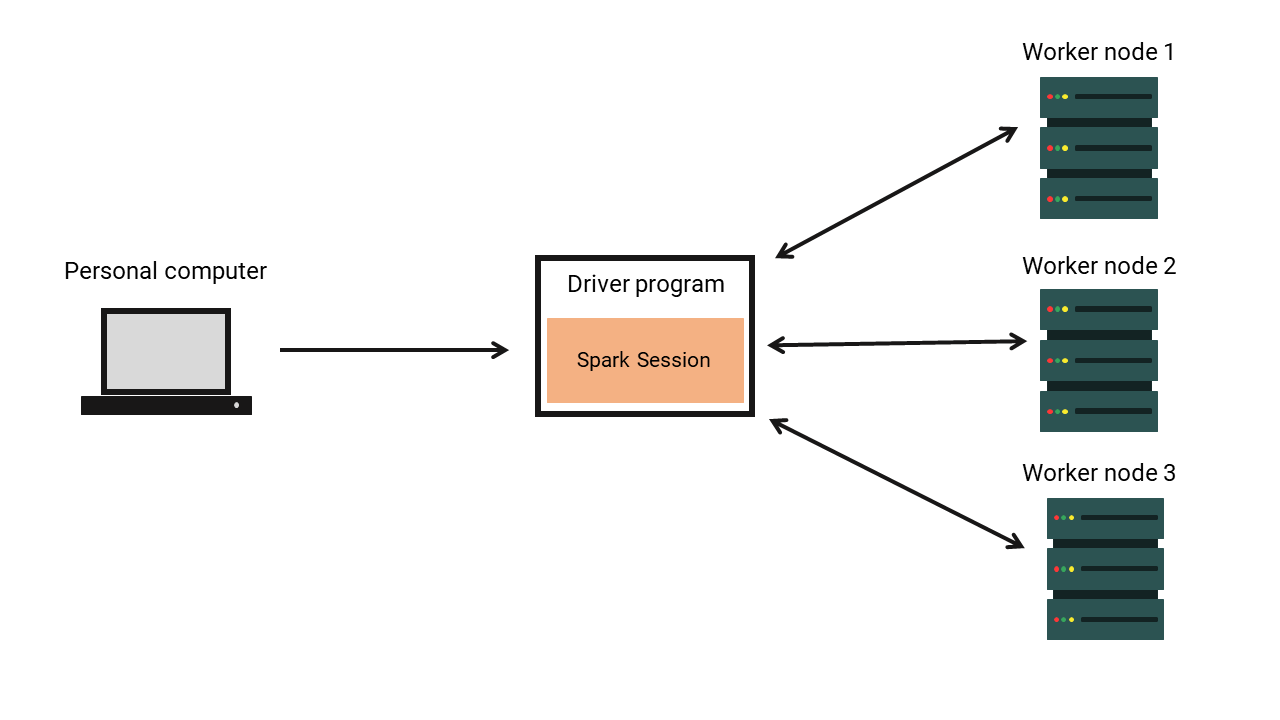
\includegraphics{Chapters/../Figures/spark-application.png}

}

\caption{\label{fig-spark-application}Spark application structure on a
cluster of computers}

\end{figure}

When you run Spark on a cluster of computers, you write the code of your
Spark application (i.e.~your \texttt{pyspark} code) on your (single)
local computer, and then, submit this code to the driver node. After
that, the driver node takes care of the rest, by starting your
application, creating your Spark Session, asking for new worker nodes,
sending the tasks to be performed, collecting and compiling the results
and giving back these results to you.

However, when you run Spark on your (single) local computer, the process
is very similar. But, instead of submitting your code to another
computer (which is the driver node), you will submit to your own local
computer. In other words, when Spark is running on single-node mode,
your computer becomes the driver and the worker node at the same time.

\hypertarget{spark-application-versus-pyspark-application}{%
\section{\texorpdfstring{Spark application versus \texttt{pyspark}
application}{Spark application versus pyspark application}}\label{spark-application-versus-pyspark-application}}

The \texttt{pyspark} package is just a tool to write Spark applications
using the python programming language. This means, that every
\texttt{pyspark} application is a Spark application written in python.

With this conception in mind, you can understand that a \texttt{pyspark}
application is a description of a Spark application. When we compile (or
execute) our python program, this description is translated into a raw
Spark application that will be executed by Spark.

To write a \texttt{pyspark} application, you write a python script that
uses the \texttt{pyspark} library. When you execute this python script
with the python interpreter, the application will be automatically
converted to Spark code, and will be sent to Spark to be executed across
the cluster;

\hypertarget{core-parts-of-a-pyspark-program}{%
\section{\texorpdfstring{Core parts of a \texttt{pyspark}
program}{Core parts of a pyspark program}}\label{core-parts-of-a-pyspark-program}}

In this section, I want to point out the core parts that composes every
\texttt{pyspark} program. This means that every \texttt{pyspark} program
that you write will have these ``core parts'', which are:

\begin{enumerate}
\def\labelenumi{\arabic{enumi})}
\item
  importing the Spark libraries (or packages);
\item
  starting your Spark Session;
\item
  defining a set of transformations and actions over Spark DataFrames;
\end{enumerate}

\hypertarget{importing-the-spark-libraries-or-packages}{%
\subsection{Importing the Spark libraries (or
packages)}\label{importing-the-spark-libraries-or-packages}}

Spark comes with a lot of functionality installed. But, in order to use
it in your \texttt{pyspark} program, you have to import most of these
functionalities to your session. This means that you have to import
specific packages (or ``modules'') of \texttt{pyspark} to your python
session.

For example, most of the functions used to define our transformations
and aggregations in Spark DataFrames, comes from the
\texttt{pyspark.sql.functions} module.

That is why we usually start our python scripts by importing functions
from this module, like this:

\begin{Shaded}
\begin{Highlighting}[]
\ImportTok{from}\NormalTok{ pyspark.sql.functions }\ImportTok{import} \BuiltInTok{sum}\NormalTok{, col}
\NormalTok{sum\_expr }\OperatorTok{=} \BuiltInTok{sum}\NormalTok{(col(}\StringTok{\textquotesingle{}Value\textquotesingle{}}\NormalTok{))}
\end{Highlighting}
\end{Shaded}

Or, importing the entire module with the \texttt{import} keyword, like
this:

\begin{Shaded}
\begin{Highlighting}[]
\ImportTok{import}\NormalTok{ pyspark.sql.functions }\ImportTok{as}\NormalTok{ F}
\NormalTok{sum\_expr }\OperatorTok{=}\NormalTok{ F.}\BuiltInTok{sum}\NormalTok{(F.col(}\StringTok{\textquotesingle{}Value\textquotesingle{}}\NormalTok{))}
\end{Highlighting}
\end{Shaded}

\hypertarget{starting-your-spark-session}{%
\subsection{Starting your Spark
Session}\label{starting-your-spark-session}}

Every Spark application starts with a Spark Session. Basically, the
Spark Session is the entry point to your application. This means that,
in every \texttt{pyspark} program that you write, \textbf{you should
always start by defining your Spark Session}. We do this, by using the
\texttt{getOrCreate()} method from
\texttt{pyspark.sql.SparkSession.builder} module.

Just store the result of this method in any python object. Is very
common to name this object as \texttt{spark}, like in the example below.
This way, you can access all the information and methods of Spark from
this \texttt{spark} object.

\begin{Shaded}
\begin{Highlighting}[]
\ImportTok{from}\NormalTok{ pyspark.sql }\ImportTok{import}\NormalTok{ SparkSession}
\NormalTok{spark }\OperatorTok{=}\NormalTok{ SparkSession.builder.getOrCreate()}
\end{Highlighting}
\end{Shaded}

\hypertarget{defining-a-set-of-transformations-and-actions}{%
\subsection{Defining a set of transformations and
actions}\label{defining-a-set-of-transformations-and-actions}}

Every \texttt{pyspark} program is composed by a set of transformations
and actions over a set of Spark DataFrames.

We will explain Spark DataFrames in more deth on the
Chapter~\ref{sec-dataframes-chapter}. For now just understand that they
are the basic data sctructure that feed all \texttt{pyspark} programs.
In other words, on every \texttt{pyspark} program we are transforming
multiple Spark DataFrames to get the result we want.

As an example, in the script below we begin with the Spark DataFrame
stored in the object \texttt{students}, and, apply multiple
transformations over it to build the \texttt{ar\_department} DataFrame.
Lastly, we apply the \texttt{.show()} action over the
\texttt{ar\_department} DataFrame:

\begin{Shaded}
\begin{Highlighting}[]
\ImportTok{from}\NormalTok{ pyspark.sql.functions }\ImportTok{import}\NormalTok{ col}
\CommentTok{\# Apply some transformations over}
\CommentTok{\# the \textasciigrave{}students\textasciigrave{} DataFrame:}
\NormalTok{ar\_department }\OperatorTok{=}\NormalTok{ students}\OperatorTok{\textbackslash{}}
\NormalTok{  .}\BuiltInTok{filter}\NormalTok{(col(}\StringTok{\textquotesingle{}Age\textquotesingle{}}\NormalTok{) }\OperatorTok{\textgreater{}} \DecValTok{22}\NormalTok{)}\OperatorTok{\textbackslash{}}
\NormalTok{  .withColumn(}\StringTok{\textquotesingle{}IsArDepartment\textquotesingle{}}\NormalTok{, col(}\StringTok{\textquotesingle{}Department\textquotesingle{}}\NormalTok{) }\OperatorTok{==} \StringTok{\textquotesingle{}AR\textquotesingle{}}\NormalTok{)}\OperatorTok{\textbackslash{}}
\NormalTok{  .orderBy(col(}\StringTok{\textquotesingle{}Age\textquotesingle{}}\NormalTok{).desc())}
  
  
\CommentTok{\# Apply the \textasciigrave{}.show()\textasciigrave{} action}
\CommentTok{\# over the \textasciigrave{}ar\_department\textasciigrave{} DataFrame:}
\NormalTok{ar\_department.show()}
\end{Highlighting}
\end{Shaded}

\hypertarget{building-your-first-spark-application}{%
\section{Building your first Spark
application}\label{building-your-first-spark-application}}

To demonstrate what a \texttt{pyspark} program looks like, lets write
and run our first example of a Spark application. This Spark application
will build a simple table of 1 column that contains 5 numbers, and then,
it will return a simple python list containing this five numbers as a
result.

\hypertarget{writing-the-code}{%
\subsection{Writing the code}\label{writing-the-code}}

First, create a new blank text file in your computer, and save it
somewhere with the name \texttt{spark-example.py}. Do not forget to put
the \texttt{.py} extension in the name. This program we are writing
together is a python program, and should be treated as such. With the
\texttt{.py} extension in the name file, you are stating this fact quite
clearly to your computer.

After you created and saved the python script (i.e.~the text file with
the \texttt{.py} extension), you can start writing your \texttt{pyspark}
program. As we noted in the previous section, you should always start
your \texttt{pyspark} program by defining your Spark Session, with this
code:

\begin{Shaded}
\begin{Highlighting}[]
\ImportTok{from}\NormalTok{ pyspark.sql }\ImportTok{import}\NormalTok{ SparkSession}
\NormalTok{spark }\OperatorTok{=}\NormalTok{ SparkSession.builder.getOrCreate()}
\end{Highlighting}
\end{Shaded}

After you defined your Spark Session, and saved it in an object called
\texttt{spark}, you can now access all Spark's functionality through
this \texttt{spark} object.

To create our first Spark table we use the \texttt{range()} method from
the \texttt{spark} object. The \texttt{range()} method works similarly
as the standard python function called \texttt{range()}. It basically
creates a sequence of numbers, from 0 to \(n - 1\). However, this
\texttt{range()} method from \texttt{spark} stores this sequence of
numbers as rows in a Spark table (or a Spark DataFrame):

\begin{Shaded}
\begin{Highlighting}[]
\NormalTok{table }\OperatorTok{=}\NormalTok{ spark.}\BuiltInTok{range}\NormalTok{(}\DecValTok{5}\NormalTok{)}
\end{Highlighting}
\end{Shaded}

After this step, we want to collect all the rows of the resulting table
into a python list. And to do that, we use the \texttt{collect()} method
from the Spark table:

\begin{Shaded}
\begin{Highlighting}[]
\NormalTok{result }\OperatorTok{=}\NormalTok{ table.collect()}
\BuiltInTok{print}\NormalTok{(result)}
\end{Highlighting}
\end{Shaded}

So, the entire program is composed of these three parts (or sections) of
code. If you need it, the entire program is reproduced below. You can
copy and paste all of this code to your python script, and then, save
it:

\begin{Shaded}
\begin{Highlighting}[]
\CommentTok{\# The entire program:}
\ImportTok{from}\NormalTok{ pyspark.sql }\ImportTok{import}\NormalTok{ SparkSession}
\NormalTok{spark }\OperatorTok{=}\NormalTok{ SparkSession.builder.getOrCreate()}

\NormalTok{table }\OperatorTok{=}\NormalTok{ spark.}\BuiltInTok{range}\NormalTok{(}\DecValTok{5}\NormalTok{)}
\NormalTok{result }\OperatorTok{=}\NormalTok{ table.collect()}
\BuiltInTok{print}\NormalTok{(result)}
\end{Highlighting}
\end{Shaded}

\hypertarget{executing-the-code}{%
\subsection{Executing the code}\label{executing-the-code}}

Now that you have written your first Spark application with
\texttt{pyspark}, you want to execute this application and see its
results. Yet, to run a \texttt{pyspark} program, remember that you need
to have the necessary software installed on your machine. I talk about
how to install these software at Appendix~\ref{sec-install-spark}.

Anyway, to execute this \texttt{pyspark} that you wrote, you need send
this script to the python interpreter, and to do this you need to: 1)
open a terminal inside the folder where you python script is stored;
and, 2) use the python command from the terminal with the name of your
python script.

If you do not know how to open a terminal from inside a folder of your
computer, you can consult Appendix~\ref{sec-open-terminal} of this book,
where I teach you how to do it.

In my current situation, I running Spark on a Ubuntu distribution, and,
I saved the \texttt{spark-example.py} script inside a folder called
\texttt{SparkExample}. This folder is located at the path
\texttt{\textasciitilde{}/Documentos/Projetos/Livros/Introd-pyspark/SparkExample}
of my computer. This means that, I need to open a terminal that is
rooted inside this \texttt{SparkExample} folder.

You probably have saved your \texttt{spark-example.py} file in a
different folder of your computer. This means that you need to open the
terminal from a different folder.

After I opened a terminal rooted inside the \texttt{SparkExample}
folder. I just use the \texttt{python3} command to access the python
interpreter, and, give the name of the python script that I want to
execute. In this case, the \texttt{spark-example.py} file. As a result,
our first \texttt{pyspark} program will be executed:

\begin{Shaded}
\begin{Highlighting}[]
\NormalTok{Terminal$ python3 spark{-}example.py}
\end{Highlighting}
\end{Shaded}

\begin{verbatim}
[Row(id=0), Row(id=1), Row(id=2), Row(id=3), Row(id=4)]
\end{verbatim}

You can see in the above result, that this Spark application produces a
sequence of numbers, from 0 to 4, and, returns this sequence as a set of
\texttt{Row} objects, inside a python list.

Congratulations! You have just run your first Spark application using
\texttt{pyspark}!

\hypertarget{overview-of-pyspark}{%
\section{\texorpdfstring{Overview of
\texttt{pyspark}}{Overview of pyspark}}\label{overview-of-pyspark}}

Before we continue, I want to give you a very brief overview of the main
parts of \texttt{pyspark} that are the most useful and most important to
know of.

\hypertarget{main-python-modules}{%
\subsection{Main python modules}\label{main-python-modules}}

The main python modules that exists in \texttt{pyspark} are:

\begin{itemize}
\tightlist
\item
  \texttt{pyspark.sql.SparkSession}: the \texttt{SparkSession} class
  that defines your Spark Session, or, the entry point to your Spark
  application;
\item
  \texttt{pyspark.sql.dataframe}: module that defines the
  \texttt{DataFrame} class;
\item
  \texttt{pyspark.sql.column}: module that defines the \texttt{Column}
  class;
\item
  \texttt{pyspark.sql.types}: module that contains all data types of
  Spark;
\item
  \texttt{pyspark.sq.functions}: module that contains all of the main
  Spark functions that we use in transformations;
\item
  \texttt{pyspark.sql.window}: module that defines the \texttt{Window}
  class, which is responsible for defining windows in a Spark DataFrame;
\end{itemize}

\hypertarget{main-python-classes}{%
\subsection{Main python classes}\label{main-python-classes}}

The main python classes that exists in \texttt{pyspark} are:

\begin{itemize}
\item
  \texttt{DataFrame}: represents a Spark DataFrame, and it is the main
  data structure in \texttt{pyspark}. In essence, they represent a
  collection of datasets into named columns;
\item
  \texttt{Column}: represents a column in a Spark DataFrame;
\item
  \texttt{GroupedData}: represents a grouped Spark DataFrame (result of
  \texttt{DataFrame.groupby()});
\item
  \texttt{Window}: describes a window in a Spark DataFrame;
\item
  \texttt{DataFrameReader} and \texttt{DataFrameWriter}: classes
  responsible for reading data from a data source into a Spark
  DataFrame, and writing data from a Spark DataFrame into a data source;
\item
  \texttt{DataFrameNaFunctions}: class that stores all main methods for
  dealing with null values (i.e.~missing data);
\end{itemize}

\bookmarksetup{startatroot}

\hypertarget{sec-dataframes-chapter}{%
\chapter{Introducing Spark DataFrames}\label{sec-dataframes-chapter}}

\hypertarget{introduction-3}{%
\section{Introduction}\label{introduction-3}}

In this chapter, you will understand how Spark represents and manages
tables (or tabular data). Different programming languages and frameworks
use different names to describe a table. But, in Apache Spark, they are
referred as Spark DataFrames.

In \texttt{pyspark}, these DataFrames are stored inside python objects
of class \texttt{pyspark.sql.dataframe.DataFrame}, and all the methods
present in this class, are commonly referred as the DataFrame API of
Spark. This is the most important API of Spark, because much of your
Spark applications will heavily use this API to compose your data
transformations and data flows (Chambers and Zaharia 2018).

\hypertarget{spark-dataframes-versus-spark-datasets}{%
\section{Spark DataFrames versus Spark
Datasets}\label{spark-dataframes-versus-spark-datasets}}

Spark have two notions of structured data: DataFrames and Datasets. In
summary, a Spark Dataset, is a distributed collection of data
(\emph{Apache Spark Official Documentation} 2022). In contrast, a Spark
DataFrame is a Spark Dataset organized into named columns (\emph{Apache
Spark Official Documentation} 2022).

This means that, Spark DataFrames are very similar to tables as we know
in relational databases - RDBMS, or, in spreadsheets (like Excel). So in
a Spark DataFrame, each column has a name, and they all have the same
number of rows. Furthermore, all the rows inside a column must store the
same type of data, but each column can store a different type of data.

In the other hand, Spark Datasets are considered a collection of any
type of data. So a Dataset might be a collection of unstructured data as
well, like log files, JSON and XML trees, etc. Spark Datasets can be
created and transformed trough the Dataset API of Spark. But this API is
available only in Scala and Java API's of Spark. For this reason, we do
not act directly on Datasets with \texttt{pyspark}, only DataFrames.
That's ok, because for the most part of applications, we do want to use
DataFrames, and not Datasets, to represent our data.

However, what makes a Spark DataFrame different from other dataframes?
Like the \texttt{pandas} DataFrame? Or the R native \texttt{data.frame}
structure? Is the \textbf{distributed} aspect of it. Spark DataFrames
are based on Spark Datasets, and these Datasets are collections of data
that are distributed across the cluster. As an example, lets suppose you
have the following table stored as a Spark DataFrame:

\begin{longtable}[]{@{}lll@{}}
\toprule()
ID & Name & Value \\
\midrule()
\endhead
1 & Anne & 502 \\
2 & Carls & 432 \\
3 & Stoll & 444 \\
4 & Percy & 963 \\
5 & Martha & 123 \\
6 & Sigrid & 621 \\
\bottomrule()
\end{longtable}

If you are running Spark in a 4 nodes cluster (one is the driver node,
and the other three are worker nodes). Each worker node of the cluster
will store a section of this data. So you, as the programmer, will see,
manage and transform this table as if it was a single and unified table.
But behind the hoods, Spark will split this data and store it as many
fragments across the Spark cluster. Figure~\ref{fig-distributed-df}
presents this notion in a visual manner.

\begin{figure}

{\centering 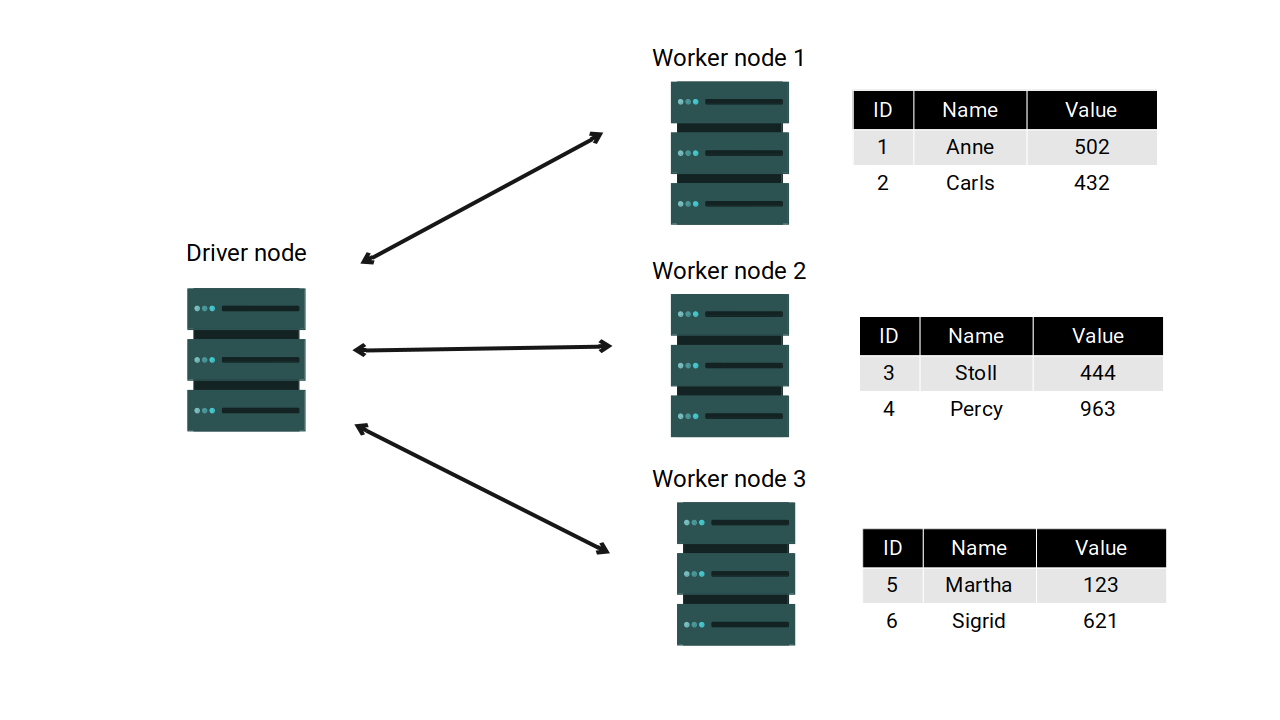
\includegraphics{Chapters/../Figures/distributed-df.png}

}

\caption{\label{fig-distributed-df}A Spark DataFrame is distributed
across the cluster}

\end{figure}

\hypertarget{partitions-of-a-spark-dataframe}{%
\section{Partitions of a Spark
DataFrame}\label{partitions-of-a-spark-dataframe}}

A Spark DataFrame is always broken into many small pieces, and, these
pieces are always spread across the cluster of machines. Each one of
these small pieces of the total data are considered a DataFrame
\emph{partition}.

For the most part, you do not manipulate these partitions manually or
individually (Karau et al. 2015), because Spark automatically do this
job for you.

As we exposed in Figure~\ref{fig-distributed-df}, each node of the
cluster will hold a piece of the total DataFrame. If we translate this
distribution into a ``partition'' distribution, this means that each
node of the cluster can hold one or multiple partitions of the Spark
DataFrame.

If we sum all partitions present in a node of the cluster, we get a
chunk of the total DataFrame. The figure below demonstrates this notion:

\begin{figure}

{\centering 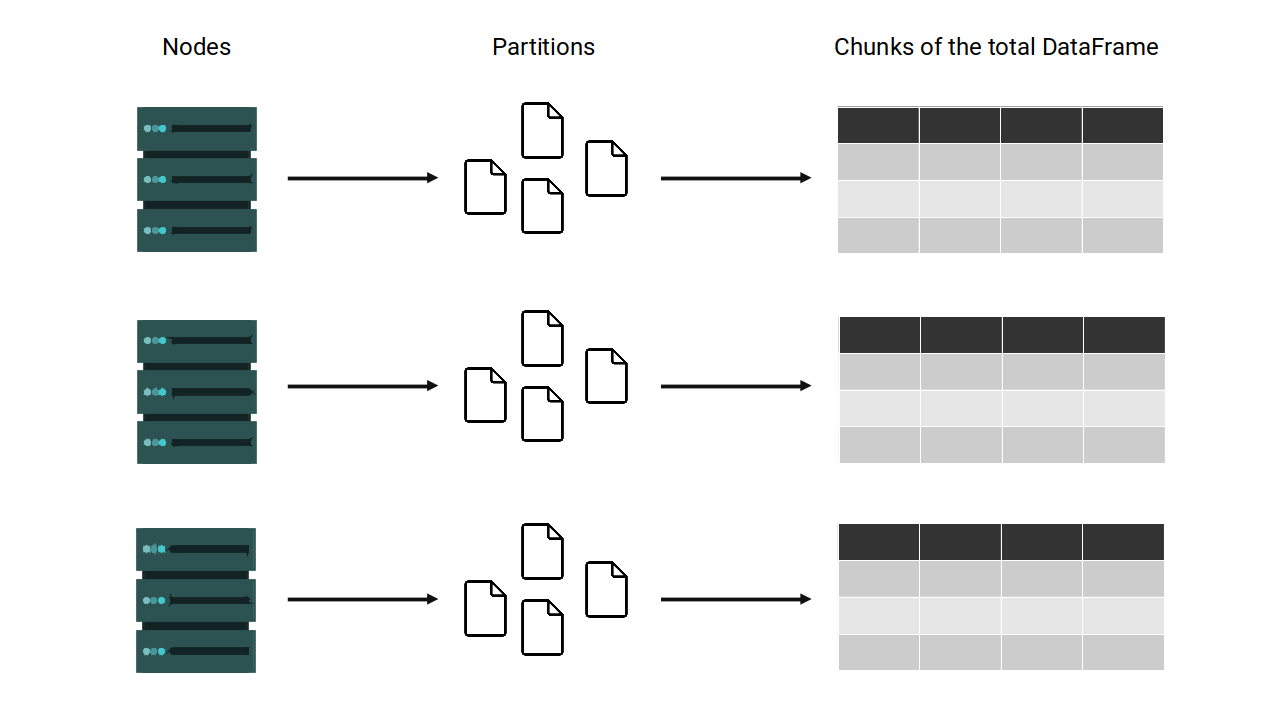
\includegraphics{Chapters/../Figures/partitions-df.png}

}

\caption{\label{fig-partitions-df}Partitions of a DataFrame}

\end{figure}

If the Spark DataFrame is not big, each node of the cluster will
probably store just a single partition of this DataFrame. In contrast,
depending on the complexity and size of the DataFrame, Spark will split
this DataFrame into more partitions that there are nodes in the cluster.
In this case, each node of the cluster will hold more than 1 partition
of the total DataFrame.

\hypertarget{sec-dataframe-class}{%
\section{\texorpdfstring{The \texttt{DataFrame} class in
\texttt{pyspark}}{The DataFrame class in pyspark}}\label{sec-dataframe-class}}

In \texttt{pyspark}, every Spark DataFrame is stored inside a python
object of class \texttt{pyspark.sql.dataframe.DataFrame}. Or more
succintly, a object of class \texttt{DataFrame}.

Like any python class, the \texttt{DataFrame} class comes with multiple
methods that are available for every object of this class. This means
that you can use any of these methods in any Spark DataFrame that you
create through \texttt{pyspark}.

As an example, in the code below I expose all the available methods from
this \texttt{DataFrame} class. First, I create a Spark DataFrame with
\texttt{spark.range(5)}, and, store it in the object \texttt{df5}. After
that, I use the \texttt{dir()} function to show all the methods that I
can use through this \texttt{df5} object:

\begin{Shaded}
\begin{Highlighting}[]
\NormalTok{df5 }\OperatorTok{=}\NormalTok{ spark.}\BuiltInTok{range}\NormalTok{(}\DecValTok{5}\NormalTok{)}
\NormalTok{available\_methods }\OperatorTok{=} \BuiltInTok{dir}\NormalTok{(df5)}
\BuiltInTok{print}\NormalTok{(available\_methods)}
\end{Highlighting}
\end{Shaded}

\begin{verbatim}
['__class__', '__delattr__', '__dict__', '__dir__',
'__doc__', '__eq__', '__format__', '__ge__',
'__getattr__', '__getattribute__', '__getitem__', '__gt__',
'__hash__', '__init__', '__init_subclass__', '__le__',
'__lt__', '__module__', '__ne__', '__new__',
'__reduce__', '__reduce_ex__', '__repr__', '__setattr__',
'__sizeof__', '__str__', '__subclasshook__', '__weakref__',
'_collect_as_arrow', '_jcols', '_jdf', '_jmap',
'_joinAsOf', '_jseq', '_lazy_rdd', '_repr_html_',
'_sc', '_schema', '_session', '_sort_cols',
'_sql_ctx', '_support_repr_html', '_to_corrected_pandas_type', 'agg',
'alias', 'approxQuantile', 'cache', 'checkpoint',
'coalesce', 'colRegex', 'collect', 'columns',
'corr', 'count', 'cov', 'createGlobalTempView',
'createOrReplaceGlobalTempView', 'createOrReplaceTempView', 'createTempView', 'crossJoin',
'crosstab', 'cube', 'describe', 'distinct',
'drop', 'dropDuplicates', 'drop_duplicates', 'dropna',
'dtypes', 'exceptAll', 'explain', 'fillna',
'filter', 'first', 'foreach', 'foreachPartition',
'freqItems', 'groupBy', 'groupby', 'head',
'hint', 'inputFiles', 'intersect', 'intersectAll',
'isEmpty', 'isLocal', 'isStreaming', 'is_cached',
'join', 'limit', 'localCheckpoint', 'mapInArrow',
'mapInPandas', 'na', 'observe', 'orderBy',
'pandas_api', 'persist', 'printSchema', 'randomSplit',
'rdd', 'registerTempTable', 'repartition', 'repartitionByRange',
'replace', 'rollup', 'sameSemantics', 'sample',
'sampleBy', 'schema', 'select', 'selectExpr',
'semanticHash', 'show', 'sort', 'sortWithinPartitions',
'sparkSession', 'sql_ctx', 'stat', 'storageLevel',
'subtract', 'summary', 'tail', 'take',
'toDF', 'toJSON', 'toLocalIterator', 'toPandas',
'to_koalas', 'to_pandas_on_spark', 'transform', 'union',
'unionAll', 'unionByName', 'unpersist', 'where',
'withColumn', 'withColumnRenamed', 'withColumns', 'withMetadata',
'withWatermark', 'write', 'writeStream', 'writeTo'],
\end{verbatim}

All the methods present in this \texttt{DataFrame} class, are commonly
referred as the \emph{DataFrame API of Spark}. Remember, this is the
most important API of Spark. Because much of your Spark applications
will heavily use this API to compose your data transformations and data
flows (Chambers and Zaharia 2018).

\hypertarget{sec-building-a-dataframe}{%
\section{Building a Spark DataFrame}\label{sec-building-a-dataframe}}

There are some different methods to create a Spark DataFrame. For
example, because a DataFrame is basically a Dataset of rows, we can
build a DataFrame from a collection of \texttt{Row}'s, through the
\texttt{createDataFrame()} method from your Spark Session:

\begin{Shaded}
\begin{Highlighting}[]
\ImportTok{from}\NormalTok{ pyspark.sql }\ImportTok{import}\NormalTok{ SparkSession}
\NormalTok{spark }\OperatorTok{=}\NormalTok{ SparkSession.builder.getOrCreate()}
\ImportTok{from}\NormalTok{ datetime }\ImportTok{import}\NormalTok{ date}
\ImportTok{from}\NormalTok{ pyspark.sql }\ImportTok{import}\NormalTok{ Row}

\NormalTok{data }\OperatorTok{=}\NormalTok{ [}
\NormalTok{  Row(}\BuiltInTok{id} \OperatorTok{=} \DecValTok{1}\NormalTok{, value }\OperatorTok{=} \FloatTok{28.3}\NormalTok{, date }\OperatorTok{=}\NormalTok{ date(}\DecValTok{2021}\NormalTok{,}\DecValTok{1}\NormalTok{,}\DecValTok{1}\NormalTok{)),}
\NormalTok{  Row(}\BuiltInTok{id} \OperatorTok{=} \DecValTok{2}\NormalTok{, value }\OperatorTok{=} \FloatTok{15.8}\NormalTok{, date }\OperatorTok{=}\NormalTok{ date(}\DecValTok{2021}\NormalTok{,}\DecValTok{1}\NormalTok{,}\DecValTok{1}\NormalTok{)),}
\NormalTok{  Row(}\BuiltInTok{id} \OperatorTok{=} \DecValTok{3}\NormalTok{, value }\OperatorTok{=} \FloatTok{20.1}\NormalTok{, date }\OperatorTok{=}\NormalTok{ date(}\DecValTok{2021}\NormalTok{,}\DecValTok{1}\NormalTok{,}\DecValTok{2}\NormalTok{)),}
\NormalTok{  Row(}\BuiltInTok{id} \OperatorTok{=} \DecValTok{4}\NormalTok{, value }\OperatorTok{=} \FloatTok{12.6}\NormalTok{, date }\OperatorTok{=}\NormalTok{ date(}\DecValTok{2021}\NormalTok{,}\DecValTok{1}\NormalTok{,}\DecValTok{3}\NormalTok{))}
\NormalTok{]}

\NormalTok{df }\OperatorTok{=}\NormalTok{ spark.createDataFrame(data)}
\end{Highlighting}
\end{Shaded}

Remember that a Spark DataFrame in python is a object of class
\texttt{pyspark.sql.dataframe.DataFrame} as you can see below:

\begin{Shaded}
\begin{Highlighting}[]
\BuiltInTok{type}\NormalTok{(df)}
\end{Highlighting}
\end{Shaded}

\begin{verbatim}
pyspark.sql.dataframe.DataFrame
\end{verbatim}

If you try to see what is inside of this kind of object, you will get a
small description of the columns present in the DataFrame as a result:

\begin{Shaded}
\begin{Highlighting}[]
\NormalTok{df}
\end{Highlighting}
\end{Shaded}

\begin{verbatim}
DataFrame[id: bigint, value: double, date: date]
\end{verbatim}

So, in the above example, we use the \texttt{Row()} constructor (from
\texttt{pyspark.sql} module) to build 4 rows. The
\texttt{createDataFrame()} method, stack these 4 rows together to form
our new DataFrame \texttt{df}. The result is a Spark DataFrame with 4
rows and 3 columns (\texttt{id}, \texttt{value} and \texttt{date}).

But you can use different methods to create the same Spark DataFrame. As
another example, with the code below, we are creating a DataFrame called
\texttt{students} from two different python lists (\texttt{data} and
\texttt{columns}).

The first list (\texttt{data}) is a list of rows. Each row is represent
by a python tuple, which contains the values in each column. But the
secont list (\texttt{columns}) contains the names for each column in the
DataFrame.

To create the \texttt{students} DataFrame we deliver these two lists to
\texttt{createDataFrame()} method:

\begin{Shaded}
\begin{Highlighting}[]
\NormalTok{data }\OperatorTok{=}\NormalTok{ [}
\NormalTok{  (}\DecValTok{12114}\NormalTok{, }\StringTok{\textquotesingle{}Anne\textquotesingle{}}\NormalTok{, }\DecValTok{21}\NormalTok{, }\FloatTok{1.56}\NormalTok{, }\DecValTok{8}\NormalTok{, }\DecValTok{9}\NormalTok{, }\DecValTok{10}\NormalTok{, }\DecValTok{9}\NormalTok{, }\StringTok{\textquotesingle{}Economics\textquotesingle{}}\NormalTok{, }\StringTok{\textquotesingle{}SC\textquotesingle{}}\NormalTok{),}
\NormalTok{  (}\DecValTok{13007}\NormalTok{, }\StringTok{\textquotesingle{}Adrian\textquotesingle{}}\NormalTok{, }\DecValTok{23}\NormalTok{, }\FloatTok{1.82}\NormalTok{, }\DecValTok{6}\NormalTok{, }\DecValTok{6}\NormalTok{, }\DecValTok{8}\NormalTok{, }\DecValTok{7}\NormalTok{, }\StringTok{\textquotesingle{}Economics\textquotesingle{}}\NormalTok{, }\StringTok{\textquotesingle{}SC\textquotesingle{}}\NormalTok{),}
\NormalTok{  (}\DecValTok{10045}\NormalTok{, }\StringTok{\textquotesingle{}George\textquotesingle{}}\NormalTok{, }\DecValTok{29}\NormalTok{, }\FloatTok{1.77}\NormalTok{, }\DecValTok{10}\NormalTok{, }\DecValTok{9}\NormalTok{, }\DecValTok{10}\NormalTok{, }\DecValTok{7}\NormalTok{, }\StringTok{\textquotesingle{}Law\textquotesingle{}}\NormalTok{, }\StringTok{\textquotesingle{}SC\textquotesingle{}}\NormalTok{),}
\NormalTok{  (}\DecValTok{12459}\NormalTok{, }\StringTok{\textquotesingle{}Adeline\textquotesingle{}}\NormalTok{, }\DecValTok{26}\NormalTok{, }\FloatTok{1.61}\NormalTok{, }\DecValTok{8}\NormalTok{, }\DecValTok{6}\NormalTok{, }\DecValTok{7}\NormalTok{, }\DecValTok{7}\NormalTok{, }\StringTok{\textquotesingle{}Law\textquotesingle{}}\NormalTok{, }\StringTok{\textquotesingle{}SC\textquotesingle{}}\NormalTok{),}
\NormalTok{  (}\DecValTok{10190}\NormalTok{, }\StringTok{\textquotesingle{}Mayla\textquotesingle{}}\NormalTok{, }\DecValTok{22}\NormalTok{, }\FloatTok{1.67}\NormalTok{, }\DecValTok{7}\NormalTok{, }\DecValTok{7}\NormalTok{, }\DecValTok{7}\NormalTok{, }\DecValTok{9}\NormalTok{, }\StringTok{\textquotesingle{}Design\textquotesingle{}}\NormalTok{, }\StringTok{\textquotesingle{}AR\textquotesingle{}}\NormalTok{),}
\NormalTok{  (}\DecValTok{11552}\NormalTok{, }\StringTok{\textquotesingle{}Daniel\textquotesingle{}}\NormalTok{, }\DecValTok{24}\NormalTok{, }\FloatTok{1.75}\NormalTok{, }\DecValTok{9}\NormalTok{, }\DecValTok{9}\NormalTok{, }\DecValTok{10}\NormalTok{, }\DecValTok{9}\NormalTok{, }\StringTok{\textquotesingle{}Design\textquotesingle{}}\NormalTok{, }\StringTok{\textquotesingle{}AR\textquotesingle{}}\NormalTok{)}
\NormalTok{]}

\NormalTok{columns }\OperatorTok{=}\NormalTok{ [}
  \StringTok{\textquotesingle{}StudentID\textquotesingle{}}\NormalTok{, }\StringTok{\textquotesingle{}Name\textquotesingle{}}\NormalTok{, }\StringTok{\textquotesingle{}Age\textquotesingle{}}\NormalTok{, }\StringTok{\textquotesingle{}Height\textquotesingle{}}\NormalTok{, }\StringTok{\textquotesingle{}Score1\textquotesingle{}}\NormalTok{,}
  \StringTok{\textquotesingle{}Score2\textquotesingle{}}\NormalTok{, }\StringTok{\textquotesingle{}Score3\textquotesingle{}}\NormalTok{, }\StringTok{\textquotesingle{}Score4\textquotesingle{}}\NormalTok{, }\StringTok{\textquotesingle{}Course\textquotesingle{}}\NormalTok{, }\StringTok{\textquotesingle{}Department\textquotesingle{}}
\NormalTok{]}

\NormalTok{students }\OperatorTok{=}\NormalTok{ spark.createDataFrame(data, columns)}
\NormalTok{students}
\end{Highlighting}
\end{Shaded}

\begin{verbatim}
DataFrame[StudentID: bigint, Name: string, Age: bigint, Height: double, Score1: bigint, Score2: bigint, Score3: bigint, Score4: bigint, Course: string, Department: string]
\end{verbatim}

You can also use a method that returns a \texttt{DataFrame} object by
default. Examples are the \texttt{table()} and \texttt{range()} methods
from your Spark Session, like we used in the
Section~\ref{sec-dataframe-class}, to create the \texttt{df5} object.

Other examples are the methods used to read data and import it to
\texttt{pyspark}. These methods are available in the \texttt{spark.read}
module, like \texttt{spark.read.csv()} and \texttt{spark.read.json()}.
These methods will be described in more depth in
Chapter~\ref{sec-import-export}.

\hypertarget{sec-viewing-a-dataframe}{%
\section{Viewing a Spark DataFrame}\label{sec-viewing-a-dataframe}}

A key aspect of Spark is its laziness. In other words, for most
operations, Spark will only check if your code is correct and if it
makes sense. Spark will not actually run or execute the operations you
are describing in your code, unless you explicit ask for it with a
trigger operation, which is called an ``action'' (this kind of operation
is described in Section~\ref{sec-dataframe-actions}).

You can notice this laziness in the output below:

\begin{Shaded}
\begin{Highlighting}[]
\NormalTok{students}
\end{Highlighting}
\end{Shaded}

\begin{verbatim}
DataFrame[StudentID: bigint, Name: string, Age: bigint, Height: double, Score1: bigint, Score2: bigint, Score3: bigint, Score4: bigint, Course: string, Department: string]
\end{verbatim}

Because when we call for an object that stores a Spark DataFrame (like
\texttt{df} and \texttt{students}), Spark will only calculate and print
a summary of the structure of your Spark DataFrame, and not the
DataFrame itself.

So how can we actually see our DataFrame? How can we visualize the rows
and values that are stored inside of it? For this, we use the
\texttt{show()} method. With this method, Spark will print the table as
pure text, as you can see in the example below:

\begin{Shaded}
\begin{Highlighting}[]
\NormalTok{students.show()}
\end{Highlighting}
\end{Shaded}

\begin{verbatim}
[Stage 0:>                                                          (0 + 1) / 1]                                                                                
\end{verbatim}

\begin{verbatim}
+---------+-------+---+------+------+------+------+------+---------+----------+
|StudentID|   Name|Age|Height|Score1|Score2|Score3|Score4|   Course|Department|
+---------+-------+---+------+------+------+------+------+---------+----------+
|    12114|   Anne| 21|  1.56|     8|     9|    10|     9|Economics|        SC|
|    13007| Adrian| 23|  1.82|     6|     6|     8|     7|Economics|        SC|
|    10045| George| 29|  1.77|    10|     9|    10|     7|      Law|        SC|
|    12459|Adeline| 26|  1.61|     8|     6|     7|     7|      Law|        SC|
|    10190|  Mayla| 22|  1.67|     7|     7|     7|     9|   Design|        AR|
|    11552| Daniel| 24|  1.75|     9|     9|    10|     9|   Design|        AR|
+---------+-------+---+------+------+------+------+------+---------+----------+
\end{verbatim}

By default, this method shows only the top rows of your DataFrame, but
you can specify how much rows exactly you want to see, by using
\texttt{show(n)}, where \texttt{n} is the number of rows. For example, I
can visualize only the first 2 rows of \texttt{df} like this:

\begin{Shaded}
\begin{Highlighting}[]
\NormalTok{df.show(}\DecValTok{2}\NormalTok{)}
\end{Highlighting}
\end{Shaded}

\begin{verbatim}
+---+-----+----------+
| id|value|      date|
+---+-----+----------+
|  1| 28.3|2021-01-01|
|  2| 15.8|2021-01-01|
+---+-----+----------+
only showing top 2 rows
\end{verbatim}

\hypertarget{getting-the-name-of-the-columns}{%
\section{Getting the name of the
columns}\label{getting-the-name-of-the-columns}}

If you need to, you can easily collect a python list with the column
names present in your DataFrame, in the same way you would do in a
\texttt{pandas} DataFrame. That is, by using the \texttt{columns} method
of your DataFrame, like this:

\begin{Shaded}
\begin{Highlighting}[]
\NormalTok{students.columns}
\end{Highlighting}
\end{Shaded}

\begin{verbatim}
['StudentID',
 'Name',
 'Age',
 'Height',
 'Score1',
 'Score2',
 'Score3',
 'Score4',
 'Course',
 'Department']
\end{verbatim}

\hypertarget{spark-data-types}{%
\section{Spark Data Types}\label{spark-data-types}}

Each column of your Spark DataFrame is associated with a specific data
type. Spark supports a large number of different data types. You can see
the full list at the official documentation page\footnote{The full list
  is available at the link
  \url{https://spark.apache.org/docs/3.3.0/sql-ref-datatypes.html\#supported-data-types}}.
For now, we will focus on the most used data types, which are listed
below:

\begin{itemize}
\tightlist
\item
  \texttt{IntegerType}: Represents 4-byte signed integer numbers. The
  range of numbers that it can represent is from -2147483648 to
  2147483647.
\item
  \texttt{LongType}: Represents 8-byte signed integer numbers. The range
  of numbers that it can represent is from -9223372036854775808 to
  9223372036854775807.
\item
  \texttt{FloatType}: Represents 4-byte single-precision floating point
  numbers.
\item
  \texttt{DoubleType}: Represents 8-byte double-precision floating point
  numbers.
\item
  \texttt{StringType}: Represents character string values.
\item
  \texttt{BooleanType}: Represents boolean values (true or false).
\item
  \texttt{TimestampType}: Represents datetime values, i.e.~values that
  contains fields year, month, day, hour, minute, and second, with the
  session local time-zone. The timestamp value represents an absolute
  point in time.
\item
  \texttt{DateType}: Represents date values, i.e.~values that contains
  fields year, month and day, without a time-zone.
\end{itemize}

Besides these more ``standard'' data types, Spark supports two other
complex types, which are \texttt{ArrayType} and \texttt{MapType}:

\begin{itemize}
\item
  \texttt{ArrayType(elementType,\ containsNull)}: Represents a sequence
  of elements with the type of \texttt{elementType}.
  \texttt{containsNull} is used to indicate if elements in a
  \texttt{ArrayType} value can have \texttt{null} values.
\item
  \texttt{MapType(keyType,\ valueType,\ valueContainsNull)}: Represents
  a set of key-value pairs. The data type of keys is described by
  \texttt{keyType} and the data type of values is described by
  \texttt{valueType}. For a \texttt{MapType} value, keys are not allowed
  to have \texttt{null} values. \texttt{valueContainsNull} is used to
  indicate if values of a \texttt{MapType} value can have \texttt{null}
  values.
\end{itemize}

Each one of these Spark data types have a corresponding python class in
\texttt{pyspark}, which are stored in the \texttt{pyspark.sql.types}
module. As a result, to access, lets say, type \texttt{StryngType}, we
can do this:

\begin{Shaded}
\begin{Highlighting}[]
\ImportTok{from}\NormalTok{ pyspark.sql.types }\ImportTok{import}\NormalTok{ StringType}
\NormalTok{s }\OperatorTok{=}\NormalTok{ StringType()}
\BuiltInTok{print}\NormalTok{(s)}
\end{Highlighting}
\end{Shaded}

\begin{verbatim}
StringType()
\end{verbatim}

\hypertarget{the-dataframe-schema}{%
\section{The DataFrame Schema}\label{the-dataframe-schema}}

The schema of a Spark DataFrame is the combination of column names and
the data types associated with each of these columns. Schemas can be set
explicitly by you (that is, you can tell Spark how the schema of your
DataFrame should look like), or, they can be automatically defined by
Spark while reading or creating your data.

You can get a succinct description of a DataFrame schema, by looking
inside the object where this DataFrame is stored. For example, lets look
again to the \texttt{df} DataFrame.

In the result below, we can see that \texttt{df} has three columns
(\texttt{id}, \texttt{value} and \texttt{date}). By the description
\texttt{id:\ bigint}, we know that \texttt{id} is a column of type
\texttt{bigint}, which translates to the \texttt{LongType()} of Spark.
Furthermore, by the descriptions \texttt{value:\ double} and
\texttt{date:\ date}, we know too that the columns \texttt{value} and
\texttt{date} are of type \texttt{DoubleType()} and \texttt{DateType()},
respectively.

\begin{Shaded}
\begin{Highlighting}[]
\NormalTok{df}
\end{Highlighting}
\end{Shaded}

\begin{verbatim}
DataFrame[id: bigint, value: double, date: date]
\end{verbatim}

You can also visualize a more complete report of the DataFrame schema by
using the \texttt{printSchema()} method, like this:

\begin{Shaded}
\begin{Highlighting}[]
\NormalTok{df.printSchema()}
\end{Highlighting}
\end{Shaded}

\begin{verbatim}
root
 |-- id: long (nullable = true)
 |-- value: double (nullable = true)
 |-- date: date (nullable = true)
\end{verbatim}

\hypertarget{accessing-the-dataframe-schema}{%
\subsection{Accessing the DataFrame
schema}\label{accessing-the-dataframe-schema}}

So, by calling the object of your DataFrame (i.e.~an object of class
\texttt{DataFrame}) you can see a small description of the schema of
this DataFrame. But, how can you access this schema programmatically?

You do this, by using the \texttt{schema} method of your DataFrame, like
in the example below:

\begin{Shaded}
\begin{Highlighting}[]
\NormalTok{df.schema}
\end{Highlighting}
\end{Shaded}

\begin{verbatim}
StructType([StructField('id', LongType(), True), StructField('value', DoubleType(), True), StructField('date', DateType(), True)])
\end{verbatim}

The result of the \texttt{schema} method, is a \texttt{StructType()}
object, that contains some information about each column of your
DataFrame. More specifically, a \texttt{StructType()} object is filled
with multiple \texttt{StructField()} objects. Each
\texttt{StructField()} object stores the name and the type of a column,
and a boolean value (\texttt{True} or \texttt{False}) that indicates if
this column can contain any null value inside of it.

You can use a \texttt{for} loop to iterate through this
\texttt{StructType()} and get the information about each column
separately.

\begin{Shaded}
\begin{Highlighting}[]
\NormalTok{schema }\OperatorTok{=}\NormalTok{ df.schema}
\ControlFlowTok{for}\NormalTok{ column }\KeywordTok{in}\NormalTok{ schema:}
  \BuiltInTok{print}\NormalTok{(column)}
\end{Highlighting}
\end{Shaded}

\begin{verbatim}
StructField('id', LongType(), True)
StructField('value', DoubleType(), True)
StructField('date', DateType(), True)
\end{verbatim}

You can access just the data type of each column by using the
\texttt{dataType} method of each \texttt{StructField()} object.

\begin{Shaded}
\begin{Highlighting}[]
\ControlFlowTok{for}\NormalTok{ column }\KeywordTok{in}\NormalTok{ schema:}
\NormalTok{  datatype }\OperatorTok{=}\NormalTok{ column.dataType}
  \BuiltInTok{print}\NormalTok{(datatype)}
\end{Highlighting}
\end{Shaded}

\begin{verbatim}
LongType()
DoubleType()
DateType()
\end{verbatim}

And you can do the same for column names and the boolean value (that
indicates if the column can contain ``null'' values), by using the
\texttt{name} and \texttt{nullable} methods, respectively.

\begin{Shaded}
\begin{Highlighting}[]
\CommentTok{\# Accessing the name of each column}
\ControlFlowTok{for}\NormalTok{ column }\KeywordTok{in}\NormalTok{ schema:}
  \BuiltInTok{print}\NormalTok{(column.name)}
\end{Highlighting}
\end{Shaded}

\begin{verbatim}
id
value
date
\end{verbatim}

\begin{Shaded}
\begin{Highlighting}[]
\CommentTok{\# Accessing the boolean value that indicates}
\CommentTok{\# if the column can contain null values}
\ControlFlowTok{for}\NormalTok{ column }\KeywordTok{in}\NormalTok{ schema:}
  \BuiltInTok{print}\NormalTok{(column.nullable)}
\end{Highlighting}
\end{Shaded}

\begin{verbatim}
True
True
True
\end{verbatim}

\hypertarget{building-a-dataframe-schema}{%
\subsection{Building a DataFrame
schema}\label{building-a-dataframe-schema}}

When Spark creates a new DataFrame, it will automatically guess which
schema is appropriate for that DataFrame. In other words, Spark will try
to guess which are the appropriate data types for each column. But, this
is just a guess, and, sometimes, Spark go way off.

Because of that, in some cases, you have to tell Spark how exactly you
want this DataFrame schema to be like. To do that, you need to build the
DataFrame schema by yourself, with \texttt{StructType()} and
\texttt{StructField()} constructors, alongside with the Spark data types
(i.e.~\texttt{StringType()}, \texttt{DoubleType()},
\texttt{IntegerType()}, \ldots). Remember, all of these python classes
come from the \texttt{pyspark.sql.types} module.

In the example below, the \texttt{schema} object represents the schema
of the \texttt{registers} DataFrame. This DataFrame have three columns
(\texttt{ID}, \texttt{Date}, \texttt{Name}) of types
\texttt{IntegerType}, \texttt{DateType} and \texttt{StringType},
respectively.

You can see below that I deliver this \texttt{schema} object that I
built to \texttt{spark.createDataFrame()}. Now
\texttt{spark.createDataFrame()} will follow the schema I described in
this \texttt{schema} object when building the \texttt{registers}
DataFrame.

\begin{Shaded}
\begin{Highlighting}[]
\ImportTok{from}\NormalTok{ pyspark.sql.types }\ImportTok{import}\NormalTok{ StructType, StructField}
\ImportTok{from}\NormalTok{ pyspark.sql.types }\ImportTok{import}\NormalTok{ DateType, StringType, IntegerType}
\ImportTok{from}\NormalTok{ datetime }\ImportTok{import}\NormalTok{ date}

\NormalTok{data }\OperatorTok{=}\NormalTok{ [}
\NormalTok{  (}\DecValTok{1}\NormalTok{, date(}\DecValTok{2022}\NormalTok{, }\DecValTok{1}\NormalTok{, }\DecValTok{1}\NormalTok{), }\StringTok{\textquotesingle{}Anne\textquotesingle{}}\NormalTok{),}
\NormalTok{  (}\DecValTok{2}\NormalTok{, date(}\DecValTok{2022}\NormalTok{, }\DecValTok{1}\NormalTok{, }\DecValTok{3}\NormalTok{), }\StringTok{\textquotesingle{}Layla\textquotesingle{}}\NormalTok{),}
\NormalTok{  (}\DecValTok{3}\NormalTok{, date(}\DecValTok{2022}\NormalTok{, }\DecValTok{1}\NormalTok{, }\DecValTok{15}\NormalTok{), }\StringTok{\textquotesingle{}Wick\textquotesingle{}}\NormalTok{),}
\NormalTok{  (}\DecValTok{4}\NormalTok{, date(}\DecValTok{2022}\NormalTok{, }\DecValTok{1}\NormalTok{, }\DecValTok{11}\NormalTok{), }\StringTok{\textquotesingle{}Paul\textquotesingle{}}\NormalTok{)}
\NormalTok{]}

\NormalTok{schema }\OperatorTok{=}\NormalTok{ StructType([}
\NormalTok{  StructField(}\StringTok{\textquotesingle{}ID\textquotesingle{}}\NormalTok{, IntegerType(), }\VariableTok{True}\NormalTok{),}
\NormalTok{  StructField(}\StringTok{\textquotesingle{}Date\textquotesingle{}}\NormalTok{, DateType(), }\VariableTok{True}\NormalTok{),}
\NormalTok{  StructField(}\StringTok{\textquotesingle{}Name\textquotesingle{}}\NormalTok{, StringType(), }\VariableTok{True}\NormalTok{)}
\NormalTok{])}

\NormalTok{registers }\OperatorTok{=}\NormalTok{ spark.createDataFrame(data, schema }\OperatorTok{=}\NormalTok{ schema)}
\end{Highlighting}
\end{Shaded}

Having this example in mind, in order to build a DataFrame schema from
scratch, you have to build the equivalent \texttt{StructType()} object
that represents the schema you want.

\hypertarget{checking-your-dataframe-schema}{%
\subsection{Checking your DataFrame
schema}\label{checking-your-dataframe-schema}}

In some cases, you need to include in your \texttt{pyspark} program,
some checks that certifies that your Spark DataFrame have the expected
schema. In other words, you want to take actions if your DataFrame have
a different schema that might cause a problem in your program.

To check if a specific column of your DataFrame is associated with the
data type \(x\), you have to use the DataFrame schema to check if the
respective column is an ``instance'' of the python class that represents
that data type \(x\). Lets use the \texttt{df} DataFrame as an example.

Suppose you wanted to check if the \texttt{id} column is of type
\texttt{IntegerType}. To do this check, we use the python built-in
function \texttt{isinstance()} with the python class that represents the
Spark \texttt{IntegerType} data type. But, you can see in the result
below, that the \texttt{id} column is not of type \texttt{IntegerType}.

\begin{Shaded}
\begin{Highlighting}[]
\ImportTok{from}\NormalTok{ pyspark.sql.types }\ImportTok{import}\NormalTok{ IntegerType}
\NormalTok{schema }\OperatorTok{=}\NormalTok{ df.schema}
\NormalTok{id\_column }\OperatorTok{=}\NormalTok{ schema[}\DecValTok{0}\NormalTok{]}
\BuiltInTok{isinstance}\NormalTok{(id\_column.dataType, IntegerType)}
\end{Highlighting}
\end{Shaded}

\begin{verbatim}
False
\end{verbatim}

This unexpected result happens, because the \texttt{id} column is
actually from the ``big integer'' type, or, the \texttt{LongType} (which
are 8-byte signed integer). You can see below, that now the test results
in true:

\begin{Shaded}
\begin{Highlighting}[]
\ImportTok{from}\NormalTok{ pyspark.sql.types }\ImportTok{import}\NormalTok{ LongType}
\BuiltInTok{isinstance}\NormalTok{(id\_column.dataType, LongType)}
\end{Highlighting}
\end{Shaded}

\begin{verbatim}
True
\end{verbatim}

\bookmarksetup{startatroot}

\hypertarget{introducing-the-column-class}{%
\chapter{\texorpdfstring{Introducing the \texttt{Column}
class}{Introducing the Column class}}\label{introducing-the-column-class}}

As we described at the introduction of
Chapter~\ref{sec-dataframes-chapter}, you will massively use the methods
from the \texttt{DataFrame} class in your Spark applications to manage,
modify and calculate your Spark DataFrames.

However, there is one more python class that provides some very useful
methods that you will regularly use, which is the \texttt{Column} class,
or more specifically, the \texttt{pyspark.sql.column.Column} class.

The \texttt{Column} class is used to represent a column in a Spark
DataFrame. This means that, each column of your Spark DataFrame is a
object of class \texttt{Column}.

We can confirm this statement, by taking the \texttt{df} DataFrame that
we showed at Section~\ref{sec-building-a-dataframe}, and look at the
class of any column of it. Like the \texttt{id} column:

\begin{Shaded}
\begin{Highlighting}[]
\BuiltInTok{type}\NormalTok{(df.}\BuiltInTok{id}\NormalTok{)}
\end{Highlighting}
\end{Shaded}

\begin{verbatim}
pyspark.sql.column.Column
\end{verbatim}

\hypertarget{building-a-column-object}{%
\section{Building a column object}\label{building-a-column-object}}

You can refer to or create a column, by using the \texttt{col()} and
\texttt{column()} functions from \texttt{pyspark.sql.functions} module.
These functions receive a string input with the name of the column you
want to create/refer to.

Their result are always a object of class \texttt{Column}. For example,
the code below creates a column called \texttt{ID}:

\begin{Shaded}
\begin{Highlighting}[]
\ImportTok{from}\NormalTok{ pyspark.sql.functions }\ImportTok{import}\NormalTok{ col}
\NormalTok{id\_column }\OperatorTok{=}\NormalTok{ col(}\StringTok{\textquotesingle{}ID\textquotesingle{}}\NormalTok{)}
\BuiltInTok{print}\NormalTok{(id\_column)}
\end{Highlighting}
\end{Shaded}

\begin{verbatim}
Column<'ID'>
\end{verbatim}

\hypertarget{sec-columns-related-expressions}{%
\section{Columns are strongly related to
expressions}\label{sec-columns-related-expressions}}

Many kinds of transformations that we want to apply over a Spark
DataFrame, are usually described through expressions, and, these
expressions in Spark are mainly composed by \textbf{column
transformations}. That is why the \texttt{Column} class, and its
methods, are so important in Apache Spark.

Columns in Spark are so strongly related to expressions that the columns
themselves are initially interpreted as expressions. If we look again at
the column \texttt{id} from \texttt{df} DataFrame, Spark will bring a
expression as a result, and not the values hold by this column.

\begin{Shaded}
\begin{Highlighting}[]
\NormalTok{df.}\BuiltInTok{id}
\end{Highlighting}
\end{Shaded}

\begin{verbatim}
Column<'id'>
\end{verbatim}

Having these ideas in mind, when I created the column \texttt{ID} on the
previous section, I created a ``column expression''. This means that
\texttt{col("ID")} is just an expression, and as consequence, Spark does
not know which are the values of column \texttt{ID}, or, where it lives
(which is the DataFrame that this column belongs?). For now, Spark is
not interested in this information, it just knows that we have an
expression referring to a column called \texttt{ID}.

These ideas relates a lot to the \textbf{lazy aspect} of Spark that we
talked about in Section~\ref{sec-viewing-a-dataframe}. Spark will not
perform any heavy calculation, or show you the actual results/values
from you code, until you trigger the calculations with an action (we
will talk more about these ``actions'' on
Section~\ref{sec-dataframe-actions}). As a result, when you access a
column, Spark will only deliver a expression that represents that
column, and not the actual values of that column.

This is handy, because we can store our expressions in variables, and,
reuse it latter, in multiple parts of our code. For example, I can keep
building and merging a column with different kinds of operators, to
build a more complex expression. In the example below, I create a
expression that doubles the values of \texttt{ID} column:

\begin{Shaded}
\begin{Highlighting}[]
\NormalTok{expr1 }\OperatorTok{=}\NormalTok{ id\_column }\OperatorTok{*} \DecValTok{2}
\BuiltInTok{print}\NormalTok{(expr1)}
\end{Highlighting}
\end{Shaded}

\begin{verbatim}
Column<'(ID * 2)'>
\end{verbatim}

Remember, with this expression, Spark knows that we want to get a column
called \texttt{ID} somewhere, and double its values. But Spark will not
perform that action right now.

Logical expressions follow the same logic. In the example below, I am
looking for rows where the value in column \texttt{Name} is equal to
\texttt{\textquotesingle{}Anne\textquotesingle{}}, and, the value in
column \texttt{Grade} is above 6.

Again, Spark just checks if this is a valid logical expression. For now,
Spark does not want to know where are these \texttt{Name} and
\texttt{Grade} columns. Spark does not evaluate the expression, until we
ask for it with an action:

\begin{Shaded}
\begin{Highlighting}[]
\NormalTok{expr2 }\OperatorTok{=}\NormalTok{ (col(}\StringTok{\textquotesingle{}Name\textquotesingle{}}\NormalTok{) }\OperatorTok{==} \StringTok{\textquotesingle{}Anne\textquotesingle{}}\NormalTok{) }\OperatorTok{\&}\NormalTok{ (col(}\StringTok{\textquotesingle{}Grade\textquotesingle{}}\NormalTok{) }\OperatorTok{\textgreater{}} \DecValTok{6}\NormalTok{)}
\BuiltInTok{print}\NormalTok{(expr2)}
\end{Highlighting}
\end{Shaded}

\begin{verbatim}
Column<'((Name = Anne) AND (Grade > 6))'>
\end{verbatim}

\hypertarget{literal-values-versus-expressions}{%
\section{Literal values versus
expressions}\label{literal-values-versus-expressions}}

We know now that columns of a Spark DataFrame have a deep connection
with expressions. But, on the other hand, there are some situations that
you write a value (it can be a string, a integer, a boolean, or
anything) inside your \texttt{pyspark} code, and you might actually want
Spark to intepret this value as a constant (or a literal) value, rather
than a expression.

As an example, lets suppose you control the data generated by the sales
of five different stores, scattered across different regions of Belo
Horizonte city (in Brazil). Now, lets suppose you receive a batch of
data generated by the 4th store in the city, which is located at
Amazonas Avenue, 324. This batch of data is exposed below:

\begin{Shaded}
\begin{Highlighting}[]
\NormalTok{path }\OperatorTok{=} \StringTok{\textquotesingle{}./../Data/sales.json\textquotesingle{}}
\NormalTok{sales }\OperatorTok{=}\NormalTok{ spark.read.json(path)}
\NormalTok{sales.show(}\DecValTok{5}\NormalTok{)}
\end{Highlighting}
\end{Shaded}

\begin{verbatim}
+-----+----------+------------+-------+-------------------+-----+
|price|product_id|product_name|sale_id|          timestamp|units|
+-----+----------+------------+-------+-------------------+-----+
| 3.12|       134| Milk 1L Mua| 328711|2022-02-01T22:10:02|    1|
| 1.22|       110|  Coke 350ml| 328712|2022-02-03T11:42:09|    3|
| 4.65|       117|    Pepsi 2L| 328713|2022-02-03T14:22:15|    1|
| 1.22|       110|  Coke 350ml| 328714|2022-02-03T18:33:08|    1|
| 0.85|       341|Trident Mint| 328715|2022-02-04T15:41:36|    1|
+-----+----------+------------+-------+-------------------+-----+
\end{verbatim}

If you look at this batch\ldots{} there is no indication that these
sales come from the 4th store. In other words, this information is not
present in the data, is just in your mind. It certainly is a very bad
idea to leave this data as is, whithout any identification of the source
of it. So, you might want to add some labels and new columns to this
batch of data, that can easily identify the store that originated these
sales.

For example, we could add two new columns to this \texttt{sales}
DataFrame. One for the number that identifies the store (4), and,
another to keep the store address. Considering that all rows in this
batch comes from the 4th store, we should add two ``constant'' columns,
meaning that these columns should have a constant value across all rows
in this batch. But, how can we do this? How can we create a ``constant''
column? The answer is: by forcing Spark to interpret the values as
literal values, instead of a expression.

In other words, I can not use the \texttt{col()} function to create
these two new columns. Because this \texttt{col()} function receives a
column name as input. \textbf{It interprets our input as an expression
that refers to a column name}. This function does not accept some sort
of description of the actual values that this column should store.

\hypertarget{sec-literal-values}{%
\section{Passing a literal (or a constant) value to
Spark}\label{sec-literal-values}}

So how do we force Spark to interpret a value as a literal (or constant)
value, rather than a expression? To do this, you must write this value
inside the \texttt{lit()} (short for ``literal'') function from the
\texttt{pyspark.sql.functions} module.

In other words, when you write in your code the statement
\texttt{lit(4)}, Spark understand that you want to create a new column
which is filled with 4's. In other words, this new column is filled with
the constant integer 4.

With the code below, I am creating two new columns (called
\texttt{store\_number} and \texttt{store\_address}), and adding them to
the \texttt{sales} DataFrame.

\begin{Shaded}
\begin{Highlighting}[]
\ImportTok{from}\NormalTok{ pyspark.sql.functions }\ImportTok{import}\NormalTok{ lit}
\NormalTok{store\_number }\OperatorTok{=}\NormalTok{ lit(}\DecValTok{4}\NormalTok{).alias(}\StringTok{\textquotesingle{}store\_number\textquotesingle{}}\NormalTok{)}
\NormalTok{store\_address }\OperatorTok{=}\NormalTok{ lit(}\StringTok{\textquotesingle{}Amazonas Avenue, 324\textquotesingle{}}\NormalTok{).alias(}\StringTok{\textquotesingle{}store\_address\textquotesingle{}}\NormalTok{)}

\NormalTok{sales }\OperatorTok{=}\NormalTok{ sales}\OperatorTok{\textbackslash{}}
\NormalTok{    .select(}
        \StringTok{\textquotesingle{}*\textquotesingle{}}\NormalTok{, store\_number, store\_address}
\NormalTok{    )}

\NormalTok{sales}\OperatorTok{\textbackslash{}}
\NormalTok{    .select(}
        \StringTok{\textquotesingle{}product\_id\textquotesingle{}}\NormalTok{, }\StringTok{\textquotesingle{}product\_name\textquotesingle{}}\NormalTok{,}
        \StringTok{\textquotesingle{}store\_number\textquotesingle{}}\NormalTok{, }\StringTok{\textquotesingle{}store\_address\textquotesingle{}}
\NormalTok{    )}\OperatorTok{\textbackslash{}}
\NormalTok{    .show(}\DecValTok{5}\NormalTok{)}
\end{Highlighting}
\end{Shaded}

\begin{verbatim}
+----------+------------+------------+--------------------+
|product_id|product_name|store_number|       store_address|
+----------+------------+------------+--------------------+
|       134| Milk 1L Mua|           4|Amazonas Avenue, 324|
|       110|  Coke 350ml|           4|Amazonas Avenue, 324|
|       117|    Pepsi 2L|           4|Amazonas Avenue, 324|
|       110|  Coke 350ml|           4|Amazonas Avenue, 324|
|       341|Trident Mint|           4|Amazonas Avenue, 324|
+----------+------------+------------+--------------------+
\end{verbatim}

In essence, you normally use the \texttt{lit()} function when you want
to write a literal value in places where Spark expects a column name. In
the example above, instead of writing a name to an existing column in
the \texttt{sales} DataFrame, I wanted to write the literal values
\texttt{\textquotesingle{}Amazonas\ Avenue,\ 324\textquotesingle{}} and
\texttt{4}, and I used the \texttt{lit()} function to make this
intention very clear to Spark. If I did not used the \texttt{lit()}
function, the \texttt{withColumn()} method would interpret the value
\texttt{\textquotesingle{}Amazonas\ Avenue,\ 324\textquotesingle{}} as
an existing column named \texttt{Amazonas\ Avenue,\ 324}.

\hypertarget{some-key-column-methods}{%
\section{Some key column methods}\label{some-key-column-methods}}

Because many transformations that we want to apply over our DataFrames
are expressed as column transformations, the methods from the
\texttt{Column} class will be quite useful on many different contexts.
You will see many of these methods across the next chapters, like
\texttt{desc()}, \texttt{alias()} and \texttt{cast()}.

Remember, you can always use the \texttt{dir()} function to see the
complete list of methods available in any python class. Is always useful
to check the official documentation too\footnote{\url{https://spark.apache.org/docs/latest/api/python/reference/pyspark.sql/api/pyspark.sql.Column.html}}.
There you will have a more complete description of each method.

But since they are so important in Spark, lets just give you a brief
overview of some of the most popular methods from the \texttt{Column}
class (these methods will be described in more detail in later
chapters):

\begin{itemize}
\tightlist
\item
  \texttt{desc()} and \texttt{asc()}: methods to order the values of the
  column in a descending or ascending order (respectively);
\item
  \texttt{cast()} and \texttt{astype()}: methods to cast (or convert)
  the values of the column to a specific data type;
\item
  \texttt{alias()}: method to rename a column;
\item
  \texttt{substr()}: method that returns a new column with the sub
  string of each value;
\item
  \texttt{isNull()} and \texttt{isNotNull()}: logical methods to test if
  each value in the column is a null value or not;
\item
  \texttt{startswith()} and \texttt{endswith()}: logical methods to
  search for values that starts with or ends with a specific pattern;
\item
  \texttt{like()} and \texttt{rlike()}: logical methods to search for a
  specific pattern or regular expression in the values of the column;
\item
  \texttt{isin()}: logical method to test if each value in the column is
  some of the listed values;
\end{itemize}

\bookmarksetup{startatroot}

\hypertarget{transforming-your-spark-dataframe}{%
\chapter{Transforming your Spark
DataFrame}\label{transforming-your-spark-dataframe}}

\hypertarget{introduction-4}{%
\section{Introduction}\label{introduction-4}}

Virtually every data analysis or data pipeline will include some ETL
(\emph{Extract, Transform, Load}) process, and the T is an essential
part of it. Because, you almost never have an input data, or a initial
DataFrame that perfectly fits your needs.

This means that you always have to transform the initial data that you
have, to a specific format that you can use in your analysis. In this
chapter, you will learn how to apply some of these basic transformations
to your Spark DataFrame.

\hypertarget{sec-df-defining-transformations}{%
\section{Defining
transformations}\label{sec-df-defining-transformations}}

Spark DataFrames are \textbf{immutable}, meaning that, they cannot be
directly changed. But you can use an existing DataFrame to create a new
one, based on a set of transformations. In other words, you define a new
DataFrame as a transformed version of an older DataFrame.

Basically every \texttt{pyspark} program that you write will have such
transformations. Spark support many types of transformations, however,
in this chapter, we will focus on four basic transformations that you
can apply to a DataFrame:

\begin{itemize}
\tightlist
\item
  Filtering rows;
\item
  Sorting rows;
\item
  Adding or deleting columns;
\item
  Calculating aggregates;
\end{itemize}

Therefore, when you apply one of the above transformations to an
existing DataFrame, you will get a new DataFrame as a result. You
usually combine multiple transformations together to get your desired
result. As a first example, lets get back to the \texttt{df} DataFrame:

\begin{Shaded}
\begin{Highlighting}[]
\ImportTok{from}\NormalTok{ pyspark.sql }\ImportTok{import}\NormalTok{ SparkSession}
\NormalTok{spark }\OperatorTok{=}\NormalTok{ SparkSession.builder.getOrCreate()}
\ImportTok{from}\NormalTok{ datetime }\ImportTok{import}\NormalTok{ date}
\ImportTok{from}\NormalTok{ pyspark.sql }\ImportTok{import}\NormalTok{ Row}

\NormalTok{data }\OperatorTok{=}\NormalTok{ [}
\NormalTok{  Row(}\BuiltInTok{id} \OperatorTok{=} \DecValTok{1}\NormalTok{, value }\OperatorTok{=} \FloatTok{28.3}\NormalTok{, date }\OperatorTok{=}\NormalTok{ date(}\DecValTok{2021}\NormalTok{,}\DecValTok{1}\NormalTok{,}\DecValTok{1}\NormalTok{)),}
\NormalTok{  Row(}\BuiltInTok{id} \OperatorTok{=} \DecValTok{2}\NormalTok{, value }\OperatorTok{=} \FloatTok{15.8}\NormalTok{, date }\OperatorTok{=}\NormalTok{ date(}\DecValTok{2021}\NormalTok{,}\DecValTok{1}\NormalTok{,}\DecValTok{1}\NormalTok{)),}
\NormalTok{  Row(}\BuiltInTok{id} \OperatorTok{=} \DecValTok{3}\NormalTok{, value }\OperatorTok{=} \FloatTok{20.1}\NormalTok{, date }\OperatorTok{=}\NormalTok{ date(}\DecValTok{2021}\NormalTok{,}\DecValTok{1}\NormalTok{,}\DecValTok{2}\NormalTok{)),}
\NormalTok{  Row(}\BuiltInTok{id} \OperatorTok{=} \DecValTok{4}\NormalTok{, value }\OperatorTok{=} \FloatTok{12.6}\NormalTok{, date }\OperatorTok{=}\NormalTok{ date(}\DecValTok{2021}\NormalTok{,}\DecValTok{1}\NormalTok{,}\DecValTok{3}\NormalTok{))}
\NormalTok{]}

\NormalTok{df }\OperatorTok{=}\NormalTok{ spark.createDataFrame(data)}
\end{Highlighting}
\end{Shaded}

In the example below, to create a new DataFrame called
\texttt{big\_values}, we begin with the \texttt{df} DataFrame, then, we
filter its rows where \texttt{value} is greater than 15, then, we select
\texttt{date} and \texttt{value} columns, then, we sort the rows based
on the \texttt{value} column. So, this set of sequential transformations
(filter it, then, select it, then, order it, \ldots) defines what this
new \texttt{big\_values} DataFrame is.

\begin{Shaded}
\begin{Highlighting}[]
\ImportTok{from}\NormalTok{ pyspark.sql.functions }\ImportTok{import}\NormalTok{ col}
\CommentTok{\# You define a chain of transformations to}
\CommentTok{\# create a new DataFrame}
\NormalTok{big\_values }\OperatorTok{=}\NormalTok{ df}\OperatorTok{\textbackslash{}}
\NormalTok{  .}\BuiltInTok{filter}\NormalTok{(col(}\StringTok{\textquotesingle{}value\textquotesingle{}}\NormalTok{) }\OperatorTok{\textgreater{}} \DecValTok{15}\NormalTok{)}\OperatorTok{\textbackslash{}}
\NormalTok{  .select(}\StringTok{\textquotesingle{}date\textquotesingle{}}\NormalTok{, }\StringTok{\textquotesingle{}value\textquotesingle{}}\NormalTok{)}\OperatorTok{\textbackslash{}}
\NormalTok{  .orderBy(}\StringTok{\textquotesingle{}value\textquotesingle{}}\NormalTok{)}
\end{Highlighting}
\end{Shaded}

Thus, to apply a transformation to an existing DataFrame, we use
DataFrame methods such as \texttt{select()}, \texttt{filter()},
\texttt{orderBy()} and many others. Remember, these are methods from the
python class that defines Spark DataFrame's (i.e.~the
\texttt{pyspark.sql.dataframe.DataFrame} class).

This means that you can apply these transformations only to Spark
DataFrames, and no other kind of python object. For example, if you try
to use the \texttt{orderBy()} method in a standard python string
(i.e.~an object of class \texttt{str}), you will get an
\texttt{AttributeError} error. Because this class of object in python,
does not have a \texttt{orderBy()} method:

\begin{Shaded}
\begin{Highlighting}[]
\NormalTok{s }\OperatorTok{=} \StringTok{"A python string"}
\NormalTok{s.orderBy(}\StringTok{\textquotesingle{}value\textquotesingle{}}\NormalTok{)}
\end{Highlighting}
\end{Shaded}

\begin{verbatim}
Traceback (most recent call last):
  File "<stdin>", line 1, in <module>
AttributeError: 'str' object has no attribute 'orderBy'
\end{verbatim}

Each one of these DataFrame methods create a \emph{lazily evaluated
transformation}. Once again, we see the \textbf{lazy} aspect of Spark
doing its work here. All these transformation methods are lazily
evaluated, meaning that, Spark will only check if they make sense with
the initial DataFrame that you have. Spark will not actually perform
these transformations on your initial DataFrame, not untill you trigger
these transformations with an \textbf{action}.

\hypertarget{sec-dataframe-actions}{%
\section{Triggering calculations with
actions}\label{sec-dataframe-actions}}

Therefore, Spark will avoid performing any heavy calculation until such
calculation is really needed. But how or when Spark will face this
decision? \textbf{When it encounters an action}. An action is the tool
you have to trigger Spark to actually perform the transformations you
have defined.

\begin{quote}
An action instructs Spark to compute the result from a series of
transformations. (Chambers and Zaharia 2018).
\end{quote}

There are four kinds of actions in Spark:

\begin{itemize}
\tightlist
\item
  Showing an output in the console;
\item
  Writing data to some file or data source;
\item
  Collecting data from a Spark DataFrame to native objects in python (or
  Java, Scala, R, etc.);
\item
  Counting the number of rows in a Spark DataFrame;
\end{itemize}

You already know the first type of action, because we used it before
with the \texttt{show()} method. This \texttt{show()} method is an
action by itself, because you are asking Spark to show some output to
you. So we can make Spark to actually calculate the transformations that
defines the \texttt{big\_values} DataFrame, by asking Spark to show this
DataFrame to us.

\begin{Shaded}
\begin{Highlighting}[]
\NormalTok{big\_values.show()}
\end{Highlighting}
\end{Shaded}

\begin{verbatim}
[Stage 0:>                                                        (0 + 12) / 12]
\end{verbatim}

\begin{verbatim}
+----------+-----+
|      date|value|
+----------+-----+
|2021-01-01| 15.8|
|2021-01-02| 20.1|
|2021-01-01| 28.3|
+----------+-----+
\end{verbatim}

\begin{verbatim}
                                                                                
\end{verbatim}

Another very useful action is the \texttt{count()} method, that gives
you the number of rows in a DataFrame. To be able to count the number of
rows in a DataFrame, Spark needs to access this DataFrame in the first
place. That is why this \texttt{count()} method behaves as an action.
Spark will perform the transformations that defines \texttt{big\_values}
to access the actual rows of this DataFrame and count them.

\begin{Shaded}
\begin{Highlighting}[]
\NormalTok{big\_values.count()}
\end{Highlighting}
\end{Shaded}

\begin{verbatim}
3
\end{verbatim}

Furthermore, sometimes, you want to collect the data of a Spark
DataFrame to use it inside python. In other words, sometimes you need to
do some work that Spark cannot do by itself. To do so, you collect part
of the data that is being generated by Spark, and store it inside a
normal python object to use it in a standard python program.

That is what the \texttt{collect()} method do. It transfers all the data
of your Spark DataFrame into a standard python list that you can easily
access with python. More specifically, you get a python list full of
\texttt{Row()} values:

\begin{Shaded}
\begin{Highlighting}[]
\NormalTok{data }\OperatorTok{=}\NormalTok{ big\_values.collect()}
\BuiltInTok{print}\NormalTok{(data)}
\end{Highlighting}
\end{Shaded}

\begin{verbatim}
[Row(date=datetime.date(2021, 1, 1), value=15.8), Row(date=datetime.date(2021, 1, 2), value=20.1), Row(date=datetime.date(2021, 1, 1), value=28.3)]
\end{verbatim}

The \texttt{take()} method is very similar to \texttt{collect()}. But
you usually apply \texttt{take()} when you need to collect just a small
section of your DataFrame (and not the entire thing), like the first
\texttt{n} rows.

\begin{Shaded}
\begin{Highlighting}[]
\NormalTok{n }\OperatorTok{=} \DecValTok{1}
\NormalTok{first\_row }\OperatorTok{=}\NormalTok{ big\_values.take(n)}
\BuiltInTok{print}\NormalTok{(first\_row)}
\end{Highlighting}
\end{Shaded}

\begin{verbatim}
[Row(date=datetime.date(2021, 1, 1), value=15.8)]
\end{verbatim}

The last action would be the \texttt{write} method of a Spark DataFrame,
but we will explain this method latter at
Chapter~\ref{sec-import-export}.

\hypertarget{understanding-narrow-and-wide-transformations}{%
\section{Understanding narrow and wide
transformations}\label{understanding-narrow-and-wide-transformations}}

There are two kinds of transformations in Spark: narrow and wide
transformations. Remember, a Spark DataFrame is divided into many small
parts (called partitions), and, these parts are spread across the
cluster. The basic difference between narrow and wide transformations,
is if the transformation forces Spark to read data from multiple
partitions to generate a single part of the result of that
transformation, or not.

More technically, narrow transformations are simply transformations
where 1 input data (or 1 partition of the input DataFrame) contributes
to only 1 partition of the output.

\begin{figure}

{\centering 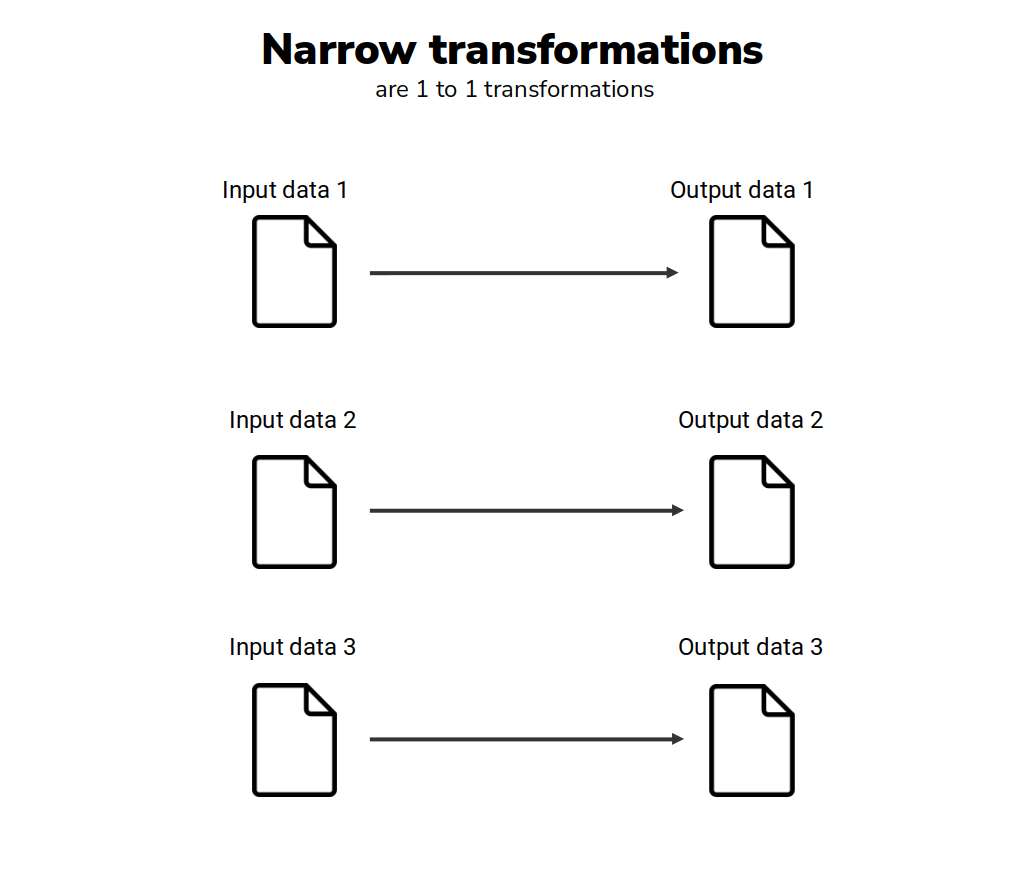
\includegraphics{Chapters/../Figures/narrow-transformations.png}

}

\caption{\label{fig-narrow-transformations}Presenting narrow
transformations}

\end{figure}

In other words, each partition of your input DataFrame will be used
(\emph{separately}) to generate one individual part of the result of
your transformation. As another perspective, you can understand narrow
transformations as those where Spark does not need to read the entire
input DataFrame to generate a single and small piece of your result.

A classic example of narrow transformation is a filter. For example,
suppose you have three students (Anne, Carls and Mike), and that each
one has a bag full of blue, orange and red balls mixed. Now, suppose you
asked them to collect all the red balls of these bags, and combined them
in a single bag.

To do this task, Mike does not need to know what balls are inside of the
bag of Carls or Anne. He just need to collect the red balls that are
solely on his bag. At the end of the task, each student will have a part
of the end result (that is, all the red balls that were in his own bag),
and they just need to combine all these parts to get the total result.

The same thing applies to filters in Spark DataFrames. When you filter
all the rows where the column \texttt{state} is equal to
\texttt{"Alaska"}, Spark will filter all the rows in each partition
separately, and then, will combine all the outputs to get the final
result.

In contrast, wide transformations are the opposite of that. In wide
transformations, Spark needs to use more than 1 partition of the input
DataFrame to generate a small piece of the result.

\begin{figure}

{\centering 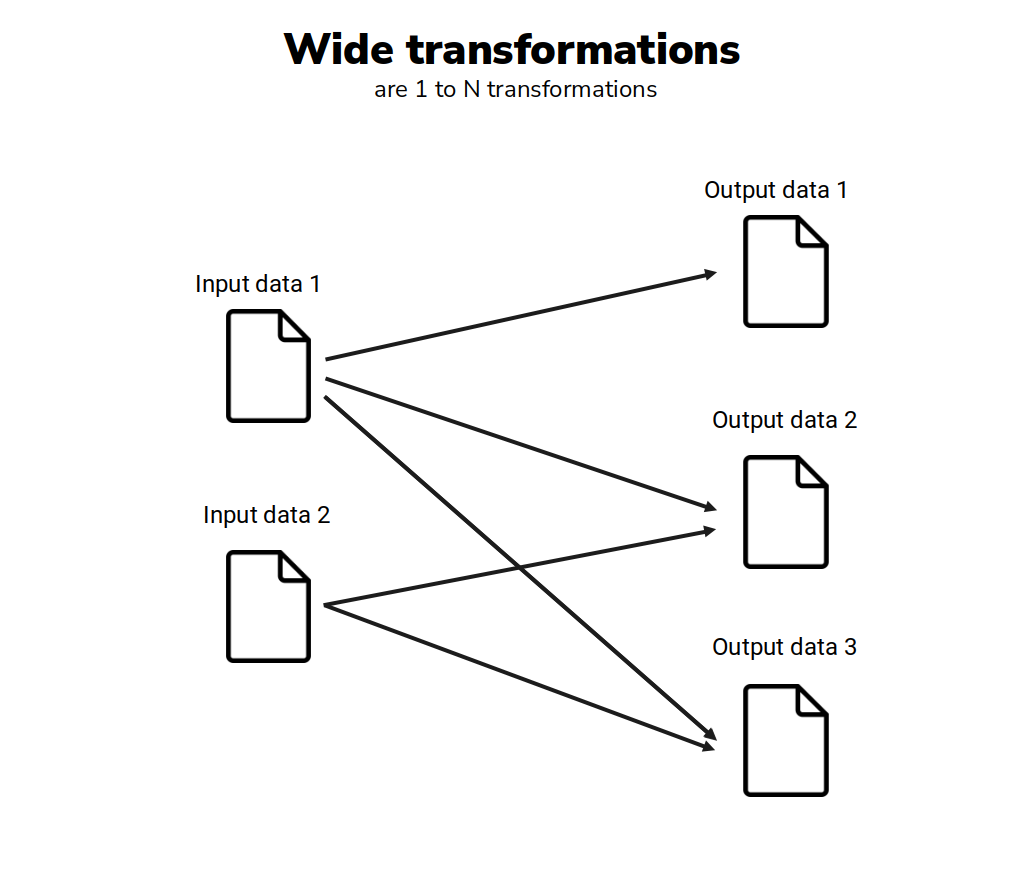
\includegraphics{Chapters/../Figures/wide-transformations.png}

}

\caption{\label{fig-wide-transformations}Presenting wide
transformations}

\end{figure}

When this kind of transformation happens, each worker node of the
cluster needs to share his partition with the others. In other words,
what happens is a partition shuffle. Each worker node sends his
partition to the others, so they can have access to it, while performing
their assigned tasks.

Partition shuffles are a very popular topic in Apache Spark, because
they can be a serious source of inefficiency in your Spark application
(Chambers and Zaharia 2018). In more details, when these shuffles
happens, Spark needs to write data back to the hard disk of the
computer, and this is not a very fast operation. It does not mean that
wide transformations are bad or slow, just that the shuffles they are
producing can be a problem.

A classic example of wide operation is a grouped aggregation. For
example, lets suppose we had a DataFrame with the daily sales of
multiple stores spread across the country, and, we wanted to calculate
the total sales per city/region. To calculate the total sales of a
specific city, like ``São Paulo'', Spark would need to find all the rows
that corresponds to this city, before adding the values, and these rows
can be spread across multiple partitions of the cluster.

\hypertarget{the-transf-dataframe}{%
\section{\texorpdfstring{The \texttt{transf}
DataFrame}{The transf DataFrame}}\label{the-transf-dataframe}}

To demonstrate some of the next examples in this chapter, we will use a
different DataFrame called \texttt{transf}. The data that represents
this DataFrame is freely available as a CSV file. You can download this
CSV at the repository of this book\footnote{\url{https://github.com/pedropark99/Introd-pyspark/tree/main/Data}}.

With the code below, you can import the data from the
\texttt{transf.csv} CSV file, to recreate the \texttt{transf} DataFrame
in your Spark Session:

\begin{Shaded}
\begin{Highlighting}[]
\ImportTok{from}\NormalTok{ pyspark.sql.types }\ImportTok{import}\NormalTok{ StructType, StructField}
\ImportTok{from}\NormalTok{ pyspark.sql.types }\ImportTok{import}\NormalTok{ DoubleType, StringType}
\ImportTok{from}\NormalTok{ pyspark.sql.types }\ImportTok{import}\NormalTok{ LongType, TimestampType, DateType}
\NormalTok{path }\OperatorTok{=} \StringTok{"../Data/transf.csv"}
\NormalTok{schema }\OperatorTok{=}\NormalTok{ StructType([}
\NormalTok{  StructField(}\StringTok{\textquotesingle{}dateTransfer\textquotesingle{}}\NormalTok{, DateType(), }\VariableTok{False}\NormalTok{),}
\NormalTok{  StructField(}\StringTok{\textquotesingle{}datetimeTransfer\textquotesingle{}}\NormalTok{, TimestampType(), }\VariableTok{False}\NormalTok{),}
\NormalTok{  StructField(}\StringTok{\textquotesingle{}clientNumber\textquotesingle{}}\NormalTok{, LongType(), }\VariableTok{False}\NormalTok{),}
\NormalTok{  StructField(}\StringTok{\textquotesingle{}transferValue\textquotesingle{}}\NormalTok{, DoubleType(), }\VariableTok{False}\NormalTok{),}
\NormalTok{  StructField(}\StringTok{\textquotesingle{}transferCurrency\textquotesingle{}}\NormalTok{, StringType(), }\VariableTok{False}\NormalTok{),}
\NormalTok{  StructField(}\StringTok{\textquotesingle{}transferID\textquotesingle{}}\NormalTok{, LongType(), }\VariableTok{False}\NormalTok{),}
\NormalTok{  StructField(}\StringTok{\textquotesingle{}transferLog\textquotesingle{}}\NormalTok{, StringType(), }\VariableTok{False}\NormalTok{),}
\NormalTok{  StructField(}\StringTok{\textquotesingle{}destinationBankNumber\textquotesingle{}}\NormalTok{, LongType(), }\VariableTok{False}\NormalTok{),}
\NormalTok{  StructField(}\StringTok{\textquotesingle{}destinationBankBranch\textquotesingle{}}\NormalTok{, LongType(), }\VariableTok{False}\NormalTok{),}
\NormalTok{  StructField(}\StringTok{\textquotesingle{}destinationBankAccount\textquotesingle{}}\NormalTok{, StringType(), }\VariableTok{False}\NormalTok{)}
\NormalTok{])}

\NormalTok{transf }\OperatorTok{=}\NormalTok{ spark.read}\OperatorTok{\textbackslash{}}
\NormalTok{  .csv(path, schema }\OperatorTok{=}\NormalTok{ schema, sep }\OperatorTok{=} \StringTok{";"}\NormalTok{, header }\OperatorTok{=} \VariableTok{True}\NormalTok{)}
\end{Highlighting}
\end{Shaded}

You could also use the \texttt{pandas} library to read the DataFrame
directly from GitHub, without having to manually download the file:

\begin{Shaded}
\begin{Highlighting}[]
\ImportTok{import}\NormalTok{ pandas }\ImportTok{as}\NormalTok{ pd}
\NormalTok{url }\OperatorTok{=} \StringTok{\textquotesingle{}https://raw.githubusercontent.com/\textquotesingle{}}
\NormalTok{url }\OperatorTok{=}\NormalTok{ url }\OperatorTok{+} \StringTok{\textquotesingle{}pedropark99/Introd{-}pyspark/\textquotesingle{}}
\NormalTok{url }\OperatorTok{=}\NormalTok{ url }\OperatorTok{+} \StringTok{\textquotesingle{}main/Data/transf.csv\textquotesingle{}}

\NormalTok{transf\_pd }\OperatorTok{=}\NormalTok{ pd.read\_csv(}
\NormalTok{  url, sep }\OperatorTok{=} \StringTok{\textquotesingle{};\textquotesingle{}}\NormalTok{,}
\NormalTok{  dtype }\OperatorTok{=} \BuiltInTok{str}\NormalTok{,}
\NormalTok{  keep\_default\_na }\OperatorTok{=} \VariableTok{False}
\NormalTok{)}

\NormalTok{transf\_pd[}\StringTok{\textquotesingle{}transferValue\textquotesingle{}}\NormalTok{] }\OperatorTok{=}\NormalTok{ transf\_pd[}\StringTok{\textquotesingle{}transferValue\textquotesingle{}}\NormalTok{].astype(}\StringTok{\textquotesingle{}float\textquotesingle{}}\NormalTok{)}

\NormalTok{columns\_to\_int }\OperatorTok{=}\NormalTok{ [}
  \StringTok{\textquotesingle{}clientNumber\textquotesingle{}}\NormalTok{,}
  \StringTok{\textquotesingle{}transferID\textquotesingle{}}\NormalTok{,}
  \StringTok{\textquotesingle{}destinationBankNumber\textquotesingle{}}\NormalTok{,}
  \StringTok{\textquotesingle{}destinationBankBranch\textquotesingle{}}
\NormalTok{]}
\ControlFlowTok{for}\NormalTok{ column }\KeywordTok{in}\NormalTok{ columns\_to\_int:}
\NormalTok{  transf\_pd[column] }\OperatorTok{=}\NormalTok{ transf\_pd[column].astype(}\StringTok{\textquotesingle{}int\textquotesingle{}}\NormalTok{)}

\ImportTok{from}\NormalTok{ pyspark.sql }\ImportTok{import}\NormalTok{ SparkSession}
\ImportTok{from}\NormalTok{ pyspark.sql.functions }\ImportTok{import}\NormalTok{ col}
\NormalTok{spark }\OperatorTok{=}\NormalTok{ SparkSession.builder.getOrCreate()}
\NormalTok{transf }\OperatorTok{=}\NormalTok{ spark.createDataFrame(transf\_pd)}\OperatorTok{\textbackslash{}}
\NormalTok{  .withColumn(}\StringTok{\textquotesingle{}dateTransfer\textquotesingle{}}\NormalTok{, col(}\StringTok{\textquotesingle{}dateTransfer\textquotesingle{}}\NormalTok{).cast(}\StringTok{\textquotesingle{}date\textquotesingle{}}\NormalTok{))}\OperatorTok{\textbackslash{}}
\NormalTok{  .withColumn(}\StringTok{\textquotesingle{}datetimeTransfer\textquotesingle{}}\NormalTok{, col(}\StringTok{\textquotesingle{}datetimeTransfer\textquotesingle{}}\NormalTok{).cast(}\StringTok{\textquotesingle{}timestamp\textquotesingle{}}\NormalTok{))}
\end{Highlighting}
\end{Shaded}

This \texttt{transf} DataFrame contains bank transfer records from a
fictitious bank. Before I show you the actual data of this DataFrame, is
useful to give you a quick description of each column that it contains:

\begin{itemize}
\tightlist
\item
  \texttt{dateTransfer}: the date when the transfer occurred;
\item
  \texttt{datetimeTransfer}: the date and time when the transfer
  occurred;
\item
  \texttt{clientNumber} the unique number that identifies a client of
  the bank;
\item
  \texttt{transferValue}: the nominal value that was transferred;
\item
  \texttt{transferCurrency}: the currency of the nominal value
  transferred;
\item
  \texttt{transferID}: an unique ID for the transfer;
\item
  \texttt{transferLog}: store any error message that may have appeared
  during the execution of the transfer;
\item
  \texttt{destinationBankNumber}: the transfer destination bank number;
\item
  \texttt{destinationBankBranch}: the transfer destination branch
  number;
\item
  \texttt{destinationBankAccount}: the transfer destination account
  number;
\end{itemize}

Now, to see the actual data of this DataFrame, we can use the
\texttt{show()} action as usual.

\begin{Shaded}
\begin{Highlighting}[]
\NormalTok{transf.show(}\DecValTok{5}\NormalTok{)}
\end{Highlighting}
\end{Shaded}

\begin{verbatim}
+------------+-------------------+------------+-------------+----------------+----------+-----------+---------------------+---------------------+----------------------+
|dateTransfer|   datetimeTransfer|clientNumber|transferValue|transferCurrency|transferID|transferLog|destinationBankNumber|destinationBankBranch|destinationBankAccount|
+------------+-------------------+------------+-------------+----------------+----------+-----------+---------------------+---------------------+----------------------+
|  2022-12-31|2022-12-31 14:00:24|        5516|      7794.31|          zing ƒ|  20223563|       null|                   33|                 4078|               72424-2|
|  2022-12-31|2022-12-31 10:32:07|        4965|       7919.0|          zing ƒ|  20223562|       null|                  421|                 1979|               36441-5|
|  2022-12-31|2022-12-31 07:37:02|        4608|       5603.0|        dollar $|  20223561|       null|                  666|                 4425|               41323-1|
|  2022-12-31|2022-12-31 07:35:05|        1121|      4365.22|        dollar $|  20223560|       null|                  666|                 2400|               74120-4|
|  2022-12-31|2022-12-31 02:53:44|        1121|       4620.0|        dollar $|  20223559|       null|                  421|                 1100|               39830-0|
+------------+-------------------+------------+-------------+----------------+----------+-----------+---------------------+---------------------+----------------------+
only showing top 5 rows
\end{verbatim}

\hypertarget{filtering-rows-of-your-dataframe}{%
\section{Filtering rows of your
DataFrame}\label{filtering-rows-of-your-dataframe}}

To filter specific rows of a DataFrame, \texttt{pyspark} offers two
equivalent DataFrame methods called \texttt{where()} and
\texttt{filter()}. In other words, they both do the same thing, and work
in the same way. These methods receives as input a logical expression
that translates what you want to filter.

As a first example, lets suppose you wanted to inspect all the rows from
the \texttt{transf} DataFrame where \texttt{transferValue} is less than
1000. To do so, you can use the following code:

\begin{Shaded}
\begin{Highlighting}[]
\NormalTok{transf}\OperatorTok{\textbackslash{}}
\NormalTok{  .}\BuiltInTok{filter}\NormalTok{(}\StringTok{"transferValue \textless{} 1000"}\NormalTok{)}\OperatorTok{\textbackslash{}}
\NormalTok{  .show(}\DecValTok{5}\NormalTok{)}
\end{Highlighting}
\end{Shaded}

\begin{verbatim}
+------------+-------------------+------------+-------------+----------------+----------+-----------+---------------------+---------------------+----------------------+
|dateTransfer|   datetimeTransfer|clientNumber|transferValue|transferCurrency|transferID|transferLog|destinationBankNumber|destinationBankBranch|destinationBankAccount|
+------------+-------------------+------------+-------------+----------------+----------+-----------+---------------------+---------------------+----------------------+
|  2022-12-18|2022-12-18 08:45:30|        1297|       142.66|        dollar $|  20223467|       null|                  421|                 5420|               43088-1|
|  2022-12-13|2022-12-13 20:44:23|        5516|       992.15|        dollar $|  20223442|       null|                   33|                 5420|               41609-8|
|  2022-11-24|2022-11-24 20:01:39|        1945|       174.64|        dollar $|  20223319|       null|                  421|                 2400|               34025-8|
|  2022-11-07|2022-11-07 16:35:57|        4862|       570.69|        dollar $|  20223212|       null|                  290|                 5420|               51165-3|
|  2022-11-04|2022-11-04 20:00:34|        1297|        854.0|        dollar $|  20223194|       null|                  421|                 4078|               43478-6|
+------------+-------------------+------------+-------------+----------------+----------+-----------+---------------------+---------------------+----------------------+
only showing top 5 rows
\end{verbatim}

Writing simple SQL logical expression inside a string is the most easy
and ``clean'' way to create a filter expression in \texttt{pyspark}.
However, you could also write the same exact expression in a more
``pythonic'' way, using the \texttt{col()} function from
\texttt{pyspark.sql.functions} module.

\begin{Shaded}
\begin{Highlighting}[]
\ImportTok{from}\NormalTok{ pyspark.sql.functions }\ImportTok{import}\NormalTok{ col}

\NormalTok{transf}\OperatorTok{\textbackslash{}}
\NormalTok{  .}\BuiltInTok{filter}\NormalTok{(col(}\StringTok{"transferValue"}\NormalTok{) }\OperatorTok{\textless{}} \DecValTok{1000}\NormalTok{)}\OperatorTok{\textbackslash{}}
\NormalTok{  .show(}\DecValTok{5}\NormalTok{)}
\end{Highlighting}
\end{Shaded}

\begin{verbatim}
+------------+-------------------+------------+-------------+----------------+----------+-----------+---------------------+---------------------+----------------------+
|dateTransfer|   datetimeTransfer|clientNumber|transferValue|transferCurrency|transferID|transferLog|destinationBankNumber|destinationBankBranch|destinationBankAccount|
+------------+-------------------+------------+-------------+----------------+----------+-----------+---------------------+---------------------+----------------------+
|  2022-12-18|2022-12-18 08:45:30|        1297|       142.66|        dollar $|  20223467|       null|                  421|                 5420|               43088-1|
|  2022-12-13|2022-12-13 20:44:23|        5516|       992.15|        dollar $|  20223442|       null|                   33|                 5420|               41609-8|
|  2022-11-24|2022-11-24 20:01:39|        1945|       174.64|        dollar $|  20223319|       null|                  421|                 2400|               34025-8|
|  2022-11-07|2022-11-07 16:35:57|        4862|       570.69|        dollar $|  20223212|       null|                  290|                 5420|               51165-3|
|  2022-11-04|2022-11-04 20:00:34|        1297|        854.0|        dollar $|  20223194|       null|                  421|                 4078|               43478-6|
+------------+-------------------+------------+-------------+----------------+----------+-----------+---------------------+---------------------+----------------------+
only showing top 5 rows
\end{verbatim}

You still have a more verbose alternative, that does not require the
\texttt{col()} function. With this method, you refer to the specific
column using the dot operator (\texttt{.}), like in the example below:

\begin{Shaded}
\begin{Highlighting}[]
\CommentTok{\# This will give you the exact}
\CommentTok{\# same result of the examples above}
\NormalTok{transf}\OperatorTok{\textbackslash{}}
\NormalTok{  .}\BuiltInTok{filter}\NormalTok{(transf.transferValue }\OperatorTok{\textless{}} \DecValTok{1000}\NormalTok{)}
\end{Highlighting}
\end{Shaded}

\hypertarget{logical-operators-available}{%
\subsection{Logical operators
available}\label{logical-operators-available}}

As we saw in the previous section, there are two ways to write logical
expressions in \texttt{pyspark}: 1) write a SQL logical expression
inside a string; 2) or, write a python logical expression using the
\texttt{col()} function.

If you choose to write a SQL logical expressions in a string, you need
to use the logical operators of SQL in your expression (not the logical
operators of python). In the other hand, if you choose to write in the
``python'' way, then, you need to use the logical operators of python
instead.

The logical operators of SQL are described in the table below:

\hypertarget{tbl-logical-operators-sql}{}
\begin{longtable}[]{@{}
  >{\raggedright\arraybackslash}p{(\columnwidth - 4\tabcolsep) * \real{0.1124}}
  >{\raggedright\arraybackslash}p{(\columnwidth - 4\tabcolsep) * \real{0.2472}}
  >{\raggedright\arraybackslash}p{(\columnwidth - 4\tabcolsep) * \real{0.6404}}@{}}
\caption{\label{tbl-logical-operators-sql}List of logical operators of
SQL}\tabularnewline
\toprule()
\begin{minipage}[b]{\linewidth}\raggedright
Operator
\end{minipage} & \begin{minipage}[b]{\linewidth}\raggedright
Example of expression
\end{minipage} & \begin{minipage}[b]{\linewidth}\raggedright
Meaning of the expression
\end{minipage} \\
\midrule()
\endfirsthead
\toprule()
\begin{minipage}[b]{\linewidth}\raggedright
Operator
\end{minipage} & \begin{minipage}[b]{\linewidth}\raggedright
Example of expression
\end{minipage} & \begin{minipage}[b]{\linewidth}\raggedright
Meaning of the expression
\end{minipage} \\
\midrule()
\endhead
\textless{} & \texttt{x\ \textless{}\ y} & is \texttt{x} less than
\texttt{y}? \\
\textgreater{} & \texttt{x\ \textgreater{}\ y} & is \texttt{x} greater
than \texttt{y}? \\
\textless= & \texttt{x\ \textless{}=\ y} & is \texttt{x} less than or
equal to \texttt{y}? \\
\textgreater= & \texttt{x\ \textgreater{}=\ y} & is \texttt{x} greater
than or equal to \texttt{y}? \\
== & \texttt{x\ ==\ y} & is \texttt{x} equal to \texttt{y}? \\
!= & \texttt{x\ !=\ y} & is \texttt{x} not equal to \texttt{y}? \\
in & \texttt{x\ in\ y} & is \texttt{x} one of the values listed in
\texttt{y}? \\
and & \texttt{x\ and\ y} & both logical expressions \texttt{x} and
\texttt{y} are true? \\
or & \texttt{x\ or\ y} & at least one of logical expressions \texttt{x}
and \texttt{y} are true? \\
not & \texttt{not\ x} & is the logical expression \texttt{x} not
true? \\
\bottomrule()
\end{longtable}

And, the logical operators of python are described in the table below:

\hypertarget{tbl-logical-operators-python}{}
\begin{longtable}[]{@{}
  >{\raggedright\arraybackslash}p{(\columnwidth - 4\tabcolsep) * \real{0.1124}}
  >{\raggedright\arraybackslash}p{(\columnwidth - 4\tabcolsep) * \real{0.2472}}
  >{\raggedright\arraybackslash}p{(\columnwidth - 4\tabcolsep) * \real{0.6404}}@{}}
\caption{\label{tbl-logical-operators-python}List of logical operators
of python}\tabularnewline
\toprule()
\begin{minipage}[b]{\linewidth}\raggedright
Operator
\end{minipage} & \begin{minipage}[b]{\linewidth}\raggedright
Example of expression
\end{minipage} & \begin{minipage}[b]{\linewidth}\raggedright
Meaning of the expression
\end{minipage} \\
\midrule()
\endfirsthead
\toprule()
\begin{minipage}[b]{\linewidth}\raggedright
Operator
\end{minipage} & \begin{minipage}[b]{\linewidth}\raggedright
Example of expression
\end{minipage} & \begin{minipage}[b]{\linewidth}\raggedright
Meaning of the expression
\end{minipage} \\
\midrule()
\endhead
\textless{} & \texttt{x\ \textless{}\ y} & is \texttt{x} less than
\texttt{y}? \\
\textgreater{} & \texttt{x\ \textgreater{}\ y} & is \texttt{x} greater
than \texttt{y}? \\
\textless= & \texttt{x\ \textless{}=\ y} & is \texttt{x} less than or
equal to \texttt{y}? \\
\textgreater= & \texttt{x\ \textgreater{}=\ y} & is \texttt{x} greater
than or equal to \texttt{y}? \\
== & \texttt{x\ ==\ y} & is \texttt{x} equal to \texttt{y}? \\
!= & \texttt{x\ !=\ y} & is \texttt{x} not equal to \texttt{y}? \\
\& & \texttt{x\ \&\ y} & both logical expressions \texttt{x} and
\texttt{y} are true? \\
\textbar{} & \texttt{x\ \textbar{}\ y} & at least one of logical
expressions \texttt{x} and \texttt{y} are true? \\
\textasciitilde{} & \texttt{\textasciitilde{}x} & is the logical
expression \texttt{x} not true? \\
\bottomrule()
\end{longtable}

\hypertarget{connecting-multiple-logical-expressions}{%
\subsection{Connecting multiple logical
expressions}\label{connecting-multiple-logical-expressions}}

Sometimes, you need to write more complex logical expressions to
correctly describe the rows you are interested in. That is, when you
combine multiple logical expressions together.

As an example, lets suppose you wanted all the rows in \texttt{transf}
DataFrame from client of number 1297 where the transfer value is smaller
than 1000, and the date of the transfer is after 20 of February 2022.
These conditions are dependent, that is, they are connected to each
other (the client number, the transfer value and the date of the
transfer). That is why I used the \texttt{and} keyword between each
condition in the example below (i.e.~to connect these three conditions
together).

\begin{Shaded}
\begin{Highlighting}[]
\NormalTok{condition }\OperatorTok{=} \StringTok{\textquotesingle{}\textquotesingle{}\textquotesingle{}}
\StringTok{  transferValue \textless{} 1000}
\StringTok{  and clientNumber == 1297 }
\StringTok{  and dateTransfer \textgreater{} \textquotesingle{}2022{-}02{-}20\textquotesingle{}}
\StringTok{\textquotesingle{}\textquotesingle{}\textquotesingle{}}

\NormalTok{transf}\OperatorTok{\textbackslash{}}
\NormalTok{  .}\BuiltInTok{filter}\NormalTok{(condition)}\OperatorTok{\textbackslash{}}
\NormalTok{  .show()}
\end{Highlighting}
\end{Shaded}

\begin{verbatim}
+------------+-------------------+------------+-------------+----------------+----------+-----------+---------------------+---------------------+----------------------+
|dateTransfer|   datetimeTransfer|clientNumber|transferValue|transferCurrency|transferID|transferLog|destinationBankNumber|destinationBankBranch|destinationBankAccount|
+------------+-------------------+------------+-------------+----------------+----------+-----------+---------------------+---------------------+----------------------+
|  2022-12-18|2022-12-18 08:45:30|        1297|       142.66|        dollar $|  20223467|       null|                  421|                 5420|               43088-1|
|  2022-11-04|2022-11-04 20:00:34|        1297|        854.0|        dollar $|  20223194|       null|                  421|                 4078|               43478-6|
|  2022-02-27|2022-02-27 13:27:44|        1297|       697.21|        dollar $|  20221505|       null|                  421|                 1100|               60414-7|
+------------+-------------------+------------+-------------+----------------+----------+-----------+---------------------+---------------------+----------------------+
\end{verbatim}

I could translate this logical expression into the ``pythonic'' way
(using the \texttt{col()} function). However, I would have to surround
each individual expression by parentheses, and, use the \texttt{\&}
operator to substitute the \texttt{and} keyword.

\begin{Shaded}
\begin{Highlighting}[]
\NormalTok{transf}\OperatorTok{\textbackslash{}}
\NormalTok{  .}\BuiltInTok{filter}\NormalTok{(}
\NormalTok{    (col(}\StringTok{\textquotesingle{}transferValue\textquotesingle{}}\NormalTok{) }\OperatorTok{\textless{}} \DecValTok{1000}\NormalTok{) }\OperatorTok{\&}
\NormalTok{    (col(}\StringTok{\textquotesingle{}clientNumber\textquotesingle{}}\NormalTok{) }\OperatorTok{==} \DecValTok{1297}\NormalTok{) }\OperatorTok{\&}
\NormalTok{    (col(}\StringTok{\textquotesingle{}dateTransfer\textquotesingle{}}\NormalTok{) }\OperatorTok{\textgreater{}} \StringTok{\textquotesingle{}2022{-}02{-}20\textquotesingle{}}\NormalTok{)}
\NormalTok{  )}\OperatorTok{\textbackslash{}}
\NormalTok{  .show()}
\end{Highlighting}
\end{Shaded}

\begin{verbatim}
+------------+-------------------+------------+-------------+----------------+----------+-----------+---------------------+---------------------+----------------------+
|dateTransfer|   datetimeTransfer|clientNumber|transferValue|transferCurrency|transferID|transferLog|destinationBankNumber|destinationBankBranch|destinationBankAccount|
+------------+-------------------+------------+-------------+----------------+----------+-----------+---------------------+---------------------+----------------------+
|  2022-12-18|2022-12-18 08:45:30|        1297|       142.66|        dollar $|  20223467|       null|                  421|                 5420|               43088-1|
|  2022-11-04|2022-11-04 20:00:34|        1297|        854.0|        dollar $|  20223194|       null|                  421|                 4078|               43478-6|
|  2022-02-27|2022-02-27 13:27:44|        1297|       697.21|        dollar $|  20221505|       null|                  421|                 1100|               60414-7|
+------------+-------------------+------------+-------------+----------------+----------+-----------+---------------------+---------------------+----------------------+
\end{verbatim}

This a \textbf{very important detail}, because it is very easy to
forget. When building your complex logical expressions in the ``python''
way, always \textbf{remember to surround each expression by a pair of
parentheses}. Otherwise, you will get a very confusing and useless error
message, like this:

\begin{Shaded}
\begin{Highlighting}[]
\NormalTok{transf}\OperatorTok{\textbackslash{}}
\NormalTok{  .}\BuiltInTok{filter}\NormalTok{(}
\NormalTok{    col(}\StringTok{\textquotesingle{}transferValue\textquotesingle{}}\NormalTok{) }\OperatorTok{\textless{}} \DecValTok{1000} \OperatorTok{\&}
\NormalTok{    col(}\StringTok{\textquotesingle{}clientNumber\textquotesingle{}}\NormalTok{) }\OperatorTok{==} \DecValTok{1297} \OperatorTok{\&}
\NormalTok{    col(}\StringTok{\textquotesingle{}dateTransfer\textquotesingle{}}\NormalTok{) }\OperatorTok{\textgreater{}} \StringTok{\textquotesingle{}2022{-}02{-}20\textquotesingle{}}
\NormalTok{  )}\OperatorTok{\textbackslash{}}
\NormalTok{  .show(}\DecValTok{5}\NormalTok{)}
\end{Highlighting}
\end{Shaded}

\begin{verbatim}
Py4JError: An error occurred while calling o216.and. Trace:
py4j.Py4JException: Method and([class java.lang.Integer]) does not exist
    at py4j.reflection.ReflectionEngine.getMethod(ReflectionEngine.java:318)
    at py4j.reflection.ReflectionEngine.getMethod(ReflectionEngine.java:326)
    at py4j.Gateway.invoke(Gateway.java:274)
    at py4j.commands.AbstractCommand.invokeMethod(AbstractCommand.java:132)
    at py4j.commands.CallCommand.execute(CallCommand.java:79)
    at py4j.ClientServerConnection.waitForCommands(ClientServerConnection.java:182)
    at py4j.ClientServerConnection.run(ClientServerConnection.java:106)
    at java.base/java.lang.Thread.run(Thread.java:829)
\end{verbatim}

In the above examples, we have logical expressions that are dependent on
each other. But, lets suppose these conditions were independent. In this
case, we would use the \texttt{or} keyword, instead of \texttt{and}.
Now, Spark will look for every row of \texttt{transf} where
\texttt{transferValue} is smaller than 1000, or, \texttt{clientNumber}
is equal to 1297, or, \texttt{dateTransfer} is greater than 20 of
February 2022.

\begin{Shaded}
\begin{Highlighting}[]
\NormalTok{condition }\OperatorTok{=} \StringTok{\textquotesingle{}\textquotesingle{}\textquotesingle{}}
\StringTok{  transferValue \textless{} 1000}
\StringTok{  or clientNumber == 1297 }
\StringTok{  or dateTransfer \textgreater{} \textquotesingle{}2022{-}02{-}20\textquotesingle{}}
\StringTok{\textquotesingle{}\textquotesingle{}\textquotesingle{}}

\NormalTok{transf}\OperatorTok{\textbackslash{}}
\NormalTok{  .}\BuiltInTok{filter}\NormalTok{(condition)}\OperatorTok{\textbackslash{}}
\NormalTok{  .show(}\DecValTok{5}\NormalTok{)}
\end{Highlighting}
\end{Shaded}

\begin{verbatim}
+------------+-------------------+------------+-------------+----------------+----------+-----------+---------------------+---------------------+----------------------+
|dateTransfer|   datetimeTransfer|clientNumber|transferValue|transferCurrency|transferID|transferLog|destinationBankNumber|destinationBankBranch|destinationBankAccount|
+------------+-------------------+------------+-------------+----------------+----------+-----------+---------------------+---------------------+----------------------+
|  2022-12-31|2022-12-31 14:00:24|        5516|      7794.31|          zing ƒ|  20223563|       null|                   33|                 4078|               72424-2|
|  2022-12-31|2022-12-31 10:32:07|        4965|       7919.0|          zing ƒ|  20223562|       null|                  421|                 1979|               36441-5|
|  2022-12-31|2022-12-31 07:37:02|        4608|       5603.0|        dollar $|  20223561|       null|                  666|                 4425|               41323-1|
|  2022-12-31|2022-12-31 07:35:05|        1121|      4365.22|        dollar $|  20223560|       null|                  666|                 2400|               74120-4|
|  2022-12-31|2022-12-31 02:53:44|        1121|       4620.0|        dollar $|  20223559|       null|                  421|                 1100|               39830-0|
+------------+-------------------+------------+-------------+----------------+----------+-----------+---------------------+---------------------+----------------------+
only showing top 5 rows
\end{verbatim}

To translate this expression into the pythonic way, we have to
substitute the \texttt{or} keyword by the \texttt{\textbar{}} operator,
and surround each expression by parentheses again:

\begin{Shaded}
\begin{Highlighting}[]
\NormalTok{transf}\OperatorTok{\textbackslash{}}
\NormalTok{  .}\BuiltInTok{filter}\NormalTok{(}
\NormalTok{    (col(}\StringTok{\textquotesingle{}transferValue\textquotesingle{}}\NormalTok{) }\OperatorTok{\textless{}} \DecValTok{1000}\NormalTok{) }\OperatorTok{|}
\NormalTok{    (col(}\StringTok{\textquotesingle{}clientNumber\textquotesingle{}}\NormalTok{) }\OperatorTok{==} \DecValTok{1297}\NormalTok{) }\OperatorTok{|}
\NormalTok{    (col(}\StringTok{\textquotesingle{}dateTransfer\textquotesingle{}}\NormalTok{) }\OperatorTok{\textgreater{}} \StringTok{\textquotesingle{}2022{-}02{-}20\textquotesingle{}}\NormalTok{)}
\NormalTok{  )}\OperatorTok{\textbackslash{}}
\NormalTok{  .show(}\DecValTok{5}\NormalTok{)}
\end{Highlighting}
\end{Shaded}

\begin{verbatim}
+------------+-------------------+------------+-------------+----------------+----------+-----------+---------------------+---------------------+----------------------+
|dateTransfer|   datetimeTransfer|clientNumber|transferValue|transferCurrency|transferID|transferLog|destinationBankNumber|destinationBankBranch|destinationBankAccount|
+------------+-------------------+------------+-------------+----------------+----------+-----------+---------------------+---------------------+----------------------+
|  2022-12-31|2022-12-31 14:00:24|        5516|      7794.31|          zing ƒ|  20223563|       null|                   33|                 4078|               72424-2|
|  2022-12-31|2022-12-31 10:32:07|        4965|       7919.0|          zing ƒ|  20223562|       null|                  421|                 1979|               36441-5|
|  2022-12-31|2022-12-31 07:37:02|        4608|       5603.0|        dollar $|  20223561|       null|                  666|                 4425|               41323-1|
|  2022-12-31|2022-12-31 07:35:05|        1121|      4365.22|        dollar $|  20223560|       null|                  666|                 2400|               74120-4|
|  2022-12-31|2022-12-31 02:53:44|        1121|       4620.0|        dollar $|  20223559|       null|                  421|                 1100|               39830-0|
+------------+-------------------+------------+-------------+----------------+----------+-----------+---------------------+---------------------+----------------------+
only showing top 5 rows
\end{verbatim}

You can also increase the complexity of your logical expressions by
mixing dependent expressions with independent expressions. For example,
to filter all the rows where \texttt{dateTransfer} is greater than or
equal to 01 of October 2022, and \texttt{clientNumber} is either 2727 or
5188, you would have the following code:

\begin{Shaded}
\begin{Highlighting}[]
\NormalTok{condition }\OperatorTok{=} \StringTok{\textquotesingle{}\textquotesingle{}\textquotesingle{}}
\StringTok{  (clientNumber == 2727 or clientNumber == 5188)}
\StringTok{  and dateTransfer \textgreater{}= \textquotesingle{}2022{-}10{-}01\textquotesingle{}}
\StringTok{\textquotesingle{}\textquotesingle{}\textquotesingle{}}

\NormalTok{transf}\OperatorTok{\textbackslash{}}
\NormalTok{  .}\BuiltInTok{filter}\NormalTok{(condition)}\OperatorTok{\textbackslash{}}
\NormalTok{  .show(}\DecValTok{5}\NormalTok{)}
\end{Highlighting}
\end{Shaded}

\begin{verbatim}
+------------+-------------------+------------+-------------+----------------+----------+-----------+---------------------+---------------------+----------------------+
|dateTransfer|   datetimeTransfer|clientNumber|transferValue|transferCurrency|transferID|transferLog|destinationBankNumber|destinationBankBranch|destinationBankAccount|
+------------+-------------------+------------+-------------+----------------+----------+-----------+---------------------+---------------------+----------------------+
|  2022-12-29|2022-12-29 10:22:02|        2727|      4666.25|          euro €|  20223541|       null|                   33|                 5420|               83070-8|
|  2022-12-27|2022-12-27 03:58:25|        5188|      7821.69|        dollar $|  20223522|       null|                   33|                 4078|               46571-3|
|  2022-12-26|2022-12-25 23:45:02|        2727|      3261.73| british pound £|  20223515|       null|                  421|                 6317|               66040-9|
|  2022-12-23|2022-12-23 05:32:49|        2727|       8042.0|        dollar $|  20223496|       null|                  290|                 5420|               37759-7|
|  2022-12-22|2022-12-22 06:02:47|        5188|      8175.67|        dollar $|  20223490|       null|                  666|                 8800|               42657-8|
+------------+-------------------+------------+-------------+----------------+----------+-----------+---------------------+---------------------+----------------------+
only showing top 5 rows
\end{verbatim}

If you investigate the above condition carefully, maybe, you will
identify that this condition could be rewritten in a simpler format, by
using the \texttt{in} keyword. This way, Spark will look for all the
rows where \texttt{clientNumber} is equal to one of the listed values
(2727 or 5188), and, that \texttt{dateTransfer} is greater than or equal
to 01 of October 2022.

\begin{Shaded}
\begin{Highlighting}[]
\NormalTok{condition }\OperatorTok{=} \StringTok{\textquotesingle{}\textquotesingle{}\textquotesingle{}}
\StringTok{  clientNumber in (2727, 5188)}
\StringTok{  and dateTransfer \textgreater{}= \textquotesingle{}2022{-}10{-}01\textquotesingle{}}
\StringTok{\textquotesingle{}\textquotesingle{}\textquotesingle{}}

\NormalTok{transf}\OperatorTok{\textbackslash{}}
\NormalTok{  .}\BuiltInTok{filter}\NormalTok{(condition)}\OperatorTok{\textbackslash{}}
\NormalTok{  .show(}\DecValTok{5}\NormalTok{)}
\end{Highlighting}
\end{Shaded}

\begin{verbatim}
+------------+-------------------+------------+-------------+----------------+----------+-----------+---------------------+---------------------+----------------------+
|dateTransfer|   datetimeTransfer|clientNumber|transferValue|transferCurrency|transferID|transferLog|destinationBankNumber|destinationBankBranch|destinationBankAccount|
+------------+-------------------+------------+-------------+----------------+----------+-----------+---------------------+---------------------+----------------------+
|  2022-12-29|2022-12-29 10:22:02|        2727|      4666.25|          euro €|  20223541|       null|                   33|                 5420|               83070-8|
|  2022-12-27|2022-12-27 03:58:25|        5188|      7821.69|        dollar $|  20223522|       null|                   33|                 4078|               46571-3|
|  2022-12-26|2022-12-25 23:45:02|        2727|      3261.73| british pound £|  20223515|       null|                  421|                 6317|               66040-9|
|  2022-12-23|2022-12-23 05:32:49|        2727|       8042.0|        dollar $|  20223496|       null|                  290|                 5420|               37759-7|
|  2022-12-22|2022-12-22 06:02:47|        5188|      8175.67|        dollar $|  20223490|       null|                  666|                 8800|               42657-8|
+------------+-------------------+------------+-------------+----------------+----------+-----------+---------------------+---------------------+----------------------+
only showing top 5 rows
\end{verbatim}

\hypertarget{translating-the-in-keyword-to-the-pythonic-way}{%
\subsection{\texorpdfstring{Translating the \texttt{in} keyword to the
pythonic
way}{Translating the in keyword to the pythonic way}}\label{translating-the-in-keyword-to-the-pythonic-way}}

Python does have a \texttt{in} keyword just like SQL, but, this keyword
does not work as expected in \texttt{pyspark}. To write a logical
expression, using the pythonic way, that filters the rows where a column
is equal to one of the listed values, you can use the \texttt{isin()}
method.

This method belongs to the \texttt{Column} class, so, you should always
use \texttt{isin()} after a column name or a \texttt{col()} function. In
the example below, we are filtering the rows where
\texttt{destinationBankNumber} is 290 or 666:

\begin{Shaded}
\begin{Highlighting}[]
\NormalTok{transf}\OperatorTok{\textbackslash{}}
\NormalTok{  .}\BuiltInTok{filter}\NormalTok{(col(}\StringTok{\textquotesingle{}destinationBankNumber\textquotesingle{}}\NormalTok{).isin(}\DecValTok{290}\NormalTok{, }\DecValTok{666}\NormalTok{))}\OperatorTok{\textbackslash{}}
\NormalTok{  .show(}\DecValTok{5}\NormalTok{)}
\end{Highlighting}
\end{Shaded}

\begin{verbatim}
+------------+-------------------+------------+-------------+----------------+----------+-----------+---------------------+---------------------+----------------------+
|dateTransfer|   datetimeTransfer|clientNumber|transferValue|transferCurrency|transferID|transferLog|destinationBankNumber|destinationBankBranch|destinationBankAccount|
+------------+-------------------+------------+-------------+----------------+----------+-----------+---------------------+---------------------+----------------------+
|  2022-12-31|2022-12-31 07:37:02|        4608|       5603.0|        dollar $|  20223561|       null|                  666|                 4425|               41323-1|
|  2022-12-31|2022-12-31 07:35:05|        1121|      4365.22|        dollar $|  20223560|       null|                  666|                 2400|               74120-4|
|  2022-12-31|2022-12-31 02:44:46|        1121|       7158.0|          zing ƒ|  20223558|       null|                  290|                 1100|               35424-4|
|  2022-12-31|2022-12-31 01:02:06|        4862|       6714.0|        dollar $|  20223557|       null|                  666|                 1002|               71839-1|
|  2022-12-31|2022-12-31 00:48:47|        3294|     10882.52|        dollar $|  20223556|       null|                  666|                 2231|               50190-5|
+------------+-------------------+------------+-------------+----------------+----------+-----------+---------------------+---------------------+----------------------+
only showing top 5 rows
\end{verbatim}

\hypertarget{negating-logical-conditions}{%
\subsection{Negating logical
conditions}\label{negating-logical-conditions}}

In some cases, is easier to describe what rows you \textbf{do not want}
in your filter. That is, you want to negate (or invert) your logical
expression. For this, SQL provides the \texttt{not} keyword, that you
place before the logical expression you want to negate.

For example, we can filter all the rows of \texttt{transf} where
\texttt{clientNumber} is not equal to 3284. Remember, the methods
\texttt{filter()} and \texttt{where()} are equivalents or synonymous
(they both mean the same thing).

\begin{Shaded}
\begin{Highlighting}[]
\NormalTok{condition }\OperatorTok{=} \StringTok{\textquotesingle{}\textquotesingle{}\textquotesingle{}}
\StringTok{  not clientNumber == 3284}
\StringTok{\textquotesingle{}\textquotesingle{}\textquotesingle{}}

\NormalTok{transf}\OperatorTok{\textbackslash{}}
\NormalTok{  .where(condition)}\OperatorTok{\textbackslash{}}
\NormalTok{  .show(}\DecValTok{5}\NormalTok{)}
\end{Highlighting}
\end{Shaded}

\begin{verbatim}
+------------+-------------------+------------+-------------+----------------+----------+-----------+---------------------+---------------------+----------------------+
|dateTransfer|   datetimeTransfer|clientNumber|transferValue|transferCurrency|transferID|transferLog|destinationBankNumber|destinationBankBranch|destinationBankAccount|
+------------+-------------------+------------+-------------+----------------+----------+-----------+---------------------+---------------------+----------------------+
|  2022-12-31|2022-12-31 14:00:24|        5516|      7794.31|          zing ƒ|  20223563|       null|                   33|                 4078|               72424-2|
|  2022-12-31|2022-12-31 10:32:07|        4965|       7919.0|          zing ƒ|  20223562|       null|                  421|                 1979|               36441-5|
|  2022-12-31|2022-12-31 07:37:02|        4608|       5603.0|        dollar $|  20223561|       null|                  666|                 4425|               41323-1|
|  2022-12-31|2022-12-31 07:35:05|        1121|      4365.22|        dollar $|  20223560|       null|                  666|                 2400|               74120-4|
|  2022-12-31|2022-12-31 02:53:44|        1121|       4620.0|        dollar $|  20223559|       null|                  421|                 1100|               39830-0|
+------------+-------------------+------------+-------------+----------------+----------+-----------+---------------------+---------------------+----------------------+
only showing top 5 rows
\end{verbatim}

To translate this expression to the pythonic way, we use the
\texttt{\textasciitilde{}} operator. However, because we are negating
the logical expression as a whole, is important to surround the entire
expression with parentheses.

\begin{Shaded}
\begin{Highlighting}[]
\NormalTok{transf}\OperatorTok{\textbackslash{}}
\NormalTok{  .where(}\OperatorTok{\textasciitilde{}}\NormalTok{(col(}\StringTok{\textquotesingle{}clientNumber\textquotesingle{}}\NormalTok{) }\OperatorTok{==} \DecValTok{3284}\NormalTok{))}\OperatorTok{\textbackslash{}}
\NormalTok{  .show(}\DecValTok{5}\NormalTok{)}
\end{Highlighting}
\end{Shaded}

\begin{verbatim}
+------------+-------------------+------------+-------------+----------------+----------+-----------+---------------------+---------------------+----------------------+
|dateTransfer|   datetimeTransfer|clientNumber|transferValue|transferCurrency|transferID|transferLog|destinationBankNumber|destinationBankBranch|destinationBankAccount|
+------------+-------------------+------------+-------------+----------------+----------+-----------+---------------------+---------------------+----------------------+
|  2022-12-31|2022-12-31 14:00:24|        5516|      7794.31|          zing ƒ|  20223563|       null|                   33|                 4078|               72424-2|
|  2022-12-31|2022-12-31 10:32:07|        4965|       7919.0|          zing ƒ|  20223562|       null|                  421|                 1979|               36441-5|
|  2022-12-31|2022-12-31 07:37:02|        4608|       5603.0|        dollar $|  20223561|       null|                  666|                 4425|               41323-1|
|  2022-12-31|2022-12-31 07:35:05|        1121|      4365.22|        dollar $|  20223560|       null|                  666|                 2400|               74120-4|
|  2022-12-31|2022-12-31 02:53:44|        1121|       4620.0|        dollar $|  20223559|       null|                  421|                 1100|               39830-0|
+------------+-------------------+------------+-------------+----------------+----------+-----------+---------------------+---------------------+----------------------+
only showing top 5 rows
\end{verbatim}

If you forget to add the parentheses, Spark will think you are negating
just the column
(e.g.~\texttt{\textasciitilde{}col(\textquotesingle{}clientNumber\textquotesingle{})}),
and not the entire expression. That would not make sense, and, as a
result, Spark would throw an error:

\begin{Shaded}
\begin{Highlighting}[]
\NormalTok{transf}\OperatorTok{\textbackslash{}}
\NormalTok{  .where(}\OperatorTok{\textasciitilde{}}\NormalTok{col(}\StringTok{\textquotesingle{}clientNumber\textquotesingle{}}\NormalTok{) }\OperatorTok{==} \DecValTok{3284}\NormalTok{)}\OperatorTok{\textbackslash{}}
\NormalTok{  .show(}\DecValTok{5}\NormalTok{)}
\end{Highlighting}
\end{Shaded}

\begin{verbatim}
AnalysisException: cannot resolve '(NOT clientNumber)' due to data type mismatch: argument 1 requires boolean type, however, 'clientNumber' is of bigint type.;
'Filter (NOT clientNumber#210L = 3284)
\end{verbatim}

Because the \texttt{\textasciitilde{}} operator is a little discrete and
can go unnoticed, I sometimes use a different approach to negate my
logical expressions. I make the entire expression equal to
\texttt{False}. This way, I get all the rows where that particular
expression is \texttt{False}. This makes my intention more visible in
the code, but, is harder to write it.

\begin{Shaded}
\begin{Highlighting}[]
\CommentTok{\# Filter all the rows where \textasciigrave{}clientNumber\textasciigrave{} is not equal to}
\CommentTok{\# 2727 or 5188.}
\NormalTok{transf}\OperatorTok{\textbackslash{}}
\NormalTok{  .where( (col(}\StringTok{\textquotesingle{}clientNumber\textquotesingle{}}\NormalTok{).isin(}\DecValTok{2727}\NormalTok{, }\DecValTok{5188}\NormalTok{)) }\OperatorTok{==} \VariableTok{False}\NormalTok{ )}\OperatorTok{\textbackslash{}}
\NormalTok{  .show(}\DecValTok{5}\NormalTok{)}
\end{Highlighting}
\end{Shaded}

\begin{verbatim}
+------------+-------------------+------------+-------------+----------------+----------+-----------+---------------------+---------------------+----------------------+
|dateTransfer|   datetimeTransfer|clientNumber|transferValue|transferCurrency|transferID|transferLog|destinationBankNumber|destinationBankBranch|destinationBankAccount|
+------------+-------------------+------------+-------------+----------------+----------+-----------+---------------------+---------------------+----------------------+
|  2022-12-31|2022-12-31 14:00:24|        5516|      7794.31|          zing ƒ|  20223563|       null|                   33|                 4078|               72424-2|
|  2022-12-31|2022-12-31 10:32:07|        4965|       7919.0|          zing ƒ|  20223562|       null|                  421|                 1979|               36441-5|
|  2022-12-31|2022-12-31 07:37:02|        4608|       5603.0|        dollar $|  20223561|       null|                  666|                 4425|               41323-1|
|  2022-12-31|2022-12-31 07:35:05|        1121|      4365.22|        dollar $|  20223560|       null|                  666|                 2400|               74120-4|
|  2022-12-31|2022-12-31 02:53:44|        1121|       4620.0|        dollar $|  20223559|       null|                  421|                 1100|               39830-0|
+------------+-------------------+------------+-------------+----------------+----------+-----------+---------------------+---------------------+----------------------+
only showing top 5 rows
\end{verbatim}

\hypertarget{filtering-null-values-i.e.-missing-data}{%
\subsection{\texorpdfstring{Filtering \texttt{null} values (i.e.~missing
data)}{Filtering null values (i.e.~missing data)}}\label{filtering-null-values-i.e.-missing-data}}

Sometimes, the \texttt{null} values play an important role in your
filter. You either want to collect all these \texttt{null} values, so
you can investigate why they are null in the first place, or, you want
to completely eliminate them from your DataFrame.

Because this is a special kind of value in Spark, with a special meaning
(the ``absence'' of a value), you need to use a special syntax to
correctly filter these values in your DataFrame. In SQL, you can use the
\texttt{is} keyword to filter these values:

\begin{Shaded}
\begin{Highlighting}[]
\NormalTok{transf}\OperatorTok{\textbackslash{}}
\NormalTok{  .where(}\StringTok{\textquotesingle{}transferLog is null\textquotesingle{}}\NormalTok{)}\OperatorTok{\textbackslash{}}
\NormalTok{  .show(}\DecValTok{5}\NormalTok{)}
\end{Highlighting}
\end{Shaded}

\begin{verbatim}
+------------+-------------------+------------+-------------+----------------+----------+-----------+---------------------+---------------------+----------------------+
|dateTransfer|   datetimeTransfer|clientNumber|transferValue|transferCurrency|transferID|transferLog|destinationBankNumber|destinationBankBranch|destinationBankAccount|
+------------+-------------------+------------+-------------+----------------+----------+-----------+---------------------+---------------------+----------------------+
|  2022-12-31|2022-12-31 14:00:24|        5516|      7794.31|          zing ƒ|  20223563|       null|                   33|                 4078|               72424-2|
|  2022-12-31|2022-12-31 10:32:07|        4965|       7919.0|          zing ƒ|  20223562|       null|                  421|                 1979|               36441-5|
|  2022-12-31|2022-12-31 07:37:02|        4608|       5603.0|        dollar $|  20223561|       null|                  666|                 4425|               41323-1|
|  2022-12-31|2022-12-31 07:35:05|        1121|      4365.22|        dollar $|  20223560|       null|                  666|                 2400|               74120-4|
|  2022-12-31|2022-12-31 02:53:44|        1121|       4620.0|        dollar $|  20223559|       null|                  421|                 1100|               39830-0|
+------------+-------------------+------------+-------------+----------------+----------+-----------+---------------------+---------------------+----------------------+
only showing top 5 rows
\end{verbatim}

However, if you want to remove these values from your DataFrame, then,
you can just negate (or invert) the above expression with the
\texttt{not} keyword, like this:

\begin{Shaded}
\begin{Highlighting}[]
\NormalTok{transf}\OperatorTok{\textbackslash{}}
\NormalTok{  .where(}\StringTok{\textquotesingle{}not transferLog is null\textquotesingle{}}\NormalTok{)}\OperatorTok{\textbackslash{}}
\NormalTok{  .show(}\DecValTok{5}\NormalTok{)}
\end{Highlighting}
\end{Shaded}

\begin{verbatim}
+------------+-------------------+------------+-------------+----------------+----------+--------------------+---------------------+---------------------+----------------------+
|dateTransfer|   datetimeTransfer|clientNumber|transferValue|transferCurrency|transferID|         transferLog|destinationBankNumber|destinationBankBranch|destinationBankAccount|
+------------+-------------------+------------+-------------+----------------+----------+--------------------+---------------------+---------------------+----------------------+
|  2022-12-05|2022-12-05 00:51:00|        2197|      8240.62|          zing ƒ|  20223383| 408 Request Timeout|                  666|                 1100|               58503-9|
|  2022-09-20|2022-09-19 21:59:51|        5188|       7583.9|        dollar $|  20222912|500 Server Unavai...|                  290|                 1979|               85242-1|
|  2022-09-03|2022-09-03 06:07:59|        3795|       3654.0|          zing ƒ|  20222814| 408 Request Timeout|                  290|                 9921|               60494-5|
|  2022-07-02|2022-07-02 15:29:50|        4465|       5294.0|        dollar $|  20222408|500 Server Unavai...|                  421|                 2400|               39070-3|
|  2022-06-14|2022-06-14 10:21:55|        1121|       7302.0|        dollar $|  20222273| 408 Request Timeout|                  666|                 5420|               47709-2|
+------------+-------------------+------------+-------------+----------------+----------+--------------------+---------------------+---------------------+----------------------+
only showing top 5 rows
\end{verbatim}

The \texttt{is} and \texttt{not} keywords in SQL have a special
relation. Because you can create the same negation/inversion of the
expression by inserting the \texttt{not} keyword in the middle of the
expression (you can do this too in expressions with the \texttt{in}
keyword). In other words, you might see, in someone else's code, the
same expression above written in this form:

\begin{Shaded}
\begin{Highlighting}[]
\NormalTok{transf}\OperatorTok{\textbackslash{}}
\NormalTok{  .where(}\StringTok{\textquotesingle{}transferLog is not null\textquotesingle{}}\NormalTok{)}\OperatorTok{\textbackslash{}}
\NormalTok{  .show(}\DecValTok{5}\NormalTok{)}
\end{Highlighting}
\end{Shaded}

Both forms are equivalent and valid SQL logical expressions. But the
latter is a strange version. Because we cannot use the \texttt{not}
keyword in this manner on other kinds of logical expressions. Normally,
we put the \texttt{not} keyword \textbf{before} the logical expression
we want to negate, not in the middle of it. Anyway, just have in mind
that this form of logical expression exists, and, that is a perfectly
valid one.

When we translate the above examples to the ``pythonic'' way, many
people tend to use the \texttt{null} equivalent of python, that is, the
\texttt{None} value, in the expression. But as you can see in the result
below, this method does not work as expected:

\begin{Shaded}
\begin{Highlighting}[]
\NormalTok{transf}\OperatorTok{\textbackslash{}}
\NormalTok{  .where(col(}\StringTok{\textquotesingle{}transferLog\textquotesingle{}}\NormalTok{) }\OperatorTok{==} \VariableTok{None}\NormalTok{)}\OperatorTok{\textbackslash{}}
\NormalTok{  .show(}\DecValTok{5}\NormalTok{)}
\end{Highlighting}
\end{Shaded}

\begin{verbatim}
+------------+----------------+------------+-------------+----------------+----------+-----------+---------------------+---------------------+----------------------+
|dateTransfer|datetimeTransfer|clientNumber|transferValue|transferCurrency|transferID|transferLog|destinationBankNumber|destinationBankBranch|destinationBankAccount|
+------------+----------------+------------+-------------+----------------+----------+-----------+---------------------+---------------------+----------------------+
+------------+----------------+------------+-------------+----------------+----------+-----------+---------------------+---------------------+----------------------+
\end{verbatim}

The correct way to do this in \texttt{pyspark}, is to use the
\texttt{isNull()} method from the \texttt{Column} class.

\begin{Shaded}
\begin{Highlighting}[]
\NormalTok{transf}\OperatorTok{\textbackslash{}}
\NormalTok{  .where(col(}\StringTok{\textquotesingle{}transferLog\textquotesingle{}}\NormalTok{).isNull())}\OperatorTok{\textbackslash{}}
\NormalTok{  .show(}\DecValTok{5}\NormalTok{)}
\end{Highlighting}
\end{Shaded}

\begin{verbatim}
+------------+-------------------+------------+-------------+----------------+----------+-----------+---------------------+---------------------+----------------------+
|dateTransfer|   datetimeTransfer|clientNumber|transferValue|transferCurrency|transferID|transferLog|destinationBankNumber|destinationBankBranch|destinationBankAccount|
+------------+-------------------+------------+-------------+----------------+----------+-----------+---------------------+---------------------+----------------------+
|  2022-12-31|2022-12-31 14:00:24|        5516|      7794.31|          zing ƒ|  20223563|       null|                   33|                 4078|               72424-2|
|  2022-12-31|2022-12-31 10:32:07|        4965|       7919.0|          zing ƒ|  20223562|       null|                  421|                 1979|               36441-5|
|  2022-12-31|2022-12-31 07:37:02|        4608|       5603.0|        dollar $|  20223561|       null|                  666|                 4425|               41323-1|
|  2022-12-31|2022-12-31 07:35:05|        1121|      4365.22|        dollar $|  20223560|       null|                  666|                 2400|               74120-4|
|  2022-12-31|2022-12-31 02:53:44|        1121|       4620.0|        dollar $|  20223559|       null|                  421|                 1100|               39830-0|
+------------+-------------------+------------+-------------+----------------+----------+-----------+---------------------+---------------------+----------------------+
only showing top 5 rows
\end{verbatim}

If you want to eliminate the \texttt{null} values, just use the inverse
method \texttt{isNotNull()}.

\begin{Shaded}
\begin{Highlighting}[]
\NormalTok{transf}\OperatorTok{\textbackslash{}}
\NormalTok{  .where(col(}\StringTok{\textquotesingle{}transferLog\textquotesingle{}}\NormalTok{).isNotNull())}\OperatorTok{\textbackslash{}}
\NormalTok{  .show(}\DecValTok{5}\NormalTok{)}
\end{Highlighting}
\end{Shaded}

\begin{verbatim}
+------------+-------------------+------------+-------------+----------------+----------+--------------------+---------------------+---------------------+----------------------+
|dateTransfer|   datetimeTransfer|clientNumber|transferValue|transferCurrency|transferID|         transferLog|destinationBankNumber|destinationBankBranch|destinationBankAccount|
+------------+-------------------+------------+-------------+----------------+----------+--------------------+---------------------+---------------------+----------------------+
|  2022-12-05|2022-12-05 00:51:00|        2197|      8240.62|          zing ƒ|  20223383| 408 Request Timeout|                  666|                 1100|               58503-9|
|  2022-09-20|2022-09-19 21:59:51|        5188|       7583.9|        dollar $|  20222912|500 Server Unavai...|                  290|                 1979|               85242-1|
|  2022-09-03|2022-09-03 06:07:59|        3795|       3654.0|          zing ƒ|  20222814| 408 Request Timeout|                  290|                 9921|               60494-5|
|  2022-07-02|2022-07-02 15:29:50|        4465|       5294.0|        dollar $|  20222408|500 Server Unavai...|                  421|                 2400|               39070-3|
|  2022-06-14|2022-06-14 10:21:55|        1121|       7302.0|        dollar $|  20222273| 408 Request Timeout|                  666|                 5420|               47709-2|
+------------+-------------------+------------+-------------+----------------+----------+--------------------+---------------------+---------------------+----------------------+
only showing top 5 rows
\end{verbatim}

\hypertarget{filtering-dates-and-datetimes-in-your-dataframe}{%
\subsection{Filtering dates and datetimes in your
DataFrame}\label{filtering-dates-and-datetimes-in-your-dataframe}}

Just as a quick side note, when you want to filter rows of your
DataFrame that fits into a particular date, you can easily write this
particular date as a single string, like in the example below:

\begin{Shaded}
\begin{Highlighting}[]
\NormalTok{df\_0702 }\OperatorTok{=}\NormalTok{ transf}\OperatorTok{\textbackslash{}}
\NormalTok{  .where(col(}\StringTok{\textquotesingle{}dateTransfer\textquotesingle{}}\NormalTok{) }\OperatorTok{==} \StringTok{\textquotesingle{}2022{-}07{-}02\textquotesingle{}}\NormalTok{)}
\end{Highlighting}
\end{Shaded}

When filtering datetimes you can also write the datetimes as strings,
like this:

\begin{Shaded}
\begin{Highlighting}[]
\NormalTok{later\_0330\_pm }\OperatorTok{=}\NormalTok{ transf.where(}
\NormalTok{    col(}\StringTok{\textquotesingle{}datetimeTransfer\textquotesingle{}}\NormalTok{) }\OperatorTok{\textgreater{}} \StringTok{\textquotesingle{}2022{-}07{-}02 03:30:00\textquotesingle{}}
\NormalTok{)}
\end{Highlighting}
\end{Shaded}

However, is a better practice to write these particular values using the
built-in \texttt{date} and \texttt{datetime} classes of python, like
this:

\begin{Shaded}
\begin{Highlighting}[]
\ImportTok{from}\NormalTok{ datetime }\ImportTok{import}\NormalTok{ date, datetime}

\NormalTok{d }\OperatorTok{=}\NormalTok{ date(}\DecValTok{2022}\NormalTok{,}\DecValTok{2}\NormalTok{,}\DecValTok{7}\NormalTok{)}
\NormalTok{dt }\OperatorTok{=}\NormalTok{ datetime(}\DecValTok{2022}\NormalTok{,}\DecValTok{2}\NormalTok{,}\DecValTok{7}\NormalTok{,}\DecValTok{3}\NormalTok{,}\DecValTok{30}\NormalTok{,}\DecValTok{0}\NormalTok{)}

\CommentTok{\# Filter all rows where \textasciigrave{}dateTransfer\textasciigrave{}}
\CommentTok{\# is equal to "2022{-}07{-}02"}
\NormalTok{df\_0702 }\OperatorTok{=}\NormalTok{ transf.where(}
\NormalTok{    col(}\StringTok{\textquotesingle{}dateTransfer\textquotesingle{}}\NormalTok{) }\OperatorTok{==}\NormalTok{ d}
\NormalTok{)}

\CommentTok{\# Filter all rows where \textasciigrave{}datetimeTransfer\textasciigrave{}}
\CommentTok{\# is greater than "2022{-}07{-}02 03:30:00"}
\NormalTok{later\_0330\_pm }\OperatorTok{=}\NormalTok{ transf.where(}
\NormalTok{    col(}\StringTok{\textquotesingle{}datetimeTransfer\textquotesingle{}}\NormalTok{) }\OperatorTok{\textgreater{}}\NormalTok{ dt}
\NormalTok{)}
\end{Highlighting}
\end{Shaded}

When you translate the above expressions to SQL, you can also write the
date and datetime values as strings. However, is also a good idea to use
the \texttt{CAST()} SQL function to convert these string values into the
correct data type before the actual filter. like this:

\begin{Shaded}
\begin{Highlighting}[]
\NormalTok{condition\_d }\OperatorTok{=} \StringTok{\textquotesingle{}\textquotesingle{}\textquotesingle{}}
\StringTok{dateTransfer == CAST("2022{-}07{-}02" AS DATE)}
\StringTok{\textquotesingle{}\textquotesingle{}\textquotesingle{}}

\NormalTok{condition\_dt }\OperatorTok{=} \StringTok{\textquotesingle{}\textquotesingle{}\textquotesingle{}}
\StringTok{dateTransfer \textgreater{} CAST("2022{-}07{-}02 03:30:00" AS TIMESTAMP)}
\StringTok{\textquotesingle{}\textquotesingle{}\textquotesingle{}}

\CommentTok{\# Filter all rows where \textasciigrave{}dateTransfer\textasciigrave{}}
\CommentTok{\# is equal to "2022{-}07{-}02"}
\NormalTok{df\_0702 }\OperatorTok{=}\NormalTok{ transf.where(condition\_d)}

\CommentTok{\# Filter all rows where \textasciigrave{}datetimeTransfer\textasciigrave{}}
\CommentTok{\# is greater than "2022{-}07{-}02 03:30:00"}
\NormalTok{later\_0330\_pm }\OperatorTok{=}\NormalTok{ transf.where(condition\_dt)}
\end{Highlighting}
\end{Shaded}

In other words, with the SQL expression
\texttt{CAST("2022-07-02\ 03:30:00"\ AS\ TIMESTAMP)} we are telling
Spark to convert the literal string \texttt{"2022-07-02\ 03:30:00"} into
an actual timestamp value.

\hypertarget{sec-filter-pattern-search}{%
\subsection{Searching for a particular pattern in string
values}\label{sec-filter-pattern-search}}

Spark offers different methods to search a particular pattern within a
string value. In this section, I want to describe how you can use these
different methods to find specific rows in your DataFrame, that fit into
the description of these patterns.

\hypertarget{starts-with-ends-with-and-contains}{%
\subsubsection{Starts with, ends with and
contains}\label{starts-with-ends-with-and-contains}}

You can use the column methods \texttt{startswith()},
\texttt{endswith()} and \texttt{contains()}, to search for rows where a
input string value starts with, ends with, or, contains a particular
pattern, respectively.

These three methods returns a boolean value that indicates if the input
string value matched the input pattern that you gave to the method. And
you can use these boolean values they return to filter the rows of your
DataFrame that fit into the description of these patterns.

Just as an example, in the following code, we are creating a new
DataFrame called \texttt{persons}, that contains the description of 3
persons (Alice, Bob and Charlie). And I use these three methods to
search for different rows in the DataFrame:

\begin{Shaded}
\begin{Highlighting}[]
\ImportTok{from}\NormalTok{ pyspark.sql.functions }\ImportTok{import}\NormalTok{ col}

\NormalTok{persons }\OperatorTok{=}\NormalTok{ spark.createDataFrame(}
\NormalTok{  [}
\NormalTok{    (}\StringTok{\textquotesingle{}Alice\textquotesingle{}}\NormalTok{, }\DecValTok{25}\NormalTok{),}
\NormalTok{    (}\StringTok{\textquotesingle{}Bob\textquotesingle{}}\NormalTok{, }\DecValTok{30}\NormalTok{),}
\NormalTok{    (}\StringTok{\textquotesingle{}Charlie\textquotesingle{}}\NormalTok{, }\DecValTok{35}\NormalTok{)}
\NormalTok{  ],}
\NormalTok{  [}\StringTok{\textquotesingle{}name\textquotesingle{}}\NormalTok{, }\StringTok{\textquotesingle{}age\textquotesingle{}}\NormalTok{]}
\NormalTok{)}

\CommentTok{\# Filter the DataFrame to include only rows}
\CommentTok{\# where the "name" column starts with "A"}
\NormalTok{persons.}\BuiltInTok{filter}\NormalTok{(col(}\StringTok{\textquotesingle{}name\textquotesingle{}}\NormalTok{).startswith(}\StringTok{\textquotesingle{}A\textquotesingle{}}\NormalTok{))}\OperatorTok{\textbackslash{}}
\NormalTok{  .show()}
\end{Highlighting}
\end{Shaded}

\begin{verbatim}
+-----+---+
| name|age|
+-----+---+
|Alice| 25|
+-----+---+
\end{verbatim}

\begin{Shaded}
\begin{Highlighting}[]
\CommentTok{\# Filter the DataFrame to include only rows}
\CommentTok{\# where the "name" column ends with "e"}
\NormalTok{persons.}\BuiltInTok{filter}\NormalTok{(col(}\StringTok{\textquotesingle{}name\textquotesingle{}}\NormalTok{).endswith(}\StringTok{\textquotesingle{}e\textquotesingle{}}\NormalTok{))}\OperatorTok{\textbackslash{}}
\NormalTok{  .show()}
\end{Highlighting}
\end{Shaded}

\begin{verbatim}
+-------+---+
|   name|age|
+-------+---+
|  Alice| 25|
|Charlie| 35|
+-------+---+
\end{verbatim}

\begin{Shaded}
\begin{Highlighting}[]
\CommentTok{\# Filter the DataFrame to include only rows}
\CommentTok{\# where the "name" column contains "ob"}
\NormalTok{persons.}\BuiltInTok{filter}\NormalTok{(col(}\StringTok{\textquotesingle{}name\textquotesingle{}}\NormalTok{).contains(}\StringTok{\textquotesingle{}ob\textquotesingle{}}\NormalTok{))}\OperatorTok{\textbackslash{}}
\NormalTok{  .show()}
\end{Highlighting}
\end{Shaded}

\begin{verbatim}
+----+---+
|name|age|
+----+---+
| Bob| 30|
+----+---+
\end{verbatim}

\hypertarget{sec-filter-regex-pattern}{%
\subsubsection{Using regular expressions or SQL LIKE
patterns}\label{sec-filter-regex-pattern}}

In Spark, you can also use a particular ``SQL LIKE pattern'' or a
regular pattern (a.k.a. regex) to filter the rows of a DataFrame, by
using the \texttt{Column} methods \texttt{like()} and \texttt{rlike()}.

In essence, the \texttt{like()} method is the \texttt{pyspark}
equivalent of the \texttt{LIKE} SQL operator. As a result, this
\texttt{like()} method expects a SQL pattern as input. This means that
you can use the SQL metacharacters \texttt{\%} (to match any number of
characters) and \texttt{\_} (to match exactly one character) inside this
pattern.

\begin{Shaded}
\begin{Highlighting}[]
\NormalTok{transf}\OperatorTok{\textbackslash{}}
\NormalTok{  .where(col(}\StringTok{\textquotesingle{}transferCurrency\textquotesingle{}}\NormalTok{).like(}\StringTok{\textquotesingle{}british\%\textquotesingle{}}\NormalTok{))}\OperatorTok{\textbackslash{}}
\NormalTok{  .show(}\DecValTok{5}\NormalTok{)}
\end{Highlighting}
\end{Shaded}

\begin{verbatim}
+------------+-------------------+------------+-------------+----------------+----------+-----------+---------------------+---------------------+----------------------+
|dateTransfer|   datetimeTransfer|clientNumber|transferValue|transferCurrency|transferID|transferLog|destinationBankNumber|destinationBankBranch|destinationBankAccount|
+------------+-------------------+------------+-------------+----------------+----------+-----------+---------------------+---------------------+----------------------+
|  2022-12-30|2022-12-30 11:30:23|        1455|       5141.0| british pound £|  20223552|       null|                  421|                 6552|               62671-3|
|  2022-12-30|2022-12-30 02:35:23|        5986|       6076.0| british pound £|  20223550|       null|                   33|                 4078|               83994-4|
|  2022-12-29|2022-12-29 15:24:04|        4862|       5952.0| british pound £|  20223544|       null|                  666|                 1002|               37736-6|
|  2022-12-29|2022-12-29 14:16:46|        2197|       8771.0| british pound £|  20223543|       null|                   33|                 1200|               32390-2|
|  2022-12-29|2022-12-29 06:51:24|        5987|       2345.0| british pound £|  20223539|       null|                   33|                 2231|               70909-9|
+------------+-------------------+------------+-------------+----------------+----------+-----------+---------------------+---------------------+----------------------+
only showing top 5 rows
\end{verbatim}

Although the style of pattern matching used by \texttt{like()} being
very powerful, you might need to use more powerful and flexible
patterns. In those cases, you can use the \texttt{rlike()} method, which
accepts a regular expression as input. In the example below, I am
filtering rows where \texttt{destinationBankAccount} starts by the
characters \texttt{54}.

\begin{Shaded}
\begin{Highlighting}[]
\NormalTok{regex }\OperatorTok{=} \StringTok{\textquotesingle{}\^{}54([0{-}9]}\SpecialCharTok{\{3\}}\StringTok{){-}[0{-}9]$\textquotesingle{}}
\NormalTok{transf}\OperatorTok{\textbackslash{}}
\NormalTok{  .where(col(}\StringTok{\textquotesingle{}destinationBankAccount\textquotesingle{}}\NormalTok{).rlike(regex))}\OperatorTok{\textbackslash{}}
\NormalTok{  .show(}\DecValTok{5}\NormalTok{)}
\end{Highlighting}
\end{Shaded}

\begin{verbatim}
+------------+-------------------+------------+-------------+----------------+----------+-----------+---------------------+---------------------+----------------------+
|dateTransfer|   datetimeTransfer|clientNumber|transferValue|transferCurrency|transferID|transferLog|destinationBankNumber|destinationBankBranch|destinationBankAccount|
+------------+-------------------+------------+-------------+----------------+----------+-----------+---------------------+---------------------+----------------------+
|  2022-12-29|2022-12-29 02:54:23|        2197|       5752.0| british pound £|  20223536|       null|                  666|                 8800|               54159-1|
|  2022-12-27|2022-12-27 04:51:45|        4862|      11379.0|        dollar $|  20223523|       null|                   33|                 4425|               54796-3|
|  2022-12-05|2022-12-05 05:50:27|        4965|       5986.0| british pound £|  20223386|       null|                  421|                 1200|               54118-1|
|  2022-12-04|2022-12-04 14:31:42|        4965|       8123.0|        dollar $|  20223380|       null|                  666|                 3321|               54912-2|
|  2022-11-29|2022-11-29 16:23:07|        4862|       8060.0|          zing ƒ|  20223351|       null|                  421|                 8800|               54194-8|
+------------+-------------------+------------+-------------+----------------+----------+-----------+---------------------+---------------------+----------------------+
only showing top 5 rows
\end{verbatim}

\hypertarget{managing-the-columns-of-your-dataframe}{%
\section{Managing the columns of your
DataFrame}\label{managing-the-columns-of-your-dataframe}}

Sometimes, you need manage or transform the columns you have. For
example, you might need to change the order of these columns, or, to
delete/rename some of them. To do this, you can use the
\texttt{select()} and \texttt{drop()} methods of your DataFrame.

The \texttt{select()} method works very similarly to the \texttt{SELECT}
statement of SQL. You basically list all the columns you want to keep in
your DataFrame, in the specific order you want.

\begin{Shaded}
\begin{Highlighting}[]
\NormalTok{transf}\OperatorTok{\textbackslash{}}
\NormalTok{  .select(}
    \StringTok{\textquotesingle{}transferID\textquotesingle{}}\NormalTok{, }\StringTok{\textquotesingle{}datetimeTransfer\textquotesingle{}}\NormalTok{,}
    \StringTok{\textquotesingle{}clientNumber\textquotesingle{}}\NormalTok{, }\StringTok{\textquotesingle{}transferValue\textquotesingle{}}
\NormalTok{  )}\OperatorTok{\textbackslash{}}
\NormalTok{  .show(}\DecValTok{5}\NormalTok{)}
\end{Highlighting}
\end{Shaded}

\begin{verbatim}
+----------+-------------------+------------+-------------+
|transferID|   datetimeTransfer|clientNumber|transferValue|
+----------+-------------------+------------+-------------+
|  20223563|2022-12-31 14:00:24|        5516|      7794.31|
|  20223562|2022-12-31 10:32:07|        4965|       7919.0|
|  20223561|2022-12-31 07:37:02|        4608|       5603.0|
|  20223560|2022-12-31 07:35:05|        1121|      4365.22|
|  20223559|2022-12-31 02:53:44|        1121|       4620.0|
+----------+-------------------+------------+-------------+
only showing top 5 rows
\end{verbatim}

\hypertarget{renaming-your-columns}{%
\subsection{Renaming your columns}\label{renaming-your-columns}}

Realize in the example above, that the column names can be delivered
directly as strings to \texttt{select()}. This makes life pretty easy,
but, it does not give you extra options.

For example, you might want to rename some of the columns, and, to do
this, you need to use the \texttt{alias()} method from \texttt{Column}
class. Since this is a method from \texttt{Column} class, you need to
use it after a \texttt{col()} or \texttt{column()} function, or, after a
column name using the dot operator.

\begin{Shaded}
\begin{Highlighting}[]
\NormalTok{transf}\OperatorTok{\textbackslash{}}
\NormalTok{  .select(}
    \StringTok{\textquotesingle{}datetimeTransfer\textquotesingle{}}\NormalTok{,}
\NormalTok{    col(}\StringTok{\textquotesingle{}transferID\textquotesingle{}}\NormalTok{).alias(}\StringTok{\textquotesingle{}ID\_of\_transfer\textquotesingle{}}\NormalTok{),}
\NormalTok{    transf.clientNumber.alias(}\StringTok{\textquotesingle{}clientID\textquotesingle{}}\NormalTok{)}
\NormalTok{  )}\OperatorTok{\textbackslash{}}
\NormalTok{  .show(}\DecValTok{5}\NormalTok{)}
\end{Highlighting}
\end{Shaded}

\begin{verbatim}
+-------------------+--------------+--------+
|   datetimeTransfer|ID_of_transfer|clientID|
+-------------------+--------------+--------+
|2022-12-31 14:00:24|      20223563|    5516|
|2022-12-31 10:32:07|      20223562|    4965|
|2022-12-31 07:37:02|      20223561|    4608|
|2022-12-31 07:35:05|      20223560|    1121|
|2022-12-31 02:53:44|      20223559|    1121|
+-------------------+--------------+--------+
only showing top 5 rows
\end{verbatim}

By using this \texttt{alias()} method, you can rename multiple columns
within a single \texttt{select()} call. However, you can use the
\texttt{withColumnRenamed()} method to rename just a single column of
your DataFrame. The first argument of this method, is the current name
of this column, and, the second argument, is the new name of this
column.

\begin{Shaded}
\begin{Highlighting}[]
\NormalTok{transf}\OperatorTok{\textbackslash{}}
\NormalTok{  .withColumnRenamed(}\StringTok{\textquotesingle{}clientNumber\textquotesingle{}}\NormalTok{, }\StringTok{\textquotesingle{}clientID\textquotesingle{}}\NormalTok{)}\OperatorTok{\textbackslash{}}
\NormalTok{  .show(}\DecValTok{5}\NormalTok{)}
\end{Highlighting}
\end{Shaded}

\begin{verbatim}
+------------+-------------------+--------+-------------+----------------+----------+-----------+---------------------+---------------------+----------------------+
|dateTransfer|   datetimeTransfer|clientID|transferValue|transferCurrency|transferID|transferLog|destinationBankNumber|destinationBankBranch|destinationBankAccount|
+------------+-------------------+--------+-------------+----------------+----------+-----------+---------------------+---------------------+----------------------+
|  2022-12-31|2022-12-31 14:00:24|    5516|      7794.31|          zing ƒ|  20223563|       null|                   33|                 4078|               72424-2|
|  2022-12-31|2022-12-31 10:32:07|    4965|       7919.0|          zing ƒ|  20223562|       null|                  421|                 1979|               36441-5|
|  2022-12-31|2022-12-31 07:37:02|    4608|       5603.0|        dollar $|  20223561|       null|                  666|                 4425|               41323-1|
|  2022-12-31|2022-12-31 07:35:05|    1121|      4365.22|        dollar $|  20223560|       null|                  666|                 2400|               74120-4|
|  2022-12-31|2022-12-31 02:53:44|    1121|       4620.0|        dollar $|  20223559|       null|                  421|                 1100|               39830-0|
+------------+-------------------+--------+-------------+----------------+----------+-----------+---------------------+---------------------+----------------------+
only showing top 5 rows
\end{verbatim}

\hypertarget{dropping-unnecessary-columns}{%
\subsection{Dropping unnecessary
columns}\label{dropping-unnecessary-columns}}

In some cases, your DataFrame just have too many columns and you just
want to eliminate a few of them. In a situation like this, you can list
the columns you want to drop from your DataFrame, inside the
\texttt{drop()} method, like this:

\begin{Shaded}
\begin{Highlighting}[]
\NormalTok{transf}\OperatorTok{\textbackslash{}}
\NormalTok{  .drop(}\StringTok{\textquotesingle{}dateTransfer\textquotesingle{}}\NormalTok{, }\StringTok{\textquotesingle{}clientNumber\textquotesingle{}}\NormalTok{)}\OperatorTok{\textbackslash{}}
\NormalTok{  .show(}\DecValTok{5}\NormalTok{)}
\end{Highlighting}
\end{Shaded}

\begin{verbatim}
+-------------------+-------------+----------------+----------+-----------+---------------------+---------------------+----------------------+
|   datetimeTransfer|transferValue|transferCurrency|transferID|transferLog|destinationBankNumber|destinationBankBranch|destinationBankAccount|
+-------------------+-------------+----------------+----------+-----------+---------------------+---------------------+----------------------+
|2022-12-31 14:00:24|      7794.31|          zing ƒ|  20223563|       null|                   33|                 4078|               72424-2|
|2022-12-31 10:32:07|       7919.0|          zing ƒ|  20223562|       null|                  421|                 1979|               36441-5|
|2022-12-31 07:37:02|       5603.0|        dollar $|  20223561|       null|                  666|                 4425|               41323-1|
|2022-12-31 07:35:05|      4365.22|        dollar $|  20223560|       null|                  666|                 2400|               74120-4|
|2022-12-31 02:53:44|       4620.0|        dollar $|  20223559|       null|                  421|                 1100|               39830-0|
+-------------------+-------------+----------------+----------+-----------+---------------------+---------------------+----------------------+
only showing top 5 rows
\end{verbatim}

\hypertarget{casting-columns-to-a-different-data-type}{%
\subsection{Casting columns to a different data
type}\label{casting-columns-to-a-different-data-type}}

Spark try to do its best when guessing which is correct data type for
the columns of your DataFrame. But, obviously, Spark can get it wrong,
and, you end up deciding by your own which data type to use for a
specific column.

To explicit transform a column to a specific data type, you can use
\texttt{cast()} or \texttt{astype()} methods inside \texttt{select()}.
The \texttt{astype()} method is just an alias to \texttt{cast()}. This
\texttt{cast()} method is very similar to the \texttt{CAST()} function
in SQL, and belongs to the \texttt{Column} class, so, you should always
use it after a column name with the dot operator, or, a
\texttt{col()}/\texttt{column()} function:

\begin{Shaded}
\begin{Highlighting}[]
\NormalTok{transf}\OperatorTok{\textbackslash{}}
\NormalTok{  .select(}
    \StringTok{\textquotesingle{}transferValue\textquotesingle{}}\NormalTok{,}
\NormalTok{    col(}\StringTok{\textquotesingle{}transferValue\textquotesingle{}}\NormalTok{).cast(}\StringTok{\textquotesingle{}long\textquotesingle{}}\NormalTok{).alias(}\StringTok{\textquotesingle{}value\_as\_integer\textquotesingle{}}\NormalTok{),}
\NormalTok{    transf.transferValue.cast(}\StringTok{\textquotesingle{}boolean\textquotesingle{}}\NormalTok{).alias(}\StringTok{\textquotesingle{}value\_as\_boolean\textquotesingle{}}\NormalTok{)}
\NormalTok{  )}\OperatorTok{\textbackslash{}}
\NormalTok{  .show(}\DecValTok{5}\NormalTok{)}
\end{Highlighting}
\end{Shaded}

\begin{verbatim}
+-------------+----------------+----------------+
|transferValue|value_as_integer|value_as_boolean|
+-------------+----------------+----------------+
|      7794.31|            7794|            true|
|       7919.0|            7919|            true|
|       5603.0|            5603|            true|
|      4365.22|            4365|            true|
|       4620.0|            4620|            true|
+-------------+----------------+----------------+
only showing top 5 rows
\end{verbatim}

To use \texttt{cast()} or \texttt{astype()} methods, you give the name
of the data type (as a string) to which you want to cast the column. The
main available data types to \texttt{cast()} or \texttt{astype()} are:

\begin{itemize}
\tightlist
\item
  \texttt{\textquotesingle{}string\textquotesingle{}}: correspond to
  \texttt{StringType()};
\item
  \texttt{\textquotesingle{}int\textquotesingle{}}: correspond to
  \texttt{IntegerType()};
\item
  \texttt{\textquotesingle{}long\textquotesingle{}}: correspond to
  \texttt{LongType()};
\item
  \texttt{\textquotesingle{}double\textquotesingle{}}: correspond to
  \texttt{DoubleType()};
\item
  \texttt{\textquotesingle{}date\textquotesingle{}}: correspond to
  \texttt{DateType()};
\item
  \texttt{\textquotesingle{}timestamp\textquotesingle{}}: correspond to
  \texttt{TimestampType()};
\item
  \texttt{\textquotesingle{}boolean\textquotesingle{}}: correspond to
  \texttt{BooleanType()};
\item
  \texttt{\textquotesingle{}array\textquotesingle{}}: correspond to
  \texttt{ArrayType()};
\item
  \texttt{\textquotesingle{}dict\textquotesingle{}}: correspond to
  \texttt{MapType()};
\end{itemize}

\hypertarget{you-can-add-new-columns-with-select}{%
\subsection{\texorpdfstring{You can add new columns with
\texttt{select()}}{You can add new columns with select()}}\label{you-can-add-new-columns-with-select}}

When I said that \texttt{select()} works in the same way as the
\texttt{SELECT} statement of SQL, I also meant that you can use
\texttt{select()} to select columns that do not currently exist in your
DataFrame, and add them to the final result.

For example, I can select a new column (called \texttt{by\_1000})
containing \texttt{value} divided by 1000, like this:

\begin{Shaded}
\begin{Highlighting}[]
\NormalTok{transf}\OperatorTok{\textbackslash{}}
\NormalTok{  .select(}
    \StringTok{\textquotesingle{}transferValue\textquotesingle{}}\NormalTok{,}
\NormalTok{    (col(}\StringTok{\textquotesingle{}transferValue\textquotesingle{}}\NormalTok{) }\OperatorTok{/} \DecValTok{1000}\NormalTok{).alias(}\StringTok{\textquotesingle{}by\_1000\textquotesingle{}}\NormalTok{)}
\NormalTok{  )}\OperatorTok{\textbackslash{}}
\NormalTok{  .show(}\DecValTok{5}\NormalTok{)}
\end{Highlighting}
\end{Shaded}

\begin{verbatim}
+-------------+-------+
|transferValue|by_1000|
+-------------+-------+
|      7794.31|7.79431|
|       7919.0|  7.919|
|       5603.0|  5.603|
|      4365.22|4.36522|
|       4620.0|   4.62|
+-------------+-------+
only showing top 5 rows
\end{verbatim}

This \texttt{by\_1000} column do not exist in \texttt{transf} DataFrame.
It was calculated and added to the final result by \texttt{select()}.
The formula
\texttt{col(\textquotesingle{}transferValue\textquotesingle{})\ /\ 1000}
is the equation that defines what this \texttt{by\_1000} column is, or,
how it should be calculated.

Besides that, \texttt{select()} provides a useful shortcut to reference
all the columns of your DataFrame. That is, the star symbol (\texttt{*})
from the \texttt{SELECT} statement in SQL. This shortcut is very useful
when you want to maintain all columns, and, add a new column, at the
same time.

In the example below, we are adding the same \texttt{by\_1000} column,
however, we are bringing all the columns of \texttt{transf} together.

\begin{Shaded}
\begin{Highlighting}[]
\NormalTok{transf}\OperatorTok{\textbackslash{}}
\NormalTok{  .select(}
    \StringTok{\textquotesingle{}*\textquotesingle{}}\NormalTok{,}
\NormalTok{    (col(}\StringTok{\textquotesingle{}transferValue\textquotesingle{}}\NormalTok{) }\OperatorTok{/} \DecValTok{1000}\NormalTok{).alias(}\StringTok{\textquotesingle{}by\_1000\textquotesingle{}}\NormalTok{)}
\NormalTok{  )}\OperatorTok{\textbackslash{}}
\NormalTok{  .show(}\DecValTok{5}\NormalTok{)}
\end{Highlighting}
\end{Shaded}

\begin{verbatim}
+------------+-------------------+------------+-------------+----------------+----------+-----------+---------------------+---------------------+----------------------+-------+
|dateTransfer|   datetimeTransfer|clientNumber|transferValue|transferCurrency|transferID|transferLog|destinationBankNumber|destinationBankBranch|destinationBankAccount|by_1000|
+------------+-------------------+------------+-------------+----------------+----------+-----------+---------------------+---------------------+----------------------+-------+
|  2022-12-31|2022-12-31 14:00:24|        5516|      7794.31|          zing ƒ|  20223563|       null|                   33|                 4078|               72424-2|7.79431|
|  2022-12-31|2022-12-31 10:32:07|        4965|       7919.0|          zing ƒ|  20223562|       null|                  421|                 1979|               36441-5|  7.919|
|  2022-12-31|2022-12-31 07:37:02|        4608|       5603.0|        dollar $|  20223561|       null|                  666|                 4425|               41323-1|  5.603|
|  2022-12-31|2022-12-31 07:35:05|        1121|      4365.22|        dollar $|  20223560|       null|                  666|                 2400|               74120-4|4.36522|
|  2022-12-31|2022-12-31 02:53:44|        1121|       4620.0|        dollar $|  20223559|       null|                  421|                 1100|               39830-0|   4.62|
+------------+-------------------+------------+-------------+----------------+----------+-----------+---------------------+---------------------+----------------------+-------+
only showing top 5 rows
\end{verbatim}

\hypertarget{calculating-or-adding-new-columns-to-your-dataframe}{%
\section{Calculating or adding new columns to your
DataFrame}\label{calculating-or-adding-new-columns-to-your-dataframe}}

Although you can add new columns with \texttt{select()}, this method is
not specialized to do that. As consequence, when you want to add many
new columns, it can become pretty annoying to write
\texttt{select(\textquotesingle{}*\textquotesingle{},\ new\_column)}
over and over again. That is why \texttt{pyspark} provides a special
method called \texttt{withColumn()}.

This method has two arguments. First, is the name of the new column.
Second, is the formula (or the equation) that represents this new
column. As an example, I could reproduce the same \texttt{by\_1000}
column like this:

\begin{Shaded}
\begin{Highlighting}[]
\NormalTok{transf}\OperatorTok{\textbackslash{}}
\NormalTok{  .withColumn(}\StringTok{\textquotesingle{}by\_1000\textquotesingle{}}\NormalTok{, col(}\StringTok{\textquotesingle{}transferValue\textquotesingle{}}\NormalTok{) }\OperatorTok{/} \DecValTok{1000}\NormalTok{)}\OperatorTok{\textbackslash{}}
\NormalTok{  .show(}\DecValTok{5}\NormalTok{)}
\end{Highlighting}
\end{Shaded}

\begin{verbatim}
+------------+-------------------+------------+-------------+----------------+----------+-----------+---------------------+---------------------+----------------------+-------+
|dateTransfer|   datetimeTransfer|clientNumber|transferValue|transferCurrency|transferID|transferLog|destinationBankNumber|destinationBankBranch|destinationBankAccount|by_1000|
+------------+-------------------+------------+-------------+----------------+----------+-----------+---------------------+---------------------+----------------------+-------+
|  2022-12-31|2022-12-31 14:00:24|        5516|      7794.31|          zing ƒ|  20223563|       null|                   33|                 4078|               72424-2|7.79431|
|  2022-12-31|2022-12-31 10:32:07|        4965|       7919.0|          zing ƒ|  20223562|       null|                  421|                 1979|               36441-5|  7.919|
|  2022-12-31|2022-12-31 07:37:02|        4608|       5603.0|        dollar $|  20223561|       null|                  666|                 4425|               41323-1|  5.603|
|  2022-12-31|2022-12-31 07:35:05|        1121|      4365.22|        dollar $|  20223560|       null|                  666|                 2400|               74120-4|4.36522|
|  2022-12-31|2022-12-31 02:53:44|        1121|       4620.0|        dollar $|  20223559|       null|                  421|                 1100|               39830-0|   4.62|
+------------+-------------------+------------+-------------+----------------+----------+-----------+---------------------+---------------------+----------------------+-------+
only showing top 5 rows
\end{verbatim}

A lot of the times we use the functions from
\texttt{pyspark.sql.functions} module to produce such formulas used by
\texttt{withColumn()}. You can checkout the complete list of functions
present in this module, by visiting the official documentation of
\texttt{pyspark}\footnote{\url{https://spark.apache.org/docs/latest/api/python/reference/pyspark.sql.html\#functions}}.

You will see a lot more examples of formulas and uses of
\texttt{withColumn()} throughout this book. For now, I just want you to
know that \texttt{withColumn()} is a method that adds a new column to
your DataFrame. The first argument is the name of the new column, and,
the second argument is the calculation formula of this new column.

\hypertarget{sorting-rows-of-your-dataframe}{%
\section{Sorting rows of your
DataFrame}\label{sorting-rows-of-your-dataframe}}

Spark, or, \texttt{pyspark}, provides the \texttt{orderBy()} and
\texttt{sort()} DataFrame method to sort rows. They both work the same
way: you just give the name of the columns that Spark will use to sort
the rows.

In the example below, Spark will sort \texttt{transf} according to the
values in the \texttt{transferValue} column. By default, Spark uses an
ascending order while sorting your rows.

\begin{Shaded}
\begin{Highlighting}[]
\NormalTok{transf}\OperatorTok{\textbackslash{}}
\NormalTok{  .orderBy(}\StringTok{\textquotesingle{}transferValue\textquotesingle{}}\NormalTok{)}\OperatorTok{\textbackslash{}}
\NormalTok{  .show(}\DecValTok{5}\NormalTok{)}
\end{Highlighting}
\end{Shaded}

\begin{verbatim}
+------------+-------------------+------------+-------------+----------------+----------+-----------+---------------------+---------------------+----------------------+
|dateTransfer|   datetimeTransfer|clientNumber|transferValue|transferCurrency|transferID|transferLog|destinationBankNumber|destinationBankBranch|destinationBankAccount|
+------------+-------------------+------------+-------------+----------------+----------+-----------+---------------------+---------------------+----------------------+
|  2022-07-22|2022-07-22 16:06:25|        3795|         60.0|        dollar $|  20222533|       null|                  290|                 1100|               39925-1|
|  2022-05-09|2022-05-09 14:02:15|        3284|        104.0|        dollar $|  20222033|       null|                  666|                 2231|               74766-2|
|  2022-09-16|2022-09-16 20:35:40|        3294|       129.09|          zing ƒ|  20222896|       null|                  290|                 3321|               60867-9|
|  2022-12-18|2022-12-18 08:45:30|        1297|       142.66|        dollar $|  20223467|       null|                  421|                 5420|               43088-1|
|  2022-08-20|2022-08-20 09:27:55|        2727|        160.0|        dollar $|  20222724|       null|                   33|                 1002|               75581-5|
+------------+-------------------+------------+-------------+----------------+----------+-----------+---------------------+---------------------+----------------------+
only showing top 5 rows
\end{verbatim}

Just to be clear, you can use the combination between multiple columns
to sort your rows. Just give the name of each column (as strings)
separated by commas. In the example below, Spark will sort the rows
according to \texttt{clientNumber} column first, then, is going to sort
the rows of each \texttt{clientNumber} according to
\texttt{transferValue} column.

\begin{Shaded}
\begin{Highlighting}[]
\NormalTok{transf}\OperatorTok{\textbackslash{}}
\NormalTok{  .orderBy(}\StringTok{\textquotesingle{}clientNumber\textquotesingle{}}\NormalTok{, }\StringTok{\textquotesingle{}transferValue\textquotesingle{}}\NormalTok{)}\OperatorTok{\textbackslash{}}
\NormalTok{  .show(}\DecValTok{5}\NormalTok{)}
\end{Highlighting}
\end{Shaded}

\begin{verbatim}
+------------+-------------------+------------+-------------+----------------+----------+-----------+---------------------+---------------------+----------------------+
|dateTransfer|   datetimeTransfer|clientNumber|transferValue|transferCurrency|transferID|transferLog|destinationBankNumber|destinationBankBranch|destinationBankAccount|
+------------+-------------------+------------+-------------+----------------+----------+-----------+---------------------+---------------------+----------------------+
|  2022-03-30|2022-03-30 11:57:22|        1121|        461.0|          euro €|  20221738|       null|                  666|                 6552|               35568-9|
|  2022-05-23|2022-05-23 11:51:02|        1121|       844.66| british pound £|  20222127|       null|                  421|                 1002|               32340-0|
|  2022-08-24|2022-08-24 13:51:30|        1121|      1046.93|          euro €|  20222748|       null|                  421|                 6317|               38887-3|
|  2022-09-23|2022-09-23 19:49:19|        1121|       1327.0| british pound £|  20222938|       null|                  290|                 5420|               77350-1|
|  2022-06-25|2022-06-25 17:07:08|        1121|       1421.0|        dollar $|  20222361|       null|                  290|                 9921|               77258-7|
+------------+-------------------+------------+-------------+----------------+----------+-----------+---------------------+---------------------+----------------------+
only showing top 5 rows
\end{verbatim}

If you want to use a descending order in a specific column, you need to
use the \texttt{desc()} method from \texttt{Column} class. In the
example below, Spark will sort the rows according to
\texttt{clientNumber} column using an ascending order. However, it will
use the values from \texttt{transferValue} column in a descending order
to sort the rows in each \texttt{clientNumber}.

\begin{Shaded}
\begin{Highlighting}[]
\NormalTok{transf}\OperatorTok{\textbackslash{}}
\NormalTok{  .orderBy(}\StringTok{\textquotesingle{}clientNumber\textquotesingle{}}\NormalTok{, col(}\StringTok{\textquotesingle{}transferValue\textquotesingle{}}\NormalTok{).desc())}\OperatorTok{\textbackslash{}}
\NormalTok{  .show(}\DecValTok{5}\NormalTok{)}
\end{Highlighting}
\end{Shaded}

\begin{verbatim}
+------------+-------------------+------------+-------------+----------------+----------+-----------+---------------------+---------------------+----------------------+
|dateTransfer|   datetimeTransfer|clientNumber|transferValue|transferCurrency|transferID|transferLog|destinationBankNumber|destinationBankBranch|destinationBankAccount|
+------------+-------------------+------------+-------------+----------------+----------+-----------+---------------------+---------------------+----------------------+
|  2022-08-18|2022-08-18 13:57:12|        1121|     11490.37|          zing ƒ|  20222712|       null|                  421|                 2400|               61244-9|
|  2022-11-05|2022-11-05 08:00:37|        1121|     10649.59|        dollar $|  20223197|       null|                  421|                 3321|               40011-2|
|  2022-05-17|2022-05-17 10:27:05|        1121|     10471.23| british pound £|  20222086|       null|                  666|                 8521|               26534-1|
|  2022-05-15|2022-05-15 00:25:49|        1121|      10356.0|        dollar $|  20222075|       null|                   33|                 1979|               28234-7|
|  2022-06-10|2022-06-09 23:51:39|        1121|      10142.0|        dollar $|  20222241|       null|                   33|                 2400|               36594-6|
+------------+-------------------+------------+-------------+----------------+----------+-----------+---------------------+---------------------+----------------------+
only showing top 5 rows
\end{verbatim}

This means that you can mix ascending orders with descending orders in
\texttt{orderBy()}. Since the ascending order is the default, if you
want to use a descending order in all of the columns, then, you need to
apply the \texttt{desc()} method to all of them.

\hypertarget{calculating-aggregates}{%
\section{Calculating aggregates}\label{calculating-aggregates}}

To calculate aggregates of a Spark DataFrame we have two main paths: 1)
we can use some standard DataFrame methods, like \texttt{count()} or
\texttt{sum()}, to calculate a single aggregate; 2) or, we can use the
\texttt{agg()} method to calculate multiple aggregates at the same time.

\hypertarget{using-standard-dataframe-methods}{%
\subsection{Using standard DataFrame
methods}\label{using-standard-dataframe-methods}}

The Spark DataFrame class by itself provides a single aggregate method,
which is \texttt{count()}. With this method, you can find out how many
rows your DataFrame have. In the example below, we can see that
\texttt{transf} have 2421 rows.

\begin{Shaded}
\begin{Highlighting}[]
\NormalTok{transf.count()}
\end{Highlighting}
\end{Shaded}

\begin{verbatim}
2421
\end{verbatim}

However, if you have a \textbf{grouped} DataFrame (we will learn more
about these objects very soon), \texttt{pyspark} provides some more
aggregate methods, which are listed below:

\begin{itemize}
\tightlist
\item
  \texttt{mean()}: calculate the average value of each numeric column;
\item
  \texttt{sum()}: return the total sum of a column;
\item
  \texttt{count()}: count the number of rows;
\item
  \texttt{max()}: compute the maximum value of a column;
\item
  \texttt{min()}: compute the minimum value of a column;
\end{itemize}

This means that you can use any of the above methods after a
\texttt{groupby()} call, to calculate aggregates \emph{per group} in
your Spark DataFrame. For now, lets forget about this ``groupby''
detail, and learn how to calculate different aggregates by using the
\texttt{agg()} method.

\hypertarget{sec-agg-method}{%
\subsection{\texorpdfstring{Using the \texttt{agg()}
method}{Using the agg() method}}\label{sec-agg-method}}

With the \texttt{agg()} method, we can calculate many different
aggregates at the same time. In this method, you should provide a
expression that describes what aggregate measure you want to calculate.

In most cases, this ``aggregate expression'' will be composed of
functions from the \texttt{pyspark.sql.functions} module. So, having
familiarity with the functions present in this module will help you to
compose the formulas of your aggregations in \texttt{agg()}.

In the example below, I am using the \texttt{sum()} and \texttt{mean()}
functions from \texttt{pyspark.sql.functions} to calculate the total sum
and the total mean of the \texttt{transferValue} column in the
\texttt{transf} DataFrame. I am also using the \texttt{countDistinct()}
function to calculate the number of distinct values in the
\texttt{clientNumber} column.

\begin{Shaded}
\begin{Highlighting}[]
\ImportTok{import}\NormalTok{ pyspark.sql.functions }\ImportTok{as}\NormalTok{ F}

\NormalTok{transf.agg(}
\NormalTok{    F.}\BuiltInTok{sum}\NormalTok{(}\StringTok{\textquotesingle{}transferValue\textquotesingle{}}\NormalTok{).alias(}\StringTok{\textquotesingle{}total\_value\textquotesingle{}}\NormalTok{),}
\NormalTok{    F.mean(}\StringTok{\textquotesingle{}transferValue\textquotesingle{}}\NormalTok{).alias(}\StringTok{\textquotesingle{}mean\_value\textquotesingle{}}\NormalTok{),}
\NormalTok{    F.countDistinct(}\StringTok{\textquotesingle{}clientNumber\textquotesingle{}}\NormalTok{).alias(}\StringTok{\textquotesingle{}number\_of\_clients\textquotesingle{}}\NormalTok{)}
\NormalTok{  )}\OperatorTok{\textbackslash{}}
\NormalTok{  .show()}
\end{Highlighting}
\end{Shaded}

\begin{verbatim}
+--------------------+-----------------+-----------------+
|         total_value|       mean_value|number_of_clients|
+--------------------+-----------------+-----------------+
|1.5217690679999998E7|6285.704535315985|               26|
+--------------------+-----------------+-----------------+
\end{verbatim}

\hypertarget{without-groups-we-calculate-a-aggregate-of-the-entire-dataframe}{%
\subsection{Without groups, we calculate a aggregate of the entire
DataFrame}\label{without-groups-we-calculate-a-aggregate-of-the-entire-dataframe}}

When we do not define any group for the input DataFrame, \texttt{agg()}
always produce a new DataFrame with one single row (like in the above
example). This happens because we are calculating aggregates of the
entire DataFrame, that is, a set of single values (or single measures)
that summarizes (in some way) the entire DataFrame.

In the other hand, when we define groups in a DataFrame (by using the
\texttt{groupby()} method), the calculations performed by \texttt{agg()}
are made inside each group in the DataFrame. In other words, instead of
summarizing the entire DataFrame, \texttt{agg()} will produce a set of
single values that describes (or summarizes) each group in the
DataFrame.

This means that each row in the resulting DataFrame describes a specific
group in the original DataFrame, and, \texttt{agg()} usually produces a
DataFrame with more than one single row when its calculations are
performed by group. Because our DataFrames usually have more than one
single group.

\hypertarget{calculating-aggregates-per-group-in-your-dataframe}{%
\subsection{Calculating aggregates per group in your
DataFrame}\label{calculating-aggregates-per-group-in-your-dataframe}}

But how you define the groups inside your DataFrame? To do this, we use
the \texttt{groupby()} and \texttt{groupBy()} methods. These methods are
both synonymous (they do the same thing).

These methods, produce a \textbf{grouped} DataFrame as a result, or, in
more technical words, a object of class
\texttt{pyspark.sql.group.GroupedData}. You just need to provide, inside
this \texttt{groupby()} method, the name of the columns that define (or
``mark'') your groups.

In the example below, I am creating a grouped DataFrame per client
defined in the \texttt{clientNumber} column. This means that each
distinct value in the \texttt{clientNumber} column defines a different
group in the DataFrame.

\begin{Shaded}
\begin{Highlighting}[]
\NormalTok{transf\_per\_client }\OperatorTok{=}\NormalTok{ transf.groupBy(}\StringTok{\textquotesingle{}clientNumber\textquotesingle{}}\NormalTok{)}
\NormalTok{transf\_per\_client}
\end{Highlighting}
\end{Shaded}

\begin{verbatim}
<pyspark.sql.group.GroupedData at 0x7f533424cac0>
\end{verbatim}

At first, it appears that nothing has changed. But the
\texttt{groupBy()} method always returns a new object of class
\texttt{pyspark.sql.group.GroupedData}. As a consequence, we can no
longer use some of the DataFrame methods that we used before, like the
\texttt{show()} method to see the DataFrame.

That's ok, because we usually do not want to keep this grouped DataFrame
for much time. This grouped DataFrame is just a passage (or a bridge) to
the result we want, which is, to calculate aggregates \textbf{per group}
of the DataFrame.

As an example, I can use the \texttt{max()} method, to find out which is
the highest value that each user have tranfered, like this:

\begin{Shaded}
\begin{Highlighting}[]
\NormalTok{transf\_per\_client}\OperatorTok{\textbackslash{}}
\NormalTok{  .}\BuiltInTok{max}\NormalTok{(}\StringTok{\textquotesingle{}transferValue\textquotesingle{}}\NormalTok{)}\OperatorTok{\textbackslash{}}
\NormalTok{  .show(}\DecValTok{5}\NormalTok{)}
\end{Highlighting}
\end{Shaded}

\begin{verbatim}
+------------+------------------+
|clientNumber|max(transferValue)|
+------------+------------------+
|        1217|           12601.0|
|        2489|          12644.56|
|        3284|          12531.84|
|        4608|          10968.31|
|        1297|           11761.0|
+------------+------------------+
only showing top 5 rows
\end{verbatim}

Remember that, by using standard DataFrame methods (like \texttt{max()}
in the example above) we can calculate only a single aggregate value.
But, with \texttt{agg()} we can calculate more than one aggregate value
at the same time. Since our \texttt{transf\_per\_client} object is a
\textbf{grouped} DataFrame, \texttt{agg()} will calculate these
aggregates per group.

As an example, if I apply \texttt{agg()} with the exact same expressions
exposed on Section~\ref{sec-agg-method} with the
\texttt{transf\_per\_client} DataFrame, instead of a DataFrame with one
single row, I get a new DataFrame with nine rows. In each row, I have
the total and mean values for a specific user in the input DataFrame.

\begin{Shaded}
\begin{Highlighting}[]
\NormalTok{transf\_per\_client}\OperatorTok{\textbackslash{}}
\NormalTok{  .agg(}
\NormalTok{    F.}\BuiltInTok{sum}\NormalTok{(}\StringTok{\textquotesingle{}transferValue\textquotesingle{}}\NormalTok{).alias(}\StringTok{\textquotesingle{}total\_value\textquotesingle{}}\NormalTok{),}
\NormalTok{    F.mean(}\StringTok{\textquotesingle{}transferValue\textquotesingle{}}\NormalTok{).alias(}\StringTok{\textquotesingle{}mean\_value\textquotesingle{}}\NormalTok{)}
\NormalTok{  )}\OperatorTok{\textbackslash{}}
\NormalTok{  .show(}\DecValTok{5}\NormalTok{)}
\end{Highlighting}
\end{Shaded}

\begin{verbatim}
+------------+-----------------+------------------+
|clientNumber|      total_value|        mean_value|
+------------+-----------------+------------------+
|        1217|575218.2099999998| 6185.142043010751|
|        2489|546543.0900000001| 6355.152209302327|
|        3284|581192.5700000001| 6054.089270833334|
|        4608|        448784.44| 6233.117222222222|
|        1297|594869.6699999999|6196.5590624999995|
+------------+-----------------+------------------+
only showing top 5 rows
\end{verbatim}

\bookmarksetup{startatroot}

\hypertarget{sec-import-export}{%
\chapter{Importing data to Spark}\label{sec-import-export}}

\hypertarget{introduction-5}{%
\section{Introduction}\label{introduction-5}}

Another way of creating Spark DataFrames, is to read (or import) data
from somewhere and convert it to a Spark DataFrame. Spark can read a
variety of file formats, including CSV, Parquet, JSON, ORC and Binary
files. Furthermore, Spark can connect to other databases and import
tables from them, using ODBC/JDBC connections.

To read (or import) any data to Spark, we use a ``read engine'', and
there are many different read engines available in Spark. Each engine is
used to read a specific file format, or to import data from a specific
type of data source, and we access these engines by using the
\texttt{read} module from your Spark Session object.

\hypertarget{reading-data-from-static-files}{%
\section{Reading data from static
files}\label{reading-data-from-static-files}}

Static files are probably the easiest way to transport data from one
computer to another. Because you just need to copy and paste this file
to the other machine, or download it from the internet.

But in order to Spark read any type of static file stored inside your
computer, \textbf{it always need to know the path to this file}. Every
OS have its own file system, and every file in your computer is stored
in a specific address of this file system. The ``path'' to this file is
the path (or ``steps'') that your computer needs to follow to reach this
specific address, where the file is stored.

As we pointed out earlier, to read any static file in Spark, you use one
of the available ``read engines'', which are in the \texttt{spark.read}
module of your Spark Session. This means that, each read engine in this
module is responsible for reading a specific file format.

If you want to read a CSV file for example, you use the
\texttt{spark.read.csv()} engine. In contrast, if you want to read a
JSON file, you use the \texttt{spark.read.json()} engine instead. But no
matter what read engine you use, you always give the path to your file
to any of these ``read engines''.

The main read engines available in Spark for static files are:

\begin{itemize}
\tightlist
\item
  \texttt{spark.read.json()}: to read JSON files;
\item
  \texttt{spark.read.csv()}: to read CSV files;
\item
  \texttt{spark.read.parquet()}: to read Apache Parquet files;
\item
  \texttt{spark.read.orc()}: to read ORC (Apache \emph{Optimized Row
  Columnar} format) files;
\end{itemize}

For example, to read a JSON file called \texttt{sales.json} that is
stored in my \texttt{Data} folder, I can do this:

\begin{Shaded}
\begin{Highlighting}[]
\NormalTok{json\_data }\OperatorTok{=}\NormalTok{ spark.read.json(}\StringTok{"../Data/sales.json"}\NormalTok{)}
\NormalTok{json\_data.show()}
\end{Highlighting}
\end{Shaded}

\begin{verbatim}
[Stage 0:>                                                          (0 + 1) / 1]                                                                                
\end{verbatim}

\begin{verbatim}
+-----+----------+------------+-------+-------------------+-----+
|price|product_id|product_name|sale_id|          timestamp|units|
+-----+----------+------------+-------+-------------------+-----+
| 3.12|       134| Milk 1L Mua| 328711|2022-02-01T22:10:02|    1|
| 1.22|       110|  Coke 350ml| 328712|2022-02-03T11:42:09|    3|
| 4.65|       117|    Pepsi 2L| 328713|2022-02-03T14:22:15|    1|
| 1.22|       110|  Coke 350ml| 328714|2022-02-03T18:33:08|    1|
| 0.85|       341|Trident Mint| 328715|2022-02-04T15:41:36|    1|
+-----+----------+------------+-------+-------------------+-----+
\end{verbatim}

\hypertarget{an-example-with-a-csv-file}{%
\section{An example with a CSV file}\label{an-example-with-a-csv-file}}

As an example, I have the following CSV file saved in my computer:

\begin{verbatim}
name,age,job
Jorge,30,Developer
Bob,32,Developer
\end{verbatim}

This CSV was saved in a file called \texttt{people.csv}, inside a folder
called \texttt{Data}. So, to read this static file, Spark needs to know
the path to this \texttt{people.csv} file. In other words, Spark needs
to know where this file is stored in my computer, to be able to read it.

In my specific case, considering where this \texttt{Data} folder is in
my computer, a relative path to it would be \texttt{"../Data/"}. Having
the path to the folder where \texttt{people.csv} is stored, I just need
to add this file to the path, resulting in
\texttt{"../Data/people.csv"}. See in the example below, that I gave
this path to the \texttt{read.csv()} method of my Spark Session. As a
result, Spark will visit this address, and, read the file that is stored
there:

\begin{Shaded}
\begin{Highlighting}[]
\ImportTok{from}\NormalTok{ pyspark.sql }\ImportTok{import}\NormalTok{ SparkSession}
\NormalTok{spark }\OperatorTok{=}\NormalTok{ SparkSession.builder.getOrCreate()}

\NormalTok{path }\OperatorTok{=} \StringTok{"../Data/people.csv"}

\NormalTok{df }\OperatorTok{=}\NormalTok{ spark.read.csv(path)}
\NormalTok{df.show()}
\end{Highlighting}
\end{Shaded}

\begin{verbatim}
+-----+---+---------+
|  _c0|_c1|      _c2|
+-----+---+---------+
| name|age|      job|
|Jorge| 30|Developer|
|  Bob| 32|Developer|
+-----+---+---------+
\end{verbatim}

In the above example, I gave a relative path to the file I wanted to
read. But you can provide an absolute path\footnote{That is, the
  complete path to the file, or, in other words, a path that starts in
  the root folder of your hard drive.} to the file, if you want to. The
\texttt{people.csv} is located at a very specific folder in my Linux
computer, so, the absolute path to this file is pretty long as you can
see below. But, if I were in my Windows machine, this absolute path
would be something like
\texttt{"C:\textbackslash{}Users\textbackslash{}pedro\textbackslash{}Documents\textbackslash{}Projects\textbackslash{}..."}.

\begin{Shaded}
\begin{Highlighting}[]
\CommentTok{\# The absolute path to \textasciigrave{}people.csv\textasciigrave{}:}
\NormalTok{path }\OperatorTok{=} \StringTok{"/home/pedro/Documents/Projets/Books/Introd{-}pyspark/Data/people.csv"}

\NormalTok{df }\OperatorTok{=}\NormalTok{ spark.read.csv(path)}
\NormalTok{df.show()}
\end{Highlighting}
\end{Shaded}

\begin{verbatim}
+-----+---+---------+
|  _c0|_c1|      _c2|
+-----+---+---------+
| name|age|      job|
|Jorge| 30|Developer|
|  Bob| 32|Developer|
+-----+---+---------+
\end{verbatim}

If you give an invalid path (that is, a path that does not exist in your
computer), you will get a \texttt{AnalysisException}. In the example
below, I try to read a file called \texttt{"weird-file.csv"} that (in
theory) is located at my current working directory. But when Spark looks
inside my current directory, it does not find any file called
\texttt{"weird-file.csv"}. As a result, Spark raises a
\texttt{AnalysisException} that warns me about this mistake.

\begin{Shaded}
\begin{Highlighting}[]
\NormalTok{df }\OperatorTok{=}\NormalTok{ spark.read.csv(}\StringTok{"weird{-}file.csv"}\NormalTok{)}
\end{Highlighting}
\end{Shaded}

\begin{verbatim}
Traceback (most recent call last):
  ...
pyspark.sql.utils.AnalysisException: Path does not exist: file:/home/pedro/Documents/Projects/Books/Introd-pyspark/weird-file.csv
\end{verbatim}

Every time you face this ``Path does not exist'' error, it means that
Spark did not found the file that you described in the path you gave to
\texttt{spark.read}. In this case, is very likely that you have a typo
or a mistake in your path. Maybe your forgot to add the \texttt{.csv}
extension to the name of your file. Or maybe you forgot to use the right
angled slash (\texttt{/}) instead of the left angled slash
(\texttt{\textbackslash{}}). Or maybe, you gave the path to folder
\(x\), when in fact, you wanted to reach the folder \(y\).

Sometimes, is useful to list all the files that are stored inside the
folder you are trying to access. This way, you can make sure that you
are looking at the right folder of your file system. To do that, you can
use the \texttt{listdir()} function from \texttt{os} module of python.
As an example, I can list all the files that are stored inside of the
\texttt{Data} folder in this way:

\begin{Shaded}
\begin{Highlighting}[]
\ImportTok{from}\NormalTok{ os }\ImportTok{import}\NormalTok{ listdir}
\NormalTok{listdir(}\StringTok{"../Data/"}\NormalTok{)}
\end{Highlighting}
\end{Shaded}

\begin{verbatim}
['accounts.csv',
 'user-events.json',
 'transf.csv',
 'people.csv',
 'penguins.csv',
 'livros.txt',
 'transf_reform.csv',
 'logs.json',
 'sales.json',
 'books.txt']
\end{verbatim}

\hypertarget{import-options}{%
\section{Import options}\label{import-options}}

While reading and importing data from any type of data source, Spark
will always use the default values for each import option defined by the
read engine you are using, unless you explicit ask it to use a different
value. Each read engine has its own read/import options.

For example, the \texttt{spark.read.orc()} engine has a option called
\texttt{mergeSchema}. With this option, you can ask Spark to merge the
schemas collected from all the ORC part-files. In contrast, the
\texttt{spark.read.csv()} engine does not have such option. Because this
functionality of ``merging schemas'' does not make sense with CSV files.

This means that, some import options are specific (or characteristic) of
some file formats. For example, the \texttt{sep} option (where you
define the \emph{separator} character) is used only in the
\texttt{spark.read.csv()} engine. Because you do not have a special
character that behaves as the ``separator'' in the other file formats
(like ORC, JSON, Parquet\ldots). So it does not make sense to have such
option in the other read engines.

In the other hand, some import options can co-exist in multiple read
engines. For example, the \texttt{spark.read.json()} and
\texttt{spark.read.csv()} have both an \texttt{encoding} option. The
encoding is a very important information, and Spark needs it to
correctly interpret your file. By default, Spark will always assume that
your files use the UTF-8 encoding system. Although, this may not be true
for your specific case, and for these cases you use this
\texttt{encoding} option to tell Spark which one to use.

In the next sections, I will break down some of the most used import
options for each file format. If you want to see the complete list of
import options, you can visit the \emph{Data Source Option} section in
the specific part of the file format you are using in the Spark SQL
Guide\footnote{For example, this \emph{Data Source Option} for Parquet
  files is located at:
  \url{https://spark.apache.org/docs/latest/sql-data-sources-parquet.html\#data-source-option}}.

To define, or, set a specific import option, you use the
\texttt{option()} method from a \texttt{DataFrameReader} object. To
produce this kind of object, you use the \texttt{spark.read} module,
like in the example below. Each call to the \texttt{option()} method is
used to set a single import option.

Notice that the ``read engine'' of Spark (i.e.~\texttt{csv()}) is the
last method called at this chain (or sequence) of steps. In other words,
you start by creating a \texttt{DataFrameReader} object, then, set the
import options, and lastly, you define which ``read engine'' you want to
use.

\begin{Shaded}
\begin{Highlighting}[]
\CommentTok{\# Creating a \textasciigrave{}DataFrameReader\textasciigrave{} object:}
\NormalTok{df\_reader }\OperatorTok{=}\NormalTok{ spark.read}
\CommentTok{\# Setting the import options:}
\NormalTok{df\_reader }\OperatorTok{=}\NormalTok{ df\_reader}\OperatorTok{\textbackslash{}}
\NormalTok{  .option(}\StringTok{"sep"}\NormalTok{, }\StringTok{"$"}\NormalTok{)}\OperatorTok{\textbackslash{}}
\NormalTok{  .option(}\StringTok{"locale"}\NormalTok{, }\StringTok{"pt{-}BR"}\NormalTok{)}
  
\CommentTok{\# Setting the "read engine" to be used with \textasciigrave{}.csv()\textasciigrave{}:}
\NormalTok{my\_data }\OperatorTok{=}\NormalTok{ df\_reader}\OperatorTok{\textbackslash{}}
\NormalTok{  .csv(}\StringTok{"../Data/a{-}csv{-}file.csv"}\NormalTok{)}
\end{Highlighting}
\end{Shaded}

If you prefer, you can also merge all these calls together like this:

\begin{Shaded}
\begin{Highlighting}[]
\NormalTok{spark.read\textbackslash{} }\CommentTok{\# a \textasciigrave{}DataFrameReader\textasciigrave{} object}
\NormalTok{  .option(}\StringTok{"sep"}\NormalTok{, }\StringTok{"$"}\NormalTok{)\textbackslash{} }\CommentTok{\# Setting the \textasciigrave{}sep\textasciigrave{} option}
\NormalTok{  .option(}\StringTok{"locale"}\NormalTok{, }\StringTok{"pt{-}BR"}\NormalTok{)\textbackslash{} }\CommentTok{\# Setting the \textasciigrave{}locale\textasciigrave{} option}
\NormalTok{  .csv(}\StringTok{"../Data/a{-}csv{-}file.csv"}\NormalTok{) }\CommentTok{\# The "read engine" to be used}
\end{Highlighting}
\end{Shaded}

There are many different import options for each read engine, and you
can see the full list in the official documentation for
Spark\footnote{\url{https://spark.apache.org/docs/latest/sql-data-sources-csv.html}}.
But lets just give you a brief overview of the probably most popular
import options:

\begin{itemize}
\tightlist
\item
  \texttt{sep}: sets the separator character for each field and value in
  the CSV file (defaults to \texttt{","});
\item
  \texttt{encoding}: sets the character encoding of the file to be read
  (defaults to \texttt{"UTF-8"});
\item
  \texttt{header}: boolean (defaults to \texttt{False}), should Spark
  consider the first line of the file as the header of the DataFrame
  (i.e.~the name of the columns) ?
\item
  \texttt{dateFormat} and \texttt{timestampFormat}: sets the format for
  dates and timestamps in the file (defaults to \texttt{"yyyy-MM-dd"}
  and
  \texttt{"yyyy-MM-dd\textquotesingle{}T\textquotesingle{}HH:mm:ss{[}.SSS{]}{[}XXX{]}"}
  respectively);
\end{itemize}

\hypertarget{setting-the-separator-character-for-csv-files}{%
\section{Setting the separator character for CSV
files}\label{setting-the-separator-character-for-csv-files}}

In this section, we will use the \texttt{transf\_reform.csv} file to
demonstrate how to set the separator character of a CSV file. This file,
contains some data of transfers made in a fictitious bank. Is worth
mentioning that this \texttt{sep} import option is only available for
CSV files.

Lets use the \texttt{peek\_file()} function defined below to get a quick
peek at the first 5 lines of this file. If you look closely to these
lines, you can identify that this CSV files uses the \texttt{";"}
character to separate fields and values, and not the american standard
\texttt{","} character.

\begin{Shaded}
\begin{Highlighting}[]
\KeywordTok{def}\NormalTok{ peek\_file(path, n\_lines }\OperatorTok{=} \DecValTok{5}\NormalTok{):}
  \ControlFlowTok{with} \BuiltInTok{open}\NormalTok{(path) }\ImportTok{as} \BuiltInTok{file}\NormalTok{:}
\NormalTok{    lines }\OperatorTok{=}\NormalTok{ [}\BuiltInTok{next}\NormalTok{(}\BuiltInTok{file}\NormalTok{) }\ControlFlowTok{for}\NormalTok{ i }\KeywordTok{in} \BuiltInTok{range}\NormalTok{(n\_lines)]}
\NormalTok{  text }\OperatorTok{=} \StringTok{\textquotesingle{}\textquotesingle{}}\NormalTok{.join(lines)}
  \BuiltInTok{print}\NormalTok{(text)}
  
\NormalTok{peek\_file(}\StringTok{"../Data/transf\_reform.csv"}\NormalTok{)}
\end{Highlighting}
\end{Shaded}

\begin{verbatim}
datetime;user;value;transferid;country;description
2018-12-06T22:19:19Z;Eduardo;598.5984;116241629;Germany;
2018-12-06T22:10:34Z;Júlio;4610.955;115586504;Germany;
2018-12-06T21:59:50Z;Nathália;4417.866;115079280;Germany;
2018-12-06T21:54:13Z;Júlio;2739.618;114972398;Germany;
\end{verbatim}

This is usually the standard adopted by countries that uses a comma to
define decimal places in real numbers. In other words, in some
countries, the number \texttt{3.45} is usually written as \texttt{3,45}.

Anyway, we know now that the \texttt{transf\_reform.csv} file uses a
different separator character, so, to correctly read this CSV file into
Spark, we need to set the \texttt{sep} import option. Since this file
comes with the column names in the first line, I also set the
\texttt{header} import option to read this first line as the column
names as well.

\begin{Shaded}
\begin{Highlighting}[]
\NormalTok{transf }\OperatorTok{=}\NormalTok{ spark.read}\OperatorTok{\textbackslash{}}
\NormalTok{  .option(}\StringTok{"sep"}\NormalTok{, }\StringTok{";"}\NormalTok{)}\OperatorTok{\textbackslash{}}
\NormalTok{  .option(}\StringTok{"header"}\NormalTok{, }\VariableTok{True}\NormalTok{)}\OperatorTok{\textbackslash{}}
\NormalTok{  .csv(}\StringTok{"../Data/transf\_reform.csv"}\NormalTok{)}
  
\NormalTok{transf.show(}\DecValTok{5}\NormalTok{)}
\end{Highlighting}
\end{Shaded}

\begin{verbatim}
+--------------------+--------+--------+----------+-------+-----------+
|            datetime|    user|   value|transferid|country|description|
+--------------------+--------+--------+----------+-------+-----------+
|2018-12-06T22:19:19Z| Eduardo|598.5984| 116241629|Germany|       null|
|2018-12-06T22:10:34Z|   Júlio|4610.955| 115586504|Germany|       null|
|2018-12-06T21:59:50Z|Nathália|4417.866| 115079280|Germany|       null|
|2018-12-06T21:54:13Z|   Júlio|2739.618| 114972398|Germany|       null|
|2018-12-06T21:41:27Z|     Ana|1408.261| 116262934|Germany|       null|
+--------------------+--------+--------+----------+-------+-----------+
only showing top 5 rows
\end{verbatim}

\hypertarget{setting-the-encoding-of-the-file}{%
\section{Setting the encoding of the
file}\label{setting-the-encoding-of-the-file}}

Spark will always assume that your static files use the UTF-8 encoding
system. But, that might not be the case for your specific file. In this
situation, you have to tell Spark which is the appropriate encoding
system to be used while reading the file. This \texttt{encoding} import
option is available both for CSV and JSON files.

To do this, you can set the \texttt{encoding} import option, with the
name of the encoding system to be used. As an example, lets look at the
file \texttt{books.txt}, which is a CSV file encoded with the ISO-8859-1
system (i.e.~the Latin 1 system).

If we use the defaults in Spark, you can see in the result below that
some characters in the \texttt{Title} column are not correctly
interpreted. Remember, this problem occurs because of a mismatch in
encoding systems. Spark thinks \texttt{books.txt} is using the UTF-8
system, but, in reality, it uses the ISO-8859-1 system:

\begin{Shaded}
\begin{Highlighting}[]
\NormalTok{books }\OperatorTok{=}\NormalTok{ spark.read}\OperatorTok{\textbackslash{}}
\NormalTok{  .option(}\StringTok{"header"}\NormalTok{, }\VariableTok{True}\NormalTok{)}\OperatorTok{\textbackslash{}}
\NormalTok{  .csv(}\StringTok{"../Data/books.txt"}\NormalTok{)}
  
\NormalTok{books.show()}
\end{Highlighting}
\end{Shaded}

\begin{verbatim}
+--------------------+--------------------+------+
|               Title|              Author| Price|
+--------------------+--------------------+------+
|            O Hobbit|    J. R. R. Tolkien| 40.72|
|Matem�tica para E...|Carl P. Simon and...|139.74|
|Microeconomia: um...|       Hal R. Varian| 141.2|
|      A Luneta �mbar|      Philip Pullman| 42.89|
+--------------------+--------------------+------+
\end{verbatim}

But if we tell Spark to use the ISO-8859-1 system while reading the
file, then, all problems are solved, and all characters in the file are
correctly interpreted, as you see in the result below:

\begin{Shaded}
\begin{Highlighting}[]
\NormalTok{books }\OperatorTok{=}\NormalTok{ spark.read}\OperatorTok{\textbackslash{}}
\NormalTok{  .option(}\StringTok{"header"}\NormalTok{, }\VariableTok{True}\NormalTok{)}\OperatorTok{\textbackslash{}}
\NormalTok{  .option(}\StringTok{"encoding"}\NormalTok{, }\StringTok{"ISO{-}8859{-}1"}\NormalTok{)}\OperatorTok{\textbackslash{}}
\NormalTok{  .csv(}\StringTok{"../Data/books.txt"}\NormalTok{)}
  
\NormalTok{books.show()}
\end{Highlighting}
\end{Shaded}

\begin{verbatim}
+--------------------+--------------------+------+
|               Title|              Author| Price|
+--------------------+--------------------+------+
|            O Hobbit|    J. R. R. Tolkien| 40.72|
|Matemática para E...|Carl P. Simon and...|139.74|
|Microeconomia: um...|       Hal R. Varian| 141.2|
|      A Luneta Âmbar|      Philip Pullman| 42.89|
+--------------------+--------------------+------+
\end{verbatim}

\hypertarget{setting-the-format-of-dates-and-timestamps}{%
\section{Setting the format of dates and
timestamps}\label{setting-the-format-of-dates-and-timestamps}}

The format that humans write dates and timestamps vary drastically over
the world. By default, Spark will assume that the dates and timestamps
stored in your file are in the format described by the ISO-8601
standard. That is, the ``YYYY-mm-dd'', or, ``year-month-day'' format.

But this standard might not be the case for your file. For example: the
brazilian people usually write dates in the format ``dd/mm/YYYY'', or,
``day/month/year''; some parts of Spain write dates in the format
``YYYY/dd/mm'', or, ``year/day/month''; on Nordic countries
(i.e.~Sweden, Finland) dates are written in ``YYYY.mm.dd'' format.

Every format of a date or timestamp is defined by using a string with
the codes of each part of the date/timestamp, like the letter `Y' which
represents a 4-digit year, or the letter `d' which represents a 2-digit
day. You can see the complete list of codes and their description in the
official documentation of Spark\footnote{\url{https://spark.apache.org/docs/latest/sql-ref-datetime-pattern.html}}.

As an example, lets look into the \texttt{user-events.json} file. We can
see that the dates and timestamps in this file are using the
``dd/mm/YYYY'' and ``dd/mm/YYYY HH:mm:ss'' formats respectively.

\begin{Shaded}
\begin{Highlighting}[]
\NormalTok{peek\_file(}\StringTok{"../Data/user{-}events.json"}\NormalTok{, n\_lines}\OperatorTok{=}\DecValTok{3}\NormalTok{)}
\end{Highlighting}
\end{Shaded}

\begin{verbatim}
{"dateOfEvent":"15/06/2022","timeOfEvent":"15/06/2022 14:33:10","userId":"b902e51e-d043-4a66-afc4-a820173e1bb4","nameOfEvent":"entry"}
{"dateOfEvent":"15/06/2022","timeOfEvent":"15/06/2022 14:40:08","userId":"b902e51e-d043-4a66-afc4-a820173e1bb4","nameOfEvent":"click: shop"}
{"dateOfEvent":"15/06/2022","timeOfEvent":"15/06/2022 15:48:41","userId":"b902e51e-d043-4a66-afc4-a820173e1bb4","nameOfEvent":"select: payment-method"}
\end{verbatim}

Date variables are usually interpreted by Spark as string variables. In
other words, Spark usually do not convert data that contains dates to
the date type of Spark. In order to Spark

\begin{Shaded}
\begin{Highlighting}[]
\ImportTok{from}\NormalTok{ pyspark.sql.types }\ImportTok{import}\NormalTok{ StructType, StructField}
\ImportTok{from}\NormalTok{ pyspark.sql.types }\ImportTok{import}\NormalTok{ DateType, StringType, TimestampType}

\NormalTok{schema }\OperatorTok{=}\NormalTok{ StructType([}
\NormalTok{  StructField(}\StringTok{\textquotesingle{}dateOfEvent\textquotesingle{}}\NormalTok{, DateType(), }\VariableTok{True}\NormalTok{),}
\NormalTok{  StructField(}\StringTok{\textquotesingle{}timeOfEvent\textquotesingle{}}\NormalTok{, TimestampType(), }\VariableTok{True}\NormalTok{),}
\NormalTok{  StructField(}\StringTok{\textquotesingle{}userId\textquotesingle{}}\NormalTok{, StringType(), }\VariableTok{True}\NormalTok{),}
\NormalTok{  StructField(}\StringTok{\textquotesingle{}nameOfEvent\textquotesingle{}}\NormalTok{, StringType(), }\VariableTok{True}\NormalTok{)}
\NormalTok{])}

\NormalTok{user\_events }\OperatorTok{=}\NormalTok{ spark.read}\OperatorTok{\textbackslash{}}
\NormalTok{  .option(}\StringTok{"dateFormat"}\NormalTok{, }\StringTok{"d/M/y"}\NormalTok{)}\OperatorTok{\textbackslash{}}
\NormalTok{  .option(}\StringTok{"timestampFormat"}\NormalTok{, }\StringTok{"d/M/y k:m:s"}\NormalTok{)}\OperatorTok{\textbackslash{}}
\NormalTok{  .json(}\StringTok{"../Data/user{-}events.json"}\NormalTok{, schema }\OperatorTok{=}\NormalTok{ schema)}
  
\NormalTok{user\_events.show()}
\end{Highlighting}
\end{Shaded}

\begin{verbatim}
+-----------+-------------------+--------------------+--------------------+
|dateOfEvent|        timeOfEvent|              userId|         nameOfEvent|
+-----------+-------------------+--------------------+--------------------+
| 2022-06-15|2022-06-15 14:33:10|b902e51e-d043-4a6...|               entry|
| 2022-06-15|2022-06-15 14:40:08|b902e51e-d043-4a6...|         click: shop|
| 2022-06-15|2022-06-15 15:48:41|b902e51e-d043-4a6...|select: payment-m...|
+-----------+-------------------+--------------------+--------------------+
\end{verbatim}

\bookmarksetup{startatroot}

\hypertarget{working-with-sql-in-pyspark}{%
\chapter{\texorpdfstring{Working with SQL in
\texttt{pyspark}}{Working with SQL in pyspark}}\label{working-with-sql-in-pyspark}}

\hypertarget{introduction-6}{%
\section{Introduction}\label{introduction-6}}

As we discussed in Chapter~\ref{sec-introd-spark}, Spark is a
\textbf{multi-language} engine for large-scale data processing. This
means that we can build our Spark application using many different
languages (like Java, Scala, Python and R). Furthermore, you can also
use the Spark SQL module of Spark to translate all of your
transformations into pure SQL queries.

In more details, Spark SQL is a Spark module for structured data
processing (\emph{Apache Spark Official Documentation} 2022). Because
this module works with Spark DataFrames, using SQL, you can translate
all transformations that you build with the DataFrame API into a SQL
query.

Therefore, you can mix python code with SQL queries very easily in
Spark. Virtually all transformations exposed in python throughout this
book, can be translated into a SQL query using this module of Spark. We
will focus a lot on this exchange between Python and SQL in this
chapter.

However, this also means that the Spark SQL module does not handle the
transformations produced by the unstructured APIs of Spark, i.e.~the
Dataset API. Since the Dataset API is not available in \texttt{pyspark},
it is not covered in this book.

\hypertarget{the-sql-method-as-the-main-entrypoint}{%
\section{\texorpdfstring{The \texttt{sql()} method as the main
entrypoint}{The sql() method as the main entrypoint}}\label{the-sql-method-as-the-main-entrypoint}}

The main entrypoint, that is, the main bridge that connects Spark SQL to
Python is the \texttt{sql()} method of your Spark Session. This method
accepts a SQL query inside a string as input, and will always output a
new Spark DataFrame as result. That is why I used the \texttt{show()}
method right after \texttt{sql()}, in the example below, to see what
this new Spark DataFrame looked like.

As a first example, lets look at a very basic SQL query, that just
select a list of code values:

\begin{Shaded}
\begin{Highlighting}[]
\KeywordTok{SELECT} \OperatorTok{*}
\KeywordTok{FROM}\NormalTok{ (}
  \KeywordTok{VALUES}\NormalTok{ (}\DecValTok{11}\NormalTok{), (}\DecValTok{31}\NormalTok{), (}\DecValTok{24}\NormalTok{), (}\DecValTok{35}\NormalTok{)}
\NormalTok{) }\KeywordTok{AS} \KeywordTok{List}\NormalTok{(Codes)}
\end{Highlighting}
\end{Shaded}

To run the above SQL query, and see its results, I must write this query
into a string, and give this string to the \texttt{sql()} method of my
Spark Session. Then, I use the \texttt{show()} action to see the actual
result rows of data generated by this query:

\begin{Shaded}
\begin{Highlighting}[]
\NormalTok{sql\_query }\OperatorTok{=} \StringTok{\textquotesingle{}\textquotesingle{}\textquotesingle{}}
\StringTok{SELECT *}
\StringTok{FROM (}
\StringTok{  VALUES (11), (31), (24), (35)}
\StringTok{) AS List(Codes)}
\StringTok{\textquotesingle{}\textquotesingle{}\textquotesingle{}}

\NormalTok{spark.sql(sql\_query).show()}
\end{Highlighting}
\end{Shaded}

\begin{verbatim}
+-----+
|Codes|
+-----+
|   11|
|   31|
|   24|
|   35|
+-----+
\end{verbatim}

If you want to execute a very short SQL query, is fine to write it
inside a single pair of quotation marks (for example
\texttt{"SELECT\ *\ FROM\ sales.per\_day"}). However, since SQL queries
usually take multiple lines, you can write your SQL query inside a
python docstring (created by a pair of three quotation marks), like in
the example above.

Having this in mind, every time you want to execute a SQL query, you can
use this \texttt{sql()} method from the object that holds your Spark
Session. So the \texttt{sql()} method is the bridge between
\texttt{pyspark} and SQL. You give it a pure SQL query inside a string,
and, Spark will execute it, considering your Spark SQL context.

\hypertarget{a-single-sql-statement-per-run}{%
\subsection{A single SQL statement per
run}\label{a-single-sql-statement-per-run}}

Is worth pointing out that, although being the main bridge between
Python and SQL, the Spark Session \texttt{sql()} method can execute only
a single SQL statement per run. This means that if you try to execute
two sequential SQL statements at the same time with \texttt{sql()},
then, Spark SQL will automatically raise a \texttt{ParseException}
error, which usually complains about an ``extra input''.

In the example below, we are doing two very basic steps to SQL. We first
create a dummy database with a \texttt{CREATE\ DATABASE} statement,
then, we ask SQL to use this new database that we created as the default
database of the current session, with a \texttt{USE} statement.

\begin{Shaded}
\begin{Highlighting}[]
\KeywordTok{CREATE} \KeywordTok{DATABASE}\NormalTok{ \textasciigrave{}dummy\textasciigrave{};}
\KeywordTok{USE}\NormalTok{ \textasciigrave{}dummy\textasciigrave{};}
\end{Highlighting}
\end{Shaded}

\begin{verbatim}
Traceback (most recent call last):
  File "<stdin>", line 1, in <module>
  File "/opt/spark/python/pyspark/sql/session.py", line 1034, in sql
    return DataFrame(self._jsparkSession.sql(sqlQuery), self)
  File "/opt/spark/python/lib/py4j-0.10.9.5-src.zip/py4j/java_gateway.py", line 1321, in __call__
  File "/opt/spark/python/pyspark/sql/utils.py", line 196, in deco
    raise converted from None
pyspark.sql.utils.ParseException: 
Syntax error at or near 'USE': extra input 'USE'(line 3, pos 0)

== SQL ==

CREATE DATABASE `dummy`;
USE `dummy`;
^^^
\end{verbatim}

In the example above, Spark complains with a \texttt{ParseException},
indicating that we have a sytax error in our query. However, there is
nothing wrong about the above SQL statements. They are both correct and
valid SQL statements, both semantically and syntactically. In other
words, the case above results in a \texttt{ParseException} error solely
because it contains two different SQL statements.

In essence, the \texttt{spark.sql()} method always expect a single SQL
statement as input, and, therefore, it will try to parse this input
query as a single SQL statement. If it finds multiple SQL statements
inside this input string, the method will automatically raise the above
error.

Now, be aware that some SQL queries can take multiple lines, but,
\textbf{still be considered a single SQL statement}. A query started by
a \texttt{WITH} clause is usually a good example of a SQL query that can
group multiple \texttt{SELECT} statements, but still be considered a
single SQL statement as a whole:

\begin{Shaded}
\begin{Highlighting}[]
\CommentTok{{-}{-} The query below would execute}
\CommentTok{{-}{-} perfectly fine inside spark.sql():}
\KeywordTok{WITH}\NormalTok{ table1 }\KeywordTok{AS}\NormalTok{ (}
  \KeywordTok{SELECT} \OperatorTok{*}
  \KeywordTok{FROM}\NormalTok{ somewhere}
\NormalTok{),}

\NormalTok{filtering }\KeywordTok{AS}\NormalTok{ (}
  \KeywordTok{SELECT} \OperatorTok{*}
  \KeywordTok{FROM}\NormalTok{ table1}
  \KeywordTok{WHERE}\NormalTok{ dateOfTransaction }\OperatorTok{==} \FunctionTok{CAST}\NormalTok{(}\OtherTok{"2022{-}02{-}02"} \KeywordTok{AS} \DataTypeTok{DATE}\NormalTok{)}
\NormalTok{)}

\KeywordTok{SELECT} \OperatorTok{*}
\KeywordTok{FROM}\NormalTok{ filtering}
\end{Highlighting}
\end{Shaded}

Another example of a usually big and complex query, that can take
multiple lines but still be considered a single SQL statement, is a
single \texttt{SELECT} statement that selects multiple subqueries that
are nested together, like this:

\begin{Shaded}
\begin{Highlighting}[]
\CommentTok{{-}{-} The query below would also execute}
\CommentTok{{-}{-} perfectly fine inside spark.sql():}
\KeywordTok{SELECT} \OperatorTok{*}
\KeywordTok{FROM}\NormalTok{ (}
  \CommentTok{{-}{-} First subquery.}
  \KeywordTok{SELECT} \OperatorTok{*}
  \KeywordTok{FROM}\NormalTok{ (}
    \CommentTok{{-}{-} Second subquery..}
    \KeywordTok{SELECT} \OperatorTok{*}
    \KeywordTok{FROM}\NormalTok{ (}
      \CommentTok{{-}{-} Third subquery...}
      \KeywordTok{SELECT} \OperatorTok{*}
      \KeywordTok{FROM}\NormalTok{ (}
        \CommentTok{{-}{-} Ok this is enough....}
\NormalTok{      )}
\NormalTok{    )}
\NormalTok{  )}
\NormalTok{)}
\end{Highlighting}
\end{Shaded}

However, if we had multiple separate \texttt{SELECT} statements that
were independent on each other, like in the example below, then,
\texttt{spark.sql()} would issue an \texttt{ParseException} error if we
tried to execute these three \texttt{SELECT} statements inside the same
input string.

\begin{Shaded}
\begin{Highlighting}[]
\CommentTok{{-}{-} These three statements can NOT be executed}
\CommentTok{{-}{-} at the same time inside spark.sql()}
\KeywordTok{SELECT} \OperatorTok{*} \KeywordTok{FROM}\NormalTok{ something;}
\KeywordTok{SELECT} \OperatorTok{*} \KeywordTok{FROM}\NormalTok{ somewhere;}
\KeywordTok{SELECT} \OperatorTok{*} \KeywordTok{FROM}\NormalTok{ sometime;}
\end{Highlighting}
\end{Shaded}

As a conclusion, if you want to easily execute multiple statements, you
can use a \texttt{for} loop which calls \texttt{spark.sql()} for each
single SQL statement:

\begin{Shaded}
\begin{Highlighting}[]
\NormalTok{statements }\OperatorTok{=} \StringTok{\textquotesingle{}\textquotesingle{}\textquotesingle{}SELECT * FROM something;}
\StringTok{SELECT * FROM somewhere;}
\StringTok{SELECT * FROM sometime;\textquotesingle{}\textquotesingle{}\textquotesingle{}}

\NormalTok{statements }\OperatorTok{=}\NormalTok{ statements.split(}\StringTok{\textquotesingle{}}\CharTok{\textbackslash{}n}\StringTok{\textquotesingle{}}\NormalTok{)}
\ControlFlowTok{for}\NormalTok{ statement }\KeywordTok{in}\NormalTok{ statements:}
\NormalTok{  spark.sql(statement)}
\end{Highlighting}
\end{Shaded}

\hypertarget{creating-sql-tables-in-spark}{%
\section{Creating SQL Tables in
Spark}\label{creating-sql-tables-in-spark}}

In real life jobs at the industry, is very likely that your data will be
allocated inside a SQL-like database. Spark can connect to a external
SQL database through JDBC/ODBC connections, or, read tables from Apache
Hive. This way, you can sent your SQL queries to this external database.

However, to expose more simplified examples throughout this chapter, we
will use \texttt{pyspark} to create a simple temporary SQL table in our
Spark SQL context, and use this temporary SQL table in our examples of
SQL queries. This way, we avoid the work to connect to some existing SQL
database, and, still get to learn how to use SQL queries in
\texttt{pyspark}.

First, lets create our Spark Session. You can see below that I used the
\texttt{config()} method to set a specific option of the session called
\texttt{spark.sql.catalogImplementation}, to the value \texttt{"hive"}.
This option controls the implementation of the Spark SQL Catalog, which
is a core part of the SQL functionality of Spark \footnote{There are
  some very good materials explaining what is the Spark SQL Catalog, and
  which is the purpose of it. For a soft introduction, I recommend
  Sarfaraz Hussain post:
  \url{https://medium.com/@sarfarazhussain211/metastore-in-apache-spark-9286097180a4}.
  For a more technical introduction, see
  \url{https://jaceklaskowski.gitbooks.io/mastering-spark-sql/content/spark-sql-Catalog.html}.}.

Spark usually complain with a \texttt{AnalysisException} error when you
try to create SQL tables with this option undefined (or not configured).
So, if you decide to follow the examples of this chapter, please always
set this option right at the start of your script\footnote{You can learn
  more about why this specific option is necessary by looking at this
  StackOverflow post:
  \url{https://stackoverflow.com/questions/50914102/why-do-i-get-a-hive-support-is-required-to-create-hive-table-as-select-error}.}.

\begin{Shaded}
\begin{Highlighting}[]
\ImportTok{from}\NormalTok{ pyspark.sql }\ImportTok{import}\NormalTok{ SparkSession}
\NormalTok{spark }\OperatorTok{=}\NormalTok{ SparkSession}\OperatorTok{\textbackslash{}}
\NormalTok{  .builder}\OperatorTok{\textbackslash{}}
\NormalTok{  .config(}\StringTok{"spark.sql.catalogImplementation"}\NormalTok{,}\StringTok{"hive"}\NormalTok{)}\OperatorTok{\textbackslash{}}
\NormalTok{  .getOrCreate()}
\end{Highlighting}
\end{Shaded}

\hypertarget{tables-versus-views}{%
\subsection{\texorpdfstring{\texttt{TABLEs} versus
\texttt{VIEWs}}{TABLEs versus VIEWs}}\label{tables-versus-views}}

To run a complete SQL query over any Spark DataFrame, you must register
this DataFrame in the Spark SQL Catalog of your Spark Session. You can
register a Spark DataFrame into this catalog as a physical SQL
\texttt{TABLE}, or, as a SQL \texttt{VIEW}.

If you are familiar with the SQL language and Relational DataBase
Management Systems - RDBMS (such as MySQL), you probably already heard
of these two types (\texttt{TABLE} or \texttt{VIEW}) of SQL objects. But
if not, we will explain each one in this section. Is worth pointing out
that choosing between these two types \textbf{does not affect} your
code, or your transformations in any way. It just affect the way that
Spark SQL stores the table/DataFrame itself.

\hypertarget{views-are-stored-as-sql-queries-or-memory-pointers}{%
\subsubsection{\texorpdfstring{\texttt{VIEWs} are stored as SQL queries
or memory
pointers}{VIEWs are stored as SQL queries or memory pointers}}\label{views-are-stored-as-sql-queries-or-memory-pointers}}

When you register a DataFrame as a SQL \texttt{VIEW}, the query to
produce this DataFrame is stored, not the DataFrame itself. There are
also cases where Spark store a memory pointer instead, that points to
the memory adress where this DataFrame is stored in memory. In this
perspective, Spark SQL use this pointer every time it needs to access
this DataFrame.

Therefore, when you call (or access) this SQL \texttt{VIEW} inside your
SQL queries (for example, with a \texttt{SELECT\ *\ FROM} statement),
Spark SQL will automatically get this SQL \texttt{VIEW} ``on the fly''
(or ``on runtime''), by executing the query necessary to build the
initial DataFrame that you stored inside this \texttt{VIEW}, or, if this
DataFrame is already stored in memory, Spark will look at the specific
memory address it is stored.

In other words, when you create a SQL \texttt{VIEW}, Spark SQL do not
store any physical data or rows of the DataFrame. It just stores the SQL
query necessary to build your DataFrame. In some way, you can interpret
any SQL \texttt{VIEW} as an abbreviation to a SQL query, or a
``nickname'' to an already existing DataFrame.

As a consequence, for most ``use case scenarios'', SQL \texttt{VIEWs}
are easier to manage inside your data pipelines. Because you usually do
not have to update them. Since they are calculated from scratch, at the
moment you request for them, a SQL \texttt{VIEW} will always translate
the most recent version of the data.

This means that the concept of a \texttt{VIEW} in Spark SQL is very
similar to the concept of a \texttt{VIEW} in other types of SQL
databases, such as the MySQL database. If you read the
\href{https://dev.mysql.com/doc/refman/8.0/en/create-view.html}{official
documentation for the \texttt{CREATE\ VIEW} statement at
MySQL}\footnote{\url{https://dev.mysql.com/doc/refman/8.0/en/create-view.html}}
you will get a similar idea of a \texttt{VIEW}:

\begin{quote}
The select\_statement is a SELECT statement that provides the definition
of the view. (Selecting from the view selects, in effect, using the
SELECT statement.) \ldots{}
\end{quote}

The above statement, tells us that selecing a \texttt{VIEW} causes the
SQL engine to execute the expression defined at
\texttt{select\_statement} using the \texttt{SELECT} statement. In other
words, in MySQL, a SQL \texttt{VIEW} is basically an alias to an
existing \texttt{SELECT} statement.

\hypertarget{differences-in-spark-sql-views}{%
\subsubsection{\texorpdfstring{Differences in Spark SQL
\texttt{VIEW}s}{Differences in Spark SQL VIEWs}}\label{differences-in-spark-sql-views}}

Although a Spark SQL \texttt{VIEW} being very similar to other types of
SQL \texttt{VIEW} (such as the MySQL type), on Spark applications, SQL
\texttt{VIEW}s are usually registered as
\texttt{TEMPORARY\ VIEW}s\footnote{I will explain more about the meaning
  of ``temporary'' at Section~\ref{sec-temp-persist}.} instead of
standandard (and ``persistent'') SQL \texttt{VIEW} as in MySQL.

At MySQL there is no notion of a ``temporary view'', although other
popular kinds of SQL databases do have it,
\href{https://www.postgresql.org/docs/current/sql-createview.html}{such
as the PostGreSQL database}\footnote{\url{https://www.postgresql.org/docs/current/sql-createview.html}}.
So, a temporary view is not a exclusive concept of Spark SQL. However,
is a special type of SQL \texttt{VIEW} that is not present in all
popular kinds of SQL databases.

In other words, both Spark SQL and MySQL support the
\texttt{CREATE\ VIEW} statement. In contrast, statements such as
\texttt{CREATE\ TEMPORARY\ VIEW} and
\texttt{CREATE\ OR\ REPLACE\ TEMPORARY\ VIEW} are available in Spark
SQL, but not in MySQL.

\hypertarget{registering-a-spark-sql-view-in-the-spark-sql-catalog}{%
\subsubsection{\texorpdfstring{Registering a Spark SQL \texttt{VIEW} in
the Spark SQL
Catalog}{Registering a Spark SQL VIEW in the Spark SQL Catalog}}\label{registering-a-spark-sql-view-in-the-spark-sql-catalog}}

In \texttt{pyspark}, you can register a Spark DataFrame as a temporary
SQL \texttt{VIEW} with the \texttt{createTempView()} or
\texttt{createOrReplaceTempView()} DataFrame methods. These methods are
equivalent to \texttt{CREATE\ TEMPORARY\ VIEW} and
\texttt{CREATE\ OR\ REPLACE\ TEMPORARY\ VIEW} SQL statements of Spark
SQL, respectively.

In essence, these methods register your Spark DataFrame as a temporary
SQL \texttt{VIEW}, and have a single input, which is the name you want
to give to this new SQL \texttt{VIEW} you are creating inside a string:

\begin{Shaded}
\begin{Highlighting}[]
\CommentTok{\# To save the \textasciigrave{}df\textasciigrave{} DataFrame as a SQL VIEW, use one of the methods below:}
\NormalTok{df.createTempView(}\StringTok{\textquotesingle{}example\_view\textquotesingle{}}\NormalTok{)}
\NormalTok{df.createOrReplaceTempView(}\StringTok{\textquotesingle{}example\_view\textquotesingle{}}\NormalTok{)}
\end{Highlighting}
\end{Shaded}

After we executed the above statements, we can now access and use the
\texttt{df} DataFrame in any SQL query, like in the example below:

\begin{Shaded}
\begin{Highlighting}[]
\NormalTok{sql\_query }\OperatorTok{=} \StringTok{\textquotesingle{}\textquotesingle{}\textquotesingle{}}
\StringTok{SELECT *}
\StringTok{FROM example\_view}
\StringTok{WHERE value \textgreater{} 20}
\StringTok{\textquotesingle{}\textquotesingle{}\textquotesingle{}}

\NormalTok{spark.sql(sql\_query).show()}
\end{Highlighting}
\end{Shaded}

\begin{verbatim}
[Stage 0:>                                                          (0 + 1) / 1]
\end{verbatim}

\begin{verbatim}
                                                                                
\end{verbatim}

\begin{verbatim}
+---+-----+----------+
| id|value|      date|
+---+-----+----------+
|  1| 28.3|2021-01-01|
|  3| 20.1|2021-01-02|
+---+-----+----------+
\end{verbatim}

So you use the \texttt{createTempView()} or
\texttt{createOrReplaceTempView()} methods when you want to make a Spark
DataFrame created in \texttt{pyspark} (that is, a python object),
available to Spark SQL.

Besides that, you also have the option to create a temporary
\texttt{VIEW} by using pure SQL statements trough the \texttt{sql()}
method. However, when you create a temporary \texttt{VIEW} using pure
SQL, you can only use (inside this \texttt{VIEW}) native SQL objects
that are already stored inside your Spark SQL Context.

This means that you cannot make a Spark DataFrame created in python
available to Spark SQL, by using a pure SQL inside the \texttt{sql()}
method. To do this, you have to use the DataFrame methods
\texttt{createTempView()} and \texttt{createOrReplaceTempView()}.

As an example, the query below uses pure SQL statements to creates the
\texttt{active\_brazilian\_users} temporary \texttt{VIEW}, which selects
an existing SQL table called \texttt{hubspot.user\_mails}:

\begin{Shaded}
\begin{Highlighting}[]
\KeywordTok{CREATE} \KeywordTok{TEMPORARY} \KeywordTok{VIEW}\NormalTok{ active\_brazilian\_users }\KeywordTok{AS}
\KeywordTok{SELECT} \OperatorTok{*}
\KeywordTok{FROM}\NormalTok{ hubspot.user\_mails}
\KeywordTok{WHERE}\NormalTok{ state }\OperatorTok{==} \StringTok{\textquotesingle{}Active\textquotesingle{}}
\KeywordTok{AND}\NormalTok{ country\_location }\OperatorTok{==} \StringTok{\textquotesingle{}Brazil\textquotesingle{}}
\end{Highlighting}
\end{Shaded}

Temporary \texttt{VIEW}s like the one above (which are created from pure
SQL statements being executed inside the \texttt{sql()} method) are kind
of unusual in Spark SQL. Because you can easily avoid the work of
creating a \texttt{VIEW} by using Common Table Expression (CTE) on a
\texttt{WITH} statement, like in the query below:

\begin{Shaded}
\begin{Highlighting}[]
\KeywordTok{WITH}\NormalTok{ active\_brazilian\_users }\KeywordTok{AS}\NormalTok{ (}
  \KeywordTok{SELECT} \OperatorTok{*}
  \KeywordTok{FROM}\NormalTok{ hubspot.user\_mails}
  \KeywordTok{WHERE}\NormalTok{ state }\OperatorTok{==} \StringTok{\textquotesingle{}Active\textquotesingle{}}
  \KeywordTok{AND}\NormalTok{ country\_location }\OperatorTok{==} \StringTok{\textquotesingle{}Brazil\textquotesingle{}}
\NormalTok{)}

\KeywordTok{SELECT}\NormalTok{ A.}\FunctionTok{user}\NormalTok{, }\FunctionTok{SUM}\NormalTok{(sale\_value), B.user\_email}
\KeywordTok{FROM}\NormalTok{ sales.sales\_per\_user }\KeywordTok{AS}\NormalTok{ A}
\KeywordTok{INNER} \KeywordTok{JOIN}\NormalTok{ active\_brazilian\_users }\KeywordTok{AS}\NormalTok{ B}
\KeywordTok{GROUP} \KeywordTok{BY}\NormalTok{ A.}\FunctionTok{user}\NormalTok{, B.user\_email}
\end{Highlighting}
\end{Shaded}

Just as a another example, you can also run a SQL query that creates a
persistent SQL \texttt{VIEW} (that is, without the \texttt{TEMPORARY}
clause). In the example below, I am saving the simple query that I
showed at the beginning of this chapter inside a \texttt{VIEW} called
\texttt{list\_of\_codes}. This \texttt{CREATE\ VIEW} statement, register
a persistent SQL \texttt{VIEW} in the SQL Catalog.

\begin{Shaded}
\begin{Highlighting}[]
\NormalTok{sql\_query }\OperatorTok{=} \StringTok{\textquotesingle{}\textquotesingle{}\textquotesingle{}}
\StringTok{CREATE OR REPLACE VIEW list\_of\_codes AS}
\StringTok{SELECT *}
\StringTok{FROM (}
\StringTok{  VALUES (11), (31), (24), (35)}
\StringTok{) AS List(Codes)}
\StringTok{\textquotesingle{}\textquotesingle{}\textquotesingle{}}

\NormalTok{spark.sql(sql\_query)}
\end{Highlighting}
\end{Shaded}

\begin{verbatim}
DataFrame[]
\end{verbatim}

Now, every time I want to use this SQL query that selects a list of
codes, I can use this \texttt{list\_of\_codes} as a shortcut:

\begin{Shaded}
\begin{Highlighting}[]
\NormalTok{spark.sql(}\StringTok{"SELECT * FROM list\_of\_codes"}\NormalTok{).show()}
\end{Highlighting}
\end{Shaded}

\begin{verbatim}
+-----+
|Codes|
+-----+
|   11|
|   31|
|   24|
|   35|
+-----+
\end{verbatim}

\hypertarget{tables-are-stored-as-physical-tables}{%
\subsubsection{\texorpdfstring{\texttt{TABLEs} are stored as physical
tables}{TABLEs are stored as physical tables}}\label{tables-are-stored-as-physical-tables}}

In the other hand, SQL \texttt{TABLEs} are the ``opposite'' of SQL
\texttt{VIEWs}. That is, SQL \texttt{TABLEs} are stored as physical
tables inside the SQL database. In other words, each one of the rows of
your table are stored inside the SQL database.

Because of this characteristic, when dealing with huges amounts of data,
SQL \texttt{TABLEs} are usually faster to load and transform. Because
you just have to read the data stored on the database, you do not need
to calculate it from scratch every time you use it.

But, as a collateral effect, you usually have to physically update the
data inside this \texttt{TABLE}, by using, for example,
\texttt{INSERT\ INTO} statements. In other words, when dealing with SQL
\texttt{TABLE}'s you usually need to create (and manage) data pipelines
that are responsible for periodically update and append new data to this
SQL \texttt{TABLE}, and this might be a big burden to your process.

\hypertarget{registering-spark-sql-tables-in-the-spark-sql-catalog}{%
\subsubsection{\texorpdfstring{Registering Spark SQL \texttt{TABLE}s in
the Spark SQL
Catalog}{Registering Spark SQL TABLEs in the Spark SQL Catalog}}\label{registering-spark-sql-tables-in-the-spark-sql-catalog}}

In \texttt{pyspark}, you can register a Spark DataFrame as a SQL
\texttt{TABLE} with the \texttt{write.saveAsTable()} DataFrame method.
This method accepts, as first input, the name you want to give to this
SQL \texttt{TABLE} inside a string.

\begin{Shaded}
\begin{Highlighting}[]
\CommentTok{\# To save the \textasciigrave{}df\textasciigrave{} DataFrame as a SQL TABLE:}
\NormalTok{df.write.saveAsTable(}\StringTok{\textquotesingle{}example\_table\textquotesingle{}}\NormalTok{)}
\end{Highlighting}
\end{Shaded}

As you expect, after we registered the DataFrame as a SQL table, we can
now run any SQL query over \texttt{example\_table}, like in the example
below:

\begin{Shaded}
\begin{Highlighting}[]
\NormalTok{spark.sql(}\StringTok{"SELECT SUM(value) FROM example\_table"}\NormalTok{).show()}
\end{Highlighting}
\end{Shaded}

\begin{verbatim}
+----------+
|sum(value)|
+----------+
|      76.8|
+----------+
\end{verbatim}

You can also use pure SQL queries to create an empty SQL \texttt{TABLE}
from scratch, and then, feed this table with data by using
\texttt{INSERT\ INTO} statements. In the example below, we create a new
database called \texttt{examples}, and, inside of it, a table called
\texttt{code\_brazil\_states}. Then, we use multiple
\texttt{INSERT\ INTO} statements to populate this table with few rows of
data.

\begin{Shaded}
\begin{Highlighting}[]
\NormalTok{all\_statements }\OperatorTok{=} \StringTok{\textquotesingle{}\textquotesingle{}\textquotesingle{}CREATE DATABASE \textasciigrave{}examples\textasciigrave{};}
\StringTok{USE \textasciigrave{}examples\textasciigrave{};}
\StringTok{CREATE TABLE \textasciigrave{}code\_brazil\_states\textasciigrave{} (\textasciigrave{}code\textasciigrave{} INT, \textasciigrave{}state\_name\textasciigrave{} STRING);}
\StringTok{INSERT INTO \textasciigrave{}code\_brazil\_states\textasciigrave{} VALUES (31, "Minas Gerais");}
\StringTok{INSERT INTO \textasciigrave{}code\_brazil\_states\textasciigrave{} VALUES (15, "Pará");}
\StringTok{INSERT INTO \textasciigrave{}code\_brazil\_states\textasciigrave{} VALUES (41, "Paraná");}
\StringTok{INSERT INTO \textasciigrave{}code\_brazil\_states\textasciigrave{} VALUES (25, "Paraíba");\textquotesingle{}\textquotesingle{}\textquotesingle{}}

\NormalTok{statements }\OperatorTok{=}\NormalTok{ all\_statements.split(}\StringTok{\textquotesingle{}}\CharTok{\textbackslash{}n}\StringTok{\textquotesingle{}}\NormalTok{)}
\ControlFlowTok{for}\NormalTok{ statement }\KeywordTok{in}\NormalTok{ statements:}
\NormalTok{  spark.sql(statement)}
\end{Highlighting}
\end{Shaded}

We can see now this new physical SQL table using a simple query like
this:

\begin{Shaded}
\begin{Highlighting}[]
\NormalTok{spark}\OperatorTok{\textbackslash{}}
\NormalTok{  .sql(}\StringTok{\textquotesingle{}SELECT * FROM examples.code\_brazil\_states\textquotesingle{}}\NormalTok{)}\OperatorTok{\textbackslash{}}
\NormalTok{  .show()}
\end{Highlighting}
\end{Shaded}

\begin{verbatim}
+----+------------+
|code|  state_name|
+----+------------+
|  41|      Paraná|
|  31|Minas Gerais|
|  15|        Pará|
|  25|     Paraíba|
+----+------------+
\end{verbatim}

\hypertarget{the-different-save-modes}{%
\subsubsection{The different save
``modes''}\label{the-different-save-modes}}

There are other arguments that you might want to use in the
\texttt{write.saveAsTable()} method, like the \texttt{mode} argument.
This argument controls how Spark will save your data into the database.
By default, \texttt{write.saveAsTable()} uses the
\texttt{mode\ =\ "error"} by default. In this mode, Spark will look if
the table you referenced already exists, before it saves your data.

Let's get back to the code we showed before (which is reproduced below).
In this code, we asked Spark to save our data into a table called
\texttt{"example\_table"}. Spark will look if a table with this name
already exists. If it does, then, Spark will raise an error that will
stop the process (i.e.~no data is saved).

\begin{Shaded}
\begin{Highlighting}[]
\NormalTok{df.write.saveAsTable(}\StringTok{\textquotesingle{}example\_table\textquotesingle{}}\NormalTok{)}
\end{Highlighting}
\end{Shaded}

Raising an error when you do not want to accidentaly affect a SQL table
that already exist, is a good practice. But, you might want to not raise
an error in this situation. In case like this, you might want to just
ignore the operation, and get on with your life. For cases like this,
\texttt{write.saveAsTable()} offers the \texttt{mode\ =\ "ignore"}.

So, in the code example below, we are trying to save the \texttt{df}
DataFrame into a table called \texttt{example\_table}. But if this
\texttt{example\_table} already exist, Spark will just silently ignore
this operation, and will not save any data.

\begin{Shaded}
\begin{Highlighting}[]
\NormalTok{df.write.saveAsTable(}\StringTok{\textquotesingle{}example\_table\textquotesingle{}}\NormalTok{, mode }\OperatorTok{=} \StringTok{"ignore"}\NormalTok{)}
\end{Highlighting}
\end{Shaded}

In addition, \texttt{write.saveAsTable()} offers two more different
modes, which are \texttt{mode\ =\ "overwrite"} and
\texttt{mode\ =\ "append"}. When you use one these two modes, Spark
\textbf{will always save your data}, no matter if the SQL table you are
trying to save into already exist or not. In essence, these two modes
control whether Spark will delete or keep previous rows of the SQL table
intact, before it saves any new data.

When you use \texttt{mode\ =\ "overwrite"}, Spark will automatically
rewrite/replace the entire table with the current data of your
DataFrame. In contrast, when you use \texttt{mode\ =\ "append"}, Spark
will just append (or insert, or add) this data into the table. The
subfigures at Figure~\ref{fig-save-table-modes} demonstrates these two
modes visually.

\begin{figure}

\begin{minipage}[t]{\linewidth}

{\centering 

\raisebox{-\height}{

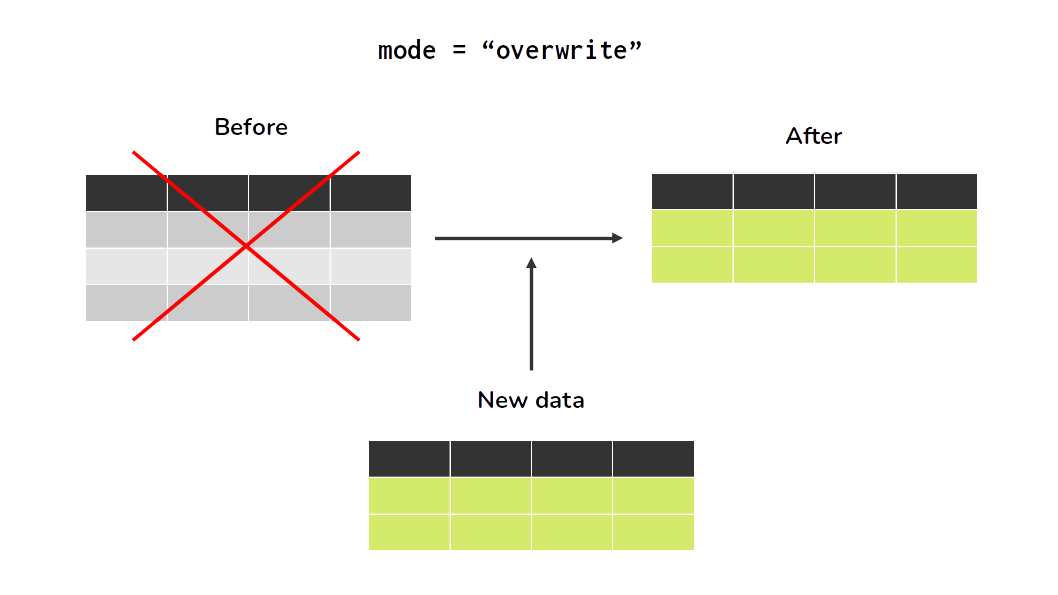
\includegraphics{Chapters/./../Figures/table-save-modes-overwrite.png}

}

}

\subcaption{\label{fig-mode-overwrite}Mode overwrite}
\end{minipage}%
\newline
\begin{minipage}[t]{\linewidth}

{\centering 

\raisebox{-\height}{

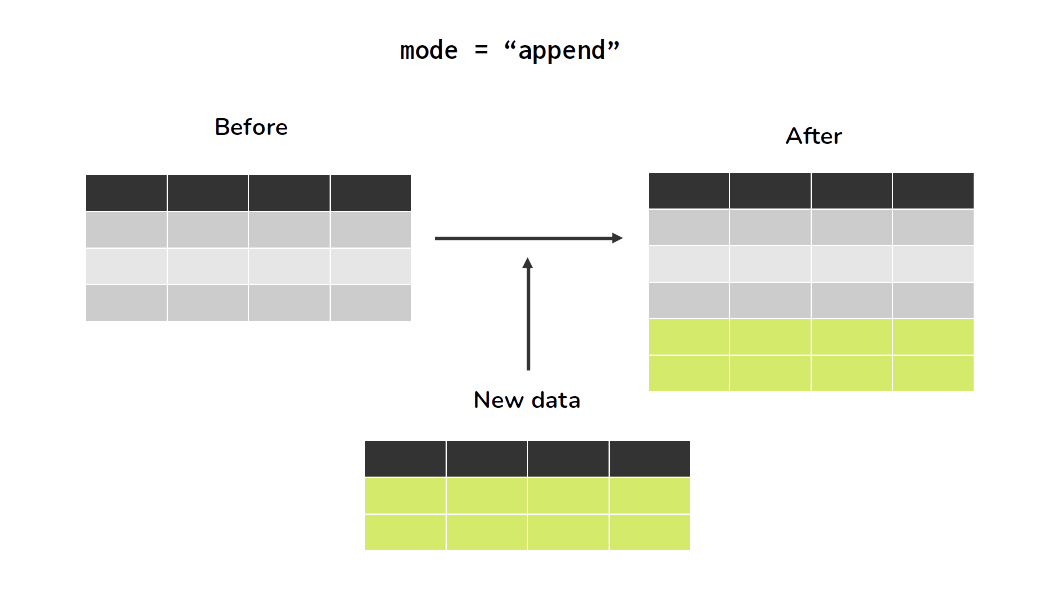
\includegraphics{Chapters/./../Figures/table-save-modes-append.png}

}

}

\subcaption{\label{fig-mode-append}Mode append}
\end{minipage}%

\caption{\label{fig-save-table-modes}How Spark saves your data with
different ``save modes''}

\end{figure}

You can see the full list of arguments of \texttt{write.SaveAsTable()},
and their description by
\href{https://spark.apache.org/docs/3.1.2/api/python/reference/api/pyspark.sql.DataFrameWriter.saveAsTable}{looking
at the documentation}\footnote{\url{https://spark.apache.org/docs/3.1.2/api/python/reference/api/pyspark.sql.DataFrameWriter.saveAsTable}}.

\hypertarget{sec-temp-persist}{%
\subsection{Temporary versus Persistent
sources}\label{sec-temp-persist}}

When you register any Spark DataFrame as a SQL \texttt{TABLE}, it
becomes a persistent source. Because the contents, the data, the rows of
the table are stored on disk, inside a database, and can be accessed any
time, even after you close or restart your computer (or your Spark
Session). In other words, it becomes ``persistent'' as in the sense of
``it does not die''.

As another example, when you save a specific SQL query as a SQL
\texttt{VIEW} with the \texttt{CREATE\ VIEW} statement, this SQL
\texttt{VIEW} is saved inside the database. As a consequence, it becomes
a persistent source as well, and can be accessed and reused in other
Spark Sessions, unless you explicit drop (or ``remove'') this SQL
\texttt{VIEW} with a \texttt{DROP\ VIEW} statement.

However, with methods like \texttt{createTempView()} and
\texttt{createOrReplaceTempView()} you register your Spark DataFrame as
a \emph{temporary} SQL \texttt{VIEW}. This means that the life (or time
of existence) of this \texttt{VIEW} is tied to your Spark Session. In
other words, it will exist in your Spark SQL Catalog only for the
duration of your Spark Session. When you close your Spark Session, this
\texttt{VIEW} just dies. When you start a new Spark Session it does not
exist anymore. As a result, you have to register your DataFrame again at
the catalog to use it one more time.

\hypertarget{spark-sql-catalog-is-the-bridge-between-sql-and-pyspark}{%
\subsection{\texorpdfstring{Spark SQL Catalog is the bridge between SQL
and
\texttt{pyspark}}{Spark SQL Catalog is the bridge between SQL and pyspark}}\label{spark-sql-catalog-is-the-bridge-between-sql-and-pyspark}}

Remember, to run SQL queries over any Spark DataFrame, you must register
this DataFrame into the Spark SQL Catalog. Because of it, this Spark SQL
Catalog works almost as the bridge that connects the python objects that
hold your Spark DataFrames to the Spark SQL context. Without it, Spark
SQL will not find your Spark DataFrames. As a result, it can not run any
SQL query over it.

When you try to use a DataFrame that is not currently registered at the
Spark SQL Catalog, Spark will automatically raise a
\texttt{AnalysisException}, like in the example below:

\begin{Shaded}
\begin{Highlighting}[]
\NormalTok{spark}\OperatorTok{\textbackslash{}}
\NormalTok{  .sql(}\StringTok{"SELECT * FROM this.does\_not\_exist"}\NormalTok{)}\OperatorTok{\textbackslash{}}
\NormalTok{  .show()}
\end{Highlighting}
\end{Shaded}

\begin{verbatim}
AnalysisException: Table or view not found
\end{verbatim}

The methods \texttt{saveAsTable()}, \texttt{createTempView()} and
\texttt{createOrReplaceTempView()} are the main methods to register your
Spark DataFrame into this Spark SQL Catalog. This means that you have to
use one of these methods before you run any SQL query over your Spark
DataFrame.

\hypertarget{the-penguins-dataframe}{%
\section{\texorpdfstring{The \texttt{penguins}
DataFrame}{The penguins DataFrame}}\label{the-penguins-dataframe}}

Over the next examples in this chapter, we will explore the
\texttt{penguins} DataFrame. This is the \texttt{penguins} dataset from
the
\href{https://allisonhorst.github.io/palmerpenguins/}{\texttt{palmerpenguins}
R library}. It stores data of multiple measurements of penguin species
from the islands in Palmer Archipelago.

These measurements include size (flipper length, body mass, bill
dimensions) and sex, and they were collected by researchers of the
Antarctica LTER program, a member of the Long Term Ecological Research
Network. If you want to understand more about each field/column present
in this dataset, I recommend you to read the
\href{https://allisonhorst.github.io/palmerpenguins/reference/penguins.html}{official
documentation of this dataset}\footnote{\url{https://allisonhorst.github.io/palmerpenguins/reference/penguins.html}}.

To get this data, you can download the CSV file called
\texttt{penguins.csv} (remember that this CSV can be downloaded from the
book repository\footnote{\url{https://github.com/pedropark99/Introd-pyspark/tree/main/Data}}).
In the code below, I am reading this CSV file and creating a Spark
DataFrame with its data. Then, I register this Spark DataFrame as a SQL
temporary view (called \texttt{penguins\_view}) using the
\texttt{createOrReplaceTempView()} method.

\begin{Shaded}
\begin{Highlighting}[]
\NormalTok{path }\OperatorTok{=} \StringTok{"../Data/penguins.csv"}
\NormalTok{penguins }\OperatorTok{=}\NormalTok{ spark.read}\OperatorTok{\textbackslash{}}
\NormalTok{  .csv(path, header }\OperatorTok{=} \VariableTok{True}\NormalTok{)}
  
\NormalTok{penguins.createOrReplaceTempView(}\StringTok{\textquotesingle{}penguins\_view\textquotesingle{}}\NormalTok{)}
\end{Highlighting}
\end{Shaded}

After these commands, I have now a SQL view called
\texttt{penguins\_view} registered in my Spark SQL context, which I can
query it, using pure SQL:

\begin{Shaded}
\begin{Highlighting}[]
\NormalTok{spark.sql(}\StringTok{\textquotesingle{}SELECT * FROM penguins\_view\textquotesingle{}}\NormalTok{).show(}\DecValTok{5}\NormalTok{)}
\end{Highlighting}
\end{Shaded}

\begin{verbatim}
+-------+---------+--------------+-------------+-----------------+-----------+------+----+
|species|   island|bill_length_mm|bill_depth_mm|flipper_length_mm|body_mass_g|   sex|year|
+-------+---------+--------------+-------------+-----------------+-----------+------+----+
| Adelie|Torgersen|          39.1|         18.7|              181|       3750|  male|2007|
| Adelie|Torgersen|          39.5|         17.4|              186|       3800|female|2007|
| Adelie|Torgersen|          40.3|           18|              195|       3250|female|2007|
| Adelie|Torgersen|          null|         null|             null|       null|  null|2007|
| Adelie|Torgersen|          36.7|         19.3|              193|       3450|female|2007|
+-------+---------+--------------+-------------+-----------------+-----------+------+----+
only showing top 5 rows
\end{verbatim}

\hypertarget{selecting-your-spark-dataframes}{%
\section{Selecting your Spark
DataFrames}\label{selecting-your-spark-dataframes}}

An obvious way to access any SQL \texttt{TABLE} or \texttt{VIEW}
registered in your Spark SQL context, is to select it, through a simple
\texttt{SELECT\ *\ FROM} statement, like we saw in the previous
examples. However, it can be quite annoying to type ``SELECT * FROM''
every time you want to use a SQL \texttt{TABLE} or \texttt{VIEW} in
Spark SQL.

That is why Spark offers a shortcut to us, which is the \texttt{table()}
method of your Spark session. In other words, the code
\texttt{spark.table("table\_name")} is a shortcut to
\texttt{spark.sql("SELECT\ *\ FROM\ table\_name")}. They both mean the
same thing. For example, we could access \texttt{penguins\_view} as:

\begin{Shaded}
\begin{Highlighting}[]
\NormalTok{spark}\OperatorTok{\textbackslash{}}
\NormalTok{  .table(}\StringTok{\textquotesingle{}penguins\_view\textquotesingle{}}\NormalTok{)}\OperatorTok{\textbackslash{}}
\NormalTok{  .show(}\DecValTok{5}\NormalTok{)}
\end{Highlighting}
\end{Shaded}

\begin{verbatim}
+-------+---------+--------------+-------------+-----------------+-----------+------+----+
|species|   island|bill_length_mm|bill_depth_mm|flipper_length_mm|body_mass_g|   sex|year|
+-------+---------+--------------+-------------+-----------------+-----------+------+----+
| Adelie|Torgersen|          39.1|         18.7|              181|       3750|  male|2007|
| Adelie|Torgersen|          39.5|         17.4|              186|       3800|female|2007|
| Adelie|Torgersen|          40.3|           18|              195|       3250|female|2007|
| Adelie|Torgersen|          null|         null|             null|       null|  null|2007|
| Adelie|Torgersen|          36.7|         19.3|              193|       3450|female|2007|
+-------+---------+--------------+-------------+-----------------+-----------+------+----+
only showing top 5 rows
\end{verbatim}

\hypertarget{executing-sql-expressions}{%
\section{Executing SQL expressions}\label{executing-sql-expressions}}

As I noted at Section~\ref{sec-columns-related-expressions}, columns of
a Spark DataFrame (or objects of class \texttt{Column}) are closely
related to expressions. As a result, you usually use and execute
expressions in Spark when you want to transform (or mutate) columns of a
Spark DataFrame.

This is no different for SQL expressions. A SQL expression is basically
any expression you would use on the \texttt{SELECT} statement of your
SQL query. As you can probably guess, since they are used in the
\texttt{SELECT} statement, these expressions are used to transform
columns of a Spark DataFrame.

There are many column transformations that are particularly verbose and
expensive to write in ``pure'' \texttt{pyspark}. But you can use a SQL
expression in your favor, to translate this transformation into a more
short and concise form. Virtually any expression you write in
\texttt{pyspark} can be translated into a SQL expression.

To execute a SQL expression, you give this expression inside a string to
the \texttt{expr()} function from the \texttt{pyspark.sql.functions}
module. Since expressions are used to transform columns, you normally
use the \texttt{expr()} function inside a \texttt{withColumn()} or a
\texttt{select()} DataFrame method, like in the example below:

\begin{Shaded}
\begin{Highlighting}[]
\ImportTok{from}\NormalTok{ pyspark.sql.functions }\ImportTok{import}\NormalTok{ expr}

\NormalTok{spark}\OperatorTok{\textbackslash{}}
\NormalTok{  .table(}\StringTok{\textquotesingle{}penguins\_view\textquotesingle{}}\NormalTok{)}\OperatorTok{\textbackslash{}}
\NormalTok{  .withColumn(}
    \StringTok{\textquotesingle{}specie\_island\textquotesingle{}}\NormalTok{,}
\NormalTok{    expr(}\StringTok{"CONCAT(species, \textquotesingle{}\_\textquotesingle{}, island)"}\NormalTok{)}
\NormalTok{  )}\OperatorTok{\textbackslash{}}
\NormalTok{  .withColumn(}
    \StringTok{\textquotesingle{}sex\_short\textquotesingle{}}\NormalTok{,}
\NormalTok{    expr(}\StringTok{"CASE WHEN sex == \textquotesingle{}male\textquotesingle{} THEN \textquotesingle{}M\textquotesingle{} ELSE \textquotesingle{}F\textquotesingle{} END"}\NormalTok{)}
\NormalTok{  )}\OperatorTok{\textbackslash{}}
\NormalTok{  .select(}\StringTok{\textquotesingle{}specie\_island\textquotesingle{}}\NormalTok{, }\StringTok{\textquotesingle{}sex\_short\textquotesingle{}}\NormalTok{)}\OperatorTok{\textbackslash{}}
\NormalTok{  .show(}\DecValTok{5}\NormalTok{)}
\end{Highlighting}
\end{Shaded}

\begin{verbatim}
+----------------+---------+
|   specie_island|sex_short|
+----------------+---------+
|Adelie_Torgersen|        M|
|Adelie_Torgersen|        F|
|Adelie_Torgersen|        F|
|Adelie_Torgersen|        F|
|Adelie_Torgersen|        F|
+----------------+---------+
only showing top 5 rows
\end{verbatim}

I particulaly like to write ``if-else'' or ``case-when'' statements
using a pure \texttt{CASE\ WHEN} SQL statement inside the
\texttt{expr()} function. By using this strategy you usually get a more
simple statement that translates the intention of your code in a cleaner
way. But if I wrote the exact same \texttt{CASE\ WHEN} statement above
using pure \texttt{pyspark} functions, I would end up with a shorter
(but ``less clean'') statement using the \texttt{when()} and
\texttt{otherwise()} functions:

\begin{Shaded}
\begin{Highlighting}[]
\ImportTok{from}\NormalTok{ pyspark.sql.functions }\ImportTok{import}\NormalTok{ (}
\NormalTok{  when, col,}
\NormalTok{  concat, lit}
\NormalTok{)}

\NormalTok{spark}\OperatorTok{\textbackslash{}}
\NormalTok{  .table(}\StringTok{\textquotesingle{}penguins\_view\textquotesingle{}}\NormalTok{)}\OperatorTok{\textbackslash{}}
\NormalTok{  .withColumn(}
    \StringTok{\textquotesingle{}specie\_island\textquotesingle{}}\NormalTok{,}
\NormalTok{    concat(}\StringTok{\textquotesingle{}species\textquotesingle{}}\NormalTok{, lit(}\StringTok{\textquotesingle{}\_\textquotesingle{}}\NormalTok{), }\StringTok{\textquotesingle{}island\textquotesingle{}}\NormalTok{)}
\NormalTok{  )}\OperatorTok{\textbackslash{}}
\NormalTok{  .withColumn(}
    \StringTok{\textquotesingle{}sex\_short\textquotesingle{}}\NormalTok{,}
\NormalTok{    when(col(}\StringTok{"sex"}\NormalTok{) }\OperatorTok{==} \StringTok{\textquotesingle{}male\textquotesingle{}}\NormalTok{, }\StringTok{\textquotesingle{}M\textquotesingle{}}\NormalTok{)}\OperatorTok{\textbackslash{}}
\NormalTok{      .otherwise(}\StringTok{\textquotesingle{}F\textquotesingle{}}\NormalTok{)}
\NormalTok{  )}\OperatorTok{\textbackslash{}}
\NormalTok{  .select(}\StringTok{\textquotesingle{}specie\_island\textquotesingle{}}\NormalTok{, }\StringTok{\textquotesingle{}sex\_short\textquotesingle{}}\NormalTok{)}\OperatorTok{\textbackslash{}}
\NormalTok{  .show(}\DecValTok{5}\NormalTok{)}
\end{Highlighting}
\end{Shaded}

\begin{verbatim}
+----------------+---------+
|   specie_island|sex_short|
+----------------+---------+
|Adelie_Torgersen|        M|
|Adelie_Torgersen|        F|
|Adelie_Torgersen|        F|
|Adelie_Torgersen|        F|
|Adelie_Torgersen|        F|
+----------------+---------+
only showing top 5 rows
\end{verbatim}

\hypertarget{every-dataframe-transformation-in-python-can-be-translated-into-sql}{%
\section{Every DataFrame transformation in Python can be translated into
SQL}\label{every-dataframe-transformation-in-python-can-be-translated-into-sql}}

All DataFrame API transformations that you write in Python (using
\texttt{pyspark}) can be translated into SQL queries/expressions using
the Spark SQL module. Since the DataFrame API is a core part of
\texttt{pyspark}, the majority of python code you write with
\texttt{pyspark} can be translated into SQL queries (if you wanto to).

Is worth pointing out, that, no matter which language you choose (Python
or SQL), they are both further compiled to the same base instructions.
The end result is that the Python code you write and his SQL translated
version \textbf{will perform the same} (they have the same efficiency),
because they are compiled to the same instructions before being executed
by Spark.

\hypertarget{dataframe-methods-are-usually-translated-into-sql-keywords}{%
\subsection{DataFrame methods are usually translated into SQL
keywords}\label{dataframe-methods-are-usually-translated-into-sql-keywords}}

When you translate the methods from the python \texttt{DataFrame} class
(like \texttt{orderBy()}, \texttt{select()} and \texttt{where()}) into
their equivalents in Spark SQL, you usually get SQL keywords (like
\texttt{ORDER\ BY}, \texttt{SELECT} and \texttt{WHERE}).

For example, if I needed to get the top 5 penguins with the biggest body
mass at \texttt{penguins\_view}, that had sex equal to
\texttt{"female"}, and, ordered by bill length, I could run the
following python code:

\begin{Shaded}
\begin{Highlighting}[]
\ImportTok{from}\NormalTok{ pyspark.sql.functions }\ImportTok{import}\NormalTok{ col}
\NormalTok{top\_5 }\OperatorTok{=}\NormalTok{ penguins}\OperatorTok{\textbackslash{}}
\NormalTok{    .where(col(}\StringTok{\textquotesingle{}sex\textquotesingle{}}\NormalTok{) }\OperatorTok{==} \StringTok{\textquotesingle{}female\textquotesingle{}}\NormalTok{)}\OperatorTok{\textbackslash{}}
\NormalTok{    .orderBy(col(}\StringTok{\textquotesingle{}body\_mass\_g\textquotesingle{}}\NormalTok{).desc())}\OperatorTok{\textbackslash{}}
\NormalTok{    .limit(}\DecValTok{5}\NormalTok{)}

\NormalTok{top\_5}\OperatorTok{\textbackslash{}}
\NormalTok{    .orderBy(}\StringTok{\textquotesingle{}bill\_length\_mm\textquotesingle{}}\NormalTok{)}\OperatorTok{\textbackslash{}}
\NormalTok{    .show()}
\end{Highlighting}
\end{Shaded}

\begin{verbatim}
+-------+------+--------------+-------------+-----------------+-----------+------+----+
|species|island|bill_length_mm|bill_depth_mm|flipper_length_mm|body_mass_g|   sex|year|
+-------+------+--------------+-------------+-----------------+-----------+------+----+
| Gentoo|Biscoe|          44.9|         13.3|              213|       5100|female|2008|
| Gentoo|Biscoe|          45.1|         14.5|              207|       5050|female|2007|
| Gentoo|Biscoe|          45.2|         14.8|              212|       5200|female|2009|
| Gentoo|Biscoe|          46.5|         14.8|              217|       5200|female|2008|
| Gentoo|Biscoe|          49.1|         14.8|              220|       5150|female|2008|
+-------+------+--------------+-------------+-----------------+-----------+------+----+
\end{verbatim}

I could translate the above python code to the following SQL query:

\begin{Shaded}
\begin{Highlighting}[]
\KeywordTok{WITH}\NormalTok{ top\_5 }\KeywordTok{AS}\NormalTok{ (}
    \KeywordTok{SELECT} \OperatorTok{*}
    \KeywordTok{FROM}\NormalTok{ penguins\_view}
    \KeywordTok{WHERE}\NormalTok{ sex }\OperatorTok{==} \StringTok{\textquotesingle{}female\textquotesingle{}}
    \KeywordTok{ORDER} \KeywordTok{BY}\NormalTok{ body\_mass\_g }\KeywordTok{DESC}
    \KeywordTok{LIMIT} \DecValTok{5}
\NormalTok{)}

\KeywordTok{SELECT} \OperatorTok{*}
\KeywordTok{FROM}\NormalTok{ top\_5}
\KeywordTok{ORDER} \KeywordTok{BY}\NormalTok{ bill\_length\_mm}
\end{Highlighting}
\end{Shaded}

Again, to execute the above SQL query inside \texttt{pyspark} we need to
give this query as a string to the \texttt{sql()} method of our Spark
Session, like this:

\begin{Shaded}
\begin{Highlighting}[]
\NormalTok{query }\OperatorTok{=} \StringTok{\textquotesingle{}\textquotesingle{}\textquotesingle{}}
\StringTok{WITH top\_5 AS (}
\StringTok{    SELECT *}
\StringTok{    FROM penguins\_view}
\StringTok{    WHERE sex == \textquotesingle{}female\textquotesingle{}}
\StringTok{    ORDER BY body\_mass\_g DESC}
\StringTok{    LIMIT 5}
\StringTok{)}

\StringTok{SELECT *}
\StringTok{FROM top\_5}
\StringTok{ORDER BY bill\_length\_mm}
\StringTok{\textquotesingle{}\textquotesingle{}\textquotesingle{}}

\CommentTok{\# The same result of the example above}
\NormalTok{spark.sql(query)}
\end{Highlighting}
\end{Shaded}

\begin{verbatim}
DataFrame[species: string, island: string, bill_length_mm: string, bill_depth_mm: string, flipper_length_mm: string, body_mass_g: string, sex: string, year: string]
\end{verbatim}

\hypertarget{spark-functions-are-usually-translated-into-sql-functions}{%
\subsection{Spark functions are usually translated into SQL
functions}\label{spark-functions-are-usually-translated-into-sql-functions}}

Every function from the \texttt{pyspark.sql.functions} module you might
use to describe your transformations in python, can be directly used in
Spark SQL. In other words, every Spark function that is accesible in
python, is also accesible in Spark SQL.

When you translate these python functions into SQL, they usually become
a pure SQL function with the same name. For example, if I wanted to use
the \texttt{regexp\_extract()} python function, from the
\texttt{pyspark.sql.functions} module in Spark SQL, I just use the
\texttt{REGEXP\_EXTRACT()} SQL function. The same occurs to any other
function, like the \texttt{to\_date()} function for example.

\begin{Shaded}
\begin{Highlighting}[]
\ImportTok{from}\NormalTok{ pyspark.sql.functions }\ImportTok{import}\NormalTok{ to\_date, regexp\_extract}
\CommentTok{\# \textasciigrave{}df1\textasciigrave{} and \textasciigrave{}df2\textasciigrave{} are both equal. Because they both}
\CommentTok{\# use the same \textasciigrave{}to\_date()\textasciigrave{} and \textasciigrave{}regexp\_extract()\textasciigrave{} functions}
\NormalTok{df1 }\OperatorTok{=}\NormalTok{ (spark}
\NormalTok{  .table(}\StringTok{\textquotesingle{}penguins\_view\textquotesingle{}}\NormalTok{)}
\NormalTok{  .withColumn(}
    \StringTok{\textquotesingle{}extract\_number\textquotesingle{}}\NormalTok{,}
\NormalTok{    regexp\_extract(}\StringTok{\textquotesingle{}bill\_length\_mm\textquotesingle{}}\NormalTok{, }\StringTok{\textquotesingle{}[0{-}9]+\textquotesingle{}}\NormalTok{, }\DecValTok{0}\NormalTok{)}
\NormalTok{  )}
\NormalTok{  .withColumn(}\StringTok{\textquotesingle{}date\textquotesingle{}}\NormalTok{, to\_date(}\StringTok{\textquotesingle{}year\textquotesingle{}}\NormalTok{, }\StringTok{\textquotesingle{}y\textquotesingle{}}\NormalTok{))}
\NormalTok{  .select(}
    \StringTok{\textquotesingle{}bill\_length\_mm\textquotesingle{}}\NormalTok{, }\StringTok{\textquotesingle{}year\textquotesingle{}}\NormalTok{,}
    \StringTok{\textquotesingle{}extract\_number\textquotesingle{}}\NormalTok{, }\StringTok{\textquotesingle{}date\textquotesingle{}}
\NormalTok{  )}
\NormalTok{)}

\NormalTok{df2 }\OperatorTok{=}\NormalTok{ (spark}
\NormalTok{  .table(}\StringTok{\textquotesingle{}penguins\_view\textquotesingle{}}\NormalTok{)}
\NormalTok{  .withColumn(}
    \StringTok{\textquotesingle{}extract\_number\textquotesingle{}}\NormalTok{,}
\NormalTok{    expr(}\StringTok{"REGEXP\_EXTRACT(bill\_length\_mm, \textquotesingle{}[0{-}9]+\textquotesingle{}, 0)"}\NormalTok{)}
\NormalTok{  )}
\NormalTok{  .withColumn(}\StringTok{\textquotesingle{}date\textquotesingle{}}\NormalTok{, expr(}\StringTok{"TO\_DATE(year, \textquotesingle{}y\textquotesingle{})"}\NormalTok{))}
\NormalTok{  .select(}
    \StringTok{\textquotesingle{}bill\_length\_mm\textquotesingle{}}\NormalTok{, }\StringTok{\textquotesingle{}year\textquotesingle{}}\NormalTok{,}
    \StringTok{\textquotesingle{}extract\_number\textquotesingle{}}\NormalTok{, }\StringTok{\textquotesingle{}date\textquotesingle{}}
\NormalTok{  )}
\NormalTok{)}

\NormalTok{df2.show(}\DecValTok{5}\NormalTok{)}
\end{Highlighting}
\end{Shaded}

\begin{verbatim}
+--------------+----+--------------+----------+
|bill_length_mm|year|extract_number|      date|
+--------------+----+--------------+----------+
|          39.1|2007|            39|2007-01-01|
|          39.5|2007|            39|2007-01-01|
|          40.3|2007|            40|2007-01-01|
|          null|2007|          null|2007-01-01|
|          36.7|2007|            36|2007-01-01|
+--------------+----+--------------+----------+
only showing top 5 rows
\end{verbatim}

This is very handy. Because for every new python function from the
\texttt{pyspark.sql.functions} module, that you learn how to use, you
automatically learn how to use in Spark SQL as well, because is the same
function, with the basically the same name and arguments.

As an example, I could easily translate the above transformations that
use the \texttt{to\_date()} and \texttt{regexp\_extract()} python
functions, into the following SQL query (that I could easily execute
trough the \texttt{sql()} Spark Session method):

\begin{Shaded}
\begin{Highlighting}[]
\KeywordTok{SELECT} 
\NormalTok{  bill\_length\_mm, }\DataTypeTok{year}\NormalTok{,}
\NormalTok{  REGEXP\_EXTRACT(bill\_length\_mm, }\StringTok{\textquotesingle{}[0{-}9]+\textquotesingle{}}\NormalTok{, }\DecValTok{0}\NormalTok{) }\KeywordTok{AS}\NormalTok{ extract\_number,}
  \FunctionTok{TO\_DATE}\NormalTok{(}\DataTypeTok{year}\NormalTok{, }\StringTok{\textquotesingle{}y\textquotesingle{}}\NormalTok{) }\KeywordTok{AS} \DataTypeTok{date}
\KeywordTok{FROM}\NormalTok{ penguins\_view}
\end{Highlighting}
\end{Shaded}

\bookmarksetup{startatroot}

\hypertarget{sec-string-tools}{%
\chapter{Tools for string manipulation}\label{sec-string-tools}}

Many of the world's data is represented (or stored) as text (or string
variables). As a consequence, is very important to know the tools
available to process and transform this kind of data, in any platform
you use. In this chapter, we will focus on these tools.

Most of the functionality available in \texttt{pyspark} to process text
data comes from functions available at the
\texttt{pyspark.sql.functions} module. This means that processing and
transforming text data in Spark usually involves applying a function on
a column of a Spark DataFrame (by using DataFrame methods such as
\texttt{withColumn()} and \texttt{select()}).

\hypertarget{the-logs-dataframe}{%
\section{\texorpdfstring{The \texttt{logs}
DataFrame}{The logs DataFrame}}\label{the-logs-dataframe}}

Over the next examples in this chapter, we will use the \texttt{logs}
DataFrame, which contains various log messages registered at a
fictitious IP adress. The data that represents this DataFrame is freely
available trough the \texttt{logs.json} file, which you can download
from the official repository of this book\footnote{\url{https://github.com/pedropark99/Introd-pyspark/tree/main/Data}}.

Each line of this JSON file contains a message that was recorded by the
logger of a fictitious system. Each log message have three main parts,
which are: 1) the type of message (warning - \texttt{WARN}, information
- \texttt{INFO}, error - \texttt{ERROR}); 2) timestamp of the event; 3)
the content of the message. In the example below, we have an example of
message:

\begin{quote}
{[}INFO{]}: 2022-09-05 03:35:01.43 Looking for workers at South America
region;
\end{quote}

To import \texttt{logs.json} file into a Spark DataFrame, I can use the
following code:

\begin{Shaded}
\begin{Highlighting}[]
\NormalTok{path }\OperatorTok{=} \StringTok{\textquotesingle{}./../Data/logs.json\textquotesingle{}}
\NormalTok{logs }\OperatorTok{=}\NormalTok{ spark.read.json(path)}
\NormalTok{n\_truncate }\OperatorTok{=} \DecValTok{50}
\NormalTok{logs.show(}\DecValTok{5}\NormalTok{, truncate }\OperatorTok{=}\NormalTok{ n\_truncate)}
\end{Highlighting}
\end{Shaded}

\begin{verbatim}
+--------------+--------------------------------------------------+
|            ip|                                           message|
+--------------+--------------------------------------------------+
|  1.0.104.27  |[INFO]: 2022-09-05 03:35:01.43 Looking for work...|
|  1.0.104.27  |[WARN]: 2022-09-05 03:35:58.007 Workers are una...|
|  1.0.104.27  |[INFO]: 2022-09-05 03:40:59.054 Looking for wor...|
|  1.0.104.27  |[INFO]: 2022-09-05 03:42:24 3 Workers were acqu...|
|  1.0.104.27  |[INFO]: 2022-09-05 03:42:37 Initializing instan...|
+--------------+--------------------------------------------------+
only showing top 5 rows
\end{verbatim}

By default, when we use the \texttt{show()} action to see the contents
of our Spark DataFrame, Spark will always truncate (or cut) any value in
the DataFrame that is more than 20 characters long. Since the logs
messages in the \texttt{logs.json} file are usually much longer than 20
characters, I am using the \texttt{truncate} argument of \texttt{show()}
in the example above, to avoid this behaviour.

By setting this argument to 50, I am asking Spark to truncate (or cut)
values at the 50th character (instead of the 20th). By doing this, you
(reader) can actually see a much more significant part of the logs
messages in the result above.

\hypertarget{changing-the-case-of-letters-in-a-string}{%
\section{Changing the case of letters in a
string}\label{changing-the-case-of-letters-in-a-string}}

Probably the most basic string transformation that exists is to change
the case of the letters (or characters) that compose the string. That
is, to raise specific letters to upper-case, or reduce them to
lower-case, and vice-versa.

As a first example, lets go back to the \texttt{logs} DataFrame, and try
to change all messages in this DataFrame to lower case, upper case and
title case, by using the \texttt{lower()}, \texttt{upper()}, and
\texttt{initcap()} functions from the \texttt{pyspark.sql.functions}
module.

\begin{Shaded}
\begin{Highlighting}[]
\ImportTok{from}\NormalTok{ pyspark.sql.functions }\ImportTok{import}\NormalTok{ (}
\NormalTok{    lower,}
\NormalTok{    upper,}
\NormalTok{    initcap}
\NormalTok{)}

\NormalTok{m }\OperatorTok{=}\NormalTok{ logs.select(}\StringTok{\textquotesingle{}message\textquotesingle{}}\NormalTok{)}
\CommentTok{\# Change to lower case:}
\NormalTok{m.withColumn(}\StringTok{\textquotesingle{}message\textquotesingle{}}\NormalTok{, lower(}\StringTok{\textquotesingle{}message\textquotesingle{}}\NormalTok{))}\OperatorTok{\textbackslash{}}
\NormalTok{    .show(}\DecValTok{5}\NormalTok{, truncate }\OperatorTok{=}\NormalTok{ n\_truncate)}
\end{Highlighting}
\end{Shaded}

\begin{verbatim}
+--------------------------------------------------+
|                                           message|
+--------------------------------------------------+
|[info]: 2022-09-05 03:35:01.43 looking for work...|
|[warn]: 2022-09-05 03:35:58.007 workers are una...|
|[info]: 2022-09-05 03:40:59.054 looking for wor...|
|[info]: 2022-09-05 03:42:24 3 workers were acqu...|
|[info]: 2022-09-05 03:42:37 initializing instan...|
+--------------------------------------------------+
only showing top 5 rows
\end{verbatim}

\begin{Shaded}
\begin{Highlighting}[]
\CommentTok{\# Change to upper case:}
\NormalTok{m.withColumn(}\StringTok{\textquotesingle{}message\textquotesingle{}}\NormalTok{, upper(}\StringTok{\textquotesingle{}message\textquotesingle{}}\NormalTok{))}\OperatorTok{\textbackslash{}}
\NormalTok{    .show(}\DecValTok{5}\NormalTok{, truncate }\OperatorTok{=}\NormalTok{ n\_truncate)}
\end{Highlighting}
\end{Shaded}

\begin{verbatim}
+--------------------------------------------------+
|                                           message|
+--------------------------------------------------+
|[INFO]: 2022-09-05 03:35:01.43 LOOKING FOR WORK...|
|[WARN]: 2022-09-05 03:35:58.007 WORKERS ARE UNA...|
|[INFO]: 2022-09-05 03:40:59.054 LOOKING FOR WOR...|
|[INFO]: 2022-09-05 03:42:24 3 WORKERS WERE ACQU...|
|[INFO]: 2022-09-05 03:42:37 INITIALIZING INSTAN...|
+--------------------------------------------------+
only showing top 5 rows
\end{verbatim}

\begin{Shaded}
\begin{Highlighting}[]
\CommentTok{\# Change to title case}
\CommentTok{\# (first letter of each word is upper case):}
\NormalTok{m.withColumn(}\StringTok{\textquotesingle{}message\textquotesingle{}}\NormalTok{, initcap(}\StringTok{\textquotesingle{}message\textquotesingle{}}\NormalTok{))}\OperatorTok{\textbackslash{}}
\NormalTok{    .show(}\DecValTok{5}\NormalTok{, truncate }\OperatorTok{=}\NormalTok{ n\_truncate)}
\end{Highlighting}
\end{Shaded}

\begin{verbatim}
+--------------------------------------------------+
|                                           message|
+--------------------------------------------------+
|[info]: 2022-09-05 03:35:01.43 Looking For Work...|
|[warn]: 2022-09-05 03:35:58.007 Workers Are Una...|
|[info]: 2022-09-05 03:40:59.054 Looking For Wor...|
|[info]: 2022-09-05 03:42:24 3 Workers Were Acqu...|
|[info]: 2022-09-05 03:42:37 Initializing Instan...|
+--------------------------------------------------+
only showing top 5 rows
\end{verbatim}

\hypertarget{calculating-string-length}{%
\section{Calculating string length}\label{calculating-string-length}}

In Spark, you can use the \texttt{length()} function to get the length
(i.e.~the number of characters) of a string. In the example below, we
can see that the first log message is 74 characters long, while the
second log message have 112 characters.

\begin{Shaded}
\begin{Highlighting}[]
\ImportTok{from}\NormalTok{ pyspark.sql.functions }\ImportTok{import}\NormalTok{ length}
\NormalTok{logs}\OperatorTok{\textbackslash{}}
\NormalTok{    .withColumn(}\StringTok{\textquotesingle{}length\textquotesingle{}}\NormalTok{, length(}\StringTok{\textquotesingle{}message\textquotesingle{}}\NormalTok{))}\OperatorTok{\textbackslash{}}
\NormalTok{    .show(}\DecValTok{5}\NormalTok{)}
\end{Highlighting}
\end{Shaded}

\begin{verbatim}
+--------------+--------------------+------+
|            ip|             message|length|
+--------------+--------------------+------+
|  1.0.104.27  |[INFO]: 2022-09-0...|    74|
|  1.0.104.27  |[WARN]: 2022-09-0...|   112|
|  1.0.104.27  |[INFO]: 2022-09-0...|    75|
|  1.0.104.27  |[INFO]: 2022-09-0...|    94|
|  1.0.104.27  |[INFO]: 2022-09-0...|    65|
+--------------+--------------------+------+
only showing top 5 rows
\end{verbatim}

\hypertarget{trimming-or-removing-spaces-from-strings}{%
\section{Trimming or removing spaces from
strings}\label{trimming-or-removing-spaces-from-strings}}

The process of removing unnecessary spaces from strings is usually
called ``trimming''. In Spark, we have three functions that do this
process, which are:

\begin{itemize}
\tightlist
\item
  \texttt{trim()}: removes spaces from both sides of the string;
\item
  \texttt{ltrim()}: removes spaces from the left side of the string;
\item
  \texttt{rtrim()}: removes spaces from the right side of the string;
\end{itemize}

\begin{Shaded}
\begin{Highlighting}[]
\ImportTok{from}\NormalTok{ pyspark.sql.functions }\ImportTok{import}\NormalTok{ (}
\NormalTok{    trim, rtrim, ltrim}
\NormalTok{)}

\NormalTok{logs}\OperatorTok{\textbackslash{}}
\NormalTok{    .select(}\StringTok{\textquotesingle{}ip\textquotesingle{}}\NormalTok{)}\OperatorTok{\textbackslash{}}
\NormalTok{    .withColumn(}\StringTok{\textquotesingle{}ip\_trim\textquotesingle{}}\NormalTok{, trim(}\StringTok{\textquotesingle{}ip\textquotesingle{}}\NormalTok{))}\OperatorTok{\textbackslash{}}
\NormalTok{    .withColumn(}\StringTok{\textquotesingle{}ip\_ltrim\textquotesingle{}}\NormalTok{, ltrim(}\StringTok{\textquotesingle{}ip\textquotesingle{}}\NormalTok{))}\OperatorTok{\textbackslash{}}
\NormalTok{    .withColumn(}\StringTok{\textquotesingle{}ip\_rtrim\textquotesingle{}}\NormalTok{, rtrim(}\StringTok{\textquotesingle{}ip\textquotesingle{}}\NormalTok{))}\OperatorTok{\textbackslash{}}
\NormalTok{    .show(}\DecValTok{5}\NormalTok{)}
\end{Highlighting}
\end{Shaded}

\begin{verbatim}
+--------------+----------+------------+------------+
|            ip|   ip_trim|    ip_ltrim|    ip_rtrim|
+--------------+----------+------------+------------+
|  1.0.104.27  |1.0.104.27|1.0.104.27  |  1.0.104.27|
|  1.0.104.27  |1.0.104.27|1.0.104.27  |  1.0.104.27|
|  1.0.104.27  |1.0.104.27|1.0.104.27  |  1.0.104.27|
|  1.0.104.27  |1.0.104.27|1.0.104.27  |  1.0.104.27|
|  1.0.104.27  |1.0.104.27|1.0.104.27  |  1.0.104.27|
+--------------+----------+------------+------------+
only showing top 5 rows
\end{verbatim}

For the most part, I tend to remove these unnecessary strings when I
want to: 1) tidy the values; 2) avoid weird and confusing mistakes in
filters on my DataFrame. The second case is worth describing in more
details.

Let's suppose you wanted to filter all rows from the \texttt{logs}
DataFrame where \texttt{ip} is equal to the \texttt{1.0.104.27} IP
adress. However, you can see in the result above, that I get nothing.
Not a single row of result.

\begin{Shaded}
\begin{Highlighting}[]
\ImportTok{from}\NormalTok{ pyspark.sql.functions }\ImportTok{import}\NormalTok{ col}
\NormalTok{logs.}\BuiltInTok{filter}\NormalTok{(col(}\StringTok{\textquotesingle{}ip\textquotesingle{}}\NormalTok{) }\OperatorTok{==} \StringTok{"1.0.104.27"}\NormalTok{)}\OperatorTok{\textbackslash{}}
\NormalTok{    .show(}\DecValTok{5}\NormalTok{)}
\end{Highlighting}
\end{Shaded}

\begin{verbatim}
+---+-------+
| ip|message|
+---+-------+
+---+-------+
\end{verbatim}

But if you see the result of the previous example (where we appliead the
three versions of ``trim functions''), you know that this IP adress
\texttt{1.0.104.27} exists in the DataFrame. You know that the filter
above should find values for this IP adress. So why it did not find any
rows?

The answer is these annoying (and hidden) spaces on both sides of the
values from the \texttt{ip} column. If we remove these unnecessary
spaces from the values of the \texttt{ip} column, we suddenly find the
rows that we were looking for.

\begin{Shaded}
\begin{Highlighting}[]
\NormalTok{logs.}\BuiltInTok{filter}\NormalTok{(trim(col(}\StringTok{\textquotesingle{}ip\textquotesingle{}}\NormalTok{)) }\OperatorTok{==} \StringTok{"1.0.104.27"}\NormalTok{)}\OperatorTok{\textbackslash{}}
\NormalTok{    .show(}\DecValTok{5}\NormalTok{)}
\end{Highlighting}
\end{Shaded}

\begin{verbatim}
+--------------+--------------------+
|            ip|             message|
+--------------+--------------------+
|  1.0.104.27  |[INFO]: 2022-09-0...|
|  1.0.104.27  |[WARN]: 2022-09-0...|
|  1.0.104.27  |[INFO]: 2022-09-0...|
|  1.0.104.27  |[INFO]: 2022-09-0...|
|  1.0.104.27  |[INFO]: 2022-09-0...|
+--------------+--------------------+
only showing top 5 rows
\end{verbatim}

\hypertarget{extracting-substrings}{%
\section{Extracting substrings}\label{extracting-substrings}}

There are five main functions that we can use in order to extract
substrings of a string, which are:

\begin{itemize}
\tightlist
\item
  \texttt{substring()} and \texttt{substr()}: extract a single substring
  based on a start position and the length (number of characters) of the
  collected substring\footnote{These functions uses a one based index,
    and not zero based index.};
\item
  \texttt{substring\_index()}: extract a single substring based on a
  single delimiter\footnote{These functions uses a one based index, and
    not zero based index.};
\item
  \texttt{split()}: extract one or multiple substrings based on commom
  delimiter;
\item
  \texttt{regexp\_extract()}: extracts substrings from a given string
  that match a specified regular expression pattern;
\end{itemize}

You can obviously extract a substring that matches a particular regex
(regular expression) by using the \texttt{regexp\_extract()} function.
However, I will describe this function, and the regex functionality
available in \texttt{pyspark} at Section~\ref{sec-regex}, or, more
specifically, at Section~\ref{sec-regexp-extract}. For now, just
understand that you can also use regex to extract substrings from your
text data.

\hypertarget{a-substring-based-on-a-start-position-and-length}{%
\subsection{A substring based on a start position and
length}\label{a-substring-based-on-a-start-position-and-length}}

The \texttt{substring()} and \texttt{substr()} functions they both work
the same way. However, they come from different places. The
\texttt{substring()} function comes from the
\texttt{spark.sql.functions} module, while the \texttt{substr()}
function is actually a method from the \texttt{Column} class.

One interesting aspect of these functions, is that they both use a
one-based index, instead of a zero-based index. This means that the
first character in the full string is identified by the index 1, instead
of the index 0.

The first argument in both function is the index that identifies the
start of the substring. If you set this argument to, let's say, 4, it
means that the substring you want to extract starts at the 4th character
in the input string.

The second argument is the amount of characters in the substring, or, in
other words, it's length. For example, if you set this argument to 10,
it means that the function will extract the substring that is formed by
walking \(10 - 1 = 9\) characters ahead from the start position you
specified at the first argument. We can also interpret this as: the
function will walk ahead on the string, from the start position, until
it gets a substring that is 10 characters long.

In the example below, we are extracting the substring that starts at the
second character (index 2) and ends at the sixth character (index 6) in
the string.

\begin{Shaded}
\begin{Highlighting}[]
\ImportTok{from}\NormalTok{ pyspark.sql.functions }\ImportTok{import}\NormalTok{ col, substring}
\CommentTok{\# \textasciigrave{}df1\textasciigrave{} and \textasciigrave{}df2\textasciigrave{} are equal, because}
\CommentTok{\# they both mean the same thing}
\NormalTok{df1 }\OperatorTok{=}\NormalTok{ (logs}
\NormalTok{    .withColumn(}\StringTok{\textquotesingle{}sub\textquotesingle{}}\NormalTok{, col(}\StringTok{\textquotesingle{}message\textquotesingle{}}\NormalTok{).substr(}\DecValTok{2}\NormalTok{, }\DecValTok{5}\NormalTok{))}
\NormalTok{)}

\NormalTok{df2 }\OperatorTok{=}\NormalTok{ (logs}
\NormalTok{    .withColumn(}\StringTok{\textquotesingle{}sub\textquotesingle{}}\NormalTok{, substring(}\StringTok{\textquotesingle{}message\textquotesingle{}}\NormalTok{, }\DecValTok{2}\NormalTok{, }\DecValTok{5}\NormalTok{))}
\NormalTok{)}

\NormalTok{df2.show(}\DecValTok{5}\NormalTok{)}
\end{Highlighting}
\end{Shaded}

\begin{verbatim}
+--------------+--------------------+-----+
|            ip|             message|  sub|
+--------------+--------------------+-----+
|  1.0.104.27  |[INFO]: 2022-09-0...|INFO]|
|  1.0.104.27  |[WARN]: 2022-09-0...|WARN]|
|  1.0.104.27  |[INFO]: 2022-09-0...|INFO]|
|  1.0.104.27  |[INFO]: 2022-09-0...|INFO]|
|  1.0.104.27  |[INFO]: 2022-09-0...|INFO]|
+--------------+--------------------+-----+
only showing top 5 rows
\end{verbatim}

Just to be very clear on how \texttt{substring()} and \texttt{substr()}
both works. The Figure~\ref{fig-substring-start-length} illustrates the
result of the above code.

\begin{figure}

{\centering 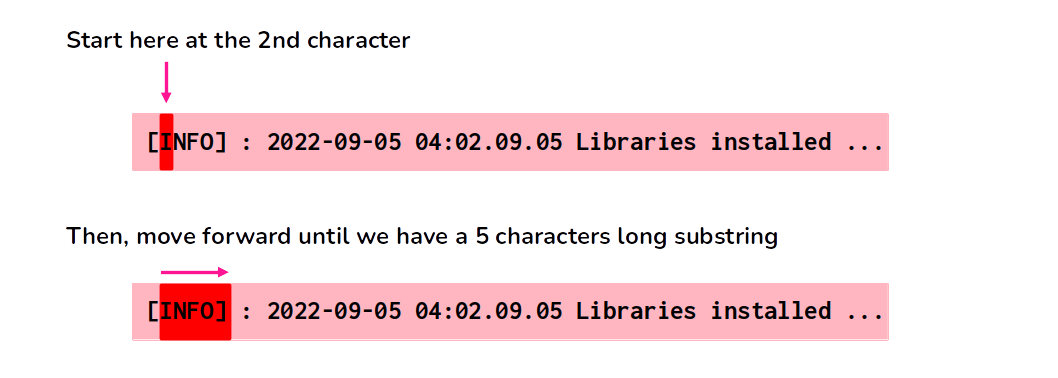
\includegraphics{Chapters/./../Figures/substring-start-length.png}

}

\caption{\label{fig-substring-start-length}How \texttt{substring()} and
\texttt{substr()} works}

\end{figure}

\hypertarget{a-substring-based-on-a-delimiter}{%
\subsection{A substring based on a
delimiter}\label{a-substring-based-on-a-delimiter}}

The \texttt{substring\_index()} function works very differently. It
collects the substring formed between the start of the string, and the
nth occurrence of a particular character.

For example, if you ask \texttt{substring\_index()} to search for the
3rd occurrence of the character \texttt{\$} in your string, the function
will return to you the substring formed by all characters that are
between the start of the string until the 3rd occurrence of this
character \texttt{\$}. You can also ask \texttt{substring\_index()} to
read backwards. That is, to start the search on the end of the string,
and move backwards in the string until it gets to the 3rd occurrence of
this character \texttt{\$}.

As an example, let's look at the 10th log message present in the
\texttt{logs} DataFrame. I used the \texttt{collect()} DataFrame method
to collect this message into a raw python string, so we can see the full
message.

\begin{Shaded}
\begin{Highlighting}[]
\ImportTok{from}\NormalTok{ pyspark.sql.functions }\ImportTok{import}\NormalTok{ monotonically\_increasing\_id}

\NormalTok{mes\_10th }\OperatorTok{=}\NormalTok{ (}
\NormalTok{    logs}
\NormalTok{    .withColumn(}
        \StringTok{\textquotesingle{}row\_id\textquotesingle{}}\NormalTok{,}
\NormalTok{        monotonically\_increasing\_id()}
\NormalTok{    )}
\NormalTok{    .where(col(}\StringTok{\textquotesingle{}row\_id\textquotesingle{}}\NormalTok{) }\OperatorTok{==} \DecValTok{9}\NormalTok{)}
\NormalTok{)}

\NormalTok{message }\OperatorTok{=}\NormalTok{ mes\_10th.collect()[}\DecValTok{0}\NormalTok{][}\StringTok{\textquotesingle{}message\textquotesingle{}}\NormalTok{]}
\BuiltInTok{print}\NormalTok{(message)}
\end{Highlighting}
\end{Shaded}

\begin{verbatim}
[INFO]: 2022-09-05 04:02:09.05 Libraries installed: pandas, flask, numpy, spark_map, pyspark
\end{verbatim}

We can see that this log message is listing a set of libraries that were
installed somewhere. Suppose you want to collect the first and the last
libraries in this list. How would you do it?

A good start to this objective, is to isolate the list of libraries from
the rest of the message. In other words, there is a bunch of characters
in the start of the log message, that we do not care about. So let's get
rid of them.

If you look closely to the message, you can see that the character
\texttt{:} appears twice whithin the message. One close to the start of
the string, and another time right before the start of the list of the
libraries. We can use this character as our first delimiter, to collect
the third substring that it creates within the total string, which is
the substring that contains the list of libraries.

This first stage is presented visually at
Figure~\ref{fig-substring-delimiter1}.

\begin{figure}

{\centering 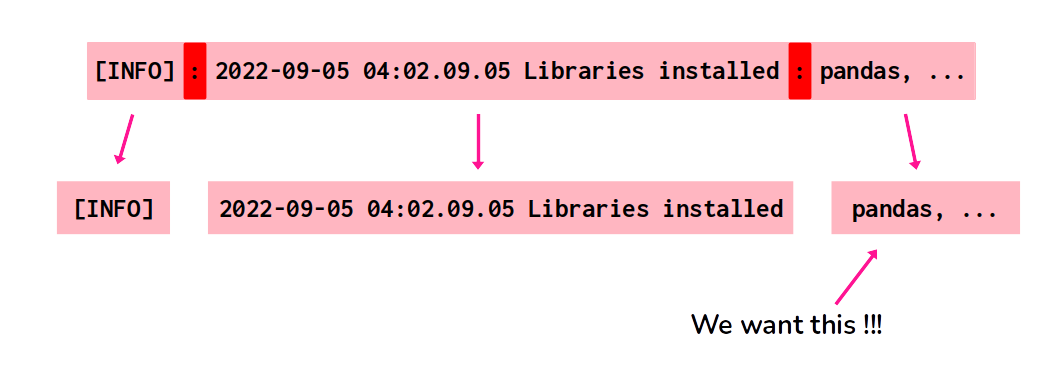
\includegraphics{Chapters/./../Figures/substring-delimiter1.png}

}

\caption{\label{fig-substring-delimiter1}The first stage of subsetting}

\end{figure}

Now that we identified the substrings produced by the ``delimiter
character'', we just need to understand better which index we need to
use in \texttt{substring\_index()} to get this third substring that we
want. The Figure~\ref{fig-substring-delimiter2} presents in a visual
manner how the count system of \texttt{substring\_index()} works.

When you use a positive index, \texttt{substring\_index()} will count
the occurrences of the delimiter character from left to right. But, when
you use a negative index, the opposite happens. That is,
\texttt{substring\_index()} counts the occurrences of the delimiter
character from right to left.

\begin{figure}

{\centering 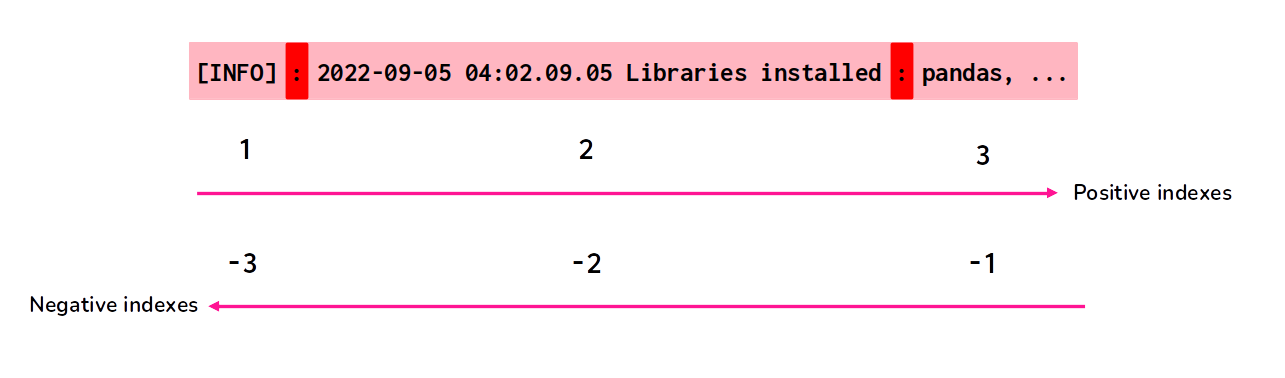
\includegraphics{Chapters/./../Figures/substring-delimiter2.png}

}

\caption{\label{fig-substring-delimiter2}The count system of
\texttt{substring\_index()}}

\end{figure}

The index 1 represents the first substring that is before the the 1st
occurence of the delimiter (\texttt{{[}INFO{]}}). The index 2 represents
everything that is before the 2nd occurence of the delimiter
(\texttt{{[}INFO{]}:\ 2022-09-05\ 04:02.09.05\ Libraries\ installed}).
etc.

In contrast, the index -1 represents everything that is after the 1st
occurence of the delimiter, couting from right to left
(\texttt{pandas,\ flask,\ numpy,\ spark\_map,\ pyspark}). The index -2
represents everything that is after the 2nd occurence of the delimiter
(\texttt{2022-09-05\ 04:02.09.05\ Libraries\ installed:\ pandas,\ flask,\ numpy,\ spark\_map,\ pyspark}).
Again, couting from right to left.

Having all these informations in mind, we can conclude that the
following code fit our first objective. Note that I applied the
\texttt{trim()} function over the result of \texttt{substring\_index()},
to ensure that the result substring does not contain any unnecessary
spaces at both ends.

\begin{Shaded}
\begin{Highlighting}[]
\ImportTok{from}\NormalTok{ pyspark.sql.functions }\ImportTok{import}\NormalTok{ substring\_index}
\NormalTok{mes\_10th }\OperatorTok{=}\NormalTok{ mes\_10th}\OperatorTok{\textbackslash{}}
\NormalTok{    .withColumn(}
        \StringTok{\textquotesingle{}list\_of\_libraries\textquotesingle{}}\NormalTok{,}
\NormalTok{        trim(substring\_index(}\StringTok{\textquotesingle{}message\textquotesingle{}}\NormalTok{, }\StringTok{\textquotesingle{}:\textquotesingle{}}\NormalTok{, }\OperatorTok{{-}}\DecValTok{1}\NormalTok{))}
\NormalTok{    )}

\NormalTok{mes\_10th.select(}\StringTok{\textquotesingle{}list\_of\_libraries\textquotesingle{}}\NormalTok{)}\OperatorTok{\textbackslash{}}
\NormalTok{    .show(truncate }\OperatorTok{=}\NormalTok{ n\_truncate)}
\end{Highlighting}
\end{Shaded}

\begin{verbatim}
+----------------------------------------+
|                       list_of_libraries|
+----------------------------------------+
|pandas, flask, numpy, spark_map, pyspark|
+----------------------------------------+
\end{verbatim}

\hypertarget{forming-an-array-of-substrings}{%
\subsection{Forming an array of
substrings}\label{forming-an-array-of-substrings}}

Now is a good time to introduce the \texttt{split()} function, because
we can use it to extract the first and the last library from the list
libraries of stored at the \texttt{mes\_10th} DataFrame. Basically, this
function also uses a delimiter character to cut the total string into
multiple pieces, and store these pieces in a array of substrings. With
this strategy, we can now access each substring (or each piece of the
total string) individually.

If we look again at the string that we stored at the
\texttt{list\_of\_libraries} column, we have a list of libraries,
separated by a comma.

\begin{Shaded}
\begin{Highlighting}[]
\NormalTok{mes\_10th}\OperatorTok{\textbackslash{}}
\NormalTok{    .select(}\StringTok{\textquotesingle{}list\_of\_libraries\textquotesingle{}}\NormalTok{)}\OperatorTok{\textbackslash{}}
\NormalTok{    .show(truncate }\OperatorTok{=}\NormalTok{ n\_truncate)}
\end{Highlighting}
\end{Shaded}

\begin{verbatim}
+----------------------------------------+
|                       list_of_libraries|
+----------------------------------------+
|pandas, flask, numpy, spark_map, pyspark|
+----------------------------------------+
\end{verbatim}

The comma character (\texttt{,}) plays an important role in this string,
by separating each value in the list. And we can use this comma
character as the delimiter inside \texttt{split()}, to get an array of
substrings. Each element of this array is one of the many libraries in
the list. The Figure~\ref{fig-string-split} presents this process
visually.

\begin{figure}

{\centering 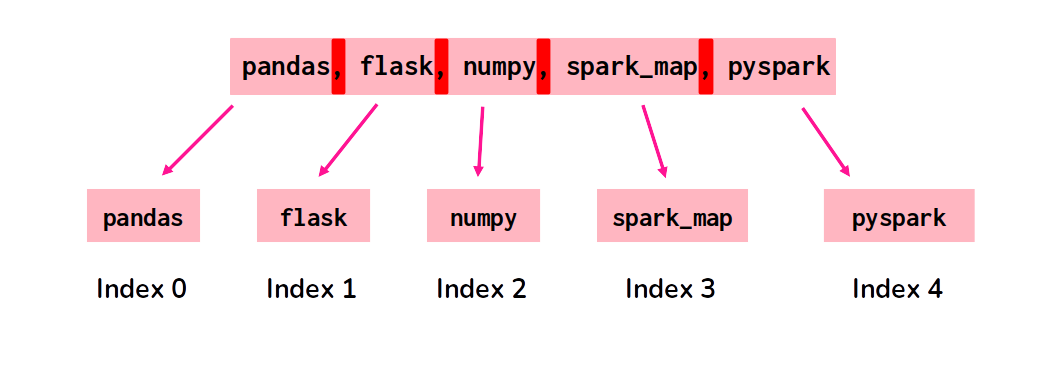
\includegraphics{Chapters/./../Figures/string-split.png}

}

\caption{\label{fig-string-split}Building an array of substrings with
\texttt{split()}}

\end{figure}

The code to make this process is very straightforward. In the example
below, the column \texttt{array\_of\_libraries} becomes a column of data
type \texttt{ArrayType(StringType)}, that is, an array of string values.

\begin{Shaded}
\begin{Highlighting}[]
\ImportTok{from}\NormalTok{ pyspark.sql.functions }\ImportTok{import}\NormalTok{ split}
\NormalTok{mes\_10th }\OperatorTok{=}\NormalTok{ mes\_10th}\OperatorTok{\textbackslash{}}
\NormalTok{    .withColumn(}
        \StringTok{\textquotesingle{}array\_of\_libraries\textquotesingle{}}\NormalTok{,}
\NormalTok{        split(}\StringTok{\textquotesingle{}list\_of\_libraries\textquotesingle{}}\NormalTok{, }\StringTok{\textquotesingle{}, \textquotesingle{}}\NormalTok{)}
\NormalTok{    )}

\NormalTok{mes\_10th}\OperatorTok{\textbackslash{}}
\NormalTok{    .select(}\StringTok{\textquotesingle{}array\_of\_libraries\textquotesingle{}}\NormalTok{)}\OperatorTok{\textbackslash{}}
\NormalTok{    .show(truncate }\OperatorTok{=}\NormalTok{ n\_truncate)}
\end{Highlighting}
\end{Shaded}

\begin{verbatim}
+------------------------------------------+
|                        array_of_libraries|
+------------------------------------------+
|[pandas, flask, numpy, spark_map, pyspark]|
+------------------------------------------+
\end{verbatim}

By having this array of substring, we can very easily select a specific
element in this array, by using the \texttt{getItem()} column method,
or, by using the open brackets as you would normally use to select an
element in a python list.

You just need to give the index of the element you want to select, like
in the example below that we select the first and the fifth libraries in
the array.

\begin{Shaded}
\begin{Highlighting}[]
\NormalTok{mes\_10th}\OperatorTok{\textbackslash{}}
\NormalTok{    .withColumn(}\StringTok{\textquotesingle{}lib\_1\textquotesingle{}}\NormalTok{, col(}\StringTok{\textquotesingle{}array\_of\_libraries\textquotesingle{}}\NormalTok{)[}\DecValTok{0}\NormalTok{])}\OperatorTok{\textbackslash{}}
\NormalTok{    .withColumn(}\StringTok{\textquotesingle{}lib\_5\textquotesingle{}}\NormalTok{, col(}\StringTok{\textquotesingle{}array\_of\_libraries\textquotesingle{}}\NormalTok{).getItem(}\DecValTok{4}\NormalTok{))}\OperatorTok{\textbackslash{}}
\NormalTok{    .select(}\StringTok{\textquotesingle{}lib\_1\textquotesingle{}}\NormalTok{, }\StringTok{\textquotesingle{}lib\_5\textquotesingle{}}\NormalTok{)}\OperatorTok{\textbackslash{}}
\NormalTok{    .show(truncate }\OperatorTok{=}\NormalTok{ n\_truncate)}
\end{Highlighting}
\end{Shaded}

\begin{verbatim}
+------+-------+
| lib_1|  lib_5|
+------+-------+
|pandas|pyspark|
+------+-------+
\end{verbatim}

\hypertarget{concatenating-multiple-strings-together}{%
\section{Concatenating multiple strings
together}\label{concatenating-multiple-strings-together}}

Sometimes, we need to concatenate multiple strings together, to form a
single and longer string. To do this process, Spark offers two main
functions, which are: \texttt{concat()} and \texttt{concat\_ws()}. Both
of these functions receives a list of columns as input, and will perform
the same task, which is to concatenate the values of each column in the
list, sequentially.

However, the \texttt{concat\_ws()} function have an extra argument
called \texttt{sep}, where you can define a string to be used as the
separator (or the ``delimiter'') between the values of each column in
the list. In some way, this \texttt{sep} argument and the
\texttt{concat\_ws()} function works very similarly to the
\href{https://docs.python.org/3/library/stdtypes.html\#str.join}{\texttt{join()}
string method of python}\footnote{\url{https://docs.python.org/3/library/stdtypes.html\#str.join}}.

Let's comeback to the \texttt{penguins} DataFrame to demonstrate the use
of these functions:

\begin{Shaded}
\begin{Highlighting}[]
\NormalTok{path }\OperatorTok{=} \StringTok{"../Data/penguins.csv"}
\NormalTok{penguins }\OperatorTok{=}\NormalTok{ spark.read}\OperatorTok{\textbackslash{}}
\NormalTok{    .csv(path, header }\OperatorTok{=} \VariableTok{True}\NormalTok{)}

\NormalTok{penguins.select(}\StringTok{\textquotesingle{}species\textquotesingle{}}\NormalTok{, }\StringTok{\textquotesingle{}island\textquotesingle{}}\NormalTok{, }\StringTok{\textquotesingle{}sex\textquotesingle{}}\NormalTok{)}\OperatorTok{\textbackslash{}}
\NormalTok{    .show(}\DecValTok{5}\NormalTok{)}
\end{Highlighting}
\end{Shaded}

\begin{verbatim}
+-------+---------+------+
|species|   island|   sex|
+-------+---------+------+
| Adelie|Torgersen|  male|
| Adelie|Torgersen|female|
| Adelie|Torgersen|female|
| Adelie|Torgersen|  null|
| Adelie|Torgersen|female|
+-------+---------+------+
only showing top 5 rows
\end{verbatim}

Suppose you wanted to concatenate the values of the columns
\texttt{species}, \texttt{island} and \texttt{sex} together, and, store
these new values on a separate column. All you need to do is to list
these columns inside the \texttt{concat()} or \texttt{concat\_ws()}
function.

If you look at the example below, you can see that I also used the
\texttt{lit()} function to add a underline character (\texttt{\_})
between the values of each column. This is more verbose, because if you
needed to concatenate 10 columns together, and still add a ``delimiter
character'' (like the underline) between the values of each column, you
would have to write \texttt{lit(\textquotesingle{}\_\textquotesingle{})}
for 9 times on the list.

In contrast, the \texttt{concat\_ws()} offers a much more succinct way
of expressing this same operation. Because the first argument of
\texttt{concat\_ws()} is the character to be used as the delimiter
between each column, and, after that, we have the list of columns to be
concatenated.

\begin{Shaded}
\begin{Highlighting}[]
\ImportTok{from}\NormalTok{ pyspark.sql.functions }\ImportTok{import}\NormalTok{ (}
\NormalTok{    concat,}
\NormalTok{    concat\_ws,}
\NormalTok{    lit}
\NormalTok{)}

\NormalTok{penguins}\OperatorTok{\textbackslash{}}
\NormalTok{    .withColumn(}
        \StringTok{\textquotesingle{}using\_concat\textquotesingle{}}\NormalTok{,}
\NormalTok{        concat(}
            \StringTok{\textquotesingle{}species\textquotesingle{}}\NormalTok{, lit(}\StringTok{\textquotesingle{}\_\textquotesingle{}}\NormalTok{), }\StringTok{\textquotesingle{}island\textquotesingle{}}\NormalTok{,}
\NormalTok{            lit(}\StringTok{\textquotesingle{}\_\textquotesingle{}}\NormalTok{), }\StringTok{\textquotesingle{}sex\textquotesingle{}}\NormalTok{)}
\NormalTok{    )}\OperatorTok{\textbackslash{}}
\NormalTok{    .withColumn(}
        \StringTok{\textquotesingle{}using\_concat\_ws\textquotesingle{}}\NormalTok{,}
\NormalTok{        concat\_ws(}
            \StringTok{\textquotesingle{}\_\textquotesingle{}}\NormalTok{, }\CommentTok{\# The delimiter character}
            \StringTok{\textquotesingle{}species\textquotesingle{}}\NormalTok{, }\StringTok{\textquotesingle{}island\textquotesingle{}}\NormalTok{, }\StringTok{\textquotesingle{}sex\textquotesingle{}} \CommentTok{\# The list of columns}
\NormalTok{        )}
\NormalTok{    )}\OperatorTok{\textbackslash{}}
\NormalTok{    .select(}\StringTok{\textquotesingle{}using\_concat\textquotesingle{}}\NormalTok{, }\StringTok{\textquotesingle{}using\_concat\_ws\textquotesingle{}}\NormalTok{)}\OperatorTok{\textbackslash{}}
\NormalTok{    .show(}\DecValTok{5}\NormalTok{, truncate }\OperatorTok{=}\NormalTok{ n\_truncate)}
\end{Highlighting}
\end{Shaded}

\begin{verbatim}
+-----------------------+-----------------------+
|           using_concat|        using_concat_ws|
+-----------------------+-----------------------+
|  Adelie_Torgersen_male|  Adelie_Torgersen_male|
|Adelie_Torgersen_female|Adelie_Torgersen_female|
|Adelie_Torgersen_female|Adelie_Torgersen_female|
|                   null|       Adelie_Torgersen|
|Adelie_Torgersen_female|Adelie_Torgersen_female|
+-----------------------+-----------------------+
only showing top 5 rows
\end{verbatim}

If you look closely to the result above, you can also see, that
\texttt{concat()} and \texttt{concat\_ws()} functions deal with null
values in different ways. If \texttt{concat()} finds a null value for a
particular row, in any of the listed columns to be concatenated, the end
result of the process is a null value for that particular row.

On the other hand, \texttt{concat\_ws()} will try to concatenate as many
values as he can. If he does find a null value, he just ignores this
null value and go on to the next column, until it hits the last column
in the list.

\hypertarget{sec-regex}{%
\section{Introducing regular expressions}\label{sec-regex}}

Spark also provides some basic regex (\emph{regular expressions})
functionality. Most of this functionality is available trough two
functions that comes from the \texttt{pyspark.sql.functions} module,
which are:

\begin{itemize}
\tightlist
\item
  \texttt{regexp\_replace()}: replaces all occurrences of a specified
  regular expression pattern in a given string with a replacement
  string.;
\item
  \texttt{regexp\_extract()}: extracts substrings from a given string
  that match a specified regular expression pattern;
\end{itemize}

There is also a column method that provides an useful way of testing if
the values of a column matchs a regular expression or not, which is the
\texttt{rlike()} column method. You can use the \texttt{rlike()} method
in conjunction with the \texttt{filter()} or \texttt{where()} DataFrame
methods, to find all values that fit (or match) a particular regular
expression, like we demonstrated at
Section~\ref{sec-filter-regex-pattern}.

\hypertarget{the-java-regular-expression-standard}{%
\subsection{The Java regular expression
standard}\label{the-java-regular-expression-standard}}

At this point, is worth remembering a basic fact about Apache Spark that
we introduced at Chapter~\ref{sec-introd-spark}. Apache Spark is written
in Scala, which is a modern programming language deeply connected with
the Java programming language. One of the many consequences from this
fact, is that all regular expression functionality available in Apache
Spark is based on the Java \texttt{java.util.regex} package.

This means that you should always write regular expressions on your
\texttt{pyspark} code that follows the Java regular expression syntax,
and not the Python regular expression syntax, which is based on the
python module \texttt{re}.

Although this detail is important, these two flavors of regular
expressions (Python syntax versus Java syntax) are very, very similar.
So, for the most part, you should not see any difference between these
two syntaxes.

If for some reason, you need to consult the full list of all
metacharacters available in the Java regular expression standard, you
can always check the Java documentation for the \texttt{java.util.regex}
package. More specifically, the
\href{https://docs.oracle.com/javase/8/docs/api/java/util/regex/Pattern.html}{documentation
for the \texttt{java.util.regex.Pattern} class}\footnote{\url{https://docs.oracle.com/javase/8/docs/api/java/util/regex/Pattern.html}}.

The following list gives you a quick description of a small fraction of
the available metacharacters in the Java syntax, and, as a result,
metacharacters that you can use in \texttt{pyspark}:

\begin{itemize}
\tightlist
\item
  \texttt{.} : Matches any single character;
\item
  \texttt{*} : Matches zero or more occurrences of the preceding
  character or pattern;
\item
  \texttt{+} : Matches one or more occurrences of the preceding
  character or pattern;
\item
  \texttt{?} : Matches zero or one occurrence of the preceding character
  or pattern;
\item
  \texttt{\textbar{}} : Matches either the expression before or after
  the \texttt{\textbar{}};
\item
  \texttt{{[}{]}} : Matches any single character within the brackets;
\item
  \texttt{\textbackslash{}d} : Matches any digit character;
\item
  \texttt{\textbackslash{}b} : Matches a word boundary character;
\item
  \texttt{\textbackslash{}w} : Matches any word character. Equivalente
  to the
  \texttt{"\textbackslash{}b({[}a-zA-Z\_0-9{]}+)\textbackslash{}b"}
  regular expression;
\item
  \texttt{\textbackslash{}s} : Matches any whitespace character;
\item
  \texttt{()} : Groups a series of pattern elements to a single element;
\end{itemize}

\hypertarget{using-an-invalid-regular-expression}{%
\subsection{Using an invalid regular
expression}\label{using-an-invalid-regular-expression}}

When you write an invalid regular expression in your code, Spark usually
complains with a \texttt{java.util.regex.PatternSyntaxException} runtime
error. The code presented below is an example of code that produces such
error.

In this example, the regular expression
\texttt{\textbackslash{}b({[}a-z{]}} is invalid because it is missing a
closing parenthesis. If you try to execute this code, Spark will raise a
with the message ``Unclosed group near index 7''. This error message
indicates that there is a syntax error in the regular expression, due to
an unclosed group (i.e., a missing closing parenthesis).

\begin{Shaded}
\begin{Highlighting}[]
\ImportTok{from}\NormalTok{ pyspark.sql.functions }\ImportTok{import}\NormalTok{ col}
\NormalTok{weird\_regex }\OperatorTok{=} \StringTok{\textquotesingle{}}\CharTok{\textbackslash{}b}\StringTok{([a{-}z]\textquotesingle{}}
\NormalTok{logs}\OperatorTok{\textbackslash{}}
\NormalTok{    .}\BuiltInTok{filter}\NormalTok{(col(}\StringTok{\textquotesingle{}message\textquotesingle{}}\NormalTok{).rlike(weird\_regex))}\OperatorTok{\textbackslash{}}
\NormalTok{    .show(}\DecValTok{5}\NormalTok{)}
\end{Highlighting}
\end{Shaded}

\begin{verbatim}
Py4JJavaError: An error occurred while calling o261.showString.
:   java.util.regex.PatternSyntaxException: Unclosed group near index 7
([a-z]
\end{verbatim}

To avoid these runtime errors, due to invalid regular expressions, is
always a good idea to test your regular expressions, before you use them
in your \texttt{pyspark} code. You can easily test your regular
expressions by using online tools, such as the
\href{https://regex101.com/}{Regex101 website}\footnote{\url{https://regex101.com/}}.

\hypertarget{sec-regexp-replace}{%
\subsection{\texorpdfstring{Replacing occurrences of a particular
regular expression with
\texttt{regexp\_replace()}}{Replacing occurrences of a particular regular expression with regexp\_replace()}}\label{sec-regexp-replace}}

One of the most essential actions with regular expression is to find
text that fits into a particular regular expression, and, rewriting this
text into a different format, or, even removing it completely from the
string.

The \texttt{regexp\_replace()} function (from the
\texttt{pyspark.sql.functions} module) is the function that allows you
to perform this kind of operation on string values of a column in a
Spark DataFrame.

This function replaces all occurrences of a specified regular expression
pattern in a given string with a replacement string, and it takes three
different arguments:

\begin{itemize}
\tightlist
\item
  The input column name or expression that contains the string values to
  be modified;
\item
  The regular expression pattern to search for within the input string
  values;
\item
  The replacement string that will replace all occurrences of the
  matched pattern in the input string values;
\end{itemize}

As an example, lets suppose we want to remove completely the type of the
message in all log messages present in the \texttt{logs} DataFrame. To
that, we first need to get a regular expression capable of identifying
all possibilities for these types.

A potential candidate would be the regular expression
\texttt{\textquotesingle{}\textbackslash{}\textbackslash{}{[}(INFO\textbar{}ERROR\textbar{}WARN)\textbackslash{}\textbackslash{}{]}:\ \textquotesingle{}},
so lets give it a shot. Since we are trying to \textbf{remove} this
particular part from all log messages, we should replace this part of
the string by an empty string
(\texttt{\textquotesingle{}\textquotesingle{}}), like in the example
below:

\begin{Shaded}
\begin{Highlighting}[]
\ImportTok{from}\NormalTok{ pyspark.sql.functions }\ImportTok{import}\NormalTok{ regexp\_replace}

\NormalTok{type\_regex }\OperatorTok{=} \StringTok{\textquotesingle{}}\CharTok{\textbackslash{}\textbackslash{}}\StringTok{[(INFO|ERROR|WARN)}\CharTok{\textbackslash{}\textbackslash{}}\StringTok{]: \textquotesingle{}}

\NormalTok{logs}\OperatorTok{\textbackslash{}}
\NormalTok{    .withColumn(}
        \StringTok{\textquotesingle{}without\_type\textquotesingle{}}\NormalTok{,}
\NormalTok{        regexp\_replace(}\StringTok{\textquotesingle{}message\textquotesingle{}}\NormalTok{, type\_regex, }\StringTok{\textquotesingle{}\textquotesingle{}}\NormalTok{)}
\NormalTok{    )}\OperatorTok{\textbackslash{}}
\NormalTok{    .select(}\StringTok{\textquotesingle{}message\textquotesingle{}}\NormalTok{, }\StringTok{\textquotesingle{}without\_type\textquotesingle{}}\NormalTok{)}\OperatorTok{\textbackslash{}}
\NormalTok{    .show(truncate }\OperatorTok{=} \DecValTok{30}\NormalTok{)}
\end{Highlighting}
\end{Shaded}

\begin{verbatim}
+------------------------------+------------------------------+
|                       message|                  without_type|
+------------------------------+------------------------------+
|[INFO]: 2022-09-05 03:35:01...|2022-09-05 03:35:01.43 Look...|
|[WARN]: 2022-09-05 03:35:58...|2022-09-05 03:35:58.007 Wor...|
|[INFO]: 2022-09-05 03:40:59...|2022-09-05 03:40:59.054 Loo...|
|[INFO]: 2022-09-05 03:42:24...|2022-09-05 03:42:24 3 Worke...|
|[INFO]: 2022-09-05 03:42:37...|2022-09-05 03:42:37 Initial...|
|[WARN]: 2022-09-05 03:52:02...|2022-09-05 03:52:02.98 Libr...|
|[INFO]: 2022-09-05 04:00:33...|2022-09-05 04:00:33.210 Lib...|
|[INFO]: 2022-09-05 04:01:15...|2022-09-05 04:01:15 All clu...|
|[INFO]: 2022-09-05 04:01:35...|2022-09-05 04:01:35.022 Mak...|
|[INFO]: 2022-09-05 04:02:09...|2022-09-05 04:02:09.05 Libr...|
|[INFO]: 2022-09-05 04:02:09...|2022-09-05 04:02:09.05 The ...|
|[INFO]: 2022-09-05 04:02:09...|2022-09-05 04:02:09.05 An e...|
|[ERROR]: 2022-09-05 04:02:1...|2022-09-05 04:02:12 A task ...|
|[ERROR]: 2022-09-05 04:02:3...|2022-09-05 04:02:34.111 Err...|
|[ERROR]: 2022-09-05 04:02:3...|2022-09-05 04:02:34.678 Tra...|
|[ERROR]: 2022-09-05 04:02:3...|2022-09-05 04:02:35.14 Quit...|
+------------------------------+------------------------------+
\end{verbatim}

Is useful to remind that this \texttt{regexp\_replace()} function
searches for \textbf{all occurrences} of the regular expression on the
input string values, and replaces all of these occurrences by the input
replacement string that you gave. However, if the function does not find
any matchs for your regular expression inside a particular value in the
column, then, the function simply returns this value intact.

\hypertarget{introducing-capturing-groups-on-pyspark}{%
\subsection{\texorpdfstring{Introducing capturing groups on
\texttt{pyspark}}{Introducing capturing groups on pyspark}}\label{introducing-capturing-groups-on-pyspark}}

One of the many awesome functionalities of regular expressions, is the
capability of enclosing parts of a regular expression inside groups, and
actually store (or cache) the substring matched by this group. This
process of grouping parts of a regular expression inside a group, and
capturing substrings with them, is usually called of ``grouping and
capturing''.

Is worth pointing out that this capturing groups functionality is
available both in \texttt{regexp\_replace()} and
\texttt{regexp\_extract()}.

\hypertarget{what-is-a-capturing-group}{%
\subsubsection{What is a capturing group
?}\label{what-is-a-capturing-group}}

Ok, but, what is this group thing? You create a group inside a regular
expression by enclosing a particular section of your regular expression
inside a pair of parentheses. The regular expression that is written
inside this pair of of parentheses represents a capturing group.

A capturing group inside a regular expression is used to capture a
specific part of the matched string. This means that the actual part of
the input string that is matched by the regular expression that is
inside this pair of parentheses, is captured (or cached, or saved) by
the group, and, can be reused later.

\begin{quote}
Besides grouping part of a regular expression together, parentheses also
create a numbered capturing group. It stores the part of the string
matched by the part of the regular expression inside the parentheses.
\ldots. The regex ``Set(Value)?'' matches ``Set'' or ``SetValue''. In
the first case, the first (and only) capturing group remains empty. In
the second case, the first capturing group matches ``Value''. (Goyvaerts
2023).
\end{quote}

So, remember, to use capturing groups in a regular expression, you must
enclose the part of the pattern that you want to capture in parentheses
\texttt{()}. Each set of parentheses creates a new capturing group. This
means that you can create multiple groups inside a single regular
expression, and, then, reuse latter the substrings captured by all of
these multiple groups. Awesome, right?

Each new group (that is, each pair of parentheses) that you create in
your regular expression have a different index. That means that the
first group is identified by the index 1, the second group, by the index
2, the third group, by the index 3, etc.

Just to quickly demonstrate these capturing groups, here is a quick
example, in pure Python:

\begin{Shaded}
\begin{Highlighting}[]
\ImportTok{import}\NormalTok{ re}

\CommentTok{\# A regular expression that contains}
\CommentTok{\# three different capturing groups}
\NormalTok{regex }\OperatorTok{=} \VerbatimStringTok{r"(\textbackslash{}d}\SpecialCharTok{\{3\}}\VerbatimStringTok{){-}(\textbackslash{}d}\SpecialCharTok{\{2\}}\VerbatimStringTok{){-}(\textbackslash{}d}\SpecialCharTok{\{4\}}\VerbatimStringTok{)"}

\CommentTok{\# Match the regular expression against a string}
\NormalTok{text }\OperatorTok{=} \StringTok{"My social security number is 123{-}45{-}6789."}
\NormalTok{match }\OperatorTok{=}\NormalTok{ re.search(regex, text)}

\CommentTok{\# Access the captured groups}
\NormalTok{group1 }\OperatorTok{=}\NormalTok{ match.group(}\DecValTok{1}\NormalTok{)  }\CommentTok{\# "123"}
\NormalTok{group2 }\OperatorTok{=}\NormalTok{ match.group(}\DecValTok{2}\NormalTok{)  }\CommentTok{\# "45"}
\NormalTok{group3 }\OperatorTok{=}\NormalTok{ match.group(}\DecValTok{3}\NormalTok{)  }\CommentTok{\# "6789"}
\end{Highlighting}
\end{Shaded}

In the above example, the regular expression
\texttt{r"(\textbackslash{}d\{3\})-(\textbackslash{}d\{2\})-(\textbackslash{}d\{4\})"}
contains three capturing groups, each enclosed in parentheses. When the
regular expression is matched against the string
\texttt{"My\ social\ security\ number\ is\ 123-45-6789."}, the first
capturing group matches the substring \texttt{"123"}, the second
capturing group matches \texttt{"45"}, and the third capturing group
matches \texttt{"6789"}.

\begin{figure}

{\centering 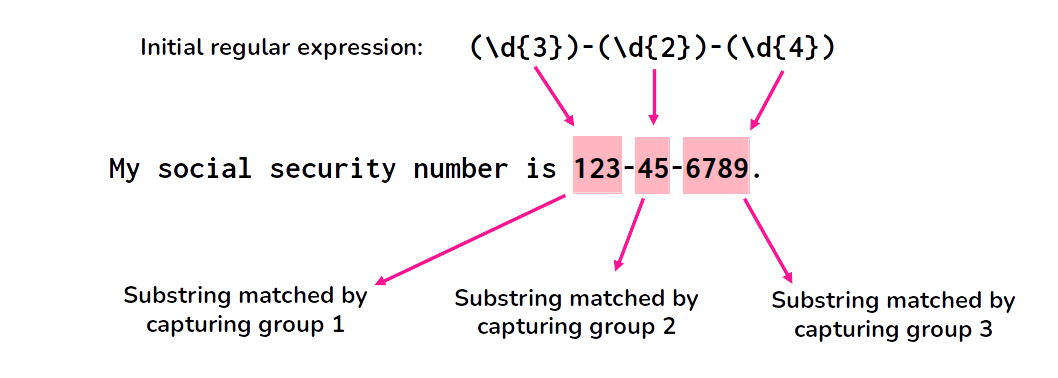
\includegraphics{Chapters/./../Figures/substring-capturing-groups.png}

}

\caption{\label{fig-substring-capturing-groups}Example of capturing
groups}

\end{figure}

In Python, we can access the captured groups using the \texttt{group()}
method of the \texttt{Match} object returned by \texttt{re.search()}. In
this example, \texttt{match.group(1)} returns the captured substring of
the first capturing group (which is \texttt{"123"}),
\texttt{match.group(2)} returns second \texttt{"45"}, and
\texttt{match.group(3)} returns \texttt{"6789"}.

\hypertarget{how-can-we-use-capturing-groups-in-pyspark}{%
\subsubsection{\texorpdfstring{How can we use capturing groups in
\texttt{pyspark}
?}{How can we use capturing groups in pyspark ?}}\label{how-can-we-use-capturing-groups-in-pyspark}}

Ok, now that we understood what capturing groups is, how can we use them
in \texttt{pypspark}? First, remember, capturing groups will be
available to you, only if you enclose a part of your regular expression
in a pair of parentheses. So the first part is to make sure that the
capturing groups are present in your regular expressions.

After that, you can access the substring matched by the capturing group,
by using the reference index that identifies this capturing group you
want to use. In pure Python, we used the \texttt{group()} method with
the group index (like 1, 2, etc.) to access these values.

But in \texttt{pyspark}, we access these groups by using a special
pattern formed by the group index preceded by a dollar sign
(\texttt{\$}). That is, the text \texttt{\$1} references the first
capturing group, \texttt{\$2} references the second capturing group,
etc.

As a first example, lets go back to the regular expression we used at
Section~\ref{sec-regexp-replace}:
\texttt{\textbackslash{}\textbackslash{}{[}(INFO\textbar{}ERROR\textbar{}WARN)\textbackslash{}\textbackslash{}{]}:}.
This regular expression contains one capturing group, which captures the
type label of the log message:
\texttt{(INFO\textbar{}ERROR\textbar{}WARN)}.

If we use the special pattern \texttt{\$1} to reference this capturing
group inside of \texttt{regexp\_replace()}, what is going to happen is:
\texttt{regexp\_replace()} will replace all occurrences of the input
regular expression found on the input string, by the substring matched
by the first capturing group. See in the example below:

\begin{Shaded}
\begin{Highlighting}[]
\NormalTok{logs}\OperatorTok{\textbackslash{}}
\NormalTok{    .withColumn(}
        \StringTok{\textquotesingle{}using\_groups\textquotesingle{}}\NormalTok{,}
\NormalTok{        regexp\_replace(}\StringTok{\textquotesingle{}message\textquotesingle{}}\NormalTok{, type\_regex, }\StringTok{\textquotesingle{}Type Label {-}\textgreater{} $1 | \textquotesingle{}}\NormalTok{)}
\NormalTok{    )}\OperatorTok{\textbackslash{}}
\NormalTok{    .select(}\StringTok{\textquotesingle{}message\textquotesingle{}}\NormalTok{, }\StringTok{\textquotesingle{}using\_groups\textquotesingle{}}\NormalTok{)}\OperatorTok{\textbackslash{}}
\NormalTok{    .show(truncate }\OperatorTok{=} \DecValTok{30}\NormalTok{)}
\end{Highlighting}
\end{Shaded}

\begin{verbatim}
+------------------------------+------------------------------+
|                       message|                  using_groups|
+------------------------------+------------------------------+
|[INFO]: 2022-09-05 03:35:01...|Type Label -> INFO | 2022-0...|
|[WARN]: 2022-09-05 03:35:58...|Type Label -> WARN | 2022-0...|
|[INFO]: 2022-09-05 03:40:59...|Type Label -> INFO | 2022-0...|
|[INFO]: 2022-09-05 03:42:24...|Type Label -> INFO | 2022-0...|
|[INFO]: 2022-09-05 03:42:37...|Type Label -> INFO | 2022-0...|
|[WARN]: 2022-09-05 03:52:02...|Type Label -> WARN | 2022-0...|
|[INFO]: 2022-09-05 04:00:33...|Type Label -> INFO | 2022-0...|
|[INFO]: 2022-09-05 04:01:15...|Type Label -> INFO | 2022-0...|
|[INFO]: 2022-09-05 04:01:35...|Type Label -> INFO | 2022-0...|
|[INFO]: 2022-09-05 04:02:09...|Type Label -> INFO | 2022-0...|
|[INFO]: 2022-09-05 04:02:09...|Type Label -> INFO | 2022-0...|
|[INFO]: 2022-09-05 04:02:09...|Type Label -> INFO | 2022-0...|
|[ERROR]: 2022-09-05 04:02:1...|Type Label -> ERROR | 2022-...|
|[ERROR]: 2022-09-05 04:02:3...|Type Label -> ERROR | 2022-...|
|[ERROR]: 2022-09-05 04:02:3...|Type Label -> ERROR | 2022-...|
|[ERROR]: 2022-09-05 04:02:3...|Type Label -> ERROR | 2022-...|
+------------------------------+------------------------------+
\end{verbatim}

In essence, you can reuse the substrings matched by the capturing
groups, by using the special patterns \texttt{\$1}, \texttt{\$2},
\texttt{\$3}, etc. This means that you can reuse the substrings captured
by multiple groups at the same time inside \texttt{regexp\_replace()}
and \texttt{regexp\_extract()}. For example, if we use the replacement
string \texttt{"\$1,\ \$2,\ \$3"} inside \texttt{regexp\_replace()}, we
would get the substrings matched by the first, second and third
capturing groups, separated by commas.

However, is also good to emphasize a small limitation that this system
has. When you need to reuse the substrings captured by multiple groups
together, is important that you make sure to add some amount of space
(or some delimiter character) between each group reference, like
\texttt{"\$1\ \$2\ \$3"}.

Because if you write these group references one close to each other
(like in \texttt{"\$1\$2\$3"}), it is not going to work. In other words,
Spark will not understand that you are trying to access a capturing
group. It will interpret the text \texttt{"\$1\$2\$3"} as the literal
value \texttt{"\$1\$2\$3"}, and not as a special pattern that references
multiple capturing groups in the regular expression.

\hypertarget{sec-regexp-extract}{%
\subsection{\texorpdfstring{Extracting substrings with
\texttt{regexp\_extract()}}{Extracting substrings with regexp\_extract()}}\label{sec-regexp-extract}}

Another very useful regular expression activity is to extract a
substring from a given string that match a specified regular expression
pattern. The \texttt{regexp\_extract()} function is the main method used
to do this process.

This function takes three arguments, which are:

\begin{itemize}
\tightlist
\item
  The input column name or expression that contains the string to be
  searched;
\item
  The regular expression pattern to search for within the input string;
\item
  The index of the capturing group within the regular expression pattern
  that corresponds to the substring to extract;
\end{itemize}

You may (or may not) use capturing groups inside of
\texttt{regexp\_replace()}. However, on the other hand, the
\texttt{regexp\_extract()} function \textbf{is based on} the capturing
groups functionality. As a consequence, when you use
\texttt{regexp\_extract()}, you must give a regular expression that
\textbf{contains some capturing group}. Because otherwise, the
\texttt{regexp\_extract()} function becomes useless.

In other words, the \texttt{regexp\_extract()} function extracts
substrings that are matched by the capturing groups present in your
input regular expression. If you want, for example, to use
\texttt{regexp\_extract()} to extract the substring matched by a entire
regular expression, then, you just need to surround this entire regular
expression by a pair of parentheses. This way you transform this entire
regular expression in a capturing group, and, therefore, you can extract
the substring matched by this group.

As an example, lets go back again to the regular expression we used in
the \texttt{logs} DataFrame:
\texttt{\textbackslash{}\textbackslash{}{[}(INFO\textbar{}ERROR\textbar{}WARN)\textbackslash{}\textbackslash{}{]}:}.
We can extract the type of log message label, by using the index 1 to
reference the first (and only) capturing group in this regular
expression.

\begin{Shaded}
\begin{Highlighting}[]
\ImportTok{from}\NormalTok{ pyspark.sql.functions }\ImportTok{import}\NormalTok{ regexp\_extract}

\NormalTok{logs}\OperatorTok{\textbackslash{}}
\NormalTok{    .withColumn(}
        \StringTok{\textquotesingle{}message\_type\textquotesingle{}}\NormalTok{,}
\NormalTok{        regexp\_extract(}\StringTok{\textquotesingle{}message\textquotesingle{}}\NormalTok{, type\_regex, }\DecValTok{1}\NormalTok{)}
\NormalTok{    )}\OperatorTok{\textbackslash{}}
\NormalTok{    .select(}\StringTok{\textquotesingle{}message\textquotesingle{}}\NormalTok{, }\StringTok{\textquotesingle{}message\_type\textquotesingle{}}\NormalTok{)}\OperatorTok{\textbackslash{}}
\NormalTok{    .show(truncate }\OperatorTok{=} \DecValTok{30}\NormalTok{)}
\end{Highlighting}
\end{Shaded}

\begin{verbatim}
+------------------------------+------------+
|                       message|message_type|
+------------------------------+------------+
|[INFO]: 2022-09-05 03:35:01...|        INFO|
|[WARN]: 2022-09-05 03:35:58...|        WARN|
|[INFO]: 2022-09-05 03:40:59...|        INFO|
|[INFO]: 2022-09-05 03:42:24...|        INFO|
|[INFO]: 2022-09-05 03:42:37...|        INFO|
|[WARN]: 2022-09-05 03:52:02...|        WARN|
|[INFO]: 2022-09-05 04:00:33...|        INFO|
|[INFO]: 2022-09-05 04:01:15...|        INFO|
|[INFO]: 2022-09-05 04:01:35...|        INFO|
|[INFO]: 2022-09-05 04:02:09...|        INFO|
|[INFO]: 2022-09-05 04:02:09...|        INFO|
|[INFO]: 2022-09-05 04:02:09...|        INFO|
|[ERROR]: 2022-09-05 04:02:1...|       ERROR|
|[ERROR]: 2022-09-05 04:02:3...|       ERROR|
|[ERROR]: 2022-09-05 04:02:3...|       ERROR|
|[ERROR]: 2022-09-05 04:02:3...|       ERROR|
+------------------------------+------------+
\end{verbatim}

As another example, lets suppose we wanted to extract not only the type
of the log message, but also, the timestamp and the content of the
message, and store these different elements in separate columns.

To do that, we could build a more complete regular expression. An
expression capable of matching the entire log message, and, at the same
time, capture each of these different elements inside a different
capturing group. The code below is an example that produces such regular
expression, and applies it over the \texttt{logs} DataFrame.

\begin{Shaded}
\begin{Highlighting}[]
\NormalTok{type\_regex }\OperatorTok{=} \VerbatimStringTok{r\textquotesingle{}\textbackslash{}[(INFO|ERROR|WARN)\textbackslash{}]: \textquotesingle{}}

\NormalTok{date\_regex }\OperatorTok{=} \VerbatimStringTok{r\textquotesingle{}\textbackslash{}d}\SpecialCharTok{\{4\}}\VerbatimStringTok{{-}\textbackslash{}d}\SpecialCharTok{\{2\}}\VerbatimStringTok{{-}\textbackslash{}d}\SpecialCharTok{\{2\}}\VerbatimStringTok{\textquotesingle{}}
\NormalTok{time\_regex }\OperatorTok{=} \VerbatimStringTok{r\textquotesingle{} \textbackslash{}d}\SpecialCharTok{\{2\}}\VerbatimStringTok{:\textbackslash{}d}\SpecialCharTok{\{2\}}\VerbatimStringTok{:\textbackslash{}d}\SpecialCharTok{\{2\}}\VerbatimStringTok{([.]\textbackslash{}d+)?\textquotesingle{}}
\NormalTok{timestamp\_regex }\OperatorTok{=}\NormalTok{ date\_regex }\OperatorTok{+}\NormalTok{ time\_regex}
\NormalTok{timestamp\_regex }\OperatorTok{=} \VerbatimStringTok{r\textquotesingle{}(\textquotesingle{}} \OperatorTok{+}\NormalTok{ timestamp\_regex }\OperatorTok{+} \VerbatimStringTok{r\textquotesingle{})\textquotesingle{}}

\NormalTok{regex }\OperatorTok{=}\NormalTok{ type\_regex }\OperatorTok{+}\NormalTok{ timestamp\_regex }\OperatorTok{+} \VerbatimStringTok{r\textquotesingle{}(.+)$\textquotesingle{}}

\NormalTok{logs}\OperatorTok{\textbackslash{}}
\NormalTok{    .withColumn(}
        \StringTok{\textquotesingle{}message\_type\textquotesingle{}}\NormalTok{,}
\NormalTok{        regexp\_extract(}\StringTok{\textquotesingle{}message\textquotesingle{}}\NormalTok{, regex, }\DecValTok{1}\NormalTok{)}
\NormalTok{    )}\OperatorTok{\textbackslash{}}
\NormalTok{    .withColumn(}
        \StringTok{\textquotesingle{}timestamp\textquotesingle{}}\NormalTok{,}
\NormalTok{        regexp\_extract(}\StringTok{\textquotesingle{}message\textquotesingle{}}\NormalTok{, regex, }\DecValTok{2}\NormalTok{)}
\NormalTok{    )}\OperatorTok{\textbackslash{}}
\NormalTok{    .withColumn(}
        \StringTok{\textquotesingle{}message\_content\textquotesingle{}}\NormalTok{,}
\NormalTok{        regexp\_extract(}\StringTok{\textquotesingle{}message\textquotesingle{}}\NormalTok{, regex, }\DecValTok{4}\NormalTok{)}
\NormalTok{    )}\OperatorTok{\textbackslash{}}
\NormalTok{    .select(}\StringTok{\textquotesingle{}message\_type\textquotesingle{}}\NormalTok{, }\StringTok{\textquotesingle{}timestamp\textquotesingle{}}\NormalTok{, }\StringTok{\textquotesingle{}message\_content\textquotesingle{}}\NormalTok{)}\OperatorTok{\textbackslash{}}
\NormalTok{    .show(}\DecValTok{5}\NormalTok{, truncate }\OperatorTok{=} \DecValTok{30}\NormalTok{)}
\end{Highlighting}
\end{Shaded}

\begin{verbatim}
+------------+-----------------------+------------------------------+
|message_type|              timestamp|               message_content|
+------------+-----------------------+------------------------------+
|        INFO| 2022-09-05 03:35:01.43| Looking for workers at Sou...|
|        WARN|2022-09-05 03:35:58.007| Workers are unavailable at...|
|        INFO|2022-09-05 03:40:59.054| Looking for workers at Sou...|
|        INFO|    2022-09-05 03:42:24| 3 Workers were acquired at...|
|        INFO|    2022-09-05 03:42:37| Initializing instances in ...|
+------------+-----------------------+------------------------------+
only showing top 5 rows
\end{verbatim}

\hypertarget{identifying-values-that-match-a-particular-regular-expression-with-rlike}{%
\subsection{\texorpdfstring{Identifying values that match a particular
regular expression with
\texttt{rlike()}}{Identifying values that match a particular regular expression with rlike()}}\label{identifying-values-that-match-a-particular-regular-expression-with-rlike}}

The \texttt{rlike()} column method is useful for checking if a string
value in a column matches a specific regular expression. We briefly
introduced this methd at Section~\ref{sec-filter-regex-pattern}. This
method has only one input, which is the regular expression you want to
apply over the column values.

As an example, lets suppose you wanted to identify timestamp values
inside your strings. You could use a regular expression pattern to find
which text values had these kinds of values inside them.

A possible regular expression candidate for it would be
\texttt{"{[}0-9{]}\{2\}:{[}0-9{]}\{2\}:{[}0-9{]}\{2\}({[}.{]}{[}0-9{]}+)?"}.
This regex matches timestamp values in the format ``hh:mm:ss.sss''. This
pattern consists of the following building blocks, or, elements:

\begin{itemize}
\tightlist
\item
  \texttt{{[}0-9{]}\{2\}}: Matches any two digits from 0 to 9.
\item
  \texttt{:}: Matches a colon character.
\item
  \texttt{({[}.{]}{[}0-9{]}+)?}: Matches an optional decimal point
  followed by one or more digits.
\end{itemize}

If we apply this pattern over all log messages stored in the
\texttt{logs} DataFrame, we would find that all logs messages matches
this particular regular expression. Because all log messages contains a
timestamp value at the start of the message:

\begin{Shaded}
\begin{Highlighting}[]
\ImportTok{from}\NormalTok{ pyspark.sql.functions }\ImportTok{import}\NormalTok{ col}

\NormalTok{pattern }\OperatorTok{=} \StringTok{"[0{-}9]}\SpecialCharTok{\{2\}}\StringTok{:[0{-}9]}\SpecialCharTok{\{2\}}\StringTok{:[0{-}9]}\SpecialCharTok{\{2\}}\StringTok{([.][0{-}9]+)?"}
\NormalTok{logs}\OperatorTok{\textbackslash{}}
\NormalTok{    .withColumn(}
        \StringTok{\textquotesingle{}does\_it\_match?\textquotesingle{}}\NormalTok{,}
\NormalTok{        col(}\StringTok{"message"}\NormalTok{).rlike(pattern)}
\NormalTok{    )}\OperatorTok{\textbackslash{}}
\NormalTok{    .select(}\StringTok{\textquotesingle{}message\textquotesingle{}}\NormalTok{, }\StringTok{\textquotesingle{}does\_it\_match?\textquotesingle{}}\NormalTok{)}\OperatorTok{\textbackslash{}}
\NormalTok{    .show(}\DecValTok{5}\NormalTok{, truncate }\OperatorTok{=}\NormalTok{ n\_truncate)}
\end{Highlighting}
\end{Shaded}

\begin{verbatim}
+--------------------------------------------------+--------------+
|                                           message|does_it_match?|
+--------------------------------------------------+--------------+
|[INFO]: 2022-09-05 03:35:01.43 Looking for work...|          true|
|[WARN]: 2022-09-05 03:35:58.007 Workers are una...|          true|
|[INFO]: 2022-09-05 03:40:59.054 Looking for wor...|          true|
|[INFO]: 2022-09-05 03:42:24 3 Workers were acqu...|          true|
|[INFO]: 2022-09-05 03:42:37 Initializing instan...|          true|
+--------------------------------------------------+--------------+
only showing top 5 rows
\end{verbatim}

\bookmarksetup{startatroot}

\hypertarget{references}{%
\chapter*{References}\label{references}}
\addcontentsline{toc}{chapter}{References}

\markboth{References}{References}

\hypertarget{refs}{}
\begin{CSLReferences}{1}{0}
\leavevmode\vadjust pre{\hypertarget{ref-sparkdoc}{}}%
\emph{Apache Spark Official Documentation}. 2022. Documentation for
Apache Spark 3.2.1. \url{https://spark.apache.org/docs/latest/}.

\leavevmode\vadjust pre{\hypertarget{ref-chambers2018}{}}%
Chambers, Bill, and Matei Zaharia. 2018. \emph{Spark: The Definitive
Guide: Big Data Processing Made Simple}. Sebastopol, CA: O'Reilly Media.

\leavevmode\vadjust pre{\hypertarget{ref-damji2020}{}}%
Damji, Jules, Brooke Wenig, Tathagata Das, and Denny Lee. 2020.
\emph{Learning Spark: Lightning-Fast Data Analytics}. Sebastopol, CA:
O'Reilly Media.

\leavevmode\vadjust pre{\hypertarget{ref-regexinfo}{}}%
Goyvaerts, Jan. 2023. {``Regular-Expressions.info.''}
\url{https://www.regular-expressions.info/}.

\leavevmode\vadjust pre{\hypertarget{ref-karau2015}{}}%
Karau, Holden, Andy Konwinski, Patrick Wendell, and Matei Zaharia. 2015.
\emph{Learning Spark: Lightning-Fast Data Analytics}. Sebastopol, CA:
O'Reilly Media.

\end{CSLReferences}

\appendix
\addcontentsline{toc}{part}{Appendices}

\hypertarget{sec-open-terminal}{%
\chapter{Opening the terminal of your OS}\label{sec-open-terminal}}

Every operating system (OS) comes with a terminal (or a command prompt).
A terminal is usually just a black screen where you can send commands to
be executed by your OS. As an example,
Figure~\ref{fig-terminal-simple-shot} shows a print screen of the
terminal in Ubuntu Linux. The terminal on Windows is very similar to
this.

\begin{figure}

{\centering 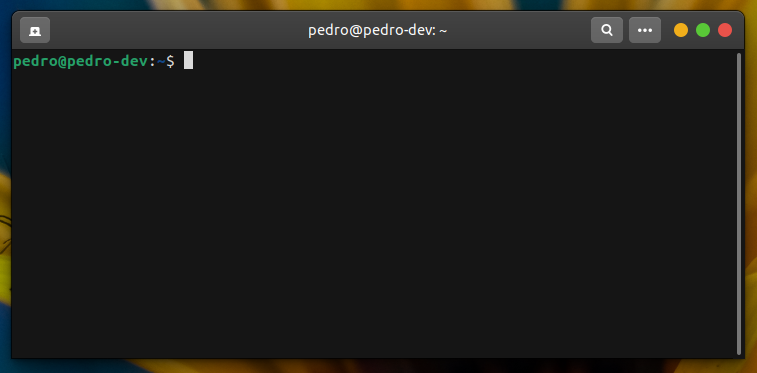
\includegraphics{Chapters/./../Figures/terminal-simple-shot.png}

}

\caption{\label{fig-terminal-simple-shot}A terminal on Ubuntu}

\end{figure}

Terminals are incredibely flexible tools, and you will find this tool
very useful for a number of things. However, since they are just a black
and empty screen, they give you no clue of what you should do, or what
commands are available to you.

That is ok, for now, you should not worry about that. I will expose many
terminal commands in this book, and these commands should be used inside
these terminals that comes with your OS. The next sub-sections will show
you how to open a terminal in each one of the OS's where Spark is
available. Lets begin with Windows.

\hypertarget{opening-a-terminal-on-windows}{%
\subsection{Opening a terminal on
Windows}\label{opening-a-terminal-on-windows}}

There are some different approaches to do this, but, the one that I find
the most useful, is to open a terminal from inside a folder, using the
default File Explorer program of Windows.

This is very useful, because we normally use terminal commands to affect
a set of files that are stored inside a specific folder in our computer.

As a result, when we open a terminal from inside a folder, using the
File Explorer, the terminal opened is already rooted inside the folder
where our files are stored. In other words, we already have easy access
to the files that we want to affect/use in our command, and we do not
have the work to change or adjust directories in this terminal.

For example, lets suppose that we want to use a terminal command to use
a file called \texttt{hello.py}, and, that this \texttt{hello.py} file
is stored inside a folder called \texttt{HelloPython}. You can see in
Figure~\ref{fig-windows-hello-folder}, that this folder is in path
\texttt{C:\textbackslash{}Users\textbackslash{}pedro\textbackslash{}Documents\textbackslash{}HelloPython}.
So, the first step, is to use the File Explorer of Windows, to open this
folder, like in Figure~\ref{fig-windows-hello-folder}.

\begin{figure}

{\centering 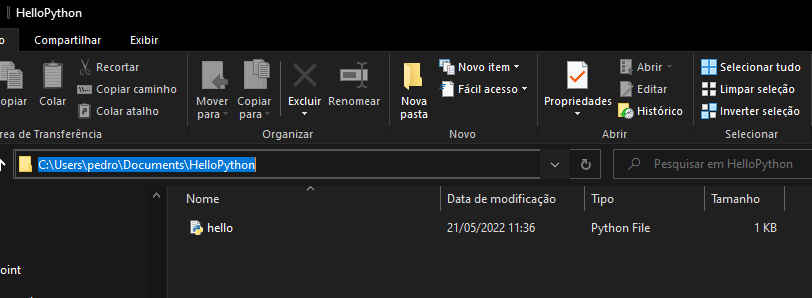
\includegraphics{Chapters/../Figures/windows-hello-folder.png}

}

\caption{\label{fig-windows-hello-folder}Opening the
\texttt{HelloPython} folder in Windows}

\end{figure}

After you opened this folder, substitute the path to the folder in the
search box with the word ``cmd'', like in
Figure~\ref{fig-windows-hello-folder2}, and them, press Enter in the
keyboard.

\begin{figure}

{\centering 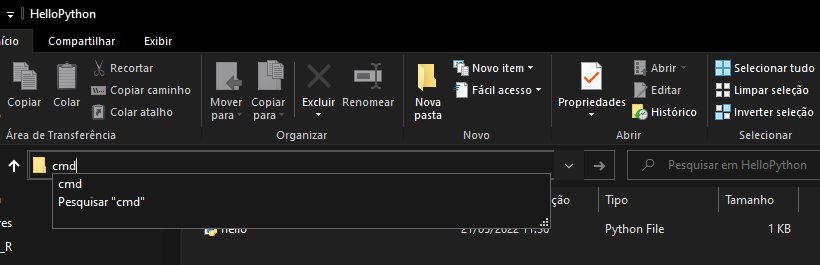
\includegraphics{Chapters/../Figures/windows-hello-folder2.png}

}

\caption{\label{fig-windows-hello-folder2}Opening a terminal inside a
Windows folder - Part 1}

\end{figure}

As a result, a new terminal will open. See in
Figure~\ref{fig-windows-terminal}, that this new terminal is already
looking to (or is already rooted on) this \texttt{HelloPython} folder.
This way, we can easily access the files stored inside this folder, like
the \texttt{hello.py} file.

\begin{figure}

{\centering 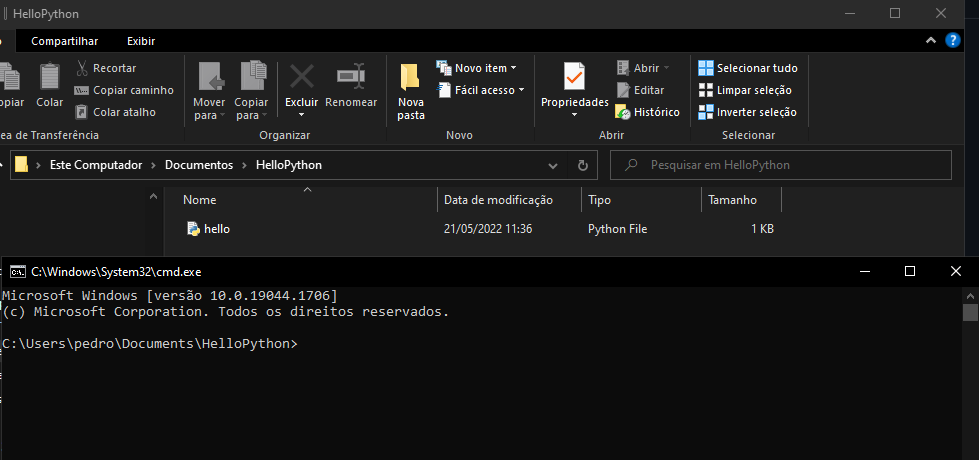
\includegraphics{Chapters/../Figures/windows-terminal.png}

}

\caption{\label{fig-windows-terminal}Opening a terminal inside a Windows
folder - Part 2}

\end{figure}

\hypertarget{opening-a-terminal-on-linux}{%
\subsection{Opening a terminal on
Linux}\label{opening-a-terminal-on-linux}}

Is fairly easy to open a terminal on a Linux distribution. Again, is
very useful when you open the terminal from inside the folder you are
interested in. Because you will have an easier access to all the files
that are stored inside this folder.

To do this in Linux, you use the built-in File Explorer to open the
folder where you want to root your terminal. At the moment, I am using
an Ubuntu distribution. I just opened the same \texttt{HelloPython}
folder, with the same \texttt{hello.py} file, in the File Explorer of
Linux. As shown in Figure~\ref{fig-ubuntu-folder}:

\begin{figure}

{\centering 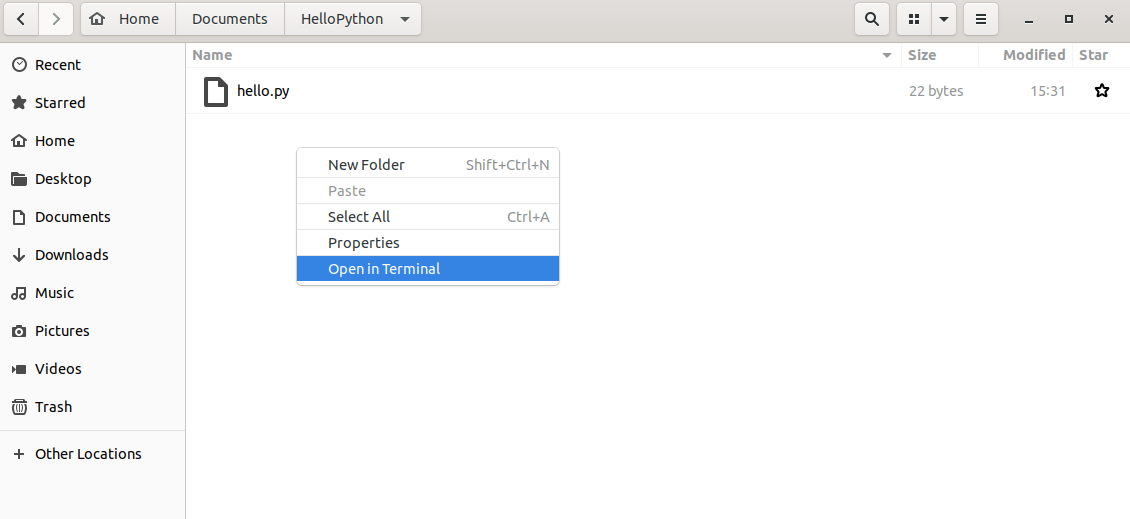
\includegraphics{Chapters/../Figures/ubuntu-folder.png}

}

\caption{\label{fig-ubuntu-folder}Opening the \texttt{HelloPython}
folder in Linux}

\end{figure}

After you opened the folder, just click with the right button of your
mouse, and select the ``Open in Terminal'' option, and a new terminal
should appear on your screen. See in
Figure~\ref{fig-ubuntu-folder-terminal}, that the new terminal is
already looking to the \texttt{HelloPython} folder, as we expected.

\begin{figure}

{\centering 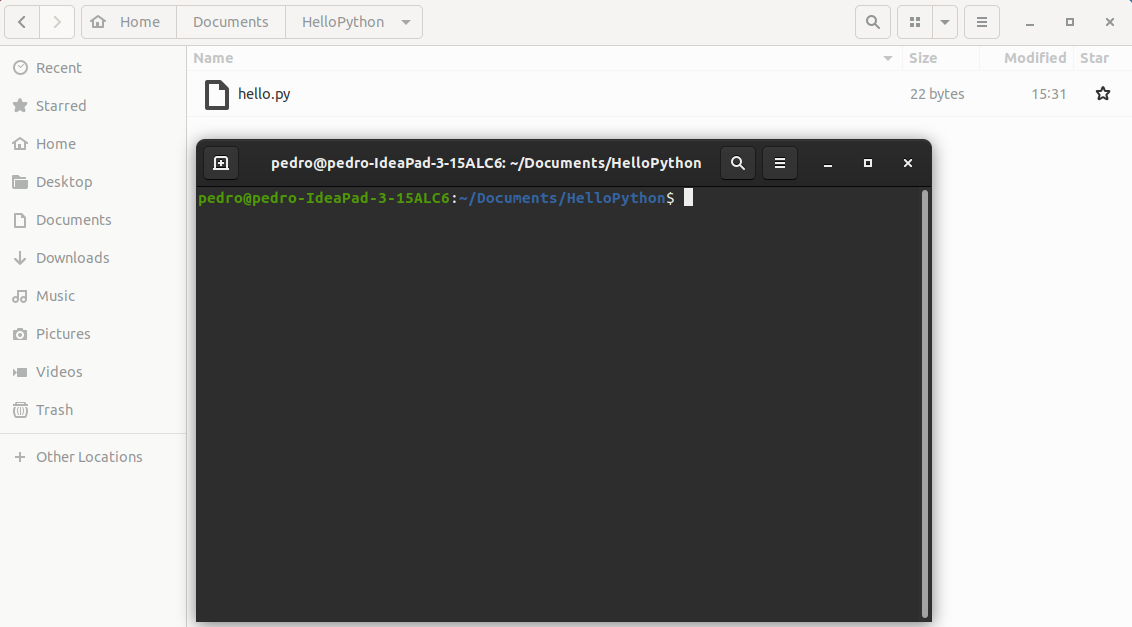
\includegraphics{Chapters/../Figures/ubuntu-folder-terminal.png}

}

\caption{\label{fig-ubuntu-folder-terminal}Opening the terminal in
Linux}

\end{figure}

\hypertarget{opening-a-terminal-in-macos}{%
\subsection{Opening a terminal in
MacOs}\label{opening-a-terminal-in-macos}}

Unfortunately, I do not have a Mac machine in my possession, so I cannot
easily show you how to open a terminal in MacOs. But there a lot of
articles available in the internet discussing how to open a terminal in
MacOs. For example, there is a article from the support of
Apple\footnote{\url{https://support.apple.com/en-ie/guide/terminal/apd5265185d-f365-44cb-8b09-71a064a42125/mac}},
or this other article from iDownloadBlog\footnote{\url{https://www.idownloadblog.com/2019/04/19/ways-open-terminal-mac/}}.

\hypertarget{sec-install-spark}{%
\chapter{\texorpdfstring{How to install Spark and
\texttt{pyspark}}{How to install Spark and pyspark}}\label{sec-install-spark}}

In order to build and run any Spark application through
\texttt{pyspark}, you have to install Apache Spark in your computer.
Apache Spark is available to all three major operating systems in the
market today (macOS, Windows and Linux).

The process of installation is kind of similar in all three OS's. But
some steps work differently in each OS. Currently, I (the author of this
book) do not have access to a macOS machine, and because of that, I will
not describe the installation process of Spark on this platform here. If
you have access to a macOS machine, and are willing to describe this
installation process, I would be happy to review a PR with such content.

\hypertarget{what-are-the-steps}{%
\section{What are the steps?}\label{what-are-the-steps}}

In short, the next steps for installing Spark are:

\begin{enumerate}
\def\labelenumi{\arabic{enumi}.}
\tightlist
\item
  Install Java;
\item
  Install Python;
\item
  Install \texttt{pyspark};
\item
  Download and extract Apache Spark;
\item
  Set a few environment variables;
\end{enumerate}

The next sections describes these steps for each operating system.

\hypertarget{on-windows}{%
\section{On Windows}\label{on-windows}}

\hypertarget{install-java-sdk}{%
\subsection{Install Java SDK}\label{install-java-sdk}}

Apache Spark is written in Scala, which is a fairly modern programming
language that have powerful interoperability with the Java programming
language. Because of this characteristic, some of the functionalities of
Spark require you to have Java SDK (\emph{Software Development Kit})
installed in your machine.

In other words, you must have Java SDK installed to use Spark. If you do
not have Java SDK, Spark will likely fail when you try to start it.
However, since Java is a very popular tecnology across the world, is
possible that you already have it installed in your machine. To check if
Java is already installed, you can run the following command in your OS
terminal:

\begin{Shaded}
\begin{Highlighting}[]
\NormalTok{\#| eval: false}
\NormalTok{Terminal$ java {-}version}
\end{Highlighting}
\end{Shaded}

If the above command outputs something similar to the text exposed
below, than, you already have Java installed in your machine, and you
can proceed to the next step.

\begin{verbatim}
java version "19.0.1" 2022-10-18
Java(TM) SE Runtime Environment (build 19.0.1+10-21)
Java HotSpot(TM) 64-Bit Server VM (build 19.0.1+10-21, mixed mode, sharing)
\end{verbatim}

But, if something different comes up in your terminal, than, is likely
that you do not have Java installed. To fix this,
\href{https://www.oracle.com/java/technologies/downloads/}{download Java
from the official website}\footnote{\url{https://www.oracle.com/java/technologies/downloads/}},
and install it.

\hypertarget{install-python}{%
\subsection{Install Python}\label{install-python}}

You can easily install Python on Windows, by downloading the installer
available at the \href{https://www.python.org/downloads/}{official
website of the language}\footnote{\url{https://www.python.org/downloads/}},
and executing it.

\hypertarget{install-pyspark}{%
\subsection{\texorpdfstring{Install
\texttt{pyspark}}{Install pyspark}}\label{install-pyspark}}

Installing the \texttt{pyspark} python package is pretty
straightforward. Just open a terminal (if you need help to open the
terminal check Appendix~\ref{sec-open-terminal}), and use the
\texttt{pip} command to do it:

\begin{Shaded}
\begin{Highlighting}[]
\NormalTok{\#| eval: false}
\NormalTok{Terminal$ pip install pyspark}
\end{Highlighting}
\end{Shaded}

If you try to run the above command (inside a terminal of any OS), and a
message like \texttt{pip:\ command\ not\ found} appears, this means that
you do not have the \texttt{pip} tool installed on your machine. Hence,
if you face this kind of message, you need to install \texttt{pip}
before you even install \texttt{pyspark}.

The \texttt{pip} tool is automatically installed with Python on Windows.
So, if you face this message (\texttt{pip:\ command\ not\ found}), then,
is very likely that you do not have Python correctly installed on your
machine. Or maybe, Python is not installed at all in any shape or size
in your system. So, you should comeback to previous section, and re
install it.

\hypertarget{download-and-extract-the-files-of-apache-spark}{%
\subsection{Download and extract the files of Apache
Spark}\label{download-and-extract-the-files-of-apache-spark}}

First, you need to download Apache Spark from the
\href{https://spark.apache.org/downloads}{official website of the
project}\footnote{\url{https://spark.apache.org/downloads}}. Currently,
the Apache Spark does not offers installers or package programs to
install the software for you.

We usually install external software on Windows by using installers
(i.e.~executable files - \texttt{.exe}) that perform all the necessary
steps to install the software in your machine. However, currently, the
Apache Spark project does not offers such installers. This means that
you have to install it yourself.

When you download Apache Spark from the official website, you will get
all files of the program compacted inside a TAR file (\texttt{.tgz}),
which is similar to a ZIP file (\texttt{.zip}). After you downloaded
Spark to your machine, you need to extract all files from the TAR file
(\texttt{.tgz}) to a specific location of your computer. It can be
anywhere, just choose a place. As an example, I will extract the files
to a folder called \texttt{Spark} directly at my hard disk \texttt{C:/}.

To extract these files, you can use very popular UI tools like
\href{https://7-zip.org/}{7zip}\footnote{\url{https://7-zip.org/}} or
\href{https://www.win-rar.com/}{WinRAR}\footnote{\url{https://www.win-rar.com/}}.
However, if you use a modern version of Windows, there is a \texttt{tar}
command line tool available at the terminal that you can use to do this
process in a programatic fashion. As an example, I can extract and move
all files of Spark with these commands:

\begin{Shaded}
\begin{Highlighting}[]
\NormalTok{\#| eval: false}
\NormalTok{Terminal$ tar {-}x {-}f spark{-}3.3.1{-}bin{-}hadoop3.tgz}
\NormalTok{Terminal$ mv spark{-}3.3.1{-}bin{-}hadoop3 C:/Spark/spark{-}3.3.1{-}bin{-}hadoop3}
\end{Highlighting}
\end{Shaded}

\hypertarget{set-environment-variables}{%
\subsection{Set environment variables}\label{set-environment-variables}}

Apache Spark will always look for two specific environment variables in
your system: \texttt{SPARK\_HOME} and \texttt{JAVA\_HOME}. This means
that you must have these two environment variables defined and correctly
configured in your machine. To configure an environment variable on
Windows, I recommend you to use the menu that you can find by searching
for ``environment variables'' in the Windows search box. At
Figure~\ref{fig-windows-envs} you can see the path to this menu on
Windows:

\begin{figure}

{\centering 

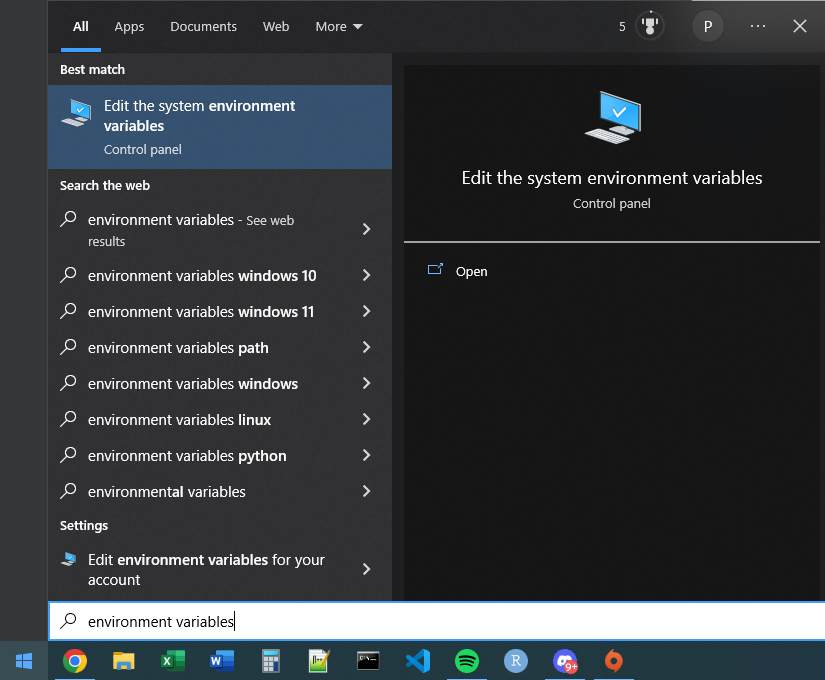
\includegraphics{Chapters/../Figures/windows-environment-variables1.png}\{\#fig-windows-env1,
fig-env=``subfigure''\}

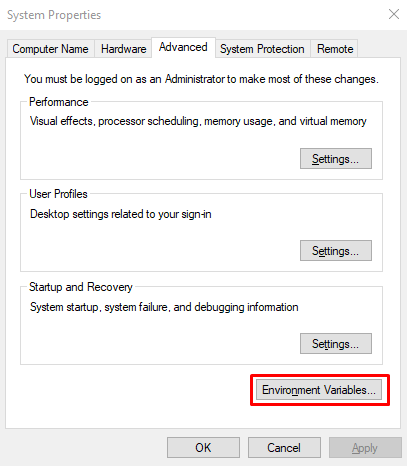
\includegraphics{Chapters/../Figures/windows-environment-variables2.png}\{\#fig-windows-env2,
fig-env=``subfigure''\}

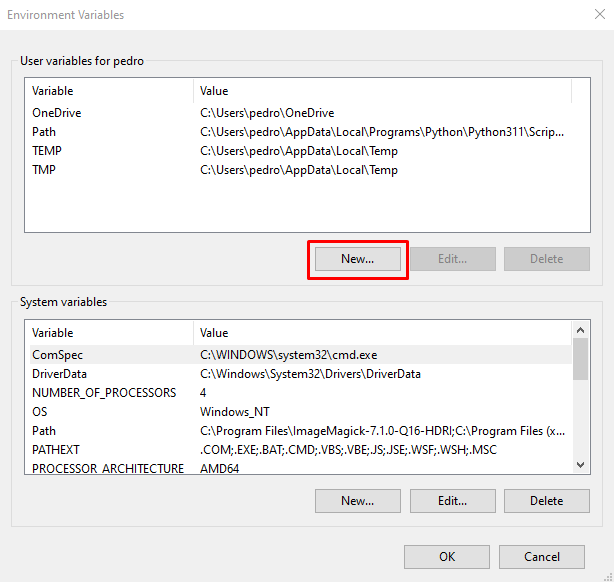
\includegraphics{Chapters/../Figures/windows-environment-variables3.png}\{\#fig-windows-env3,
fig-env=``subfigure''\}

}

\caption{\label{fig-windows-envs}Path to Windows Environment Variables
Menu}

\end{figure}

During the process of scheduling and running your Spark application,
Spark will execute a set of scripts located at the home directory of
Spark itself. Spark does this by looking for a environment variable
called \texttt{SPARK\_HOME} in your system. If you do not have this
variable configured, Spark will not be able to locate its home
directory, and as a consequence, it throws an runtime error.

In other words, you need to set a variable with name
\texttt{SPARK\_HOME} in your system. Its value should be the path to the
home (or ``root'') directory where you installed (or unzipped) the Spark
files. In my case I unzipped the files into a folder called
\texttt{C:/Spark/spark-3.3.1-bin-hadoop3}, and that is the folder that I
going to use in \texttt{SPARK\_HOME}, as you can see at
Figure~\ref{fig-spark-home-env}:

\begin{figure}

{\centering 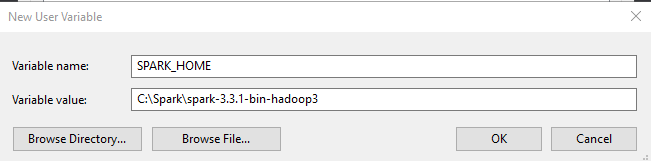
\includegraphics{Chapters/../Figures/windows-environment-variables4.png}

}

\caption{\label{fig-spark-home-env}Setting the \texttt{SPARK\_HOME}
environment variable}

\end{figure}

Now, a lot Spark functionality is closely related to Java SDK, and to
find it, Spark will look for a environment variable called
\texttt{JAVA\_HOME}. On my machine, I have Java SDK installed at the
folder
\texttt{C:\textbackslash{}Program\ Files\textbackslash{}Java\textbackslash{}jdk-19}.
This might be not your case, and you may find the ``jdk'' folder for
Java at a different location of your computer. Just find where it is,
and use this path while setting this \texttt{JAVA\_HOME} variable, like
I did at Figure~\ref{fig-java-home-env}:

\begin{figure}

{\centering 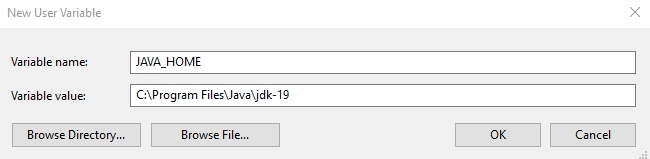
\includegraphics{Chapters/../Figures/windows-environment-variables5.png}

}

\caption{\label{fig-java-home-env}Setting the \texttt{JAVA\_HOME}
environment variable}

\end{figure}

With these two environment variables setted, you should be able to start
and use Spark already. Just open a brand new terminal, and type the
\texttt{spark} command. An interactive Spark Session will initiate after
this command, and give you a command prompt where you can start coding
the Spark application you want to execute.

\hypertarget{on-linux}{%
\section{On Linux}\label{on-linux}}

\hypertarget{install-pyspark-1}{%
\subsection{\texorpdfstring{Install
\texttt{pyspark}}{Install pyspark}}\label{install-pyspark-1}}

In Linux systems, installing \texttt{pip} is very easy, because you can
use the built-in package manager to do this for you. In Debian like
distros (e.g.~Ubuntu), you use the \texttt{apt} tool, and, in Arch-Linux
like distros (e.g.~Arch Linux, Manjaro) you would use the
\texttt{pacman} tool. Both possibilities are exposed below:

\texttt{\{terminal,\ eval\ =\ FALSE\}\ \#\ If\ you\ are\ in\ a\ Debian\ like\ distro\ of\ Linux\ \#\ and\ need\ to\ install\ \textasciigrave{}pip\textasciigrave{},\ use\ this\ command:\ Terminal\$\ sudo\ apt\ install\ python3-pip\ \#\ If\ you\ are\ in\ a\ Arch-Linux\ like\ distro\ of\ Linux\ \#\ and\ need\ to\ install\ \textasciigrave{}pip\textasciigrave{},\ use\ this\ command:\ Terminal\$\ pacman\ -S\ python-pip}



\end{document}
